\documentclass[twoside]{book}

% Packages required by doxygen
\usepackage{fixltx2e}
\usepackage{calc}
\usepackage{doxygen}
\usepackage{graphicx}
\usepackage[utf8]{inputenc}
\usepackage{makeidx}
\usepackage{multicol}
\usepackage{multirow}
\PassOptionsToPackage{warn}{textcomp}
\usepackage{textcomp}
\usepackage[nointegrals]{wasysym}
\usepackage[table]{xcolor}

% Font selection
\usepackage[T1]{fontenc}
\usepackage{mathptmx}
\usepackage[scaled=.90]{helvet}
\usepackage{courier}
\usepackage{amssymb}
\usepackage{sectsty}
\renewcommand{\familydefault}{\sfdefault}
\allsectionsfont{%
  \fontseries{bc}\selectfont%
  \color{darkgray}%
}
\renewcommand{\DoxyLabelFont}{%
  \fontseries{bc}\selectfont%
  \color{darkgray}%
}
\newcommand{\+}{\discretionary{\mbox{\scriptsize$\hookleftarrow$}}{}{}}

% Page & text layout
\usepackage{geometry}
\geometry{%
  a4paper,%
  top=2.5cm,%
  bottom=2.5cm,%
  left=2.5cm,%
  right=2.5cm%
}
\tolerance=750
\hfuzz=15pt
\hbadness=750
\setlength{\emergencystretch}{15pt}
\setlength{\parindent}{0cm}
\setlength{\parskip}{0.2cm}
\makeatletter
\renewcommand{\paragraph}{%
  \@startsection{paragraph}{4}{0ex}{-1.0ex}{1.0ex}{%
    \normalfont\normalsize\bfseries\SS@parafont%
  }%
}
\renewcommand{\subparagraph}{%
  \@startsection{subparagraph}{5}{0ex}{-1.0ex}{1.0ex}{%
    \normalfont\normalsize\bfseries\SS@subparafont%
  }%
}
\makeatother

% Headers & footers
\usepackage{fancyhdr}
\pagestyle{fancyplain}
\fancyhead[LE]{\fancyplain{}{\bfseries\thepage}}
\fancyhead[CE]{\fancyplain{}{}}
\fancyhead[RE]{\fancyplain{}{\bfseries\leftmark}}
\fancyhead[LO]{\fancyplain{}{\bfseries\rightmark}}
\fancyhead[CO]{\fancyplain{}{}}
\fancyhead[RO]{\fancyplain{}{\bfseries\thepage}}
\fancyfoot[LE]{\fancyplain{}{}}
\fancyfoot[CE]{\fancyplain{}{}}
\fancyfoot[RE]{\fancyplain{}{\bfseries\scriptsize Generated on Fri Dec 2 2016 08\+:54\+:32 for cpp-\/atmi by Doxygen }}
\fancyfoot[LO]{\fancyplain{}{\bfseries\scriptsize Generated on Fri Dec 2 2016 08\+:54\+:32 for cpp-\/atmi by Doxygen }}
\fancyfoot[CO]{\fancyplain{}{}}
\fancyfoot[RO]{\fancyplain{}{}}
\renewcommand{\footrulewidth}{0.4pt}
\renewcommand{\chaptermark}[1]{%
  \markboth{#1}{}%
}
\renewcommand{\sectionmark}[1]{%
  \markright{\thesection\ #1}%
}

% Indices & bibliography
\usepackage{natbib}
\usepackage[titles]{tocloft}
\setcounter{tocdepth}{3}
\setcounter{secnumdepth}{5}
\makeindex

% Hyperlinks (required, but should be loaded last)
\usepackage{ifpdf}
\ifpdf
  \usepackage[pdftex,pagebackref=true]{hyperref}
\else
  \usepackage[ps2pdf,pagebackref=true]{hyperref}
\fi
\hypersetup{%
  colorlinks=true,%
  linkcolor=blue,%
  citecolor=blue,%
  unicode%
}

% Custom commands
\newcommand{\clearemptydoublepage}{%
  \newpage{\pagestyle{empty}\cleardoublepage}%
}


%===== C O N T E N T S =====

\begin{document}

% Titlepage & ToC
\hypersetup{pageanchor=false,
             bookmarks=true,
             bookmarksnumbered=true,
             pdfencoding=unicode
            }
\pagenumbering{roman}
\begin{titlepage}
\vspace*{7cm}
\begin{center}%
{\Large cpp-\/atmi \\[1ex]\large (S\+N\+A\+P\+S\+H\+O\+T) }\\
\vspace*{1cm}
{\large Generated by Doxygen 1.8.8}\\
\vspace*{0.5cm}
{\small Fri Dec 2 2016 08:54:32}\\
\end{center}
\end{titlepage}
\clearemptydoublepage
\tableofcontents
\clearemptydoublepage
\pagenumbering{arabic}
\hypersetup{pageanchor=true}

%--- Begin generated contents ---
\chapter{Main Page}
\label{index}\hypertarget{index}{}\subsubsection*{What it does}

A\+T\+M\+I, for Application-\/to-\/\+Transaction Monitor Interface, is the main A\+P\+I for the Tuxedo system. It includes transaction management functions (routines, verbs); request/response, conversational, queuing, and publish-\/and-\/subscribe message-\/handling functions; service interface functions; and buffer management functions for distributed application communication.

A\+T\+M\+I++ is a C++ wrapping of this A\+P\+I, adding strong typing of F\+M\+L buffers and adding the use of exceptions to detect and handle error conditions. This should help making it easier to write fast and rock solid Tuxedo software.

This project is currently hosted \href{http://herbertkoelman.github.com/atmiplusplus}{\tt here}.

\subsubsection*{Setting things up}

\begin{DoxyVerb}$ configure
$ make
\end{DoxyVerb}


This documentation is obtained \+: \begin{DoxyVerb}$ make doxygen
\end{DoxyVerb}


Suggestions or bug reporting can be done \href{mailto:herbert.koelman@me.com}{\tt here}

\subsubsection*{Dependencies}

The project depends on \+:
\begin{DoxyItemize}
\item libyaml available \href{http://pyyaml.org/wiki/LibYAML}{\tt here}
\end{DoxyItemize}





A\+T\+M\+I++ is free software, you can redistribute it and/or modify it under the terms of the G\+N\+U General Public License as published by the Free Software Foundation; either version 2 of the License, or (at your option) any later version.

A\+T\+M\+I++ is distributed in the hope that it will be useful, but W\+I\+T\+H\+O\+U\+T A\+N\+Y W\+A\+R\+R\+A\+N\+T\+Y; without even the implied warranty of M\+E\+R\+C\+H\+A\+N\+T\+A\+B\+I\+L\+I\+T\+Y or F\+I\+T\+N\+E\+S\+S F\+O\+R A P\+A\+R\+T\+I\+C\+U\+L\+A\+R P\+U\+R\+P\+O\+S\+E. See the G\+N\+U General Public License for more details.

You should have received a copy of the G\+N\+U General Public License along with A\+T\+M\+I++; if not, write to the Free Software Foundation, Inc., 51 Franklin St, Fifth Floor, Boston, M\+A 02110-\/1301 U\+S\+A 

 Copyright (C) 2006 -\/ herbert koelman 
\chapter{Deprecated List}
\label{deprecated}
\hypertarget{deprecated}{}

\begin{DoxyRefList}
\item[\label{deprecated__deprecated000007}%
\hypertarget{deprecated__deprecated000007}{}%
Member \hyperlink{classatmi_1_1abstract__client_a090bac30edb1055da2a0c980167bfe19}{atmi\+:\+:abstract\+\_\+client\+:\+:run} (int argc, char $\ast$$\ast$argv)]
\item[\label{deprecated__deprecated000005}%
\hypertarget{deprecated__deprecated000005}{}%
Class \hyperlink{classatmi_1_1abstract__server}{atmi\+:\+:abstract\+\_\+server} ]clutters server code.  
\item[\label{deprecated__deprecated000001}%
\hypertarget{deprecated__deprecated000001}{}%
Member \hyperlink{classatmi_1_1buffer_a1122406dbbcb04c7ddd5bafbcb6c6f5c}{atmi\+:\+:buffer\+:\+:append} (field $\ast$f)]not implemented.  
\item[\label{deprecated__deprecated000009}%
\hypertarget{deprecated__deprecated000009}{}%
Member \hyperlink{classatmi_1_1queue_a90f5a71979755634b1e625d45ac61412}{atmi\+:\+:queue\+:\+:is\+Q\+Waiting} ()]use is\+\_\+message\+\_\+waiting instead  
\item[\label{deprecated__deprecated000008}%
\hypertarget{deprecated__deprecated000008}{}%
Member \hyperlink{classatmi_1_1queue_a223fac7945fb8d87f04189aa77ce666a}{atmi\+:\+:queue\+:\+:set\+Q\+Wait} (bool wait)]use set\+\_\+message\+\_\+wait instead  
\item[\label{deprecated__deprecated000004}%
\hypertarget{deprecated__deprecated000004}{}%
Member \hyperlink{group__atmi_gaf8c3e342d908ddc295b73c376b7515ca}{atmi\+:\+:queue\+\_\+ptr} ]use unique\+\_\+ptr instead  
\item[\label{deprecated__deprecated000003}%
\hypertarget{deprecated__deprecated000003}{}%
Member \hyperlink{group__atmi_gafc1ae4cdb2829f98c37f27b472fcb867}{atmi\+:\+:transaction\+\_\+ptr} ]use unique\+\_\+ptr instead  
\item[\label{deprecated__deprecated000006}%
\hypertarget{deprecated__deprecated000006}{}%
Member \hyperlink{classatmi_1_1tuxedo_a1c1d7f2df43e4357788d03977548ac2e}{atmi\+:\+:tuxedo\+:\+:update\+Errno} ()]we use exception instead 
\end{DoxyRefList}
\chapter{Module Index}
\section{Modules}
Here is a list of all modules\+:\begin{DoxyCompactList}
\item \contentsline{section}{Helper classes}{\pageref{group__helpers}}{}
\item \contentsline{section}{Field Manipulation Language}{\pageref{group__fml}}{}
\item \contentsline{section}{Application-\/to-\/\+Transaction Monitor Interface}{\pageref{group__atmi}}{}
\item \contentsline{section}{Eceptions}{\pageref{group__errors}}{}
\item \contentsline{section}{U\+L\+OG writer}{\pageref{group__logging}}{}
\end{DoxyCompactList}

\chapter{Namespace Index}
\section{Namespace List}
Here is a list of all documented namespaces with brief descriptions\+:\begin{DoxyCompactList}
\item\contentsline{section}{\hyperlink{namespaceatmi}{atmi} \\*Application to Transaction Monitor Interface }{\pageref{namespaceatmi}}{}
\end{DoxyCompactList}

\chapter{Hierarchical Index}
\section{Class Hierarchy}
This inheritance list is sorted roughly, but not completely, alphabetically\+:\begin{DoxyCompactList}
\item exception\begin{DoxyCompactList}
\item \contentsline{section}{atmi\+:\+:atmi\+\_\+exception}{\pageref{classatmi_1_1atmi__exception}}{}
\begin{DoxyCompactList}
\item \contentsline{section}{atmi\+:\+:buffer\+\_\+exception}{\pageref{classatmi_1_1buffer__exception}}{}
\item \contentsline{section}{atmi\+:\+:tuxedo\+\_\+exception}{\pageref{classatmi_1_1tuxedo__exception}}{}
\begin{DoxyCompactList}
\item \contentsline{section}{atmi\+:\+:blocking\+\_\+exception}{\pageref{classatmi_1_1blocking__exception}}{}
\item \contentsline{section}{atmi\+:\+:diagnostic\+\_\+exception}{\pageref{classatmi_1_1diagnostic__exception}}{}
\begin{DoxyCompactList}
\item \contentsline{section}{atmi\+:\+:aborted\+\_\+exception}{\pageref{classatmi_1_1aborted__exception}}{}
\item \contentsline{section}{atmi\+:\+:nomsg\+\_\+exception}{\pageref{classatmi_1_1nomsg__exception}}{}
\end{DoxyCompactList}
\item \contentsline{section}{atmi\+:\+:interrupt\+\_\+exception}{\pageref{classatmi_1_1interrupt__exception}}{}
\item \contentsline{section}{atmi\+:\+:service\+\_\+exception}{\pageref{classatmi_1_1service__exception}}{}
\item \contentsline{section}{atmi\+:\+:timeout\+\_\+exception}{\pageref{classatmi_1_1timeout__exception}}{}
\end{DoxyCompactList}
\item \contentsline{section}{atmi\+:\+:unix\+\_\+exception}{\pageref{classatmi_1_1unix__exception}}{}
\end{DoxyCompactList}
\end{DoxyCompactList}
\item \contentsline{section}{atmi\+:\+:field}{\pageref{classatmi_1_1field}}{}
\begin{DoxyCompactList}
\item \contentsline{section}{atmi\+:\+:Tfield$<$ T $>$}{\pageref{classatmi_1_1_tfield}}{}
\item \contentsline{section}{atmi\+:\+:Tfield$<$ char $\ast$ $>$}{\pageref{classatmi_1_1_tfield_3_01char_01_5_01_4}}{}
\item \contentsline{section}{atmi\+:\+:Tfield$<$ std\+:\+:string $>$}{\pageref{classatmi_1_1_tfield_3_01std_1_1string_01_4}}{}
\end{DoxyCompactList}
\item \contentsline{section}{atmi\+:\+:tuxedo}{\pageref{classatmi_1_1tuxedo}}{}
\begin{DoxyCompactList}
\item \contentsline{section}{atmi\+:\+:abstract\+\_\+client}{\pageref{classatmi_1_1abstract__client}}{}
\item \contentsline{section}{atmi\+:\+:buffer}{\pageref{classatmi_1_1buffer}}{}
\item \contentsline{section}{atmi\+:\+:event}{\pageref{classatmi_1_1event}}{}
\item \contentsline{section}{atmi\+:\+:queue}{\pageref{classatmi_1_1queue}}{}
\item \contentsline{section}{atmi\+:\+:queue\+\_\+stream}{\pageref{classatmi_1_1queue__stream}}{}
\item \contentsline{section}{atmi\+:\+:transaction}{\pageref{classatmi_1_1transaction}}{}
\end{DoxyCompactList}
\item \contentsline{section}{atmi\+:\+:ulog}{\pageref{classatmi_1_1ulog}}{}
\end{DoxyCompactList}

\chapter{Class Index}
\section{Class List}
Here are the classes, structs, unions and interfaces with brief descriptions\+:\begin{DoxyCompactList}
\item\contentsline{section}{\hyperlink{classatmi_1_1aborted__exception}{atmi\+::aborted\+\_\+exception} }{\pageref{classatmi_1_1aborted__exception}}{}
\item\contentsline{section}{\hyperlink{classatmi_1_1abstract__client}{atmi\+::abstract\+\_\+client} }{\pageref{classatmi_1_1abstract__client}}{}
\item\contentsline{section}{\hyperlink{classatmi_1_1atmi__exception}{atmi\+::atmi\+\_\+exception} }{\pageref{classatmi_1_1atmi__exception}}{}
\item\contentsline{section}{\hyperlink{classatmi_1_1blocking__exception}{atmi\+::blocking\+\_\+exception} }{\pageref{classatmi_1_1blocking__exception}}{}
\item\contentsline{section}{\hyperlink{classatmi_1_1buffer}{atmi\+::buffer} }{\pageref{classatmi_1_1buffer}}{}
\item\contentsline{section}{\hyperlink{classatmi_1_1buffer__exception}{atmi\+::buffer\+\_\+exception} }{\pageref{classatmi_1_1buffer__exception}}{}
\item\contentsline{section}{\hyperlink{classatmi_1_1call__info}{atmi\+::call\+\_\+info} }{\pageref{classatmi_1_1call__info}}{}
\item\contentsline{section}{\hyperlink{classatmi_1_1diagnostic__exception}{atmi\+::diagnostic\+\_\+exception} }{\pageref{classatmi_1_1diagnostic__exception}}{}
\item\contentsline{section}{\hyperlink{classatmi_1_1event}{atmi\+::event} }{\pageref{classatmi_1_1event}}{}
\item\contentsline{section}{\hyperlink{classatmi_1_1field}{atmi\+::field} }{\pageref{classatmi_1_1field}}{}
\item\contentsline{section}{\hyperlink{classatmi_1_1field__exception}{atmi\+::field\+\_\+exception} }{\pageref{classatmi_1_1field__exception}}{}
\item\contentsline{section}{\hyperlink{classatmi_1_1interrupt__exception}{atmi\+::interrupt\+\_\+exception} }{\pageref{classatmi_1_1interrupt__exception}}{}
\item\contentsline{section}{\hyperlink{classatmi_1_1nomsg__exception}{atmi\+::nomsg\+\_\+exception} }{\pageref{classatmi_1_1nomsg__exception}}{}
\item\contentsline{section}{\hyperlink{classatmi_1_1queue}{atmi\+::queue} }{\pageref{classatmi_1_1queue}}{}
\item\contentsline{section}{\hyperlink{classatmi_1_1queue__stream}{atmi\+::queue\+\_\+stream} }{\pageref{classatmi_1_1queue__stream}}{}
\item\contentsline{section}{\hyperlink{classatmi_1_1service__exception}{atmi\+::service\+\_\+exception} }{\pageref{classatmi_1_1service__exception}}{}
\item\contentsline{section}{\hyperlink{classatmi_1_1_tfield}{atmi\+::\+Tfield$<$ T $>$} \\*}{\pageref{classatmi_1_1_tfield}}{}
\item\contentsline{section}{\hyperlink{classatmi_1_1_tfield_3_01char_01_5_01_4}{atmi\+::\+Tfield$<$ char $\ast$ $>$} \\*}{\pageref{classatmi_1_1_tfield_3_01char_01_5_01_4}}{}
\item\contentsline{section}{\hyperlink{classatmi_1_1_tfield_3_01std_1_1string_01_4}{atmi\+::\+Tfield$<$ std\+::string $>$} \\*}{\pageref{classatmi_1_1_tfield_3_01std_1_1string_01_4}}{}
\item\contentsline{section}{\hyperlink{classatmi_1_1timeout__exception}{atmi\+::timeout\+\_\+exception} }{\pageref{classatmi_1_1timeout__exception}}{}
\item\contentsline{section}{\hyperlink{classatmi_1_1transaction}{atmi\+::transaction} }{\pageref{classatmi_1_1transaction}}{}
\item\contentsline{section}{\hyperlink{classatmi_1_1tuxedo}{atmi\+::tuxedo} }{\pageref{classatmi_1_1tuxedo}}{}
\item\contentsline{section}{\hyperlink{classatmi_1_1tuxedo__exception}{atmi\+::tuxedo\+\_\+exception} }{\pageref{classatmi_1_1tuxedo__exception}}{}
\item\contentsline{section}{\hyperlink{classatmi_1_1ulog}{atmi\+::ulog} }{\pageref{classatmi_1_1ulog}}{}
\item\contentsline{section}{\hyperlink{classatmi_1_1unix__exception}{atmi\+::unix\+\_\+exception} }{\pageref{classatmi_1_1unix__exception}}{}
\end{DoxyCompactList}

\chapter{Module Documentation}
\hypertarget{group__helpers}{}\section{Helper classes}
\label{group__helpers}\index{Helper classes@{Helper classes}}
\subsection*{Classes}
\begin{DoxyCompactItemize}
\item 
class \hyperlink{classatmi_1_1abstract__client}{atmi\+::abstract\+\_\+client}
\end{DoxyCompactItemize}


\subsection{Detailed Description}

\hypertarget{group__atmi}{\section{Application-\/to-\/\+Transaction Monitor Interface}
\label{group__atmi}\index{Application-\/to-\/\+Transaction Monitor Interface@{Application-\/to-\/\+Transaction Monitor Interface}}
}
\subsection*{Classes}
\begin{DoxyCompactItemize}
\item 
class \hyperlink{classatmi_1_1event}{atmi\+::event}
\item 
class \hyperlink{classatmi_1_1queue}{atmi\+::queue}
\item 
class \hyperlink{classatmi_1_1queue__stream}{atmi\+::queue\+\_\+stream}
\item 
class \hyperlink{classatmi_1_1transaction}{atmi\+::transaction}
\item 
class \hyperlink{classatmi_1_1tuxedo}{atmi\+::tuxedo}
\end{DoxyCompactItemize}
\subsection*{Typedefs}
\begin{DoxyCompactItemize}
\item 
\hypertarget{group__atmi_ga7cfd5961e0e05b148f12be311177a1a8}{typedef std\+::unique\+\_\+ptr\\*
$<$ \hyperlink{classatmi_1_1queue}{atmi\+::queue} $>$ {\bfseries atmi\+::queue\+\_\+ptr}}\label{group__atmi_ga7cfd5961e0e05b148f12be311177a1a8}

\item 
\hypertarget{group__atmi_gab8e359f2305eaf285b0b0745d3b41997}{typedef std\+::unique\+\_\+ptr\\*
$<$ transaction $>$ \hyperlink{group__atmi_gab8e359f2305eaf285b0b0745d3b41997}{atmi\+::transaction\+\_\+ptr}}\label{group__atmi_gab8e359f2305eaf285b0b0745d3b41997}

\begin{DoxyCompactList}\small\item\em allocation handling type \end{DoxyCompactList}\end{DoxyCompactItemize}
\subsection*{Functions}
\begin{DoxyCompactItemize}
\item 
std\+::ostream \& \hyperlink{group__atmi_gaf05328bfccb410191dc529104dc3a04f}{atmi\+::operator$<$$<$} (std\+::ostream \&out, queue\+\_\+stream \&qs)
\item 
std\+::istream \& \hyperlink{group__atmi_ga0be52e17b198d28a9436b17b59efcca6}{atmi\+::operator$>$$>$} (std\+::istream \&in, queue\+\_\+stream \&qs)
\end{DoxyCompactItemize}


\subsection{Detailed Description}
The main A\+P\+I for the Tuxedo system. It includes transaction management functions (routines, verbs); request/response, conversational, queuing, and publish-\/and-\/subscribe message-\/handling functions; service interface functions; and buffer management functions for distributed application communication. 

\subsection{Function Documentation}
\hypertarget{group__atmi_gaf05328bfccb410191dc529104dc3a04f}{\index{Application-\/to-\/\+Transaction Monitor Interface@{Application-\/to-\/\+Transaction Monitor Interface}!operator$<$$<$@{operator$<$$<$}}
\index{operator$<$$<$@{operator$<$$<$}!Application-\/to-\/\+Transaction Monitor Interface@{Application-\/to-\/\+Transaction Monitor Interface}}
\subsubsection[{operator$<$$<$}]{\setlength{\rightskip}{0pt plus 5cm}std\+::ostream \& atmi\+::operator$<$$<$ (
\begin{DoxyParamCaption}
\item[{std\+::ostream \&}]{out, }
\item[{queue\+\_\+stream \&}]{qs}
\end{DoxyParamCaption}
)}}\label{group__atmi_gaf05328bfccb410191dc529104dc3a04f}
Global utility to stream out the content of a queue


\begin{DoxyParams}{Parameters}
{\em out} & output stream \\
\hline
{\em qs} & queue stream that will handle the reading of messages \\
\hline
\end{DoxyParams}
\hypertarget{group__atmi_ga0be52e17b198d28a9436b17b59efcca6}{\index{Application-\/to-\/\+Transaction Monitor Interface@{Application-\/to-\/\+Transaction Monitor Interface}!operator$>$$>$@{operator$>$$>$}}
\index{operator$>$$>$@{operator$>$$>$}!Application-\/to-\/\+Transaction Monitor Interface@{Application-\/to-\/\+Transaction Monitor Interface}}
\subsubsection[{operator$>$$>$}]{\setlength{\rightskip}{0pt plus 5cm}std\+::istream \& atmi\+::operator$>$$>$ (
\begin{DoxyParamCaption}
\item[{std\+::istream \&}]{in, }
\item[{queue\+\_\+stream \&}]{qs}
\end{DoxyParamCaption}
)}}\label{group__atmi_ga0be52e17b198d28a9436b17b59efcca6}
Global utility to stream in a queue


\begin{DoxyParams}{Parameters}
{\em in} & input stream \\
\hline
{\em qs} & queue stream that handles the writing of messages to \\
\hline
\end{DoxyParams}

\hypertarget{group__fml}{\section{Field Manipulation Language}
\label{group__fml}\index{Field Manipulation Language@{Field Manipulation Language}}
}
\subsection*{Classes}
\begin{DoxyCompactItemize}
\item 
class \hyperlink{classatmi_1_1buffer}{atmi\+::buffer}
\item 
class \hyperlink{classatmi_1_1call__info}{atmi\+::call\+\_\+info}
\item 
class \hyperlink{classatmi_1_1_tfield_3_01char_01_5_01_4}{atmi\+::\+Tfield$<$ char $\ast$ $>$}
\item 
class \hyperlink{classatmi_1_1field}{atmi\+::field}
\item 
class \hyperlink{classatmi_1_1_tfield}{atmi\+::\+Tfield$<$ T $>$}
\item 
class \hyperlink{classatmi_1_1_tfield_3_01std_1_1string_01_4}{atmi\+::\+Tfield$<$ std\+::string $>$}
\end{DoxyCompactItemize}
\subsection*{Typedefs}
\begin{DoxyCompactItemize}
\item 
\hypertarget{group__fml_ga8b57f9a4e2453d8e5d82ac0016e35e87}{typedef char $\ast$ \hyperlink{group__fml_ga8b57f9a4e2453d8e5d82ac0016e35e87}{atmi\+::carray}}\label{group__fml_ga8b57f9a4e2453d8e5d82ac0016e35e87}

\begin{DoxyCompactList}\small\item\em character array \end{DoxyCompactList}\item 
\hypertarget{group__fml_ga095330dfead97321f0830e3fa204a24a}{typedef std\+::unique\+\_\+ptr$<$ carray $>$ \hyperlink{group__fml_ga095330dfead97321f0830e3fa204a24a}{atmi\+::\+A\+Carray}}\label{group__fml_ga095330dfead97321f0830e3fa204a24a}

\begin{DoxyCompactList}\small\item\em unique\+\_\+ptr to a carray. \end{DoxyCompactList}\item 
\hypertarget{group__fml_gaa6276ba0b9cf18dd00fae53b1ce132f4}{typedef std\+::unique\+\_\+ptr$<$ buffer $>$ \hyperlink{group__fml_gaa6276ba0b9cf18dd00fae53b1ce132f4}{atmi\+::\+Abuffer}}\label{group__fml_gaa6276ba0b9cf18dd00fae53b1ce132f4}

\begin{DoxyCompactList}\small\item\em unique\+\_\+ptr to a F\+M\+L buffer. \end{DoxyCompactList}\end{DoxyCompactItemize}
\subsection*{Functions}
\begin{DoxyCompactItemize}
\item 
const char $\ast$ \hyperlink{group__fml_ga1db5d7cd1f711e43cd63dedbd9e3f8d1}{atmi\+::cpp\+\_\+atmi\+\_\+version} ()
\item 
std\+::ostream \& \hyperlink{group__fml_gaf0b4f377c31559db649c37f8df6f9c13}{atmi\+::operator$<$$<$} (std\+::ostream \&o, Tfield$<$ std\+::string $>$ \&f)
\end{DoxyCompactItemize}


\subsection{Detailed Description}
A set of C++ classes for defining and manipulating storage structures called fielded buffers, that contain attribute-\/value pairs called fields. The attribute is the field’s identifier, and the associated value represents the field’s data content.

Fielded buffers provide an excellent structure for communicating parameterized data between cooperating processes, by providing named access to a set of related fields. Programs that need to communicate with other processes can use the F\+M\+L software to provide access to fields without concerning themselves with the structures containing them. 

\subsection{Function Documentation}
\hypertarget{group__fml_ga1db5d7cd1f711e43cd63dedbd9e3f8d1}{\index{Field Manipulation Language@{Field Manipulation Language}!cpp\+\_\+atmi\+\_\+version@{cpp\+\_\+atmi\+\_\+version}}
\index{cpp\+\_\+atmi\+\_\+version@{cpp\+\_\+atmi\+\_\+version}!Field Manipulation Language@{Field Manipulation Language}}
\subsubsection[{cpp\+\_\+atmi\+\_\+version}]{\setlength{\rightskip}{0pt plus 5cm}const char $\ast$ atmi\+::cpp\+\_\+atmi\+\_\+version (
\begin{DoxyParamCaption}
{}
\end{DoxyParamCaption}
)}}\label{group__fml_ga1db5d7cd1f711e43cd63dedbd9e3f8d1}
\begin{DoxyReturn}{Returns}
the library's current version 
\end{DoxyReturn}
\hypertarget{group__fml_gaf0b4f377c31559db649c37f8df6f9c13}{\index{Field Manipulation Language@{Field Manipulation Language}!operator$<$$<$@{operator$<$$<$}}
\index{operator$<$$<$@{operator$<$$<$}!Field Manipulation Language@{Field Manipulation Language}}
\subsubsection[{operator$<$$<$}]{\setlength{\rightskip}{0pt plus 5cm}std\+::ostream \& atmi\+::operator$<$$<$ (
\begin{DoxyParamCaption}
\item[{std\+::ostream \&}]{o, }
\item[{Tfield$<$ std\+::string $>$ \&}]{f}
\end{DoxyParamCaption}
)}}\label{group__fml_gaf0b4f377c31559db649c37f8df6f9c13}
Helper that handles the operator $<$$<$ between output streams and field value 
\hypertarget{group__errors}{}\section{Eceptions}
\label{group__errors}\index{Eceptions@{Eceptions}}
\subsection*{Classes}
\begin{DoxyCompactItemize}
\item 
class \hyperlink{classatmi_1_1atmi__exception}{atmi\+::atmi\+\_\+exception}
\item 
class \hyperlink{classatmi_1_1unix__exception}{atmi\+::unix\+\_\+exception}
\item 
class \hyperlink{classatmi_1_1buffer__exception}{atmi\+::buffer\+\_\+exception}
\item 
class \hyperlink{classatmi_1_1tuxedo__exception}{atmi\+::tuxedo\+\_\+exception}
\item 
class \hyperlink{classatmi_1_1service__exception}{atmi\+::service\+\_\+exception}
\item 
class \hyperlink{classatmi_1_1timeout__exception}{atmi\+::timeout\+\_\+exception}
\item 
class \hyperlink{classatmi_1_1blocking__exception}{atmi\+::blocking\+\_\+exception}
\item 
class \hyperlink{classatmi_1_1interrupt__exception}{atmi\+::interrupt\+\_\+exception}
\item 
class \hyperlink{classatmi_1_1diagnostic__exception}{atmi\+::diagnostic\+\_\+exception}
\item 
class \hyperlink{classatmi_1_1nomsg__exception}{atmi\+::nomsg\+\_\+exception}
\item 
class \hyperlink{classatmi_1_1aborted__exception}{atmi\+::aborted\+\_\+exception}
\end{DoxyCompactItemize}


\subsection{Detailed Description}
Errors are handle through these exceptions. 
\hypertarget{group__logging}{\section{U\+L\+O\+G writer}
\label{group__logging}\index{U\+L\+O\+G writer@{U\+L\+O\+G writer}}
}
\subsection*{Classes}
\begin{DoxyCompactItemize}
\item 
class \hyperlink{classatmi_1_1ulog}{atmi\+::ulog}
\end{DoxyCompactItemize}
\subsection*{Typedefs}
\begin{DoxyCompactItemize}
\item 
\hypertarget{group__logging_gaa0869c7a6b1f7846685e2454b70b9e7a}{typedef std\+::unique\+\_\+ptr$<$ ulog $>$ {\bfseries atmi\+::ulog\+\_\+ptr}}\label{group__logging_gaa0869c7a6b1f7846685e2454b70b9e7a}

\item 
\hypertarget{group__logging_ga74d2cbe55d42a8a309e5535678fd9db3}{typedef log\+\_\+levels {\bfseries atmi\+::log\+\_\+level}}\label{group__logging_ga74d2cbe55d42a8a309e5535678fd9db3}

\end{DoxyCompactItemize}
\subsection*{Enumerations}
\begin{DoxyCompactItemize}
\item 
\hypertarget{group__logging_gaf9bdc466e66896621125b81d022264ca}{enum {\bfseries log\+\_\+levels} \{ \\*
{\bfseries error} =4, 
{\bfseries warning} =3, 
{\bfseries info} =2, 
{\bfseries finer} =1, 
\\*
{\bfseries debug} =0
 \}}\label{group__logging_gaf9bdc466e66896621125b81d022264ca}

\end{DoxyCompactItemize}


\subsection{Detailed Description}
U\+L\+O\+G helpers 
\chapter{Namespace Documentation}
\hypertarget{namespaceatmi}{}\section{atmi Namespace Reference}
\label{namespaceatmi}\index{atmi@{atmi}}


set of A\+T\+M\+I wrappers  


\subsection*{Classes}
\begin{DoxyCompactItemize}
\item 
class \hyperlink{classatmi_1_1aborted__exception}{aborted\+\_\+exception}
\item 
class \hyperlink{classatmi_1_1abstract__client}{abstract\+\_\+client}
\item 
class \hyperlink{classatmi_1_1abstract__server}{abstract\+\_\+server}
\item 
class \hyperlink{classatmi_1_1atmi__exception}{atmi\+\_\+exception}
\item 
class \hyperlink{classatmi_1_1blocking__exception}{blocking\+\_\+exception}
\item 
class \hyperlink{classatmi_1_1buffer}{buffer}
\item 
class \hyperlink{classatmi_1_1buffer__exception}{buffer\+\_\+exception}
\item 
class \hyperlink{classatmi_1_1diagnostic__exception}{diagnostic\+\_\+exception}
\item 
class \hyperlink{classatmi_1_1event}{event}
\item 
class \hyperlink{classatmi_1_1field}{field}
\item 
class \hyperlink{classatmi_1_1interrupt__exception}{interrupt\+\_\+exception}
\item 
class \hyperlink{classatmi_1_1logger}{logger}
\item 
class \hyperlink{classatmi_1_1nomsg__exception}{nomsg\+\_\+exception}
\item 
class \hyperlink{classatmi_1_1queue}{queue}
\item 
class \hyperlink{classatmi_1_1queue__stream}{queue\+\_\+stream}
\item 
class \hyperlink{classatmi_1_1service__exception}{service\+\_\+exception}
\item 
class \hyperlink{classatmi_1_1standard__logger}{standard\+\_\+logger}
\item 
class \hyperlink{classatmi_1_1_tfield}{Tfield}
\item 
class \hyperlink{classatmi_1_1_tfield_3_01char_01_5_01_4}{Tfield$<$ char $\ast$ $>$}
\item 
class \hyperlink{classatmi_1_1_tfield_3_01string_01_4}{Tfield$<$ string $>$}
\item 
class \hyperlink{classatmi_1_1timeout__exception}{timeout\+\_\+exception}
\item 
class \hyperlink{classatmi_1_1transaction}{transaction}
\item 
class \hyperlink{classatmi_1_1tuxedo}{tuxedo}
\item 
class \hyperlink{classatmi_1_1tuxedo__exception}{tuxedo\+\_\+exception}
\item 
class \hyperlink{classatmi_1_1ulog__logger}{ulog\+\_\+logger}
\item 
class \hyperlink{classatmi_1_1unix__exception}{unix\+\_\+exception}
\end{DoxyCompactItemize}
\subsection*{Typedefs}
\begin{DoxyCompactItemize}
\item 
\hypertarget{namespaceatmi_a8b57f9a4e2453d8e5d82ac0016e35e87}{}typedef char $\ast$ \hyperlink{namespaceatmi_a8b57f9a4e2453d8e5d82ac0016e35e87}{carray}\label{namespaceatmi_a8b57f9a4e2453d8e5d82ac0016e35e87}

\begin{DoxyCompactList}\small\item\em character array \end{DoxyCompactList}\item 
\hypertarget{namespaceatmi_a6a5684ecc071e7a5ef8a67c9c1247758}{}typedef unique\+\_\+ptr$<$ Carray $>$ \hyperlink{namespaceatmi_a6a5684ecc071e7a5ef8a67c9c1247758}{A\+Carray}\label{namespaceatmi_a6a5684ecc071e7a5ef8a67c9c1247758}

\begin{DoxyCompactList}\small\item\em unique\+\_\+ptr to a carray. \end{DoxyCompactList}\item 
\hypertarget{namespaceatmi_a268bae34ffaa2c2e72fabbcb54841934}{}typedef unique\+\_\+ptr$<$ \hyperlink{classatmi_1_1buffer}{buffer} $>$ \hyperlink{namespaceatmi_a268bae34ffaa2c2e72fabbcb54841934}{Abuffer}\label{namespaceatmi_a268bae34ffaa2c2e72fabbcb54841934}

\begin{DoxyCompactList}\small\item\em uniqueauto\+\_\+ptr to a F\+M\+L buffer. \end{DoxyCompactList}\item 
\hypertarget{namespaceatmi_ab58c19780ca31f0a223e218226fdf7a5}{}typedef unique\+\_\+ptr$<$ \hyperlink{classatmi_1_1logger}{logger} $>$ {\bfseries Alogger}\label{namespaceatmi_ab58c19780ca31f0a223e218226fdf7a5}

\item 
typedef unique\+\_\+ptr$<$ \hyperlink{classatmi_1_1transaction}{transaction} $>$ \hyperlink{namespaceatmi_a4a71d76e59908eb5ec5e53269c2742b5}{tp\+\_\+auto\+\_\+ptr}
\item 
typedef unique\+\_\+ptr$<$ \hyperlink{classatmi_1_1queue}{atmi\+::queue} $>$ \hyperlink{namespaceatmi_a9eff55eddc901da817f1b087613b18cc}{queue\+\_\+auto\+\_\+ptr}
\end{DoxyCompactItemize}
\subsection*{Enumerations}
\begin{DoxyCompactItemize}
\item 
\hypertarget{namespaceatmi_aa29c2b27a3c520ac8bd57e9dbe613325}{}enum {\bfseries Logging\+Level} \{ \\*
{\bfseries E\+R\+R\+O\+R} =4, 
{\bfseries W\+A\+R\+N\+I\+N\+G} =3, 
{\bfseries I\+N\+F\+O} =2, 
{\bfseries F\+I\+N\+E\+R} =1, 
\\*
{\bfseries D\+E\+B\+U\+G} =0
 \}\label{namespaceatmi_aa29c2b27a3c520ac8bd57e9dbe613325}

\end{DoxyCompactItemize}
\subsection*{Functions}
\begin{DoxyCompactItemize}
\item 
const char $\ast$ \hyperlink{namespaceatmi_a1db5d7cd1f711e43cd63dedbd9e3f8d1}{cpp\+\_\+atmi\+\_\+version} ()
\item 
ostream \& \hyperlink{namespaceatmi_aaf1bf620dc4ebad71a8f2b98e45107e3}{operator$<$$<$} (ostream \&o, \hyperlink{classatmi_1_1_tfield}{Tfield}$<$ string $>$ \&f)
\item 
ostream \& \hyperlink{namespaceatmi_af3fe9481b5d6e19d1fb56e27baff2154}{operator$<$$<$} (ostream \&out, \hyperlink{classatmi_1_1queue__stream}{queue\+\_\+stream} \&qs)
\item 
istream \& \hyperlink{namespaceatmi_adb0ca17e8de1eecddb5c95b86441ffdc}{operator$>$$>$} (istream \&in, \hyperlink{classatmi_1_1queue__stream}{queue\+\_\+stream} \&qs)
\end{DoxyCompactItemize}


\subsection{Detailed Description}
set of A\+T\+M\+I wrappers 

\subsection{Typedef Documentation}
\hypertarget{namespaceatmi_a9eff55eddc901da817f1b087613b18cc}{}\index{atmi@{atmi}!queue\+\_\+auto\+\_\+ptr@{queue\+\_\+auto\+\_\+ptr}}
\index{queue\+\_\+auto\+\_\+ptr@{queue\+\_\+auto\+\_\+ptr}!atmi@{atmi}}
\subsubsection[{queue\+\_\+auto\+\_\+ptr}]{\setlength{\rightskip}{0pt plus 5cm}typedef unique\+\_\+ptr$<${\bf atmi\+::queue}$>$ {\bf atmi\+::queue\+\_\+auto\+\_\+ptr}}\label{namespaceatmi_a9eff55eddc901da817f1b087613b18cc}
\begin{DoxyRefDesc}{Deprecated}
\item[\hyperlink{deprecated__deprecated000003}{Deprecated}]use unique\+\_\+ptr instead \end{DoxyRefDesc}
\hypertarget{namespaceatmi_a4a71d76e59908eb5ec5e53269c2742b5}{}\index{atmi@{atmi}!tp\+\_\+auto\+\_\+ptr@{tp\+\_\+auto\+\_\+ptr}}
\index{tp\+\_\+auto\+\_\+ptr@{tp\+\_\+auto\+\_\+ptr}!atmi@{atmi}}
\subsubsection[{tp\+\_\+auto\+\_\+ptr}]{\setlength{\rightskip}{0pt plus 5cm}typedef unique\+\_\+ptr$<${\bf transaction}$>$ {\bf atmi\+::tp\+\_\+auto\+\_\+ptr}}\label{namespaceatmi_a4a71d76e59908eb5ec5e53269c2742b5}
\begin{DoxyRefDesc}{Deprecated}
\item[\hyperlink{deprecated__deprecated000002}{Deprecated}]use unique\+\_\+ptr instead \end{DoxyRefDesc}


\subsection{Function Documentation}
\hypertarget{namespaceatmi_a1db5d7cd1f711e43cd63dedbd9e3f8d1}{}\index{atmi@{atmi}!cpp\+\_\+atmi\+\_\+version@{cpp\+\_\+atmi\+\_\+version}}
\index{cpp\+\_\+atmi\+\_\+version@{cpp\+\_\+atmi\+\_\+version}!atmi@{atmi}}
\subsubsection[{cpp\+\_\+atmi\+\_\+version()}]{\setlength{\rightskip}{0pt plus 5cm}const char $\ast$ atmi\+::cpp\+\_\+atmi\+\_\+version (
\begin{DoxyParamCaption}
{}
\end{DoxyParamCaption}
)}\label{namespaceatmi_a1db5d7cd1f711e43cd63dedbd9e3f8d1}
\begin{DoxyReturn}{Returns}
the library\textquotesingle{}s current version 
\end{DoxyReturn}
\hypertarget{namespaceatmi_aaf1bf620dc4ebad71a8f2b98e45107e3}{}\index{atmi@{atmi}!operator$<$$<$@{operator$<$$<$}}
\index{operator$<$$<$@{operator$<$$<$}!atmi@{atmi}}
\subsubsection[{operator$<$$<$(ostream \&o, Tfield$<$ string $>$ \&f)}]{\setlength{\rightskip}{0pt plus 5cm}ostream \& atmi\+::operator$<$$<$ (
\begin{DoxyParamCaption}
\item[{ostream \&}]{o, }
\item[{{\bf Tfield}$<$ string $>$ \&}]{f}
\end{DoxyParamCaption}
)}\label{namespaceatmi_aaf1bf620dc4ebad71a8f2b98e45107e3}
Helper that handles the operator $<$$<$ between output streams and field value \hypertarget{namespaceatmi_af3fe9481b5d6e19d1fb56e27baff2154}{}\index{atmi@{atmi}!operator$<$$<$@{operator$<$$<$}}
\index{operator$<$$<$@{operator$<$$<$}!atmi@{atmi}}
\subsubsection[{operator$<$$<$(ostream \&out, queue\+\_\+stream \&qs)}]{\setlength{\rightskip}{0pt plus 5cm}ostream \& atmi\+::operator$<$$<$ (
\begin{DoxyParamCaption}
\item[{ostream \&}]{out, }
\item[{{\bf queue\+\_\+stream} \&}]{qs}
\end{DoxyParamCaption}
)}\label{namespaceatmi_af3fe9481b5d6e19d1fb56e27baff2154}
Global utility to stream out the content of a queue


\begin{DoxyParams}{Parameters}
{\em out} & output stream \\
\hline
{\em qs} & queue stream that will handle the reading of messages \\
\hline
\end{DoxyParams}
\hypertarget{namespaceatmi_adb0ca17e8de1eecddb5c95b86441ffdc}{}\index{atmi@{atmi}!operator$>$$>$@{operator$>$$>$}}
\index{operator$>$$>$@{operator$>$$>$}!atmi@{atmi}}
\subsubsection[{operator$>$$>$(istream \&in, queue\+\_\+stream \&qs)}]{\setlength{\rightskip}{0pt plus 5cm}istream \& atmi\+::operator$>$$>$ (
\begin{DoxyParamCaption}
\item[{istream \&}]{in, }
\item[{{\bf queue\+\_\+stream} \&}]{qs}
\end{DoxyParamCaption}
)}\label{namespaceatmi_adb0ca17e8de1eecddb5c95b86441ffdc}
Global utility to stream in a queue


\begin{DoxyParams}{Parameters}
{\em in} & input stream \\
\hline
{\em qs} & queue stream that handles the writing of messages to \\
\hline
\end{DoxyParams}

\chapter{Class Documentation}
\hypertarget{classatmi_1_1aborted__exception}{}\section{atmi\+:\+:aborted\+\_\+exception Class Reference}
\label{classatmi_1_1aborted__exception}\index{atmi\+::aborted\+\_\+exception@{atmi\+::aborted\+\_\+exception}}


{\ttfamily \#include $<$exceptions.\+hpp$>$}

Inheritance diagram for atmi\+:\+:aborted\+\_\+exception\+:\begin{figure}[H]
\begin{center}
\leavevmode
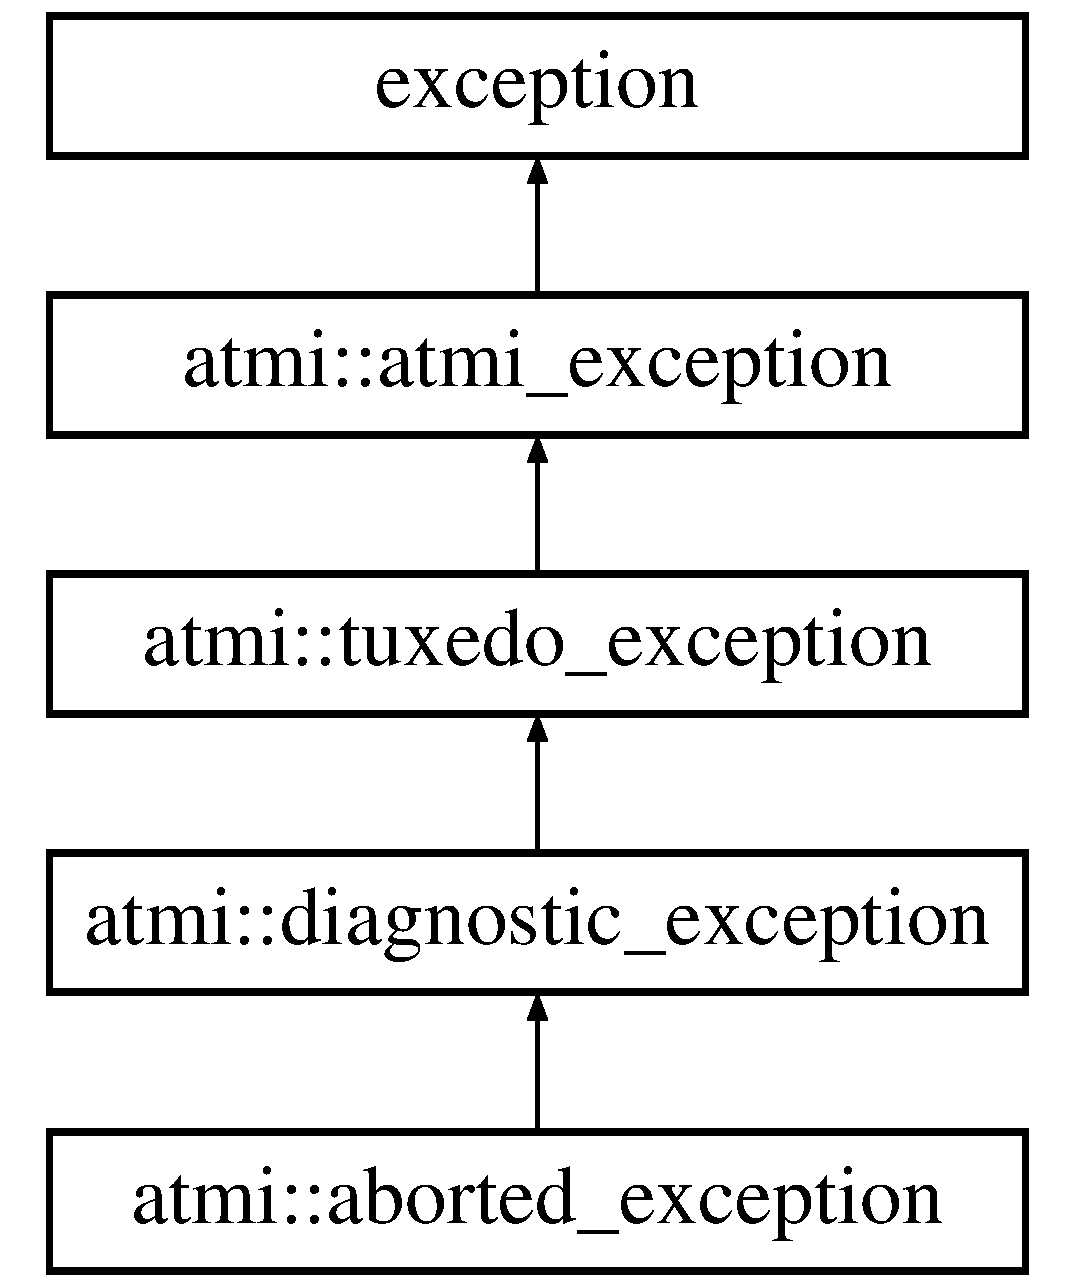
\includegraphics[height=5.000000cm]{classatmi_1_1aborted__exception}
\end{center}
\end{figure}
\subsection*{Public Member Functions}
\begin{DoxyCompactItemize}
\item 
{\footnotesize template$<$typename... Args$>$ }\\\hyperlink{classatmi_1_1aborted__exception_ab2a2defdbafa60f2566c55a078bc502a}{aborted\+\_\+exception} (const char $\ast$msg, const Args \&...args)
\end{DoxyCompactItemize}
\subsection*{Additional Inherited Members}


\subsection{Detailed Description}
Thrown when Q\+M\+E\+A\+B\+O\+R\+T\+E\+D is returned 

\subsection{Constructor \& Destructor Documentation}
\hypertarget{classatmi_1_1aborted__exception_ab2a2defdbafa60f2566c55a078bc502a}{}\index{atmi\+::aborted\+\_\+exception@{atmi\+::aborted\+\_\+exception}!aborted\+\_\+exception@{aborted\+\_\+exception}}
\index{aborted\+\_\+exception@{aborted\+\_\+exception}!atmi\+::aborted\+\_\+exception@{atmi\+::aborted\+\_\+exception}}
\subsubsection[{aborted\+\_\+exception(const char $\ast$msg, const Args \&...\+args)}]{\setlength{\rightskip}{0pt plus 5cm}template$<$typename... Args$>$ atmi\+::aborted\+\_\+exception\+::aborted\+\_\+exception (
\begin{DoxyParamCaption}
\item[{const char $\ast$}]{msg, }
\item[{const Args \&...}]{args}
\end{DoxyParamCaption}
)\hspace{0.3cm}{\ttfamily [inline]}}\label{classatmi_1_1aborted__exception_ab2a2defdbafa60f2566c55a078bc502a}
Constructs an aborted exeption


\begin{DoxyParams}{Parameters}
{\em err} & value of tperr \\
\hline
{\em diagno} & value of ctl.\+diagnostic \\
\hline
{\em msg} & error message format. \\
\hline
{\em args} & error message parameters \\
\hline
\end{DoxyParams}


The documentation for this class was generated from the following file\+:\begin{DoxyCompactItemize}
\item 
include/atmi/exceptions.\+hpp\end{DoxyCompactItemize}

\hypertarget{classatmi_1_1abstract__client}{}\section{atmi\+:\+:abstract\+\_\+client Class Reference}
\label{classatmi_1_1abstract__client}\index{atmi\+::abstract\+\_\+client@{atmi\+::abstract\+\_\+client}}


{\ttfamily \#include $<$tuxedo.\+hpp$>$}

Inheritance diagram for atmi\+:\+:abstract\+\_\+client\+:\begin{figure}[H]
\begin{center}
\leavevmode
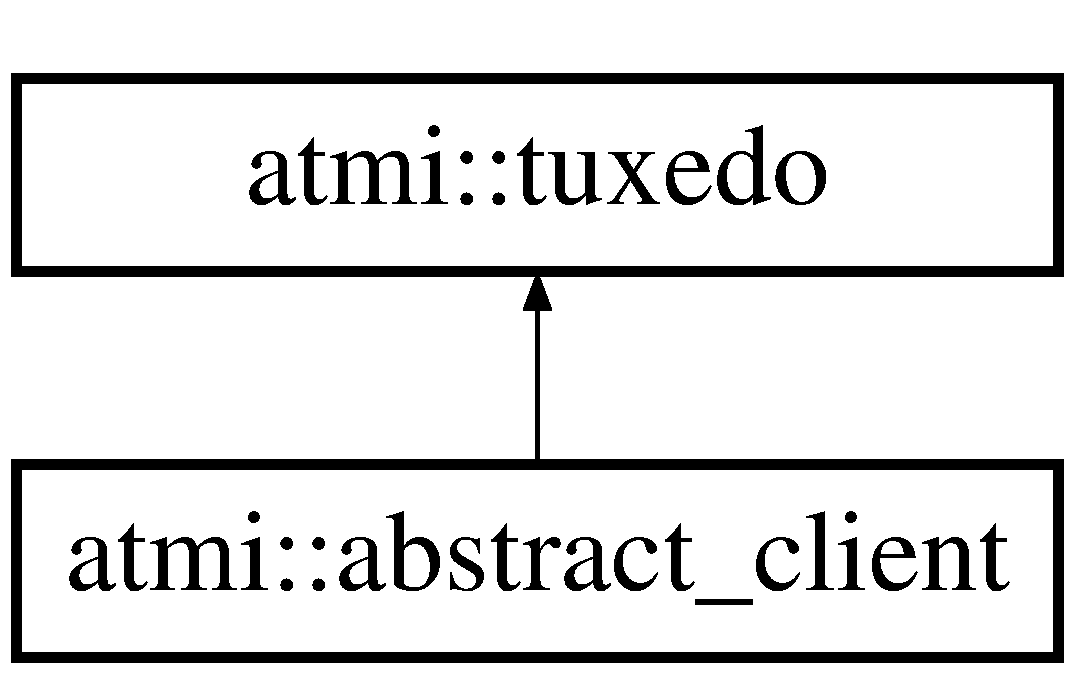
\includegraphics[height=2.000000cm]{classatmi_1_1abstract__client}
\end{center}
\end{figure}
\subsection*{Public Member Functions}
\begin{DoxyCompactItemize}
\item 
virtual \hyperlink{classatmi_1_1abstract__client_a789a662f195c11cd9d9b6d091caa0874}{$\sim$abstract\+\_\+client} ()
\item 
\hyperlink{classatmi_1_1abstract__client_a10a6aa2b44cb98ceab7d4e637757437e}{abstract\+\_\+client} ()
\item 
\hyperlink{classatmi_1_1abstract__client_a67d65b7ec70b83b7fc55260256ac4fd0}{abstract\+\_\+client} (const char $\ast$cltname, const char $\ast$usr=N\+U\+L\+L, const char $\ast$passwd=N\+U\+L\+L, const char $\ast$group=N\+U\+L\+L, const char $\ast$\hyperlink{classatmi_1_1abstract__client_af2a6efcd7a45c09251cb129d04d7aa85}{tuxconfig}=N\+U\+L\+L)
\item 
virtual int \hyperlink{classatmi_1_1abstract__client_a090bac30edb1055da2a0c980167bfe19}{run} (int argc, char $\ast$$\ast$argv)
\item 
\hyperlink{group__atmi_gafc1ae4cdb2829f98c37f27b472fcb867}{transaction\+\_\+ptr} \hyperlink{classatmi_1_1abstract__client_a9449f2df2136afd5b253389418265c87}{new\+\_\+transaction\+\_\+instance} (const char $\ast$svc)
\item 
\hyperlink{group__atmi_gaf8c3e342d908ddc295b73c376b7515ca}{queue\+\_\+ptr} \hyperlink{classatmi_1_1abstract__client_a7337c966369376497d9c1f94ec12c5ae}{new\+\_\+queue\+\_\+instance} (const char $\ast$qspace, const char $\ast$\hyperlink{classatmi_1_1queue}{queue}, const char $\ast$reply=N\+U\+L\+L)
\item 
const char $\ast$ \hyperlink{classatmi_1_1abstract__client_a2f50ed746c5bab5e01ef0677296e10e3}{name} () const 
\item 
const char $\ast$ \hyperlink{classatmi_1_1abstract__client_af2a6efcd7a45c09251cb129d04d7aa85}{tuxconfig} () const 
\item 
bool \hyperlink{classatmi_1_1abstract__client_a026c8cff81a66afdcfa3bf977417738a}{multi\+\_\+context} ()
\end{DoxyCompactItemize}
\subsection*{Additional Inherited Members}


\subsection{Detailed Description}
Helper class to implement tuxedo application.

Extending this class ensures that tpterm and tpinit is called when client programs are run.

\hyperlink{classatmi_1_1abstract__client}{abstract\+\_\+client} has two modes of operation\+: single-\/context mode and multicontext mode. To run in multicontext mode you\textquotesingle{}ll need to pass a valid T\+U\+X\+C\+O\+N\+F\+I\+G file when constructing an \hyperlink{classatmi_1_1abstract__client}{abstract\+\_\+client} instance. The multiconext mode is available only for native clients.

Two factory methods are available to construct transaction and queue class instances (new\+\_\+tp\+\_\+instance and new\+\_\+queue\+\_\+instance). These methods return tp\+\_\+auto\+\_\+ptr and queue\+\_\+auto\+\_\+ptr which are auto pointers. which is probaly the best way to avoid memory leaks. 

\subsection{Constructor \& Destructor Documentation}
\hypertarget{classatmi_1_1abstract__client_a789a662f195c11cd9d9b6d091caa0874}{}\index{atmi\+::abstract\+\_\+client@{atmi\+::abstract\+\_\+client}!````~abstract\+\_\+client@{$\sim$abstract\+\_\+client}}
\index{````~abstract\+\_\+client@{$\sim$abstract\+\_\+client}!atmi\+::abstract\+\_\+client@{atmi\+::abstract\+\_\+client}}
\subsubsection[{$\sim$abstract\+\_\+client()}]{\setlength{\rightskip}{0pt plus 5cm}atmi\+::abstract\+\_\+client\+::$\sim$abstract\+\_\+client (
\begin{DoxyParamCaption}
{}
\end{DoxyParamCaption}
)\hspace{0.3cm}{\ttfamily [virtual]}}\label{classatmi_1_1abstract__client_a789a662f195c11cd9d9b6d091caa0874}
Method moved into the destructor of \hyperlink{classatmi_1_1abstract__client}{abstract\+\_\+client} End any pending operation and free any alloated ressource. After this call any attempt at using A\+T\+M\+I will fail. int term () ; \hypertarget{classatmi_1_1abstract__client_a10a6aa2b44cb98ceab7d4e637757437e}{}\index{atmi\+::abstract\+\_\+client@{atmi\+::abstract\+\_\+client}!abstract\+\_\+client@{abstract\+\_\+client}}
\index{abstract\+\_\+client@{abstract\+\_\+client}!atmi\+::abstract\+\_\+client@{atmi\+::abstract\+\_\+client}}
\subsubsection[{abstract\+\_\+client()}]{\setlength{\rightskip}{0pt plus 5cm}atmi\+::abstract\+\_\+client\+::abstract\+\_\+client (
\begin{DoxyParamCaption}
{}
\end{DoxyParamCaption}
)}\label{classatmi_1_1abstract__client_a10a6aa2b44cb98ceab7d4e637757437e}
Join a B\+E\+A tuxedo A\+T\+M\+I system application by calling tpinit.

Before a client can use any of the B\+E\+A tuxedo A\+T\+M\+I system communication or transaction routines, it must first join a B\+E\+A tuxedo A\+T\+M\+I system application by explicitly using tpinit. \hypertarget{classatmi_1_1abstract__client_a67d65b7ec70b83b7fc55260256ac4fd0}{}\index{atmi\+::abstract\+\_\+client@{atmi\+::abstract\+\_\+client}!abstract\+\_\+client@{abstract\+\_\+client}}
\index{abstract\+\_\+client@{abstract\+\_\+client}!atmi\+::abstract\+\_\+client@{atmi\+::abstract\+\_\+client}}
\subsubsection[{abstract\+\_\+client(const char $\ast$cltname, const char $\ast$usr=\+N\+U\+L\+L, const char $\ast$passwd=\+N\+U\+L\+L, const char $\ast$group=\+N\+U\+L\+L, const char $\ast$tuxconfig=\+N\+U\+L\+L)}]{\setlength{\rightskip}{0pt plus 5cm}atmi\+::abstract\+\_\+client\+::abstract\+\_\+client (
\begin{DoxyParamCaption}
\item[{const char $\ast$}]{cltname, }
\item[{const char $\ast$}]{usr = {\ttfamily NULL}, }
\item[{const char $\ast$}]{passwd = {\ttfamily NULL}, }
\item[{const char $\ast$}]{group = {\ttfamily NULL}, }
\item[{const char $\ast$}]{tuxconfig = {\ttfamily NULL}}
\end{DoxyParamCaption}
)}\label{classatmi_1_1abstract__client_a67d65b7ec70b83b7fc55260256ac4fd0}
Join a B\+E\+A tuxedo A\+T\+M\+I system application by calling tpinit.

This constructor sets the T\+P\+I\+N\+F\+O flag T\+P\+M\+U\+L\+T\+I\+C\+O\+N\+T\+E\+X\+T\+S.

In a multi threaded application it is good practice to initiliaze all your clients before starting the threads or to use a factory.

Before a client can use any of the B\+E\+A tuxedo A\+T\+M\+I system communication or transaction routines, it must first join a B\+E\+A tuxedo A\+T\+M\+I system application by explicitly using tpinit.

If passwd is N\+U\+L\+L then the constructor checks if authentication is needed. If so it promps the user for a password.


\begin{DoxyParams}{Parameters}
{\em cltname} & client program name (default N\+U\+L\+L) \\
\hline
{\em usr} & user name (default N\+U\+L\+L) \\
\hline
{\em passwd} & user\textquotesingle{}s password (default N\+U\+L\+L) \\
\hline
{\em group} & is used to associate the client with a resource manager group name (default N\+U\+L\+L) \\
\hline
{\em tuxconfig} & used located the D\+O\+M\+A\+I\+N \\
\hline
\end{DoxyParams}


\subsection{Member Function Documentation}
\hypertarget{classatmi_1_1abstract__client_a026c8cff81a66afdcfa3bf977417738a}{}\index{atmi\+::abstract\+\_\+client@{atmi\+::abstract\+\_\+client}!multi\+\_\+context@{multi\+\_\+context}}
\index{multi\+\_\+context@{multi\+\_\+context}!atmi\+::abstract\+\_\+client@{atmi\+::abstract\+\_\+client}}
\subsubsection[{multi\+\_\+context()}]{\setlength{\rightskip}{0pt plus 5cm}bool atmi\+::abstract\+\_\+client\+::multi\+\_\+context (
\begin{DoxyParamCaption}
{}
\end{DoxyParamCaption}
)\hspace{0.3cm}{\ttfamily [inline]}}\label{classatmi_1_1abstract__client_a026c8cff81a66afdcfa3bf977417738a}
\begin{DoxyReturn}{Returns}
true if multicontext is active 
\end{DoxyReturn}
\hypertarget{classatmi_1_1abstract__client_a2f50ed746c5bab5e01ef0677296e10e3}{}\index{atmi\+::abstract\+\_\+client@{atmi\+::abstract\+\_\+client}!name@{name}}
\index{name@{name}!atmi\+::abstract\+\_\+client@{atmi\+::abstract\+\_\+client}}
\subsubsection[{name() const }]{\setlength{\rightskip}{0pt plus 5cm}const char$\ast$ atmi\+::abstract\+\_\+client\+::name (
\begin{DoxyParamCaption}
{}
\end{DoxyParamCaption}
) const\hspace{0.3cm}{\ttfamily [inline]}}\label{classatmi_1_1abstract__client_a2f50ed746c5bab5e01ef0677296e10e3}
\begin{DoxyReturn}{Returns}
tuxedo client name 
\end{DoxyReturn}
\hypertarget{classatmi_1_1abstract__client_a7337c966369376497d9c1f94ec12c5ae}{}\index{atmi\+::abstract\+\_\+client@{atmi\+::abstract\+\_\+client}!new\+\_\+queue\+\_\+instance@{new\+\_\+queue\+\_\+instance}}
\index{new\+\_\+queue\+\_\+instance@{new\+\_\+queue\+\_\+instance}!atmi\+::abstract\+\_\+client@{atmi\+::abstract\+\_\+client}}
\subsubsection[{new\+\_\+queue\+\_\+instance(const char $\ast$qspace, const char $\ast$queue, const char $\ast$reply=\+N\+U\+L\+L)}]{\setlength{\rightskip}{0pt plus 5cm}{\bf queue\+\_\+ptr} atmi\+::abstract\+\_\+client\+::new\+\_\+queue\+\_\+instance (
\begin{DoxyParamCaption}
\item[{const char $\ast$}]{qspace, }
\item[{const char $\ast$}]{queue, }
\item[{const char $\ast$}]{reply = {\ttfamily NULL}}
\end{DoxyParamCaption}
)}\label{classatmi_1_1abstract__client_a7337c966369376497d9c1f94ec12c5ae}
Creates an instance of queue and set the client context to be used.

\begin{DoxyReturn}{Returns}
an auto\+\_\+ptr to a new queue instance 
\end{DoxyReturn}
\hypertarget{classatmi_1_1abstract__client_a9449f2df2136afd5b253389418265c87}{}\index{atmi\+::abstract\+\_\+client@{atmi\+::abstract\+\_\+client}!new\+\_\+transaction\+\_\+instance@{new\+\_\+transaction\+\_\+instance}}
\index{new\+\_\+transaction\+\_\+instance@{new\+\_\+transaction\+\_\+instance}!atmi\+::abstract\+\_\+client@{atmi\+::abstract\+\_\+client}}
\subsubsection[{new\+\_\+transaction\+\_\+instance(const char $\ast$svc)}]{\setlength{\rightskip}{0pt plus 5cm}{\bf transaction\+\_\+ptr} atmi\+::abstract\+\_\+client\+::new\+\_\+transaction\+\_\+instance (
\begin{DoxyParamCaption}
\item[{const char $\ast$}]{svc}
\end{DoxyParamCaption}
)}\label{classatmi_1_1abstract__client_a9449f2df2136afd5b253389418265c87}
Creates an instance of transaction and set the client context to be used.

\begin{DoxyReturn}{Returns}
an auto\+\_\+ptr to a new transaction instance 
\end{DoxyReturn}
\hypertarget{classatmi_1_1abstract__client_a090bac30edb1055da2a0c980167bfe19}{}\index{atmi\+::abstract\+\_\+client@{atmi\+::abstract\+\_\+client}!run@{run}}
\index{run@{run}!atmi\+::abstract\+\_\+client@{atmi\+::abstract\+\_\+client}}
\subsubsection[{run(int argc, char $\ast$$\ast$argv)}]{\setlength{\rightskip}{0pt plus 5cm}virtual int atmi\+::abstract\+\_\+client\+::run (
\begin{DoxyParamCaption}
\item[{int}]{argc, }
\item[{char $\ast$$\ast$}]{argv}
\end{DoxyParamCaption}
)\hspace{0.3cm}{\ttfamily [inline]}, {\ttfamily [virtual]}}\label{classatmi_1_1abstract__client_a090bac30edb1055da2a0c980167bfe19}
This method must overriden to run the client application.


\begin{DoxyParams}{Parameters}
{\em argc} & number of command line option received when the program was started \\
\hline
{\em argv} & actual value of command line arguments \\
\hline
\end{DoxyParams}
\begin{DoxyRefDesc}{Deprecated}
\item[\hyperlink{deprecated__deprecated000007}{Deprecated}]\end{DoxyRefDesc}
\hypertarget{classatmi_1_1abstract__client_af2a6efcd7a45c09251cb129d04d7aa85}{}\index{atmi\+::abstract\+\_\+client@{atmi\+::abstract\+\_\+client}!tuxconfig@{tuxconfig}}
\index{tuxconfig@{tuxconfig}!atmi\+::abstract\+\_\+client@{atmi\+::abstract\+\_\+client}}
\subsubsection[{tuxconfig() const }]{\setlength{\rightskip}{0pt plus 5cm}const char$\ast$ atmi\+::abstract\+\_\+client\+::tuxconfig (
\begin{DoxyParamCaption}
{}
\end{DoxyParamCaption}
) const\hspace{0.3cm}{\ttfamily [inline]}}\label{classatmi_1_1abstract__client_af2a6efcd7a45c09251cb129d04d7aa85}
\begin{DoxyReturn}{Returns}
associated T\+U\+X\+C\+O\+N\+F\+I\+G value 
\end{DoxyReturn}


The documentation for this class was generated from the following files\+:\begin{DoxyCompactItemize}
\item 
include/atmi/tuxedo.\+hpp\item 
src/abstract\+\_\+client.\+cpp\end{DoxyCompactItemize}

\hypertarget{classatmi_1_1atmi__exception}{}\section{atmi\+:\+:atmi\+\_\+exception Class Reference}
\label{classatmi_1_1atmi__exception}\index{atmi\+::atmi\+\_\+exception@{atmi\+::atmi\+\_\+exception}}


{\ttfamily \#include $<$exceptions.\+hpp$>$}

Inheritance diagram for atmi\+:\+:atmi\+\_\+exception\+:\begin{figure}[H]
\begin{center}
\leavevmode
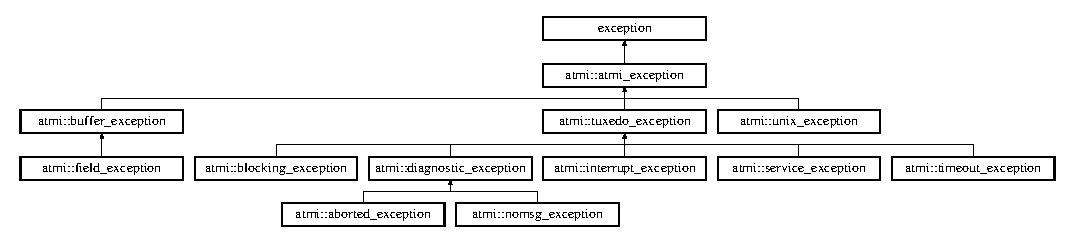
\includegraphics[height=3.373494cm]{classatmi_1_1atmi__exception}
\end{center}
\end{figure}
\subsection*{Public Member Functions}
\begin{DoxyCompactItemize}
\item 
{\footnotesize template$<$typename... Args$>$ }\\\hyperlink{classatmi_1_1atmi__exception_a95882b5a28a14774110080a50601abd5}{atmi\+\_\+exception} (const char $\ast$msg, const Args \&...args)
\item 
\hyperlink{classatmi_1_1atmi__exception_afa30faf28ecbc27a8aeb06dccd3b1de6}{atmi\+\_\+exception} ()
\item 
virtual const char $\ast$ \hyperlink{classatmi_1_1atmi__exception_ac4f376d7dc01ce853fa3f3d2d407b3a3}{what} () const  noexcept override
\item 
virtual const char $\ast$ \hyperlink{classatmi_1_1atmi__exception_a4d457a0e0ced6177ce86a241691c8239}{message} () const  noexcept
\end{DoxyCompactItemize}
\subsection*{Protected Attributes}
\begin{DoxyCompactItemize}
\item 
std\+::string \hyperlink{classatmi_1_1atmi__exception_a04aa0d2991971df8e87f68cbbbaa02b2}{\+\_\+what}\hypertarget{classatmi_1_1atmi__exception_a04aa0d2991971df8e87f68cbbbaa02b2}{}\label{classatmi_1_1atmi__exception_a04aa0d2991971df8e87f68cbbbaa02b2}

\begin{DoxyCompactList}\small\item\em what message (often the concatenation of message + other infos) \end{DoxyCompactList}\item 
std\+::string \hyperlink{classatmi_1_1atmi__exception_a709aa3b3b70930ed40d442ec7fbb6b99}{\+\_\+message}\hypertarget{classatmi_1_1atmi__exception_a709aa3b3b70930ed40d442ec7fbb6b99}{}\label{classatmi_1_1atmi__exception_a709aa3b3b70930ed40d442ec7fbb6b99}

\begin{DoxyCompactList}\small\item\em error message \end{DoxyCompactList}\end{DoxyCompactItemize}


\subsection{Detailed Description}
Base class of A\+T\+M\+I++ exception

Can be used to throw any kind of error message in a consitent way. 

\subsection{Constructor \& Destructor Documentation}
\index{atmi\+::atmi\+\_\+exception@{atmi\+::atmi\+\_\+exception}!atmi\+\_\+exception@{atmi\+\_\+exception}}
\index{atmi\+\_\+exception@{atmi\+\_\+exception}!atmi\+::atmi\+\_\+exception@{atmi\+::atmi\+\_\+exception}}
\subsubsection[{\texorpdfstring{atmi\+\_\+exception(const char $\ast$msg, const Args \&...\+args)}{atmi\_exception(const char *msg, const Args \&...args)}}]{\setlength{\rightskip}{0pt plus 5cm}template$<$typename... Args$>$ atmi\+::atmi\+\_\+exception\+::atmi\+\_\+exception (
\begin{DoxyParamCaption}
\item[{const char $\ast$}]{msg, }
\item[{const Args \&...}]{args}
\end{DoxyParamCaption}
)\hspace{0.3cm}{\ttfamily [inline]}}\hypertarget{classatmi_1_1atmi__exception_a95882b5a28a14774110080a50601abd5}{}\label{classatmi_1_1atmi__exception_a95882b5a28a14774110080a50601abd5}
create a new instance


\begin{DoxyParams}{Parameters}
{\em msg} & error message (used in snprintf) \\
\hline
{\em args} & message parameters \\
\hline
\end{DoxyParams}
\index{atmi\+::atmi\+\_\+exception@{atmi\+::atmi\+\_\+exception}!atmi\+\_\+exception@{atmi\+\_\+exception}}
\index{atmi\+\_\+exception@{atmi\+\_\+exception}!atmi\+::atmi\+\_\+exception@{atmi\+::atmi\+\_\+exception}}
\subsubsection[{\texorpdfstring{atmi\+\_\+exception()}{atmi\_exception()}}]{\setlength{\rightskip}{0pt plus 5cm}atmi\+::atmi\+\_\+exception\+::atmi\+\_\+exception (
\begin{DoxyParamCaption}
{}
\end{DoxyParamCaption}
)}\hypertarget{classatmi_1_1atmi__exception_afa30faf28ecbc27a8aeb06dccd3b1de6}{}\label{classatmi_1_1atmi__exception_afa30faf28ecbc27a8aeb06dccd3b1de6}
default constructor.

set a default message. 

\subsection{Member Function Documentation}
\index{atmi\+::atmi\+\_\+exception@{atmi\+::atmi\+\_\+exception}!message@{message}}
\index{message@{message}!atmi\+::atmi\+\_\+exception@{atmi\+::atmi\+\_\+exception}}
\subsubsection[{\texorpdfstring{message() const  noexcept}{message() const  noexcept}}]{\setlength{\rightskip}{0pt plus 5cm}const char $\ast$ atmi\+::atmi\+\_\+exception\+::message (
\begin{DoxyParamCaption}
{}
\end{DoxyParamCaption}
) const\hspace{0.3cm}{\ttfamily [virtual]}, {\ttfamily [noexcept]}}\hypertarget{classatmi_1_1atmi__exception_a4d457a0e0ced6177ce86a241691c8239}{}\label{classatmi_1_1atmi__exception_a4d457a0e0ced6177ce86a241691c8239}
\begin{DoxyReturn}{Returns}
explanatory error message. 
\end{DoxyReturn}
\index{atmi\+::atmi\+\_\+exception@{atmi\+::atmi\+\_\+exception}!what@{what}}
\index{what@{what}!atmi\+::atmi\+\_\+exception@{atmi\+::atmi\+\_\+exception}}
\subsubsection[{\texorpdfstring{what() const  noexcept override}{what() const  noexcept override}}]{\setlength{\rightskip}{0pt plus 5cm}const char $\ast$ atmi\+::atmi\+\_\+exception\+::what (
\begin{DoxyParamCaption}
{}
\end{DoxyParamCaption}
) const\hspace{0.3cm}{\ttfamily [override]}, {\ttfamily [virtual]}, {\ttfamily [noexcept]}}\hypertarget{classatmi_1_1atmi__exception_ac4f376d7dc01ce853fa3f3d2d407b3a3}{}\label{classatmi_1_1atmi__exception_ac4f376d7dc01ce853fa3f3d2d407b3a3}
\begin{DoxyReturn}{Returns}
user friendly text message 
\end{DoxyReturn}


The documentation for this class was generated from the following files\+:\begin{DoxyCompactItemize}
\item 
include/atmi/exceptions.\+hpp\item 
src/exceptions.\+cpp\end{DoxyCompactItemize}

\hypertarget{classatmi_1_1blocking__exception}{\section{atmi\+:\+:blocking\+\_\+exception Class Reference}
\label{classatmi_1_1blocking__exception}\index{atmi\+::blocking\+\_\+exception@{atmi\+::blocking\+\_\+exception}}
}


{\ttfamily \#include $<$exceptions.\+hpp$>$}

Inheritance diagram for atmi\+:\+:blocking\+\_\+exception\+:\begin{figure}[H]
\begin{center}
\leavevmode
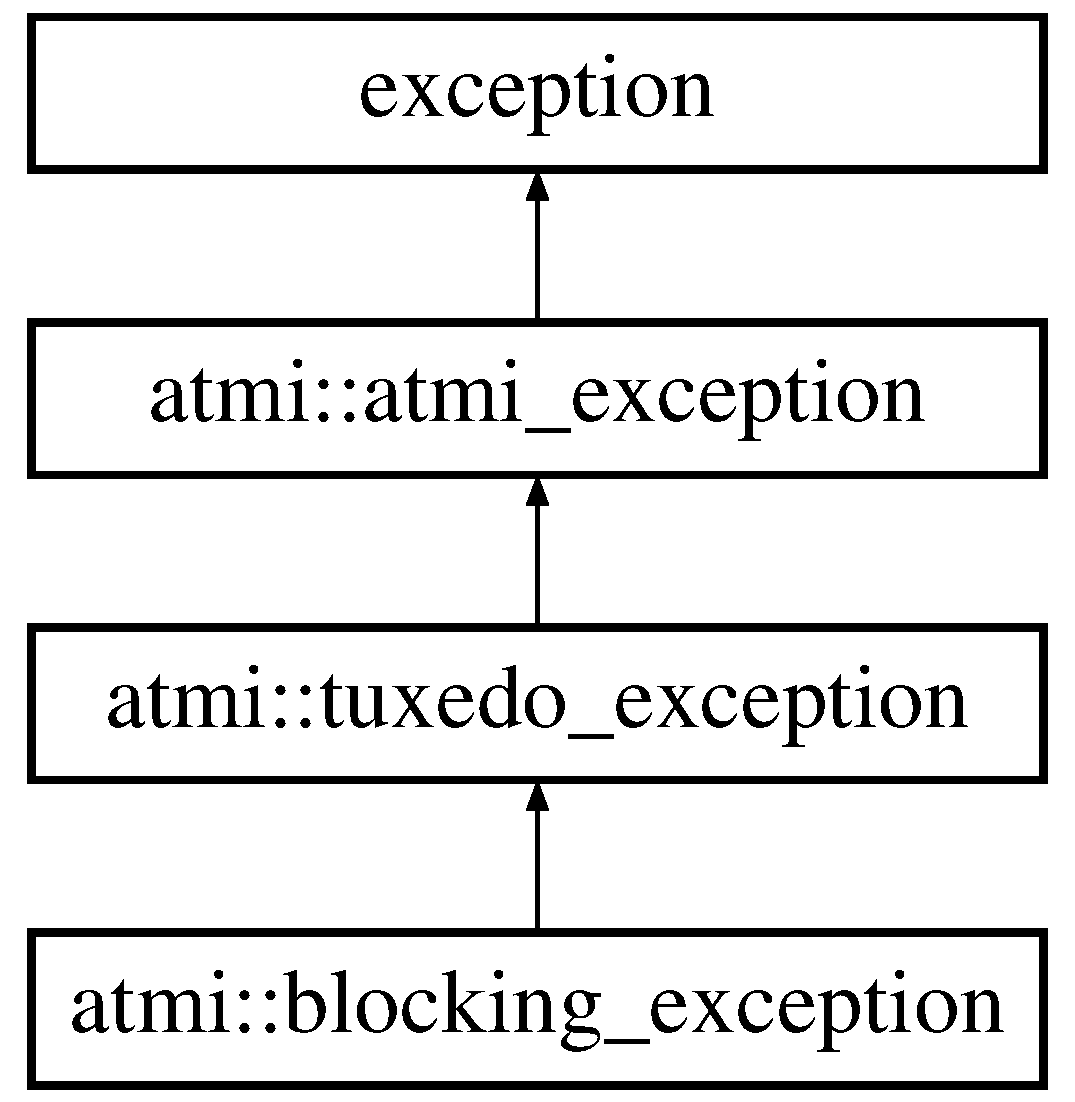
\includegraphics[height=4.000000cm]{classatmi_1_1blocking__exception}
\end{center}
\end{figure}
\subsection*{Public Member Functions}
\begin{DoxyCompactItemize}
\item 
{\footnotesize template$<$typename... Args$>$ }\\\hyperlink{classatmi_1_1blocking__exception_a2237c2b5b3264745e145d0e4e26838ad}{blocking\+\_\+exception} (const char $\ast$msg, const Args \&...args)
\end{DoxyCompactItemize}
\subsection*{Additional Inherited Members}


\subsection{Detailed Description}
Thrown when a blocking condition is detected (T\+P\+E\+B\+L\+O\+C\+K . 

\subsection{Constructor \& Destructor Documentation}
\hypertarget{classatmi_1_1blocking__exception_a2237c2b5b3264745e145d0e4e26838ad}{\index{atmi\+::blocking\+\_\+exception@{atmi\+::blocking\+\_\+exception}!blocking\+\_\+exception@{blocking\+\_\+exception}}
\index{blocking\+\_\+exception@{blocking\+\_\+exception}!atmi\+::blocking\+\_\+exception@{atmi\+::blocking\+\_\+exception}}
\subsubsection[{blocking\+\_\+exception}]{\setlength{\rightskip}{0pt plus 5cm}template$<$typename... Args$>$ atmi\+::blocking\+\_\+exception\+::blocking\+\_\+exception (
\begin{DoxyParamCaption}
\item[{const char $\ast$}]{msg, }
\item[{const Args \&...}]{args}
\end{DoxyParamCaption}
)\hspace{0.3cm}{\ttfamily [inline]}}}\label{classatmi_1_1blocking__exception_a2237c2b5b3264745e145d0e4e26838ad}
new instance.


\begin{DoxyParams}{Parameters}
{\em msg} & error message \\
\hline
{\em args} & error message parameters (variadic). \\
\hline
\end{DoxyParams}


The documentation for this class was generated from the following file\+:\begin{DoxyCompactItemize}
\item 
include/atmi/exceptions.\+hpp\end{DoxyCompactItemize}

\hypertarget{classatmi_1_1buffer}{\section{atmi\+:\+:buffer Class Reference}
\label{classatmi_1_1buffer}\index{atmi\+::buffer@{atmi\+::buffer}}
}
Inheritance diagram for atmi\+:\+:buffer\+:\begin{figure}[H]
\begin{center}
\leavevmode
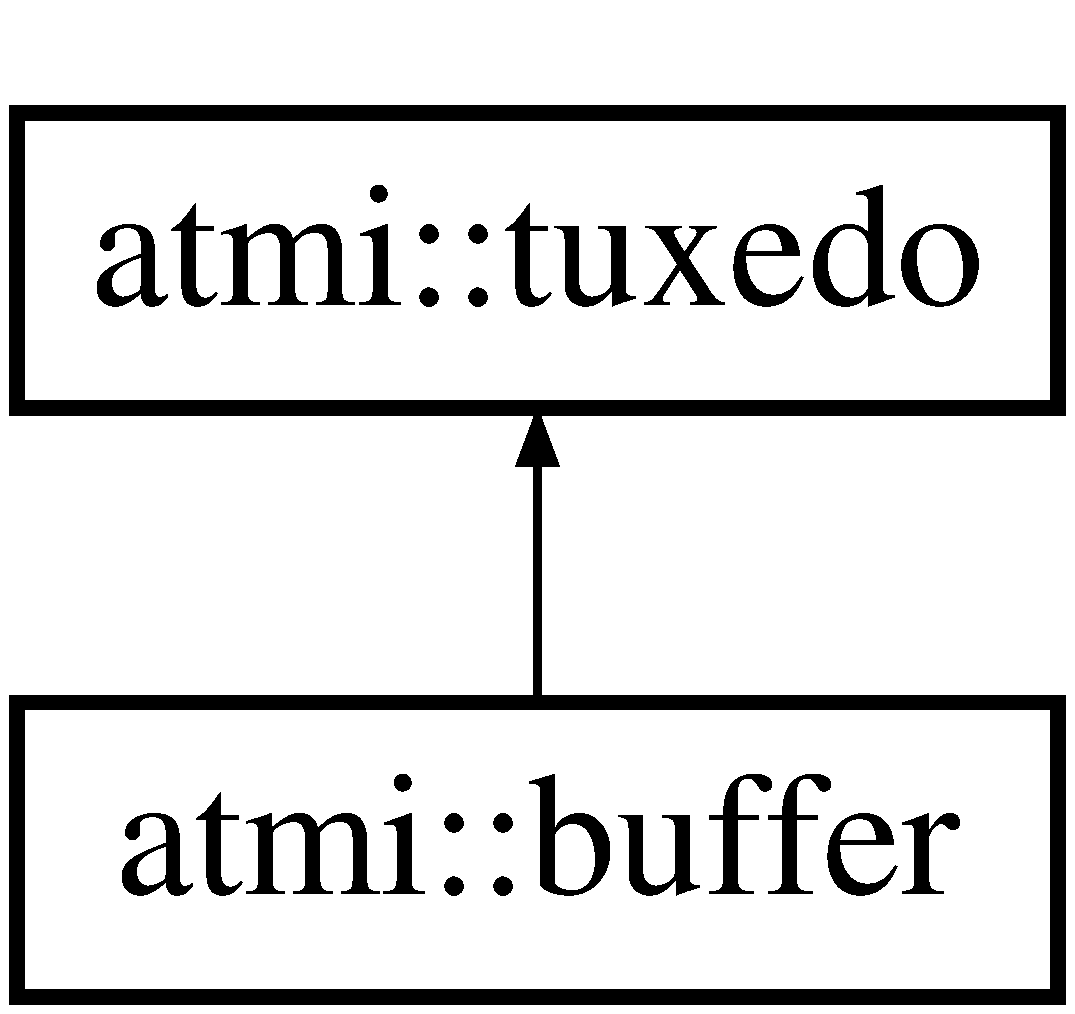
\includegraphics[height=2.000000cm]{classatmi_1_1buffer}
\end{center}
\end{figure}
\subsection*{Public Member Functions}
\begin{DoxyCompactItemize}
\item 
\hyperlink{classatmi_1_1buffer_ab5a434d367c856f9b1b7c831b98ff0d3}{buffer} ()
\item 
\hyperlink{classatmi_1_1buffer_a5a2836413da6d30d25afa2ea242cd90d}{buffer} (F\+B\+F\+R32 $\ast$b)
\item 
\hyperlink{classatmi_1_1buffer_ae2bc183e6b0909b8155dcfa17686a574}{buffer} (F\+L\+D\+L\+E\+N32 len)
\item 
\hyperlink{classatmi_1_1buffer_aa58097eacc94f1f5cc5e99b434ec7135}{$\sim$buffer} ()
\item 
void \hyperlink{classatmi_1_1buffer_a51d14f5d63ae22666ce0d5dc46e91728}{set\+\_\+call\+\_\+info} (\hyperlink{classatmi_1_1call__info}{call\+\_\+info} \&callinfo)
\item 
void \hyperlink{classatmi_1_1buffer_a84a4bd3782f9ffafa962a2393484b0b7}{get\+\_\+call\+\_\+info} (\hyperlink{classatmi_1_1call__info}{call\+\_\+info} \&callinfo)
\item 
size\+\_\+t \hyperlink{classatmi_1_1buffer_a8228f64305e566b8133e8ee746c6d2bb}{size} () const 
\item 
size\+\_\+t \hyperlink{classatmi_1_1buffer_a4ab660c5750cb0793eb99782fd36c0fa}{used} () const 
\item 
size\+\_\+t \hyperlink{classatmi_1_1buffer_a30b054d9d60238f34463d4bcd5ac3e16}{unused} () const 
\item 
void \hyperlink{classatmi_1_1buffer_ab9294b1a1e54e35717db40cb6bbb6de1}{pack} ()
\item 
void \hyperlink{classatmi_1_1buffer_a853e2a0585dda4e23ffa04297b824afb}{extend} ()
\item 
size\+\_\+t \hyperlink{classatmi_1_1buffer_af35cd2e5a5cdd7499fb396dbdbe3f61a}{extent} () const 
\item 
void \hyperlink{classatmi_1_1buffer_a10150940e8fc679b6bdc52bc02e6d016}{set\+\_\+extent} (size\+\_\+t \hyperlink{classatmi_1_1buffer_af35cd2e5a5cdd7499fb396dbdbe3f61a}{extent})
\item 
void \hyperlink{classatmi_1_1buffer_a95d13597c2f28bfc8ee5dac4db131179}{resize} (size\+\_\+t \hyperlink{classatmi_1_1buffer_af35cd2e5a5cdd7499fb396dbdbe3f61a}{extent})
\item 
\hyperlink{classatmi_1_1field}{field} \& \hyperlink{classatmi_1_1buffer_a1fe98844cb17328390b3d4e658bd6903}{set} (\hyperlink{classatmi_1_1field}{field} \&f)
\item 
\hyperlink{classatmi_1_1field}{field} \& \hyperlink{classatmi_1_1buffer_a5f30826d8273b619380e8b4f039af094}{add} (\hyperlink{classatmi_1_1field}{field} \&f)
\item 
\hyperlink{classatmi_1_1field}{field} \& \hyperlink{classatmi_1_1buffer_a4a9abeb69354fa575c8b27c9af170e79}{append} (\hyperlink{classatmi_1_1field}{field} \&f)
\item 
void \hyperlink{classatmi_1_1buffer_a4a1ef484befbf22aca919fc1a312ab61}{remove} (\hyperlink{classatmi_1_1field}{field} \&f)
\item 
\hyperlink{classatmi_1_1field}{field} \& \hyperlink{classatmi_1_1buffer_affb14c05bc21e29c3a2f6dc03c30c0fa}{get} (\hyperlink{classatmi_1_1field}{field} \&f)
\item 
\hyperlink{classatmi_1_1field}{field} \& \hyperlink{classatmi_1_1buffer_a864adb4d0153e6be38a7905c994915e1}{get} (\hyperlink{classatmi_1_1field}{field} \&f, F\+L\+D\+O\+C\+C32 occ)
\item 
long \hyperlink{classatmi_1_1buffer_a4ae9fa419098eb136ae3681ad90ccafb}{chksum} ()
\item 
F\+L\+D\+O\+C\+C32 \hyperlink{classatmi_1_1buffer_a57ff1b2ed449d59d4ec936e9e79a5d1a}{occurences} (const \hyperlink{classatmi_1_1field}{field} \&f)
\item 
F\+L\+D\+O\+C\+C32 \hyperlink{classatmi_1_1buffer_a74a6ff6ab31eb1128fc2f40d2a8e020f}{field\+\_\+count} () const 
\item 
size\+\_\+t \hyperlink{classatmi_1_1buffer_ae315c028b78f321abce6d9be2e026813}{print\+\_\+buffer\+\_\+size} () const 
\item 
void \hyperlink{classatmi_1_1buffer_ad7b1a3f9005926e07d00393aa6300f39}{print} (char $\ast$\hyperlink{classatmi_1_1buffer}{buffer}) const 
\item 
void \hyperlink{classatmi_1_1buffer_aa5f087559f5f3fb4f383121f78f2c461}{print} () const 
\item 
F\+B\+F\+R32 $\ast$ \hyperlink{classatmi_1_1buffer_aa9aa5382717ed17a2047db2779f8f0ec}{get\+\_\+buffer} ()
\item 
void \hyperlink{classatmi_1_1buffer_ade8853e7c2ae10dcd024b34049e99af3}{set\+\_\+buffer} (F\+B\+F\+R32 $\ast$b)
\item 
bool \hyperlink{classatmi_1_1buffer_aae543cf7816b338d20031993c18ce491}{is\+\_\+handling\+\_\+memory} ()
\item 
void \hyperlink{classatmi_1_1buffer_a68f05d1dbd040062850feeba5aa188fc}{set\+\_\+handling\+\_\+memory} (bool b)
\item 
\hyperlink{classatmi_1_1buffer_a79e82bc3f9dac86efc685604c20ed78d}{operator F\+B\+F\+R32 $\ast$} ()
\item 
bool \hyperlink{classatmi_1_1buffer_aa095219e6aa1470c96dc2b3d4ddeeb98}{operator==} (\hyperlink{classatmi_1_1buffer}{buffer} \&b)
\item 
\hyperlink{classatmi_1_1buffer}{buffer} \& \hyperlink{classatmi_1_1buffer_a878220e2ba9a66a991c77b20fd52ff09}{operator=} (\hyperlink{classatmi_1_1buffer}{buffer} \&b)
\item 
\hyperlink{classatmi_1_1buffer}{buffer} \& \hyperlink{classatmi_1_1buffer_a4efc77b0773f85c06d391af8a7ebe98a}{operator=} (F\+B\+F\+R32 $\ast$b)
\end{DoxyCompactItemize}
\subsection*{Static Public Member Functions}
\begin{DoxyCompactItemize}
\item 
static bool \hyperlink{classatmi_1_1buffer_a38aca9956db23474cb19d4c737b08262}{is\+\_\+fml32\+\_\+buffer} (char $\ast$\hyperlink{classatmi_1_1buffer}{buffer})
\end{DoxyCompactItemize}
\subsection*{Friends}
\begin{DoxyCompactItemize}
\item 
\hypertarget{classatmi_1_1buffer_acd53905ae10cba58b4337aefe648aec6}{class {\bfseries field}}\label{classatmi_1_1buffer_acd53905ae10cba58b4337aefe648aec6}

\end{DoxyCompactItemize}
\subsection*{Additional Inherited Members}


\subsection{Constructor \& Destructor Documentation}
\hypertarget{classatmi_1_1buffer_ab5a434d367c856f9b1b7c831b98ff0d3}{\index{atmi\+::buffer@{atmi\+::buffer}!buffer@{buffer}}
\index{buffer@{buffer}!atmi\+::buffer@{atmi\+::buffer}}
\subsubsection[{buffer}]{\setlength{\rightskip}{0pt plus 5cm}atmi\+::buffer\+::buffer (
\begin{DoxyParamCaption}
{}
\end{DoxyParamCaption}
)}}\label{classatmi_1_1buffer_ab5a434d367c856f9b1b7c831b98ff0d3}
Allocates a buffer of 1024bytes \hypertarget{classatmi_1_1buffer_a5a2836413da6d30d25afa2ea242cd90d}{\index{atmi\+::buffer@{atmi\+::buffer}!buffer@{buffer}}
\index{buffer@{buffer}!atmi\+::buffer@{atmi\+::buffer}}
\subsubsection[{buffer}]{\setlength{\rightskip}{0pt plus 5cm}atmi\+::buffer\+::buffer (
\begin{DoxyParamCaption}
\item[{F\+B\+F\+R32 $\ast$}]{b}
\end{DoxyParamCaption}
)\hspace{0.3cm}{\ttfamily [explicit]}}}\label{classatmi_1_1buffer_a5a2836413da6d30d25afa2ea242cd90d}
Create a new buffer reference.

Memory allocation (alloc/free) are not handled by the instance create by this constructor. We assume that the given buffer was allocated elsewhere. And it will be deallocated later.


\begin{DoxyParams}{Parameters}
{\em b} & set F\+M\+L32 buffer reference \\
\hline
\end{DoxyParams}
\hypertarget{classatmi_1_1buffer_ae2bc183e6b0909b8155dcfa17686a574}{\index{atmi\+::buffer@{atmi\+::buffer}!buffer@{buffer}}
\index{buffer@{buffer}!atmi\+::buffer@{atmi\+::buffer}}
\subsubsection[{buffer}]{\setlength{\rightskip}{0pt plus 5cm}atmi\+::buffer\+::buffer (
\begin{DoxyParamCaption}
\item[{F\+L\+D\+L\+E\+N32}]{len}
\end{DoxyParamCaption}
)\hspace{0.3cm}{\ttfamily [explicit]}}}\label{classatmi_1_1buffer_ae2bc183e6b0909b8155dcfa17686a574}
Allocates a buffer of byte size. 
\begin{DoxyParams}{Parameters}
{\em len} & bytes space of field value in bytres \\
\hline
\end{DoxyParams}
\hypertarget{classatmi_1_1buffer_aa58097eacc94f1f5cc5e99b434ec7135}{\index{atmi\+::buffer@{atmi\+::buffer}!````~buffer@{$\sim$buffer}}
\index{````~buffer@{$\sim$buffer}!atmi\+::buffer@{atmi\+::buffer}}
\subsubsection[{$\sim$buffer}]{\setlength{\rightskip}{0pt plus 5cm}atmi\+::buffer\+::$\sim$buffer (
\begin{DoxyParamCaption}
{}
\end{DoxyParamCaption}
)}}\label{classatmi_1_1buffer_aa58097eacc94f1f5cc5e99b434ec7135}
default destructor

If memory was allocated by this instance then it will be freed. Otherwise the buffer is not deallocated. 

\subsection{Member Function Documentation}
\hypertarget{classatmi_1_1buffer_a5f30826d8273b619380e8b4f039af094}{\index{atmi\+::buffer@{atmi\+::buffer}!add@{add}}
\index{add@{add}!atmi\+::buffer@{atmi\+::buffer}}
\subsubsection[{add}]{\setlength{\rightskip}{0pt plus 5cm}{\bf field} \& atmi\+::buffer\+::add (
\begin{DoxyParamCaption}
\item[{{\bf field} \&}]{f}
\end{DoxyParamCaption}
)}}\label{classatmi_1_1buffer_a5f30826d8273b619380e8b4f039af094}
Adds a field into the buffer (Fadd32).

Adds an occurence of a field to the buffer. The first call becomes occurence 0. When successfully added the occurence property of the field is set.


\begin{DoxyParams}{Parameters}
{\em f} & a pointer to the field to add into the buffer \\
\hline
\end{DoxyParams}

\begin{DoxyExceptions}{Exceptions}
{\em \hyperlink{classatmi_1_1buffer__exception}{buffer\+\_\+exception}} & upon failure\\
\hline
\end{DoxyExceptions}
\begin{DoxySeeAlso}{See also}
\hyperlink{classatmi_1_1buffer_a1fe98844cb17328390b3d4e658bd6903}{set} to update the value of a \hyperlink{classatmi_1_1field}{field} in a \hyperlink{classatmi_1_1buffer}{buffer}
\end{DoxySeeAlso}
add the field into the buffer.


\begin{DoxyParams}{Parameters}
{\em f} & the field to add \\
\hline
\end{DoxyParams}
\hypertarget{classatmi_1_1buffer_a4a9abeb69354fa575c8b27c9af170e79}{\index{atmi\+::buffer@{atmi\+::buffer}!append@{append}}
\index{append@{append}!atmi\+::buffer@{atmi\+::buffer}}
\subsubsection[{append}]{\setlength{\rightskip}{0pt plus 5cm}{\bf field} \& atmi\+::buffer\+::append (
\begin{DoxyParamCaption}
\item[{{\bf field} \&}]{f}
\end{DoxyParamCaption}
)}}\label{classatmi_1_1buffer_a4a9abeb69354fa575c8b27c9af170e79}
Appends a field to the buffer


\begin{DoxyParams}{Parameters}
{\em f} & a pointer to the field to add into the buffer \\
\hline
\end{DoxyParams}
\begin{DoxyRefDesc}{Deprecated}
\item[\hyperlink{deprecated__deprecated000002}{Deprecated}]not implemented. \end{DoxyRefDesc}
\hypertarget{classatmi_1_1buffer_a4ae9fa419098eb136ae3681ad90ccafb}{\index{atmi\+::buffer@{atmi\+::buffer}!chksum@{chksum}}
\index{chksum@{chksum}!atmi\+::buffer@{atmi\+::buffer}}
\subsubsection[{chksum}]{\setlength{\rightskip}{0pt plus 5cm}long atmi\+::buffer\+::chksum (
\begin{DoxyParamCaption}
{}
\end{DoxyParamCaption}
)}}\label{classatmi_1_1buffer_a4ae9fa419098eb136ae3681ad90ccafb}
\begin{DoxyReturn}{Returns}
the current check sum of the buffer
\end{DoxyReturn}

\begin{DoxyExceptions}{Exceptions}
{\em \hyperlink{classatmi_1_1buffer__exception}{buffer\+\_\+exception}} & when calcutaion fails. \\
\hline
\end{DoxyExceptions}
\hypertarget{classatmi_1_1buffer_a853e2a0585dda4e23ffa04297b824afb}{\index{atmi\+::buffer@{atmi\+::buffer}!extend@{extend}}
\index{extend@{extend}!atmi\+::buffer@{atmi\+::buffer}}
\subsubsection[{extend}]{\setlength{\rightskip}{0pt plus 5cm}void atmi\+::buffer\+::extend (
\begin{DoxyParamCaption}
{}
\end{DoxyParamCaption}
)}}\label{classatmi_1_1buffer_a853e2a0585dda4e23ffa04297b824afb}
Extends the buffer size with the given bytes \hypertarget{classatmi_1_1buffer_af35cd2e5a5cdd7499fb396dbdbe3f61a}{\index{atmi\+::buffer@{atmi\+::buffer}!extent@{extent}}
\index{extent@{extent}!atmi\+::buffer@{atmi\+::buffer}}
\subsubsection[{extent}]{\setlength{\rightskip}{0pt plus 5cm}size\+\_\+t atmi\+::buffer\+::extent (
\begin{DoxyParamCaption}
{}
\end{DoxyParamCaption}
) const}}\label{classatmi_1_1buffer_af35cd2e5a5cdd7499fb396dbdbe3f61a}
\begin{DoxyReturn}{Returns}
current extent value 
\end{DoxyReturn}
\hypertarget{classatmi_1_1buffer_a74a6ff6ab31eb1128fc2f40d2a8e020f}{\index{atmi\+::buffer@{atmi\+::buffer}!field\+\_\+count@{field\+\_\+count}}
\index{field\+\_\+count@{field\+\_\+count}!atmi\+::buffer@{atmi\+::buffer}}
\subsubsection[{field\+\_\+count}]{\setlength{\rightskip}{0pt plus 5cm}F\+L\+D\+O\+C\+C32 atmi\+::buffer\+::field\+\_\+count (
\begin{DoxyParamCaption}
{}
\end{DoxyParamCaption}
) const}}\label{classatmi_1_1buffer_a74a6ff6ab31eb1128fc2f40d2a8e020f}
\begin{DoxyReturn}{Returns}
the number of fields into the buffer 
\end{DoxyReturn}
\hypertarget{classatmi_1_1buffer_affb14c05bc21e29c3a2f6dc03c30c0fa}{\index{atmi\+::buffer@{atmi\+::buffer}!get@{get}}
\index{get@{get}!atmi\+::buffer@{atmi\+::buffer}}
\subsubsection[{get}]{\setlength{\rightskip}{0pt plus 5cm}{\bf field} \& atmi\+::buffer\+::get (
\begin{DoxyParamCaption}
\item[{{\bf field} \&}]{f}
\end{DoxyParamCaption}
)}}\label{classatmi_1_1buffer_affb14c05bc21e29c3a2f6dc03c30c0fa}
Get the field value set in the buffer (Fget32).

The field's occurence property is used to find the fields value.


\begin{DoxyParams}{Parameters}
{\em f} & the field to set \\
\hline
\end{DoxyParams}
\begin{DoxyReturn}{Returns}
the field when set 
\end{DoxyReturn}

\begin{DoxyExceptions}{Exceptions}
{\em \hyperlink{classatmi_1_1buffer__exception}{buffer\+\_\+exception}} & upon failure\\
\hline
\end{DoxyExceptions}
gets the value (if exsists) of passed field


\begin{DoxyParams}{Parameters}
{\em f} & field for which we want to get the value \\
\hline
\end{DoxyParams}
\hypertarget{classatmi_1_1buffer_a864adb4d0153e6be38a7905c994915e1}{\index{atmi\+::buffer@{atmi\+::buffer}!get@{get}}
\index{get@{get}!atmi\+::buffer@{atmi\+::buffer}}
\subsubsection[{get}]{\setlength{\rightskip}{0pt plus 5cm}{\bf field} \& atmi\+::buffer\+::get (
\begin{DoxyParamCaption}
\item[{{\bf field} \&}]{f, }
\item[{F\+L\+D\+O\+C\+C32}]{occ}
\end{DoxyParamCaption}
)}}\label{classatmi_1_1buffer_a864adb4d0153e6be38a7905c994915e1}
Get the field value set in the buffer (Fget32).


\begin{DoxyParams}{Parameters}
{\em f} & the field to set \\
\hline
{\em occ} & the field occurence to set \\
\hline
\end{DoxyParams}
\begin{DoxyReturn}{Returns}
the field when set 
\end{DoxyReturn}

\begin{DoxyExceptions}{Exceptions}
{\em \hyperlink{classatmi_1_1buffer__exception}{buffer\+\_\+exception}} & upon failure\\
\hline
\end{DoxyExceptions}
gets the value (if exsists) of passed field.


\begin{DoxyParams}{Parameters}
{\em f} & field for which we want to get the value \\
\hline
\end{DoxyParams}
\hypertarget{classatmi_1_1buffer_aa9aa5382717ed17a2047db2779f8f0ec}{\index{atmi\+::buffer@{atmi\+::buffer}!get\+\_\+buffer@{get\+\_\+buffer}}
\index{get\+\_\+buffer@{get\+\_\+buffer}!atmi\+::buffer@{atmi\+::buffer}}
\subsubsection[{get\+\_\+buffer}]{\setlength{\rightskip}{0pt plus 5cm}F\+B\+F\+R32 $\ast$ atmi\+::buffer\+::get\+\_\+buffer (
\begin{DoxyParamCaption}
{}
\end{DoxyParamCaption}
)}}\label{classatmi_1_1buffer_aa9aa5382717ed17a2047db2779f8f0ec}
\begin{DoxyReturn}{Returns}
return F\+M\+L32 buffer reference

the reference the current internal buffer. 
\end{DoxyReturn}
\hypertarget{classatmi_1_1buffer_a84a4bd3782f9ffafa962a2393484b0b7}{\index{atmi\+::buffer@{atmi\+::buffer}!get\+\_\+call\+\_\+info@{get\+\_\+call\+\_\+info}}
\index{get\+\_\+call\+\_\+info@{get\+\_\+call\+\_\+info}!atmi\+::buffer@{atmi\+::buffer}}
\subsubsection[{get\+\_\+call\+\_\+info}]{\setlength{\rightskip}{0pt plus 5cm}void atmi\+::buffer\+::get\+\_\+call\+\_\+info (
\begin{DoxyParamCaption}
\item[{{\bf call\+\_\+info} \&}]{callinfo}
\end{DoxyParamCaption}
)}}\label{classatmi_1_1buffer_a84a4bd3782f9ffafa962a2393484b0b7}
get call info (T\+S\+A\+M)


\begin{DoxyParams}{Parameters}
{\em callinfo} & reference to call info instance to fill \\
\hline
\end{DoxyParams}
\hypertarget{classatmi_1_1buffer_a38aca9956db23474cb19d4c737b08262}{\index{atmi\+::buffer@{atmi\+::buffer}!is\+\_\+fml32\+\_\+buffer@{is\+\_\+fml32\+\_\+buffer}}
\index{is\+\_\+fml32\+\_\+buffer@{is\+\_\+fml32\+\_\+buffer}!atmi\+::buffer@{atmi\+::buffer}}
\subsubsection[{is\+\_\+fml32\+\_\+buffer}]{\setlength{\rightskip}{0pt plus 5cm}bool atmi\+::buffer\+::is\+\_\+fml32\+\_\+buffer (
\begin{DoxyParamCaption}
\item[{char $\ast$}]{buffer}
\end{DoxyParamCaption}
)\hspace{0.3cm}{\ttfamily [inline]}, {\ttfamily [static]}}}\label{classatmi_1_1buffer_a38aca9956db23474cb19d4c737b08262}
\begin{DoxyReturn}{Returns}
true if it's a F\+M\+L\+T\+Y\+P\+E32 buffer type 
\end{DoxyReturn}

\begin{DoxyExceptions}{Exceptions}
{\em \hyperlink{classatmi_1_1atmi__exception}{atmi\+\_\+exception}} & if we failed to get buffer type (tptypes) \\
\hline
\end{DoxyExceptions}
\hypertarget{classatmi_1_1buffer_aae543cf7816b338d20031993c18ce491}{\index{atmi\+::buffer@{atmi\+::buffer}!is\+\_\+handling\+\_\+memory@{is\+\_\+handling\+\_\+memory}}
\index{is\+\_\+handling\+\_\+memory@{is\+\_\+handling\+\_\+memory}!atmi\+::buffer@{atmi\+::buffer}}
\subsubsection[{is\+\_\+handling\+\_\+memory}]{\setlength{\rightskip}{0pt plus 5cm}bool atmi\+::buffer\+::is\+\_\+handling\+\_\+memory (
\begin{DoxyParamCaption}
{}
\end{DoxyParamCaption}
)}}\label{classatmi_1_1buffer_aae543cf7816b338d20031993c18ce491}
\begin{DoxyReturn}{Returns}
true if this instance willfree allocated memory buffer. 
\end{DoxyReturn}
\hypertarget{classatmi_1_1buffer_a57ff1b2ed449d59d4ec936e9e79a5d1a}{\index{atmi\+::buffer@{atmi\+::buffer}!occurences@{occurences}}
\index{occurences@{occurences}!atmi\+::buffer@{atmi\+::buffer}}
\subsubsection[{occurences}]{\setlength{\rightskip}{0pt plus 5cm}F\+L\+D\+O\+C\+C32 atmi\+::buffer\+::occurences (
\begin{DoxyParamCaption}
\item[{const {\bf field} \&}]{f}
\end{DoxyParamCaption}
)}}\label{classatmi_1_1buffer_a57ff1b2ed449d59d4ec936e9e79a5d1a}
\begin{DoxyReturn}{Returns}
the number of occurences of the field into the buffer (Foccur32) 
\end{DoxyReturn}
\hypertarget{classatmi_1_1buffer_a79e82bc3f9dac86efc685604c20ed78d}{\index{atmi\+::buffer@{atmi\+::buffer}!operator F\+B\+F\+R32 $\ast$@{operator F\+B\+F\+R32 $\ast$}}
\index{operator F\+B\+F\+R32 $\ast$@{operator F\+B\+F\+R32 $\ast$}!atmi\+::buffer@{atmi\+::buffer}}
\subsubsection[{operator F\+B\+F\+R32 $\ast$}]{\setlength{\rightskip}{0pt plus 5cm}atmi\+::buffer\+::operator F\+B\+F\+R32 $\ast$ (
\begin{DoxyParamCaption}
{}
\end{DoxyParamCaption}
)\hspace{0.3cm}{\ttfamily [explicit]}}}\label{classatmi_1_1buffer_a79e82bc3f9dac86efc685604c20ed78d}
cast to F\+B\+F\+R32 $\ast$ \hypertarget{classatmi_1_1buffer_a878220e2ba9a66a991c77b20fd52ff09}{\index{atmi\+::buffer@{atmi\+::buffer}!operator=@{operator=}}
\index{operator=@{operator=}!atmi\+::buffer@{atmi\+::buffer}}
\subsubsection[{operator=}]{\setlength{\rightskip}{0pt plus 5cm}{\bf buffer} \& atmi\+::buffer\+::operator= (
\begin{DoxyParamCaption}
\item[{{\bf buffer} \&}]{b}
\end{DoxyParamCaption}
)}}\label{classatmi_1_1buffer_a878220e2ba9a66a991c77b20fd52ff09}
Copies the content of a fielded buffer into another


\begin{DoxyParams}{Parameters}
{\em b} & buffer we are copying\\
\hline
\end{DoxyParams}
Copy's the content of one buffer into the other.


\begin{DoxyParams}{Parameters}
{\em b} & source buffer \\
\hline
\end{DoxyParams}
\begin{DoxyReturn}{Returns}
target buffer 
\end{DoxyReturn}
\hypertarget{classatmi_1_1buffer_a4efc77b0773f85c06d391af8a7ebe98a}{\index{atmi\+::buffer@{atmi\+::buffer}!operator=@{operator=}}
\index{operator=@{operator=}!atmi\+::buffer@{atmi\+::buffer}}
\subsubsection[{operator=}]{\setlength{\rightskip}{0pt plus 5cm}{\bf buffer} \& atmi\+::buffer\+::operator= (
\begin{DoxyParamCaption}
\item[{F\+B\+F\+R32 $\ast$}]{b}
\end{DoxyParamCaption}
)}}\label{classatmi_1_1buffer_a4efc77b0773f85c06d391af8a7ebe98a}
Copies the content of a fielded buffer into another


\begin{DoxyParams}{Parameters}
{\em b} & buffer we are copying \\
\hline
\end{DoxyParams}
\hypertarget{classatmi_1_1buffer_aa095219e6aa1470c96dc2b3d4ddeeb98}{\index{atmi\+::buffer@{atmi\+::buffer}!operator==@{operator==}}
\index{operator==@{operator==}!atmi\+::buffer@{atmi\+::buffer}}
\subsubsection[{operator==}]{\setlength{\rightskip}{0pt plus 5cm}bool atmi\+::buffer\+::operator== (
\begin{DoxyParamCaption}
\item[{{\bf buffer} \&}]{b}
\end{DoxyParamCaption}
)}}\label{classatmi_1_1buffer_aa095219e6aa1470c96dc2b3d4ddeeb98}
Checks equality of two buffers (based upon chksum)


\begin{DoxyParams}{Parameters}
{\em b} & buffer that we are comparing \\
\hline
\end{DoxyParams}
\begin{DoxyReturn}{Returns}
true if both checksums are equal. 
\end{DoxyReturn}
\hypertarget{classatmi_1_1buffer_ab9294b1a1e54e35717db40cb6bbb6de1}{\index{atmi\+::buffer@{atmi\+::buffer}!pack@{pack}}
\index{pack@{pack}!atmi\+::buffer@{atmi\+::buffer}}
\subsubsection[{pack}]{\setlength{\rightskip}{0pt plus 5cm}void atmi\+::buffer\+::pack (
\begin{DoxyParamCaption}
{}
\end{DoxyParamCaption}
)}}\label{classatmi_1_1buffer_ab9294b1a1e54e35717db40cb6bbb6de1}
Removes unused space allocation \hypertarget{classatmi_1_1buffer_ad7b1a3f9005926e07d00393aa6300f39}{\index{atmi\+::buffer@{atmi\+::buffer}!print@{print}}
\index{print@{print}!atmi\+::buffer@{atmi\+::buffer}}
\subsubsection[{print}]{\setlength{\rightskip}{0pt plus 5cm}void atmi\+::buffer\+::print (
\begin{DoxyParamCaption}
\item[{char $\ast$}]{buffer}
\end{DoxyParamCaption}
) const}}\label{classatmi_1_1buffer_ad7b1a3f9005926e07d00393aa6300f39}
fill the given buffer with the a string representation of the buffer's content.


\begin{DoxyParams}{Parameters}
{\em buffer} & char buffer to fill \\
\hline
\end{DoxyParams}
\begin{DoxySeeAlso}{See also}
\hyperlink{classatmi_1_1buffer_ae315c028b78f321abce6d9be2e026813}{print\+\_\+buffer\+\_\+size()} 
\end{DoxySeeAlso}
\hypertarget{classatmi_1_1buffer_aa5f087559f5f3fb4f383121f78f2c461}{\index{atmi\+::buffer@{atmi\+::buffer}!print@{print}}
\index{print@{print}!atmi\+::buffer@{atmi\+::buffer}}
\subsubsection[{print}]{\setlength{\rightskip}{0pt plus 5cm}void atmi\+::buffer\+::print (
\begin{DoxyParamCaption}
{}
\end{DoxyParamCaption}
) const}}\label{classatmi_1_1buffer_aa5f087559f5f3fb4f383121f78f2c461}
print on stdout the content of the buffer. Mainly used for debugging \hypertarget{classatmi_1_1buffer_ae315c028b78f321abce6d9be2e026813}{\index{atmi\+::buffer@{atmi\+::buffer}!print\+\_\+buffer\+\_\+size@{print\+\_\+buffer\+\_\+size}}
\index{print\+\_\+buffer\+\_\+size@{print\+\_\+buffer\+\_\+size}!atmi\+::buffer@{atmi\+::buffer}}
\subsubsection[{print\+\_\+buffer\+\_\+size}]{\setlength{\rightskip}{0pt plus 5cm}size\+\_\+t atmi\+::buffer\+::print\+\_\+buffer\+\_\+size (
\begin{DoxyParamCaption}
{}
\end{DoxyParamCaption}
) const}}\label{classatmi_1_1buffer_ae315c028b78f321abce6d9be2e026813}
call this to get an idea of what char $\ast$ buffer you should allocate to store the result of Fsprint32

\begin{DoxyReturn}{Returns}
an estimatation of what a buffer size should to call Fsprint32 
\end{DoxyReturn}
\hypertarget{classatmi_1_1buffer_a4a1ef484befbf22aca919fc1a312ab61}{\index{atmi\+::buffer@{atmi\+::buffer}!remove@{remove}}
\index{remove@{remove}!atmi\+::buffer@{atmi\+::buffer}}
\subsubsection[{remove}]{\setlength{\rightskip}{0pt plus 5cm}void atmi\+::buffer\+::remove (
\begin{DoxyParamCaption}
\item[{{\bf field} \&}]{f}
\end{DoxyParamCaption}
)}}\label{classatmi_1_1buffer_a4a1ef484befbf22aca919fc1a312ab61}
Removes the field from the buffer (Fdel32).


\begin{DoxyParams}{Parameters}
{\em f} & a pointer to the field to remove \\
\hline
\end{DoxyParams}

\begin{DoxyExceptions}{Exceptions}
{\em \hyperlink{classatmi_1_1buffer__exception}{buffer\+\_\+exception}} & upon failure\\
\hline
\end{DoxyExceptions}
remove a field from the buffer


\begin{DoxyParams}{Parameters}
{\em f} & field to remove \\
\hline
\end{DoxyParams}
\hypertarget{classatmi_1_1buffer_a95d13597c2f28bfc8ee5dac4db131179}{\index{atmi\+::buffer@{atmi\+::buffer}!resize@{resize}}
\index{resize@{resize}!atmi\+::buffer@{atmi\+::buffer}}
\subsubsection[{resize}]{\setlength{\rightskip}{0pt plus 5cm}void atmi\+::buffer\+::resize (
\begin{DoxyParamCaption}
\item[{size\+\_\+t}]{extent}
\end{DoxyParamCaption}
)}}\label{classatmi_1_1buffer_a95d13597c2f28bfc8ee5dac4db131179}
Extends the buffer size with the given bytes


\begin{DoxyParams}{Parameters}
{\em extent} & size in bytes of the extent \\
\hline
\end{DoxyParams}

\begin{DoxyExceptions}{Exceptions}
{\em \hyperlink{classatmi_1_1buffer__exception}{buffer\+\_\+exception}} & upon failure \\
\hline
\end{DoxyExceptions}
\hypertarget{classatmi_1_1buffer_a1fe98844cb17328390b3d4e658bd6903}{\index{atmi\+::buffer@{atmi\+::buffer}!set@{set}}
\index{set@{set}!atmi\+::buffer@{atmi\+::buffer}}
\subsubsection[{set}]{\setlength{\rightskip}{0pt plus 5cm}{\bf field} \& atmi\+::buffer\+::set (
\begin{DoxyParamCaption}
\item[{{\bf field} \&}]{f}
\end{DoxyParamCaption}
)}}\label{classatmi_1_1buffer_a1fe98844cb17328390b3d4e658bd6903}
Set/change a field's value into the buffer (Fchg32)


\begin{DoxyParams}{Parameters}
{\em f} & a pointer to the field for which to change the value \\
\hline
\end{DoxyParams}

\begin{DoxyExceptions}{Exceptions}
{\em \hyperlink{classatmi_1_1buffer__exception}{buffer\+\_\+exception}} & upon failure\\
\hline
\end{DoxyExceptions}
\begin{DoxySeeAlso}{See also}
\hyperlink{classatmi_1_1buffer_a5f30826d8273b619380e8b4f039af094}{add} 
\end{DoxySeeAlso}
\hypertarget{classatmi_1_1buffer_ade8853e7c2ae10dcd024b34049e99af3}{\index{atmi\+::buffer@{atmi\+::buffer}!set\+\_\+buffer@{set\+\_\+buffer}}
\index{set\+\_\+buffer@{set\+\_\+buffer}!atmi\+::buffer@{atmi\+::buffer}}
\subsubsection[{set\+\_\+buffer}]{\setlength{\rightskip}{0pt plus 5cm}void atmi\+::buffer\+::set\+\_\+buffer (
\begin{DoxyParamCaption}
\item[{F\+B\+F\+R32 $\ast$}]{b}
\end{DoxyParamCaption}
)}}\label{classatmi_1_1buffer_ade8853e7c2ae10dcd024b34049e99af3}
Set a new buffer reference. Previous buffer is deallocated before assign the passed value. 
\begin{DoxyParams}{Parameters}
{\em b} & set F\+M\+L32 buffer reference \\
\hline
\end{DoxyParams}
\hypertarget{classatmi_1_1buffer_a51d14f5d63ae22666ce0d5dc46e91728}{\index{atmi\+::buffer@{atmi\+::buffer}!set\+\_\+call\+\_\+info@{set\+\_\+call\+\_\+info}}
\index{set\+\_\+call\+\_\+info@{set\+\_\+call\+\_\+info}!atmi\+::buffer@{atmi\+::buffer}}
\subsubsection[{set\+\_\+call\+\_\+info}]{\setlength{\rightskip}{0pt plus 5cm}void atmi\+::buffer\+::set\+\_\+call\+\_\+info (
\begin{DoxyParamCaption}
\item[{{\bf call\+\_\+info} \&}]{callinfo}
\end{DoxyParamCaption}
)}}\label{classatmi_1_1buffer_a51d14f5d63ae22666ce0d5dc46e91728}
set call info (T\+S\+A\+M)


\begin{DoxyParams}{Parameters}
{\em callinfo} & callinfo value to set \\
\hline
\end{DoxyParams}
\hypertarget{classatmi_1_1buffer_a10150940e8fc679b6bdc52bc02e6d016}{\index{atmi\+::buffer@{atmi\+::buffer}!set\+\_\+extent@{set\+\_\+extent}}
\index{set\+\_\+extent@{set\+\_\+extent}!atmi\+::buffer@{atmi\+::buffer}}
\subsubsection[{set\+\_\+extent}]{\setlength{\rightskip}{0pt plus 5cm}void atmi\+::buffer\+::set\+\_\+extent (
\begin{DoxyParamCaption}
\item[{size\+\_\+t}]{extent}
\end{DoxyParamCaption}
)}}\label{classatmi_1_1buffer_a10150940e8fc679b6bdc52bc02e6d016}
set a new extent value.


\begin{DoxyParams}{Parameters}
{\em extent} & number of bytes to allocate when no space is left in buffer. \\
\hline
\end{DoxyParams}
\hypertarget{classatmi_1_1buffer_a68f05d1dbd040062850feeba5aa188fc}{\index{atmi\+::buffer@{atmi\+::buffer}!set\+\_\+handling\+\_\+memory@{set\+\_\+handling\+\_\+memory}}
\index{set\+\_\+handling\+\_\+memory@{set\+\_\+handling\+\_\+memory}!atmi\+::buffer@{atmi\+::buffer}}
\subsubsection[{set\+\_\+handling\+\_\+memory}]{\setlength{\rightskip}{0pt plus 5cm}void atmi\+::buffer\+::set\+\_\+handling\+\_\+memory (
\begin{DoxyParamCaption}
\item[{bool}]{b}
\end{DoxyParamCaption}
)}}\label{classatmi_1_1buffer_a68f05d1dbd040062850feeba5aa188fc}

\begin{DoxyParams}{Parameters}
{\em b} & If true then destructor will free referenced buffer. \\
\hline
\end{DoxyParams}
\hypertarget{classatmi_1_1buffer_a8228f64305e566b8133e8ee746c6d2bb}{\index{atmi\+::buffer@{atmi\+::buffer}!size@{size}}
\index{size@{size}!atmi\+::buffer@{atmi\+::buffer}}
\subsubsection[{size}]{\setlength{\rightskip}{0pt plus 5cm}size\+\_\+t atmi\+::buffer\+::size (
\begin{DoxyParamCaption}
{}
\end{DoxyParamCaption}
) const}}\label{classatmi_1_1buffer_a8228f64305e566b8133e8ee746c6d2bb}
\begin{DoxyReturn}{Returns}
the size of the buffer (in bytes) 
\end{DoxyReturn}
\hypertarget{classatmi_1_1buffer_a30b054d9d60238f34463d4bcd5ac3e16}{\index{atmi\+::buffer@{atmi\+::buffer}!unused@{unused}}
\index{unused@{unused}!atmi\+::buffer@{atmi\+::buffer}}
\subsubsection[{unused}]{\setlength{\rightskip}{0pt plus 5cm}size\+\_\+t atmi\+::buffer\+::unused (
\begin{DoxyParamCaption}
{}
\end{DoxyParamCaption}
) const}}\label{classatmi_1_1buffer_a30b054d9d60238f34463d4bcd5ac3e16}
\begin{DoxyReturn}{Returns}
number of bytes not yet used into the buffer 
\end{DoxyReturn}
\hypertarget{classatmi_1_1buffer_a4ab660c5750cb0793eb99782fd36c0fa}{\index{atmi\+::buffer@{atmi\+::buffer}!used@{used}}
\index{used@{used}!atmi\+::buffer@{atmi\+::buffer}}
\subsubsection[{used}]{\setlength{\rightskip}{0pt plus 5cm}size\+\_\+t atmi\+::buffer\+::used (
\begin{DoxyParamCaption}
{}
\end{DoxyParamCaption}
) const}}\label{classatmi_1_1buffer_a4ab660c5750cb0793eb99782fd36c0fa}
\begin{DoxyReturn}{Returns}
number of bytes stored into the buffer 
\end{DoxyReturn}


The documentation for this class was generated from the following files\+:\begin{DoxyCompactItemize}
\item 
include/atmi/buffer.\+hpp\item 
src/buffer.\+cpp\end{DoxyCompactItemize}

\hypertarget{classatmi_1_1buffer__exception}{\section{atmi\+:\+:buffer\+\_\+exception Class Reference}
\label{classatmi_1_1buffer__exception}\index{atmi\+::buffer\+\_\+exception@{atmi\+::buffer\+\_\+exception}}
}


{\ttfamily \#include $<$exceptions.\+hpp$>$}

Inheritance diagram for atmi\+:\+:buffer\+\_\+exception\+:\begin{figure}[H]
\begin{center}
\leavevmode
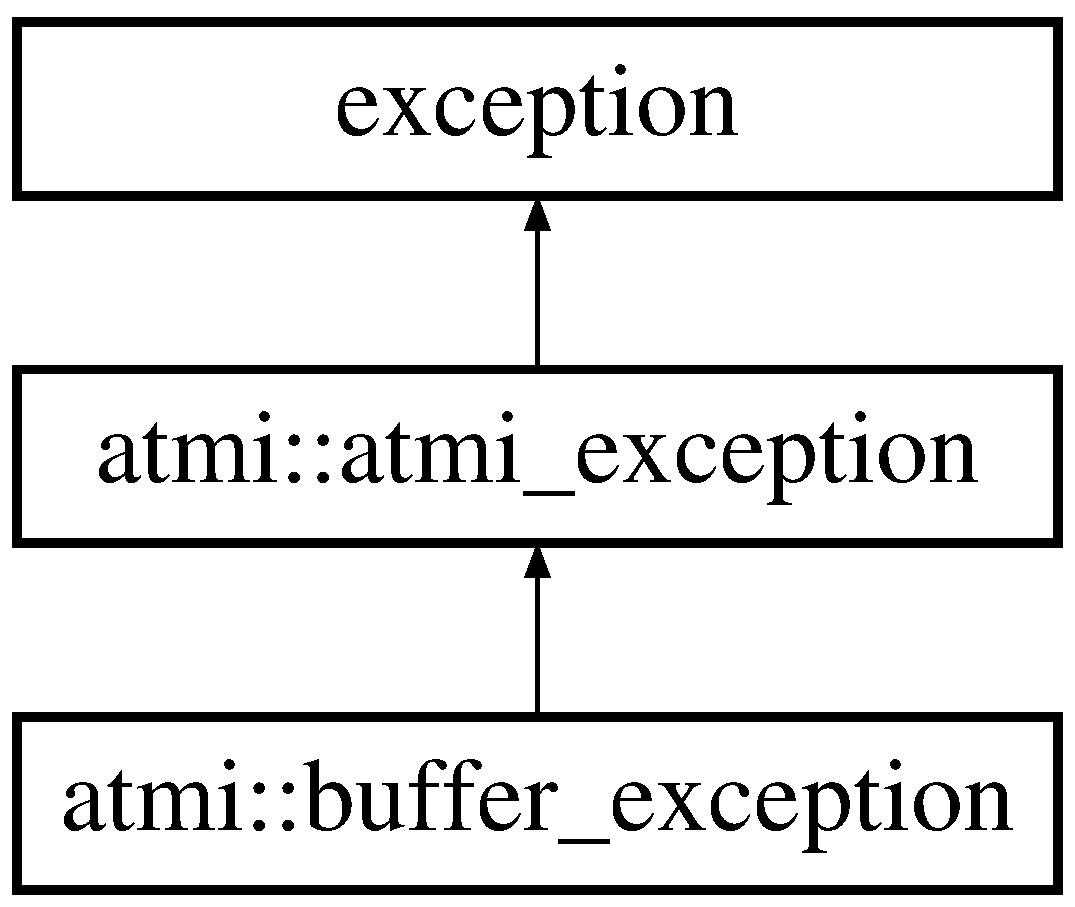
\includegraphics[height=3.000000cm]{classatmi_1_1buffer__exception}
\end{center}
\end{figure}
\subsection*{Public Member Functions}
\begin{DoxyCompactItemize}
\item 
{\footnotesize template$<$typename... Args$>$ }\\\hyperlink{classatmi_1_1buffer__exception_aff48a3528d8a2d575a194233f454bd40}{buffer\+\_\+exception} (int err, const char $\ast$msg, const Args \&...args)
\item 
\hyperlink{classatmi_1_1buffer__exception_a25ef1cb87d75bfca1577f298466e77a0}{buffer\+\_\+exception} ()
\item 
int \hyperlink{classatmi_1_1buffer__exception_a8d9475dbaa7d9864b906dc6ea9818351}{error} () const 
\item 
const char $\ast$ \hyperlink{classatmi_1_1buffer__exception_a6881332c2a607fb71b987eaf811723b7}{error\+\_\+message} () const 
\end{DoxyCompactItemize}
\subsection*{Additional Inherited Members}


\subsection{Detailed Description}
F\+M\+L buffer related exceptions. 

\subsection{Constructor \& Destructor Documentation}
\hypertarget{classatmi_1_1buffer__exception_aff48a3528d8a2d575a194233f454bd40}{\index{atmi\+::buffer\+\_\+exception@{atmi\+::buffer\+\_\+exception}!buffer\+\_\+exception@{buffer\+\_\+exception}}
\index{buffer\+\_\+exception@{buffer\+\_\+exception}!atmi\+::buffer\+\_\+exception@{atmi\+::buffer\+\_\+exception}}
\subsubsection[{buffer\+\_\+exception}]{\setlength{\rightskip}{0pt plus 5cm}template$<$typename... Args$>$ atmi\+::buffer\+\_\+exception\+::buffer\+\_\+exception (
\begin{DoxyParamCaption}
\item[{int}]{err, }
\item[{const char $\ast$}]{msg, }
\item[{const Args \&...}]{args}
\end{DoxyParamCaption}
)\hspace{0.3cm}{\ttfamily [inline]}}}\label{classatmi_1_1buffer__exception_aff48a3528d8a2d575a194233f454bd40}
new buffer exception.


\begin{DoxyParams}{Parameters}
{\em err} & Ferror32 value \\
\hline
{\em msg} & error message \\
\hline
{\em args} & error message parameters (variadic). \\
\hline
\end{DoxyParams}
\hypertarget{classatmi_1_1buffer__exception_a25ef1cb87d75bfca1577f298466e77a0}{\index{atmi\+::buffer\+\_\+exception@{atmi\+::buffer\+\_\+exception}!buffer\+\_\+exception@{buffer\+\_\+exception}}
\index{buffer\+\_\+exception@{buffer\+\_\+exception}!atmi\+::buffer\+\_\+exception@{atmi\+::buffer\+\_\+exception}}
\subsubsection[{buffer\+\_\+exception}]{\setlength{\rightskip}{0pt plus 5cm}atmi\+::buffer\+\_\+exception\+::buffer\+\_\+exception (
\begin{DoxyParamCaption}
{}
\end{DoxyParamCaption}
)}}\label{classatmi_1_1buffer__exception_a25ef1cb87d75bfca1577f298466e77a0}
default constructor.

set error message to strerror. 

\subsection{Member Function Documentation}
\hypertarget{classatmi_1_1buffer__exception_a8d9475dbaa7d9864b906dc6ea9818351}{\index{atmi\+::buffer\+\_\+exception@{atmi\+::buffer\+\_\+exception}!error@{error}}
\index{error@{error}!atmi\+::buffer\+\_\+exception@{atmi\+::buffer\+\_\+exception}}
\subsubsection[{error}]{\setlength{\rightskip}{0pt plus 5cm}int atmi\+::buffer\+\_\+exception\+::error (
\begin{DoxyParamCaption}
{}
\end{DoxyParamCaption}
) const}}\label{classatmi_1_1buffer__exception_a8d9475dbaa7d9864b906dc6ea9818351}
\begin{DoxyReturn}{Returns}
tuxedo F\+M\+L error number 
\end{DoxyReturn}
\hypertarget{classatmi_1_1buffer__exception_a6881332c2a607fb71b987eaf811723b7}{\index{atmi\+::buffer\+\_\+exception@{atmi\+::buffer\+\_\+exception}!error\+\_\+message@{error\+\_\+message}}
\index{error\+\_\+message@{error\+\_\+message}!atmi\+::buffer\+\_\+exception@{atmi\+::buffer\+\_\+exception}}
\subsubsection[{error\+\_\+message}]{\setlength{\rightskip}{0pt plus 5cm}const char $\ast$ atmi\+::buffer\+\_\+exception\+::error\+\_\+message (
\begin{DoxyParamCaption}
{}
\end{DoxyParamCaption}
) const}}\label{classatmi_1_1buffer__exception_a6881332c2a607fb71b987eaf811723b7}
\begin{DoxyReturn}{Returns}
tuxedo F\+M\+L error message string 
\end{DoxyReturn}


The documentation for this class was generated from the following files\+:\begin{DoxyCompactItemize}
\item 
include/atmi/exceptions.\+hpp\item 
src/exceptions.\+cpp\end{DoxyCompactItemize}

\hypertarget{classatmi_1_1call__info}{\section{atmi\+:\+:call\+\_\+info Class Reference}
\label{classatmi_1_1call__info}\index{atmi\+::call\+\_\+info@{atmi\+::call\+\_\+info}}
}
\subsection*{Public Member Functions}
\begin{DoxyCompactItemize}
\item 
const std\+::string \hyperlink{classatmi_1_1call__info_a6ebd3fff62da55b8026f761d4f4dd9c3}{ecid} ()
\item 
void \hyperlink{classatmi_1_1call__info_a737b724e370e1079aecb4ae89314fd13}{set\+\_\+ecid} (const char $\ast$value)
\item 
void \hyperlink{classatmi_1_1call__info_a2c32068c9b16a9f8702f892c9cd50ebd}{print} () const 
\item 
\hyperlink{classatmi_1_1call__info}{call\+\_\+info} \& \hyperlink{classatmi_1_1call__info_aadf1ac5874546447738af60a05d11ad1}{operator=} (\hyperlink{classatmi_1_1call__info}{call\+\_\+info} \&callinfo)
\item 
\hyperlink{classatmi_1_1call__info_adbfaf3240bfd093674ff7d56705fb13f}{operator F\+B\+F\+R32 $\ast$} ()
\item 
\hyperlink{classatmi_1_1call__info_a536f61bc22398ff5422f90679fde8e70}{call\+\_\+info} ()
\end{DoxyCompactItemize}
\subsection*{Friends}
\begin{DoxyCompactItemize}
\item 
void \hyperlink{classatmi_1_1call__info_af62be22be84d07b2d914321ba7f99d41}{buffer\+::get\+\_\+call\+\_\+info} (\hyperlink{classatmi_1_1call__info}{call\+\_\+info} \&callinfo)
\end{DoxyCompactItemize}


\subsection{Constructor \& Destructor Documentation}
\hypertarget{classatmi_1_1call__info_a536f61bc22398ff5422f90679fde8e70}{\index{atmi\+::call\+\_\+info@{atmi\+::call\+\_\+info}!call\+\_\+info@{call\+\_\+info}}
\index{call\+\_\+info@{call\+\_\+info}!atmi\+::call\+\_\+info@{atmi\+::call\+\_\+info}}
\subsubsection[{call\+\_\+info}]{\setlength{\rightskip}{0pt plus 5cm}atmi\+::call\+\_\+info\+::call\+\_\+info (
\begin{DoxyParamCaption}
{}
\end{DoxyParamCaption}
)}}\label{classatmi_1_1call__info_a536f61bc22398ff5422f90679fde8e70}
create a F\+B\+F\+R32 buffer to hold call infos 

\subsection{Member Function Documentation}
\hypertarget{classatmi_1_1call__info_a6ebd3fff62da55b8026f761d4f4dd9c3}{\index{atmi\+::call\+\_\+info@{atmi\+::call\+\_\+info}!ecid@{ecid}}
\index{ecid@{ecid}!atmi\+::call\+\_\+info@{atmi\+::call\+\_\+info}}
\subsubsection[{ecid}]{\setlength{\rightskip}{0pt plus 5cm}const std\+::string atmi\+::call\+\_\+info\+::ecid (
\begin{DoxyParamCaption}
{}
\end{DoxyParamCaption}
)}}\label{classatmi_1_1call__info_a6ebd3fff62da55b8026f761d4f4dd9c3}
\begin{DoxyReturn}{Returns}
current E\+C\+I\+D value 
\end{DoxyReturn}
\hypertarget{classatmi_1_1call__info_adbfaf3240bfd093674ff7d56705fb13f}{\index{atmi\+::call\+\_\+info@{atmi\+::call\+\_\+info}!operator F\+B\+F\+R32 $\ast$@{operator F\+B\+F\+R32 $\ast$}}
\index{operator F\+B\+F\+R32 $\ast$@{operator F\+B\+F\+R32 $\ast$}!atmi\+::call\+\_\+info@{atmi\+::call\+\_\+info}}
\subsubsection[{operator F\+B\+F\+R32 $\ast$}]{\setlength{\rightskip}{0pt plus 5cm}atmi\+::call\+\_\+info\+::operator F\+B\+F\+R32 $\ast$ (
\begin{DoxyParamCaption}
{}
\end{DoxyParamCaption}
)}}\label{classatmi_1_1call__info_adbfaf3240bfd093674ff7d56705fb13f}
\begin{DoxyReturn}{Returns}
a F\+B\+F\+R32 $\ast$ buffer that contains the call infos 
\end{DoxyReturn}
\hypertarget{classatmi_1_1call__info_aadf1ac5874546447738af60a05d11ad1}{\index{atmi\+::call\+\_\+info@{atmi\+::call\+\_\+info}!operator=@{operator=}}
\index{operator=@{operator=}!atmi\+::call\+\_\+info@{atmi\+::call\+\_\+info}}
\subsubsection[{operator=}]{\setlength{\rightskip}{0pt plus 5cm}{\bf call\+\_\+info} \& atmi\+::call\+\_\+info\+::operator= (
\begin{DoxyParamCaption}
\item[{{\bf atmi\+::call\+\_\+info} \&}]{callinfo}
\end{DoxyParamCaption}
)}}\label{classatmi_1_1call__info_aadf1ac5874546447738af60a05d11ad1}
copy (Fcopy32) a call info buffer


\begin{DoxyParams}{Parameters}
{\em callinfo} & call info content to copy. \\
\hline
\end{DoxyParams}
\begin{DoxyReturn}{Returns}
\hyperlink{classatmi_1_1call__info}{call\+\_\+info} reference 
\end{DoxyReturn}
\hypertarget{classatmi_1_1call__info_a2c32068c9b16a9f8702f892c9cd50ebd}{\index{atmi\+::call\+\_\+info@{atmi\+::call\+\_\+info}!print@{print}}
\index{print@{print}!atmi\+::call\+\_\+info@{atmi\+::call\+\_\+info}}
\subsubsection[{print}]{\setlength{\rightskip}{0pt plus 5cm}void atmi\+::call\+\_\+info\+::print (
\begin{DoxyParamCaption}
{}
\end{DoxyParamCaption}
) const}}\label{classatmi_1_1call__info_a2c32068c9b16a9f8702f892c9cd50ebd}
print call infos \hypertarget{classatmi_1_1call__info_a737b724e370e1079aecb4ae89314fd13}{\index{atmi\+::call\+\_\+info@{atmi\+::call\+\_\+info}!set\+\_\+ecid@{set\+\_\+ecid}}
\index{set\+\_\+ecid@{set\+\_\+ecid}!atmi\+::call\+\_\+info@{atmi\+::call\+\_\+info}}
\subsubsection[{set\+\_\+ecid}]{\setlength{\rightskip}{0pt plus 5cm}void atmi\+::call\+\_\+info\+::set\+\_\+ecid (
\begin{DoxyParamCaption}
\item[{const char $\ast$}]{value}
\end{DoxyParamCaption}
)}}\label{classatmi_1_1call__info_a737b724e370e1079aecb4ae89314fd13}
update/set E\+C\+I\+D.


\begin{DoxyParams}{Parameters}
{\em value} & ecid \\
\hline
\end{DoxyParams}
\begin{DoxySeeAlso}{See also}
atmi\+::buffer\+::set\+\_\+cal\+\_\+info 
\end{DoxySeeAlso}


\subsection{Friends And Related Function Documentation}
\hypertarget{classatmi_1_1call__info_af62be22be84d07b2d914321ba7f99d41}{\index{atmi\+::call\+\_\+info@{atmi\+::call\+\_\+info}!buffer\+::get\+\_\+call\+\_\+info@{buffer\+::get\+\_\+call\+\_\+info}}
\index{buffer\+::get\+\_\+call\+\_\+info@{buffer\+::get\+\_\+call\+\_\+info}!atmi\+::call\+\_\+info@{atmi\+::call\+\_\+info}}
\subsubsection[{buffer\+::get\+\_\+call\+\_\+info}]{\setlength{\rightskip}{0pt plus 5cm}void {\bf buffer\+::get\+\_\+call\+\_\+info} (
\begin{DoxyParamCaption}
\item[{{\bf call\+\_\+info} \&}]{callinfo}
\end{DoxyParamCaption}
)\hspace{0.3cm}{\ttfamily [friend]}}}\label{classatmi_1_1call__info_af62be22be84d07b2d914321ba7f99d41}
give private access to this trusted friend \+:-\/)


\begin{DoxyParams}{Parameters}
{\em callinfo} & Tuxedo call metadata \\
\hline
\end{DoxyParams}


The documentation for this class was generated from the following files\+:\begin{DoxyCompactItemize}
\item 
include/atmi/call\+\_\+info.\+hpp\item 
src/call\+\_\+info.\+cpp\end{DoxyCompactItemize}

\hypertarget{classatmi_1_1diagnostic__exception}{}\section{atmi\+:\+:diagnostic\+\_\+exception Class Reference}
\label{classatmi_1_1diagnostic__exception}\index{atmi\+::diagnostic\+\_\+exception@{atmi\+::diagnostic\+\_\+exception}}


{\ttfamily \#include $<$exceptions.\+hpp$>$}

Inheritance diagram for atmi\+:\+:diagnostic\+\_\+exception\+:\begin{figure}[H]
\begin{center}
\leavevmode
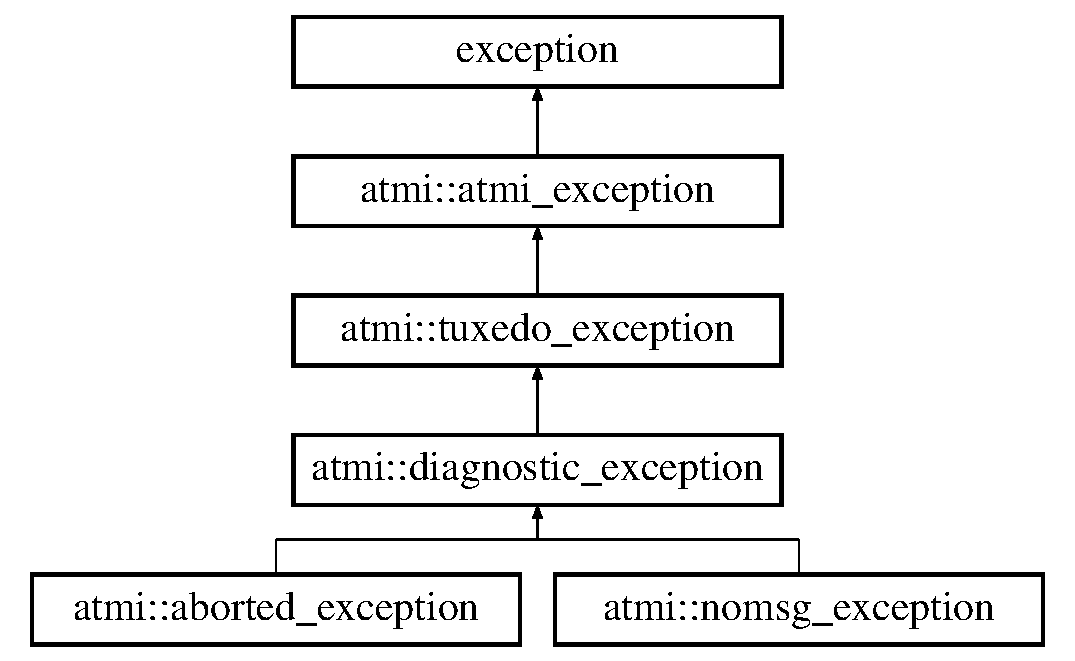
\includegraphics[height=5.000000cm]{classatmi_1_1diagnostic__exception}
\end{center}
\end{figure}
\subsection*{Public Member Functions}
\begin{DoxyCompactItemize}
\item 
{\footnotesize template$<$typename... Args$>$ }\\\hyperlink{classatmi_1_1diagnostic__exception_acf086c2efbe447d733a02988e56be370}{diagnostic\+\_\+exception} (int err, long diagno, const char $\ast$msg, const Args \&...args)
\item 
long \hyperlink{classatmi_1_1diagnostic__exception_a5602718873c6e8122af75d5adf9d375b}{diagnostic} () const 
\item 
const char $\ast$ \hyperlink{classatmi_1_1diagnostic__exception_a60931362229b54fc6847a3efa5e83ffd}{diagnostic\+\_\+message} () const 
\end{DoxyCompactItemize}
\subsection*{Additional Inherited Members}


\subsection{Detailed Description}
/Q related exceptions 

\subsection{Constructor \& Destructor Documentation}
\index{atmi\+::diagnostic\+\_\+exception@{atmi\+::diagnostic\+\_\+exception}!diagnostic\+\_\+exception@{diagnostic\+\_\+exception}}
\index{diagnostic\+\_\+exception@{diagnostic\+\_\+exception}!atmi\+::diagnostic\+\_\+exception@{atmi\+::diagnostic\+\_\+exception}}
\subsubsection[{\texorpdfstring{diagnostic\+\_\+exception(int err, long diagno, const char $\ast$msg, const Args \&...\+args)}{diagnostic\_exception(int err, long diagno, const char *msg, const Args \&...args)}}]{\setlength{\rightskip}{0pt plus 5cm}template$<$typename... Args$>$ atmi\+::diagnostic\+\_\+exception\+::diagnostic\+\_\+exception (
\begin{DoxyParamCaption}
\item[{int}]{err, }
\item[{long}]{diagno, }
\item[{const char $\ast$}]{msg, }
\item[{const Args \&...}]{args}
\end{DoxyParamCaption}
)\hspace{0.3cm}{\ttfamily [inline]}}\hypertarget{classatmi_1_1diagnostic__exception_acf086c2efbe447d733a02988e56be370}{}\label{classatmi_1_1diagnostic__exception_acf086c2efbe447d733a02988e56be370}
Constructs a Queue exeption


\begin{DoxyParams}{Parameters}
{\em err} & value of tperr \\
\hline
{\em diagno} & value of ctl.\+diagnostic \\
\hline
{\em msg} & error message format. \\
\hline
{\em args} & error message parameters (variadic). \\
\hline
\end{DoxyParams}


\subsection{Member Function Documentation}
\index{atmi\+::diagnostic\+\_\+exception@{atmi\+::diagnostic\+\_\+exception}!diagnostic@{diagnostic}}
\index{diagnostic@{diagnostic}!atmi\+::diagnostic\+\_\+exception@{atmi\+::diagnostic\+\_\+exception}}
\subsubsection[{\texorpdfstring{diagnostic() const }{diagnostic() const }}]{\setlength{\rightskip}{0pt plus 5cm}long atmi\+::diagnostic\+\_\+exception\+::diagnostic (
\begin{DoxyParamCaption}
{}
\end{DoxyParamCaption}
) const\hspace{0.3cm}{\ttfamily [inline]}}\hypertarget{classatmi_1_1diagnostic__exception_a5602718873c6e8122af75d5adf9d375b}{}\label{classatmi_1_1diagnostic__exception_a5602718873c6e8122af75d5adf9d375b}
\begin{DoxyReturn}{Returns}
tuxedo diagnostic error number 
\end{DoxyReturn}
\index{atmi\+::diagnostic\+\_\+exception@{atmi\+::diagnostic\+\_\+exception}!diagnostic\+\_\+message@{diagnostic\+\_\+message}}
\index{diagnostic\+\_\+message@{diagnostic\+\_\+message}!atmi\+::diagnostic\+\_\+exception@{atmi\+::diagnostic\+\_\+exception}}
\subsubsection[{\texorpdfstring{diagnostic\+\_\+message() const }{diagnostic\_message() const }}]{\setlength{\rightskip}{0pt plus 5cm}const char $\ast$ atmi\+::diagnostic\+\_\+exception\+::diagnostic\+\_\+message (
\begin{DoxyParamCaption}
{}
\end{DoxyParamCaption}
) const}\hypertarget{classatmi_1_1diagnostic__exception_a60931362229b54fc6847a3efa5e83ffd}{}\label{classatmi_1_1diagnostic__exception_a60931362229b54fc6847a3efa5e83ffd}
\begin{DoxyReturn}{Returns}
diagnostic error message string 
\end{DoxyReturn}


The documentation for this class was generated from the following files\+:\begin{DoxyCompactItemize}
\item 
include/atmi/exceptions.\+hpp\item 
src/exceptions.\+cpp\end{DoxyCompactItemize}

\hypertarget{classatmi_1_1event}{}\section{atmi\+:\+:event Class Reference}
\label{classatmi_1_1event}\index{atmi\+::event@{atmi\+::event}}


{\ttfamily \#include $<$event.\+hpp$>$}

Inheritance diagram for atmi\+:\+:event\+:\begin{figure}[H]
\begin{center}
\leavevmode
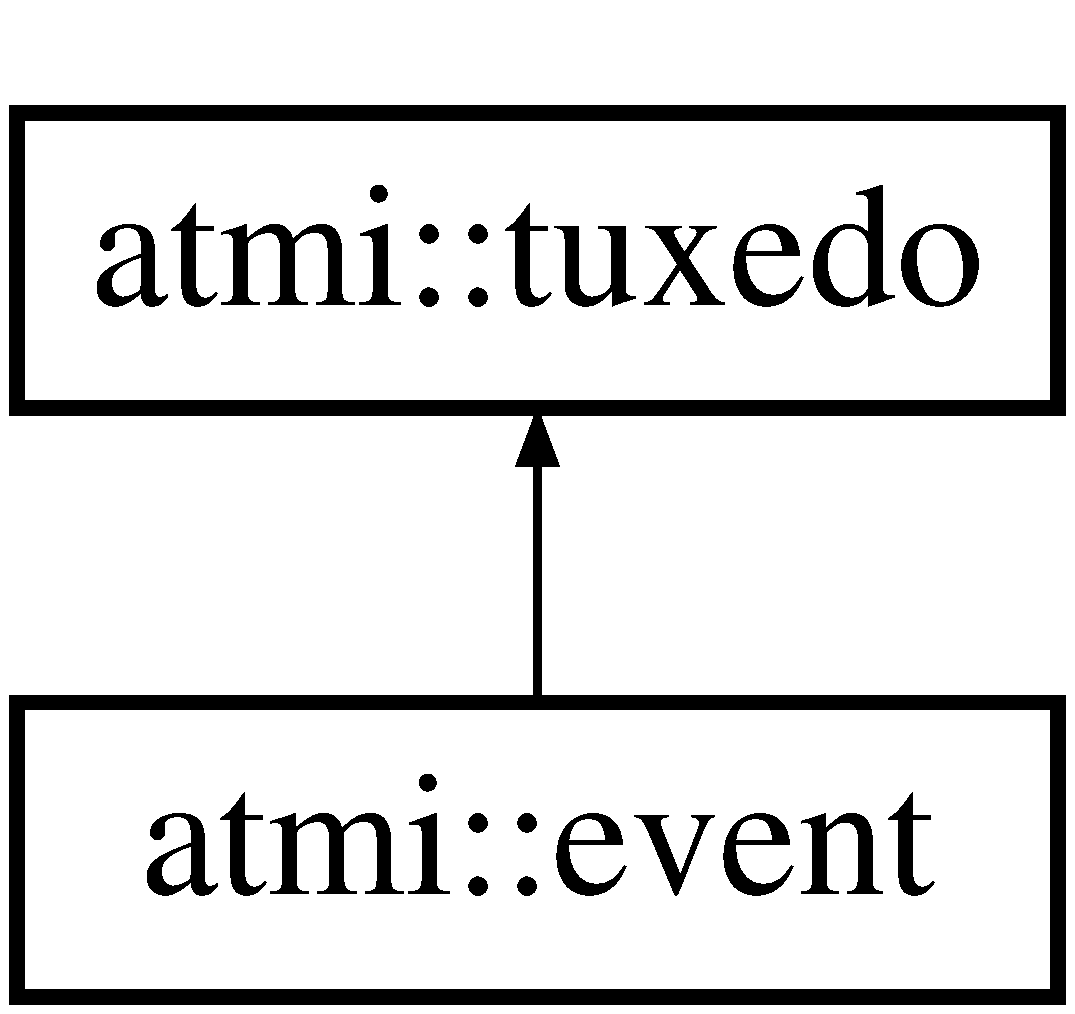
\includegraphics[height=2.000000cm]{classatmi_1_1event}
\end{center}
\end{figure}
\subsection*{Public Member Functions}
\begin{DoxyCompactItemize}
\item 
\hyperlink{classatmi_1_1event_a64e8905f6b027d052074cb801567b1b3}{event} (const char $\ast$evtname=N\+U\+LL)
\item 
long \hyperlink{classatmi_1_1event_a0b1f1faae17aa923ce5a4a0d45cfcd07}{post} (const char $\ast$data=N\+U\+LL, long len=0)  throw ( tuxedo\+\_\+exception )
\end{DoxyCompactItemize}
\subsection*{Additional Inherited Members}


\subsection{Detailed Description}
Use this class to post an event and any accompanying data. The event is named by eventname and data, if not N\+U\+LL, points to the data. The posted event and its data are dispatched by the Oracle tuxedo A\+T\+MI event\+Broker to all subscribers whose subscriptions successfully evaluate against eventname and whose optional filter rules successfully evaluate against data.

eventname is a N\+U\+L\+L-\/terminated string of at most 31 characters. eventname’s first character cannot be a dot (“.\+”) as this character is reserved as the starting character for all events defined by the Oracle tuxedo A\+T\+MI system itself.

If data is non-\/\+N\+U\+LL, it must point to a buffer previously allocated by tpalloc() and len should specify the amount of data in the buffer that should be posted with the event. Note that if data points to a buffer of a type that does not require a length to be specified (for example, an F\+ML fielded buffer), then len is ignored. If data is N\+U\+LL, len is ignored and the event is posted with no data.

When event is used within a transaction, the transaction boundary can be extended to include those servers and/or stable-\/storage message queues notified by the event\+Broker. When a transactional posting is made, some of the recipients of the event posting are notified on behalf of the poster’s transaction (for example, servers and queues), while some are not (for example, clients).

If the poster is within a transaction and the T\+P\+N\+O\+T\+R\+AN flag is not set, the posted event goes to the event\+Broker in transaction mode such that it dispatches the event as part of the poster’s transaction. The broker dispatches transactional event notifications only to those service routine and stable-\/storage queue subscriptions that used the T\+P\+E\+V\+T\+R\+AN bit setting in the ctlflags parameter passed to subscribe(). Client notifications, and those service routine and stable-\/storage queue subscriptions that did not use the T\+P\+E\+V\+T\+R\+AN bit setting in the ctlflags parameter passed to subscribe(), are also dispatched by the event\+Broker but not as part of the posting process’s transaction.

If the poster is outside a transaction, \hyperlink{classatmi_1_1event_a0b1f1faae17aa923ce5a4a0d45cfcd07}{post()} is a one-\/way post with no acknowledgement when the service associated with the event fails. This occurs even when T\+P\+E\+V\+T\+R\+AN is set for that event (using the ctlflags parameter passed to subscribe()). If the poster is in a transaction, then \hyperlink{classatmi_1_1event_a0b1f1faae17aa923ce5a4a0d45cfcd07}{post()} returns T\+P\+E\+S\+V\+C\+F\+A\+IL when the associated service fails in the event. 

\subsection{Constructor \& Destructor Documentation}
\index{atmi\+::event@{atmi\+::event}!event@{event}}
\index{event@{event}!atmi\+::event@{atmi\+::event}}
\subsubsection[{\texorpdfstring{event(const char $\ast$evtname=\+N\+U\+L\+L)}{event(const char *evtname=NULL)}}]{\setlength{\rightskip}{0pt plus 5cm}atmi\+::event\+::event (
\begin{DoxyParamCaption}
\item[{const char $\ast$}]{evtname = {\ttfamily NULL}}
\end{DoxyParamCaption}
)\hspace{0.3cm}{\ttfamily [explicit]}}\hypertarget{classatmi_1_1event_a64e8905f6b027d052074cb801567b1b3}{}\label{classatmi_1_1event_a64e8905f6b027d052074cb801567b1b3}
Use this class to post an event and any accompanying data. The event is named by eventname and data, if not N\+U\+LL, points to the data. The posted event and its data are dispatched by the Oracle tuxedo A\+T\+MI event\+Broker to all subscribers whose subscriptions successfully evaluate against eventname and whose optional filter rules successfully evaluate against data.


\begin{DoxyParams}{Parameters}
{\em evtname} & is a N\+U\+L\+L-\/terminated string of at most 31 characters. eventname’s first character cannot be a dot (“.\+”) as this character is reserved by the Oracle tuxedo A\+T\+MI system itself. \\
\hline
\end{DoxyParams}


\subsection{Member Function Documentation}
\index{atmi\+::event@{atmi\+::event}!post@{post}}
\index{post@{post}!atmi\+::event@{atmi\+::event}}
\subsubsection[{\texorpdfstring{post(const char $\ast$data=\+N\+U\+L\+L, long len=0)}{post(const char *data=NULL, long len=0)}}]{\setlength{\rightskip}{0pt plus 5cm}long atmi\+::event\+::post (
\begin{DoxyParamCaption}
\item[{const char $\ast$}]{data = {\ttfamily NULL}, }
\item[{long}]{len = {\ttfamily 0}}
\end{DoxyParamCaption}
) throw  {\bf tuxedo\+\_\+exception}) }\hypertarget{classatmi_1_1event_a0b1f1faae17aa923ce5a4a0d45cfcd07}{}\label{classatmi_1_1event_a0b1f1faae17aa923ce5a4a0d45cfcd07}
The caller uses \hyperlink{classatmi_1_1event_a0b1f1faae17aa923ce5a4a0d45cfcd07}{post()} to post an event and any accompanying data. The event is named by eventname and data, if not N\+U\+LL, points to the data. The posted event and its data are dispatched by the Oracle tuxedo A\+T\+MI event\+Broker to all subscribers whose subscriptions successfully evaluate against eventname and whose optional filter rules successfully evaluate against data.


\begin{DoxyParams}{Parameters}
{\em data} & it must point to a buffer previously allocated by \hyperlink{classatmi_1_1tuxedo_a44e77e3e6216a8c3fb8be33d5d8fed93}{allocate()} \\
\hline
{\em len} & len should specify the amount of data in the buffer that should be posted with the event.\\
\hline
\end{DoxyParams}
\begin{DoxyReturn}{Returns}
number of notifications number of event notifications dispatched by the event\+Broker on behalf of eventname. 
\end{DoxyReturn}


The documentation for this class was generated from the following files\+:\begin{DoxyCompactItemize}
\item 
include/atmi/event.\+hpp\item 
src/event.\+cpp\end{DoxyCompactItemize}

\hypertarget{classatmi_1_1field}{\section{atmi\+:\+:field Class Reference}
\label{classatmi_1_1field}\index{atmi\+::field@{atmi\+::field}}
}


{\ttfamily \#include $<$fields.\+hpp$>$}

Inheritance diagram for atmi\+:\+:field\+:\begin{figure}[H]
\begin{center}
\leavevmode
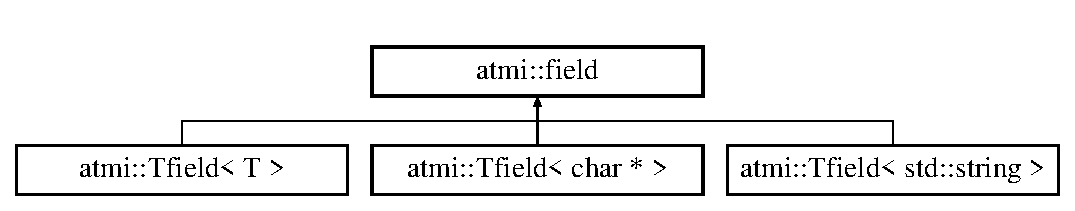
\includegraphics[height=2.000000cm]{classatmi_1_1field}
\end{center}
\end{figure}
\subsection*{Public Member Functions}
\begin{DoxyCompactItemize}
\item 
\hyperlink{classatmi_1_1field_ad704c8d557c86b84b2d37bdf2cbdc36c}{field} ()
\item 
virtual \hyperlink{classatmi_1_1field_a6f91cba3fca0a77fb7ad229187d689b9}{$\sim$field} ()
\item 
int \hyperlink{classatmi_1_1field_a717c701f07a784f471abb44d7bc95048}{type} ()
\item 
const char $\ast$ \hyperlink{classatmi_1_1field_a7d6260dd6f7c3c44de29190c2dfd546e}{tname} ()
\item 
F\+L\+D\+I\+D32 \hyperlink{classatmi_1_1field_a89ff294c8276c6a882f510a8f95ac372}{id} () const 
\item 
virtual void \hyperlink{classatmi_1_1field_a1d95c3b0f4ae491037ef51b8586a0083}{set\+\_\+id} (F\+L\+D\+I\+D32 \hyperlink{classatmi_1_1field_a89ff294c8276c6a882f510a8f95ac372}{id})
\item 
int \hyperlink{classatmi_1_1field_aa71d28f3df8490e9ed016607f857fae1}{number} ()
\item 
const char $\ast$ \hyperlink{classatmi_1_1field_a0fbc5a958a0af8286e339b088ee69bc8}{name} ()
\item 
F\+L\+D\+O\+C\+C32 \hyperlink{classatmi_1_1field_a161b9b7037c49fbcf86518fcb35e779c}{occurence} ()
\item 
int \hyperlink{classatmi_1_1field_a6d8db988f58f3779b0ef528a11b3466f}{error} ()
\item 
virtual F\+L\+D\+L\+E\+N32 \hyperlink{classatmi_1_1field_a296771293135085d91aa9aefd108d44d}{length} ()=0
\item 
virtual long \hyperlink{classatmi_1_1field_aef2940ef13d554b2a0090ea4052529d8}{needed} ()
\item 
const char $\ast$ \hyperlink{classatmi_1_1field_a396b41ad5ae2b1df362e446c5f090640}{what} ()
\item 
virtual \hyperlink{classatmi_1_1field}{field} \& \hyperlink{classatmi_1_1field_addd031ecbcf2026116cf6e03534ac862}{operator=} (const std\+::string \&value)
\end{DoxyCompactItemize}
\subsection*{Protected Member Functions}
\begin{DoxyCompactItemize}
\item 
virtual void \hyperlink{classatmi_1_1field_a83412cd9df383c342b5feb195090c9d9}{set\+\_\+field\+\_\+occurence} (F\+L\+D\+O\+C\+C32 occ)
\item 
virtual void \hyperlink{classatmi_1_1field_a9ca5e61e3e1068770098d20ad1332f24}{setup} (F\+L\+D\+I\+D32 field\+\_\+id)
\item 
virtual int \hyperlink{classatmi_1_1field_aae2d3df756e816b5db8f729039a59a51}{get} (\hyperlink{classatmi_1_1buffer}{buffer} \&b)=0
\item 
virtual int \hyperlink{classatmi_1_1field_a56ce53fabe290b94463f87936515ec46}{get} (\hyperlink{classatmi_1_1buffer}{buffer} \&b, F\+L\+D\+O\+C\+C32 occ)=0
\item 
virtual int \hyperlink{classatmi_1_1field_a5441bc87ba4bc3e9eb37c6db6a29688f}{add} (\hyperlink{classatmi_1_1buffer}{buffer} \&b)=0
\item 
virtual int \hyperlink{classatmi_1_1field_a41bb209965d627d2e67c839bece5372c}{set} (\hyperlink{classatmi_1_1buffer}{buffer} \&b)=0
\item 
virtual int \hyperlink{classatmi_1_1field_a783484fe641f66f5773f9eed7fd4be39}{remove} (\hyperlink{classatmi_1_1buffer}{buffer} \&b)
\end{DoxyCompactItemize}
\subsection*{Friends}
\begin{DoxyCompactItemize}
\item 
\hypertarget{classatmi_1_1field_afecbc2840248040e50fecb7164f912a9}{class {\bfseries buffer}}\label{classatmi_1_1field_afecbc2840248040e50fecb7164f912a9}

\end{DoxyCompactItemize}


\subsection{Detailed Description}
When a new instance is created, occurence is set to 0 making it possible to set values withour a prior call to add. 

\subsection{Constructor \& Destructor Documentation}
\hypertarget{classatmi_1_1field_ad704c8d557c86b84b2d37bdf2cbdc36c}{\index{atmi\+::field@{atmi\+::field}!field@{field}}
\index{field@{field}!atmi\+::field@{atmi\+::field}}
\subsubsection[{field}]{\setlength{\rightskip}{0pt plus 5cm}atmi\+::field\+::field (
\begin{DoxyParamCaption}
{}
\end{DoxyParamCaption}
)}}\label{classatmi_1_1field_ad704c8d557c86b84b2d37bdf2cbdc36c}
default constructor

default occurence value is 0. \hypertarget{classatmi_1_1field_a6f91cba3fca0a77fb7ad229187d689b9}{\index{atmi\+::field@{atmi\+::field}!````~field@{$\sim$field}}
\index{````~field@{$\sim$field}!atmi\+::field@{atmi\+::field}}
\subsubsection[{$\sim$field}]{\setlength{\rightskip}{0pt plus 5cm}virtual atmi\+::field\+::$\sim$field (
\begin{DoxyParamCaption}
{}
\end{DoxyParamCaption}
)\hspace{0.3cm}{\ttfamily [inline]}, {\ttfamily [virtual]}}}\label{classatmi_1_1field_a6f91cba3fca0a77fb7ad229187d689b9}
Default destructor 

\subsection{Member Function Documentation}
\hypertarget{classatmi_1_1field_a5441bc87ba4bc3e9eb37c6db6a29688f}{\index{atmi\+::field@{atmi\+::field}!add@{add}}
\index{add@{add}!atmi\+::field@{atmi\+::field}}
\subsubsection[{add}]{\setlength{\rightskip}{0pt plus 5cm}virtual int atmi\+::field\+::add (
\begin{DoxyParamCaption}
\item[{{\bf buffer} \&}]{b}
\end{DoxyParamCaption}
)\hspace{0.3cm}{\ttfamily [protected]}, {\ttfamily [pure virtual]}}}\label{classatmi_1_1field_a5441bc87ba4bc3e9eb37c6db6a29688f}
add the fiels into the buffer

When successfull the value of occurence is se


\begin{DoxyParams}{Parameters}
{\em b} & buffer in which to add the field. \\
\hline
\end{DoxyParams}
\begin{DoxySeeAlso}{See also}
\hyperlink{classatmi_1_1field_a161b9b7037c49fbcf86518fcb35e779c}{occurence} 
\end{DoxySeeAlso}


Implemented in \hyperlink{classatmi_1_1_tfield_3_01std_1_1string_01_4_af17fc3c22ce857f9d96f96d6c175b6d5}{atmi\+::\+Tfield$<$ std\+::string $>$}, \hyperlink{classatmi_1_1_tfield_a4962b3aa080aba4ecffc7f3fa98be2da}{atmi\+::\+Tfield$<$ T $>$}, and \hyperlink{classatmi_1_1_tfield_3_01char_01_5_01_4_ae3036c038b361aee2fc357c1c7d1304a}{atmi\+::\+Tfield$<$ char $\ast$ $>$}.

\hypertarget{classatmi_1_1field_a6d8db988f58f3779b0ef528a11b3466f}{\index{atmi\+::field@{atmi\+::field}!error@{error}}
\index{error@{error}!atmi\+::field@{atmi\+::field}}
\subsubsection[{error}]{\setlength{\rightskip}{0pt plus 5cm}int atmi\+::field\+::error (
\begin{DoxyParamCaption}
{}
\end{DoxyParamCaption}
)}}\label{classatmi_1_1field_a6d8db988f58f3779b0ef528a11b3466f}
\begin{DoxyReturn}{Returns}
the last Ferror32 value that was returned by the F\+M\+L library 
\end{DoxyReturn}
\hypertarget{classatmi_1_1field_aae2d3df756e816b5db8f729039a59a51}{\index{atmi\+::field@{atmi\+::field}!get@{get}}
\index{get@{get}!atmi\+::field@{atmi\+::field}}
\subsubsection[{get}]{\setlength{\rightskip}{0pt plus 5cm}virtual int atmi\+::field\+::get (
\begin{DoxyParamCaption}
\item[{{\bf buffer} \&}]{b}
\end{DoxyParamCaption}
)\hspace{0.3cm}{\ttfamily [protected]}, {\ttfamily [pure virtual]}}}\label{classatmi_1_1field_aae2d3df756e816b5db8f729039a59a51}
Retrieves the value of the field found into the buffer.


\begin{DoxyParams}{Parameters}
{\em b} & buffer from which to retrieve the field's value \\
\hline
\end{DoxyParams}


Implemented in \hyperlink{classatmi_1_1_tfield_3_01std_1_1string_01_4_afecf8218a3c312df34c36f334c995ac7}{atmi\+::\+Tfield$<$ std\+::string $>$}, \hyperlink{classatmi_1_1_tfield_aa70ce8893913c8f3d968cae72f2cdd11}{atmi\+::\+Tfield$<$ T $>$}, and \hyperlink{classatmi_1_1_tfield_3_01char_01_5_01_4_a5df77c9bee99916f6d14f5beeec54dac}{atmi\+::\+Tfield$<$ char $\ast$ $>$}.

\hypertarget{classatmi_1_1field_a56ce53fabe290b94463f87936515ec46}{\index{atmi\+::field@{atmi\+::field}!get@{get}}
\index{get@{get}!atmi\+::field@{atmi\+::field}}
\subsubsection[{get}]{\setlength{\rightskip}{0pt plus 5cm}virtual int atmi\+::field\+::get (
\begin{DoxyParamCaption}
\item[{{\bf buffer} \&}]{b, }
\item[{F\+L\+D\+O\+C\+C32}]{occ}
\end{DoxyParamCaption}
)\hspace{0.3cm}{\ttfamily [protected]}, {\ttfamily [pure virtual]}}}\label{classatmi_1_1field_a56ce53fabe290b94463f87936515ec46}
Retrieves the value of the field's occurence found into the buffer

Upon success the value of occurence is set to the retrieved occurence.


\begin{DoxyParams}{Parameters}
{\em b} & buffer from which to retrieve the field's value \\
\hline
{\em occ} & occurence to retreive \\
\hline
\end{DoxyParams}
\begin{DoxySeeAlso}{See also}
\hyperlink{classatmi_1_1field_a161b9b7037c49fbcf86518fcb35e779c}{occurence} 
\end{DoxySeeAlso}


Implemented in \hyperlink{classatmi_1_1_tfield_3_01std_1_1string_01_4_a34f9956af4b0b98730595258e6c251e2}{atmi\+::\+Tfield$<$ std\+::string $>$}, \hyperlink{classatmi_1_1_tfield_ae8de2dd360d04fc2465e4169b239c222}{atmi\+::\+Tfield$<$ T $>$}, and \hyperlink{classatmi_1_1_tfield_3_01char_01_5_01_4_afaedd7d5902233652bed642bdceb9db1}{atmi\+::\+Tfield$<$ char $\ast$ $>$}.

\hypertarget{classatmi_1_1field_a89ff294c8276c6a882f510a8f95ac372}{\index{atmi\+::field@{atmi\+::field}!id@{id}}
\index{id@{id}!atmi\+::field@{atmi\+::field}}
\subsubsection[{id}]{\setlength{\rightskip}{0pt plus 5cm}F\+L\+D\+I\+D32 atmi\+::field\+::id (
\begin{DoxyParamCaption}
{}
\end{DoxyParamCaption}
) const}}\label{classatmi_1_1field_a89ff294c8276c6a882f510a8f95ac372}
\begin{DoxyReturn}{Returns}
the field I\+D of the field 
\end{DoxyReturn}
\hypertarget{classatmi_1_1field_a296771293135085d91aa9aefd108d44d}{\index{atmi\+::field@{atmi\+::field}!length@{length}}
\index{length@{length}!atmi\+::field@{atmi\+::field}}
\subsubsection[{length}]{\setlength{\rightskip}{0pt plus 5cm}virtual F\+L\+D\+L\+E\+N32 atmi\+::field\+::length (
\begin{DoxyParamCaption}
{}
\end{DoxyParamCaption}
)\hspace{0.3cm}{\ttfamily [pure virtual]}}}\label{classatmi_1_1field_a296771293135085d91aa9aefd108d44d}
\begin{DoxyReturn}{Returns}
the length of the field's value 
\end{DoxyReturn}


Implemented in \hyperlink{classatmi_1_1_tfield_3_01std_1_1string_01_4_ac4fdf6b5f9d1929b34bddc97274c6c9b}{atmi\+::\+Tfield$<$ std\+::string $>$}, \hyperlink{classatmi_1_1_tfield_a6138c508841c4a837ea8c8e089755278}{atmi\+::\+Tfield$<$ T $>$}, and \hyperlink{classatmi_1_1_tfield_3_01char_01_5_01_4_aa97dec8559724186b62997409f04bf3f}{atmi\+::\+Tfield$<$ char $\ast$ $>$}.

\hypertarget{classatmi_1_1field_a0fbc5a958a0af8286e339b088ee69bc8}{\index{atmi\+::field@{atmi\+::field}!name@{name}}
\index{name@{name}!atmi\+::field@{atmi\+::field}}
\subsubsection[{name}]{\setlength{\rightskip}{0pt plus 5cm}const char $\ast$ atmi\+::field\+::name (
\begin{DoxyParamCaption}
{}
\end{DoxyParamCaption}
)}}\label{classatmi_1_1field_a0fbc5a958a0af8286e339b088ee69bc8}
\begin{DoxyReturn}{Returns}
the name of the field 
\end{DoxyReturn}
\hypertarget{classatmi_1_1field_aef2940ef13d554b2a0090ea4052529d8}{\index{atmi\+::field@{atmi\+::field}!needed@{needed}}
\index{needed@{needed}!atmi\+::field@{atmi\+::field}}
\subsubsection[{needed}]{\setlength{\rightskip}{0pt plus 5cm}long atmi\+::field\+::needed (
\begin{DoxyParamCaption}
{}
\end{DoxyParamCaption}
)\hspace{0.3cm}{\ttfamily [virtual]}}}\label{classatmi_1_1field_aef2940ef13d554b2a0090ea4052529d8}
\begin{DoxyReturn}{Returns}
number bytes needed to store the fields value 
\end{DoxyReturn}
\hypertarget{classatmi_1_1field_aa71d28f3df8490e9ed016607f857fae1}{\index{atmi\+::field@{atmi\+::field}!number@{number}}
\index{number@{number}!atmi\+::field@{atmi\+::field}}
\subsubsection[{number}]{\setlength{\rightskip}{0pt plus 5cm}int atmi\+::field\+::number (
\begin{DoxyParamCaption}
{}
\end{DoxyParamCaption}
)}}\label{classatmi_1_1field_aa71d28f3df8490e9ed016607f857fae1}
Extracts the field number from the field identifier.

\begin{DoxyReturn}{Returns}
field number. 
\end{DoxyReturn}
\hypertarget{classatmi_1_1field_a161b9b7037c49fbcf86518fcb35e779c}{\index{atmi\+::field@{atmi\+::field}!occurence@{occurence}}
\index{occurence@{occurence}!atmi\+::field@{atmi\+::field}}
\subsubsection[{occurence}]{\setlength{\rightskip}{0pt plus 5cm}F\+L\+D\+O\+C\+C32 atmi\+::field\+::occurence (
\begin{DoxyParamCaption}
{}
\end{DoxyParamCaption}
)}}\label{classatmi_1_1field_a161b9b7037c49fbcf86518fcb35e779c}
\begin{DoxyReturn}{Returns}
the fields occurence (as last found in a buffer) 
\end{DoxyReturn}
\hypertarget{classatmi_1_1field_addd031ecbcf2026116cf6e03534ac862}{\index{atmi\+::field@{atmi\+::field}!operator=@{operator=}}
\index{operator=@{operator=}!atmi\+::field@{atmi\+::field}}
\subsubsection[{operator=}]{\setlength{\rightskip}{0pt plus 5cm}virtual {\bf field}\& atmi\+::field\+::operator= (
\begin{DoxyParamCaption}
\item[{const std\+::string \&}]{value}
\end{DoxyParamCaption}
)\hspace{0.3cm}{\ttfamily [inline]}, {\ttfamily [virtual]}}}\label{classatmi_1_1field_addd031ecbcf2026116cf6e03534ac862}

\begin{DoxyParams}{Parameters}
{\em value} & value to assign to the field. \\
\hline
\end{DoxyParams}


Reimplemented in \hyperlink{classatmi_1_1_tfield_3_01std_1_1string_01_4_a913f243afaa2a73d402dd8d95966ff52}{atmi\+::\+Tfield$<$ std\+::string $>$}.

\hypertarget{classatmi_1_1field_a783484fe641f66f5773f9eed7fd4be39}{\index{atmi\+::field@{atmi\+::field}!remove@{remove}}
\index{remove@{remove}!atmi\+::field@{atmi\+::field}}
\subsubsection[{remove}]{\setlength{\rightskip}{0pt plus 5cm}int atmi\+::field\+::remove (
\begin{DoxyParamCaption}
\item[{{\bf buffer} \&}]{b}
\end{DoxyParamCaption}
)\hspace{0.3cm}{\ttfamily [protected]}, {\ttfamily [virtual]}}}\label{classatmi_1_1field_a783484fe641f66f5773f9eed7fd4be39}
removes the field from the buffer


\begin{DoxyParams}{Parameters}
{\em b} & the buffer from which to remove the field \\
\hline
\end{DoxyParams}
\hypertarget{classatmi_1_1field_a41bb209965d627d2e67c839bece5372c}{\index{atmi\+::field@{atmi\+::field}!set@{set}}
\index{set@{set}!atmi\+::field@{atmi\+::field}}
\subsubsection[{set}]{\setlength{\rightskip}{0pt plus 5cm}virtual int atmi\+::field\+::set (
\begin{DoxyParamCaption}
\item[{{\bf buffer} \&}]{b}
\end{DoxyParamCaption}
)\hspace{0.3cm}{\ttfamily [protected]}, {\ttfamily [pure virtual]}}}\label{classatmi_1_1field_a41bb209965d627d2e67c839bece5372c}
set the value of the field's value


\begin{DoxyParams}{Parameters}
{\em b} & the buffer in which the value must be changed \\
\hline
\end{DoxyParams}


Implemented in \hyperlink{classatmi_1_1_tfield_3_01std_1_1string_01_4_a356a0e794a33bcfc1d3f4d8376e764d9}{atmi\+::\+Tfield$<$ std\+::string $>$}, \hyperlink{classatmi_1_1_tfield_a7bd1997e976116990ad0e2072320db77}{atmi\+::\+Tfield$<$ T $>$}, and \hyperlink{classatmi_1_1_tfield_3_01char_01_5_01_4_af7be84fbdff0665d9c94b83872b299b7}{atmi\+::\+Tfield$<$ char $\ast$ $>$}.

\hypertarget{classatmi_1_1field_a83412cd9df383c342b5feb195090c9d9}{\index{atmi\+::field@{atmi\+::field}!set\+\_\+field\+\_\+occurence@{set\+\_\+field\+\_\+occurence}}
\index{set\+\_\+field\+\_\+occurence@{set\+\_\+field\+\_\+occurence}!atmi\+::field@{atmi\+::field}}
\subsubsection[{set\+\_\+field\+\_\+occurence}]{\setlength{\rightskip}{0pt plus 5cm}void atmi\+::field\+::set\+\_\+field\+\_\+occurence (
\begin{DoxyParamCaption}
\item[{F\+L\+D\+O\+C\+C32}]{occ}
\end{DoxyParamCaption}
)\hspace{0.3cm}{\ttfamily [protected]}, {\ttfamily [virtual]}}}\label{classatmi_1_1field_a83412cd9df383c342b5feb195090c9d9}
set the field occurence.

Occurences start counting from 0.


\begin{DoxyParams}{Parameters}
{\em occ} & occurence. \\
\hline
\end{DoxyParams}
\hypertarget{classatmi_1_1field_a1d95c3b0f4ae491037ef51b8586a0083}{\index{atmi\+::field@{atmi\+::field}!set\+\_\+id@{set\+\_\+id}}
\index{set\+\_\+id@{set\+\_\+id}!atmi\+::field@{atmi\+::field}}
\subsubsection[{set\+\_\+id}]{\setlength{\rightskip}{0pt plus 5cm}void atmi\+::field\+::set\+\_\+id (
\begin{DoxyParamCaption}
\item[{F\+L\+D\+I\+D32}]{id}
\end{DoxyParamCaption}
)\hspace{0.3cm}{\ttfamily [virtual]}}}\label{classatmi_1_1field_a1d95c3b0f4ae491037ef51b8586a0083}
this will set the current field I\+D


\begin{DoxyParams}{Parameters}
{\em id} & field I\+D \\
\hline
\end{DoxyParams}
\begin{DoxySince}{Since}
v4.\+2.\+1 
\end{DoxySince}


Reimplemented in \hyperlink{classatmi_1_1_tfield_ac458fcdcce36a34d8beed526ca1e385a}{atmi\+::\+Tfield$<$ T $>$}.

\hypertarget{classatmi_1_1field_a9ca5e61e3e1068770098d20ad1332f24}{\index{atmi\+::field@{atmi\+::field}!setup@{setup}}
\index{setup@{setup}!atmi\+::field@{atmi\+::field}}
\subsubsection[{setup}]{\setlength{\rightskip}{0pt plus 5cm}void atmi\+::field\+::setup (
\begin{DoxyParamCaption}
\item[{F\+L\+D\+I\+D32}]{field\+\_\+id}
\end{DoxyParamCaption}
)\hspace{0.3cm}{\ttfamily [protected]}, {\ttfamily [virtual]}}}\label{classatmi_1_1field_a9ca5e61e3e1068770098d20ad1332f24}
utility method to setup field's data.

checks if field exists, if so it fetch all available metadata (name, type, ...)


\begin{DoxyParams}{Parameters}
{\em field\+\_\+id} & field identifier. \\
\hline
\end{DoxyParams}
\begin{DoxyRefDesc}{Deprecated}
\item[\hyperlink{deprecated__deprecated000003}{Deprecated}]replaced by \hyperlink{classatmi_1_1field_a1d95c3b0f4ae491037ef51b8586a0083}{atmi\+::field.\+set\+\_\+id()} \end{DoxyRefDesc}
\hypertarget{classatmi_1_1field_a7d6260dd6f7c3c44de29190c2dfd546e}{\index{atmi\+::field@{atmi\+::field}!tname@{tname}}
\index{tname@{tname}!atmi\+::field@{atmi\+::field}}
\subsubsection[{tname}]{\setlength{\rightskip}{0pt plus 5cm}const char $\ast$ atmi\+::field\+::tname (
\begin{DoxyParamCaption}
{}
\end{DoxyParamCaption}
)}}\label{classatmi_1_1field_a7d6260dd6f7c3c44de29190c2dfd546e}
\begin{DoxyReturn}{Returns}
the name of the fml field type 
\end{DoxyReturn}
\hypertarget{classatmi_1_1field_a717c701f07a784f471abb44d7bc95048}{\index{atmi\+::field@{atmi\+::field}!type@{type}}
\index{type@{type}!atmi\+::field@{atmi\+::field}}
\subsubsection[{type}]{\setlength{\rightskip}{0pt plus 5cm}int atmi\+::field\+::type (
\begin{DoxyParamCaption}
{}
\end{DoxyParamCaption}
)}}\label{classatmi_1_1field_a717c701f07a784f471abb44d7bc95048}
Tuxedo field type.

Possible values are\+: F\+L\+D\+\_\+\+S\+H\+O\+R\+T 0 short in F\+L\+D\+\_\+\+L\+O\+N\+G 1 long in F\+L\+D\+\_\+\+C\+H\+A\+R 2 character F\+L\+D\+\_\+\+F\+L\+O\+A\+T 3 single-\/precision floa F\+L\+D\+\_\+\+D\+O\+U\+B\+L\+E 4 double-\/precision floa F\+L\+D\+\_\+\+S\+T\+R\+I\+N\+G 5 std\+::string -\/ null terminated F\+L\+D\+\_\+\+C\+A\+R\+R\+A\+Y 6 character array F\+L\+D\+\_\+\+P\+T\+R 9 pointer to a buffer F\+L\+D\+\_\+\+F\+M\+L32 10 embedded F\+M\+L32 buffer F\+L\+D\+\_\+\+V\+I\+E\+W32 11 embedded V\+I\+E\+W32 buffer F\+L\+D\+\_\+\+M\+B\+S\+T\+R\+I\+N\+G 12 multibyte character array

\begin{DoxyReturn}{Returns}
the field's type 
\end{DoxyReturn}
\hypertarget{classatmi_1_1field_a396b41ad5ae2b1df362e446c5f090640}{\index{atmi\+::field@{atmi\+::field}!what@{what}}
\index{what@{what}!atmi\+::field@{atmi\+::field}}
\subsubsection[{what}]{\setlength{\rightskip}{0pt plus 5cm}const char $\ast$ atmi\+::field\+::what (
\begin{DoxyParamCaption}
{}
\end{DoxyParamCaption}
)}}\label{classatmi_1_1field_a396b41ad5ae2b1df362e446c5f090640}
\begin{DoxyReturn}{Returns}
a std\+::string describing the field 
\end{DoxyReturn}


The documentation for this class was generated from the following files\+:\begin{DoxyCompactItemize}
\item 
include/atmi/fields.\+hpp\item 
src/field.\+cpp\end{DoxyCompactItemize}

\hypertarget{classatmi_1_1interrupt__exception}{\section{atmi\+:\+:interrupt\+\_\+exception Class Reference}
\label{classatmi_1_1interrupt__exception}\index{atmi\+::interrupt\+\_\+exception@{atmi\+::interrupt\+\_\+exception}}
}


{\ttfamily \#include $<$exceptions.\+hpp$>$}

Inheritance diagram for atmi\+:\+:interrupt\+\_\+exception\+:\begin{figure}[H]
\begin{center}
\leavevmode
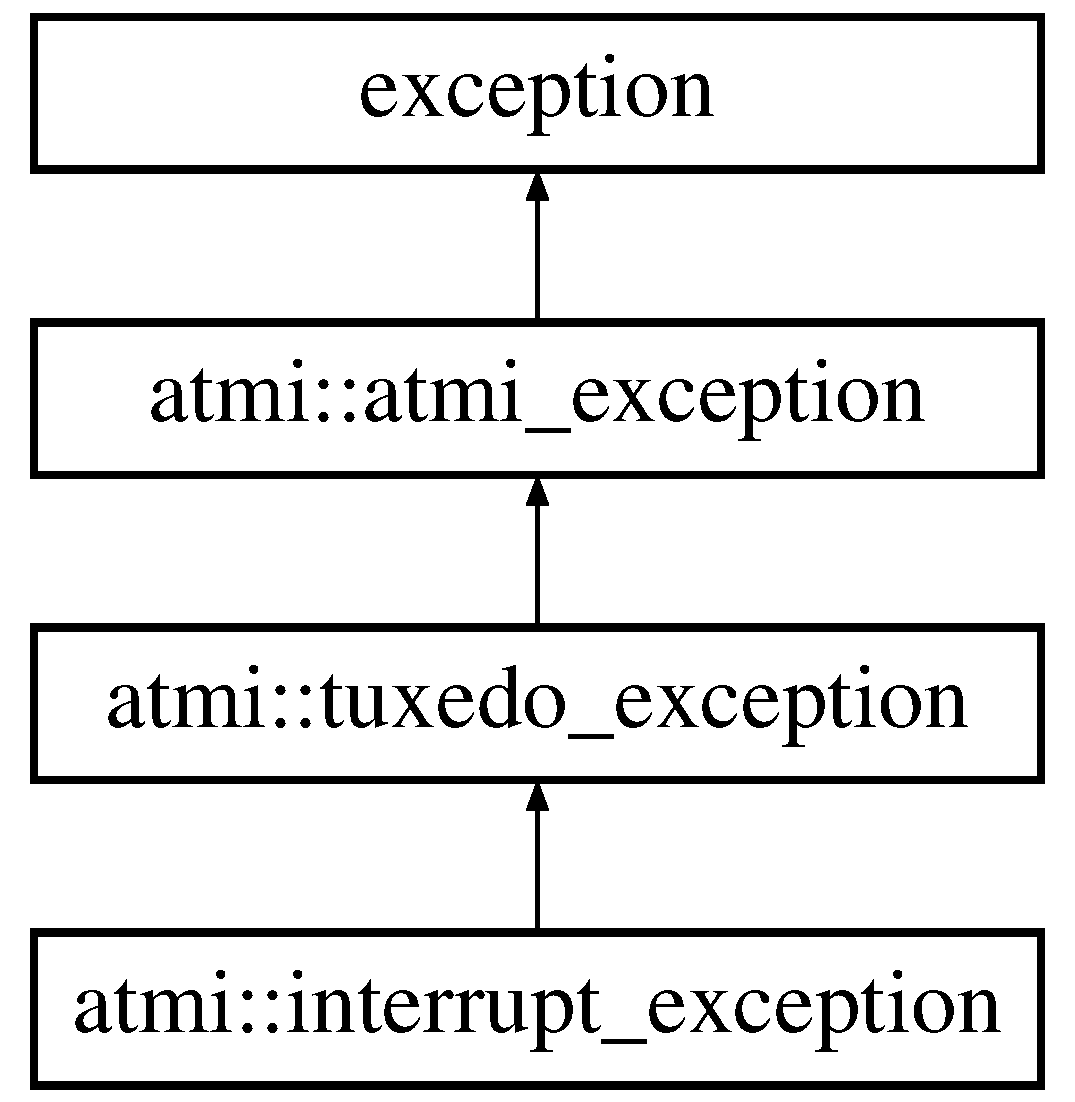
\includegraphics[height=4.000000cm]{classatmi_1_1interrupt__exception}
\end{center}
\end{figure}
\subsection*{Public Member Functions}
\begin{DoxyCompactItemize}
\item 
{\footnotesize template$<$typename... Args$>$ }\\\hyperlink{classatmi_1_1interrupt__exception_afe1b916f68a10fe0627f396052d45c9f}{interrupt\+\_\+exception} (const char $\ast$msg, const Args \&...args)
\end{DoxyCompactItemize}
\subsection*{Additional Inherited Members}


\subsection{Detailed Description}
Thrown when T\+P\+G\+O\+T\+S\+I\+G is returned after a signal was received. 

\subsection{Constructor \& Destructor Documentation}
\hypertarget{classatmi_1_1interrupt__exception_afe1b916f68a10fe0627f396052d45c9f}{\index{atmi\+::interrupt\+\_\+exception@{atmi\+::interrupt\+\_\+exception}!interrupt\+\_\+exception@{interrupt\+\_\+exception}}
\index{interrupt\+\_\+exception@{interrupt\+\_\+exception}!atmi\+::interrupt\+\_\+exception@{atmi\+::interrupt\+\_\+exception}}
\subsubsection[{interrupt\+\_\+exception}]{\setlength{\rightskip}{0pt plus 5cm}template$<$typename... Args$>$ atmi\+::interrupt\+\_\+exception\+::interrupt\+\_\+exception (
\begin{DoxyParamCaption}
\item[{const char $\ast$}]{msg, }
\item[{const Args \&...}]{args}
\end{DoxyParamCaption}
)\hspace{0.3cm}{\ttfamily [inline]}}}\label{classatmi_1_1interrupt__exception_afe1b916f68a10fe0627f396052d45c9f}
new instance.


\begin{DoxyParams}{Parameters}
{\em err} & Ferror32 value \\
\hline
{\em msg} & error message \\
\hline
{\em args} & error message parameters (variadic). \\
\hline
\end{DoxyParams}


The documentation for this class was generated from the following file\+:\begin{DoxyCompactItemize}
\item 
include/atmi/exceptions.\+hpp\end{DoxyCompactItemize}

\hypertarget{classatmi_1_1nomsg__exception}{}\section{atmi\+:\+:nomsg\+\_\+exception Class Reference}
\label{classatmi_1_1nomsg__exception}\index{atmi\+::nomsg\+\_\+exception@{atmi\+::nomsg\+\_\+exception}}


{\ttfamily \#include $<$exceptions.\+hpp$>$}

Inheritance diagram for atmi\+:\+:nomsg\+\_\+exception\+:\begin{figure}[H]
\begin{center}
\leavevmode
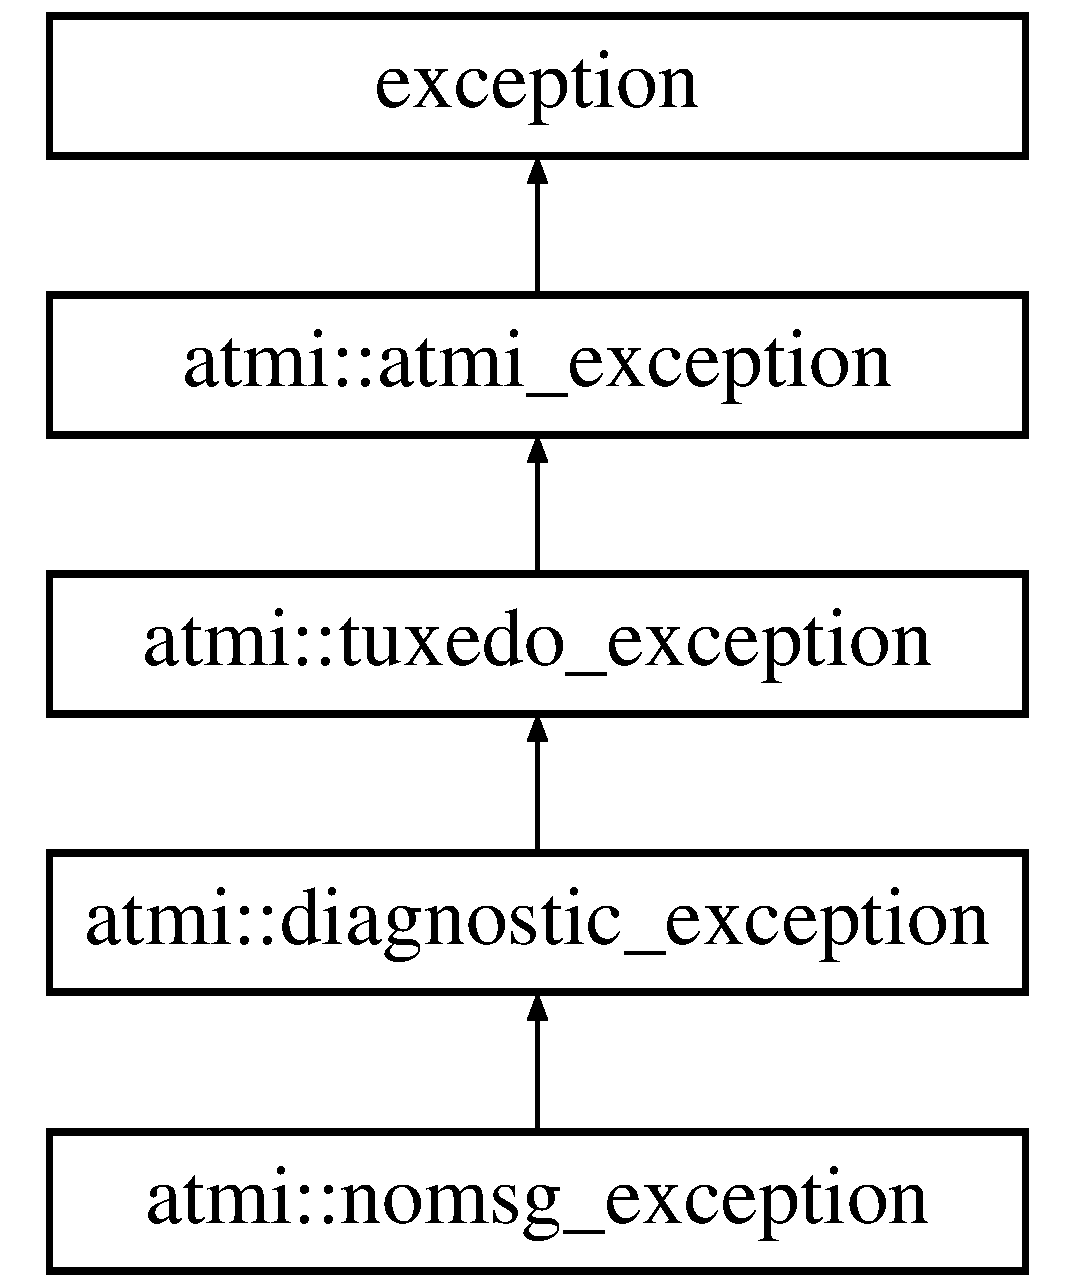
\includegraphics[height=5.000000cm]{classatmi_1_1nomsg__exception}
\end{center}
\end{figure}
\subsection*{Public Member Functions}
\begin{DoxyCompactItemize}
\item 
{\footnotesize template$<$typename... Args$>$ }\\\hyperlink{classatmi_1_1nomsg__exception_adf4039103c33fa16b63242cb7e129664}{nomsg\+\_\+exception} (const char $\ast$msg, const Args \&...args)
\end{DoxyCompactItemize}
\subsection*{Additional Inherited Members}


\subsection{Detailed Description}
Thrown when Q\+M\+E\+N\+O\+M\+S\+G is returned 

\subsection{Constructor \& Destructor Documentation}
\hypertarget{classatmi_1_1nomsg__exception_adf4039103c33fa16b63242cb7e129664}{}\index{atmi\+::nomsg\+\_\+exception@{atmi\+::nomsg\+\_\+exception}!nomsg\+\_\+exception@{nomsg\+\_\+exception}}
\index{nomsg\+\_\+exception@{nomsg\+\_\+exception}!atmi\+::nomsg\+\_\+exception@{atmi\+::nomsg\+\_\+exception}}
\subsubsection[{nomsg\+\_\+exception(const char $\ast$msg, const Args \&...\+args)}]{\setlength{\rightskip}{0pt plus 5cm}template$<$typename... Args$>$ atmi\+::nomsg\+\_\+exception\+::nomsg\+\_\+exception (
\begin{DoxyParamCaption}
\item[{const char $\ast$}]{msg, }
\item[{const Args \&...}]{args}
\end{DoxyParamCaption}
)\hspace{0.3cm}{\ttfamily [inline]}}\label{classatmi_1_1nomsg__exception_adf4039103c33fa16b63242cb7e129664}
Constructs a Queue exeption


\begin{DoxyParams}{Parameters}
{\em err} & value of tperr \\
\hline
{\em diagno} & value of ctl.\+diagnostic \\
\hline
{\em msg} & error message format. \\
\hline
{\em args} & error message parameters \\
\hline
\end{DoxyParams}


The documentation for this class was generated from the following file\+:\begin{DoxyCompactItemize}
\item 
include/atmi/exceptions.\+hpp\end{DoxyCompactItemize}

\hypertarget{classatmi_1_1queue}{\section{atmi\+:\+:queue Class Reference}
\label{classatmi_1_1queue}\index{atmi\+::queue@{atmi\+::queue}}
}


{\ttfamily \#include $<$queue.\+hpp$>$}

Inheritance diagram for atmi\+:\+:queue\+:\begin{figure}[H]
\begin{center}
\leavevmode
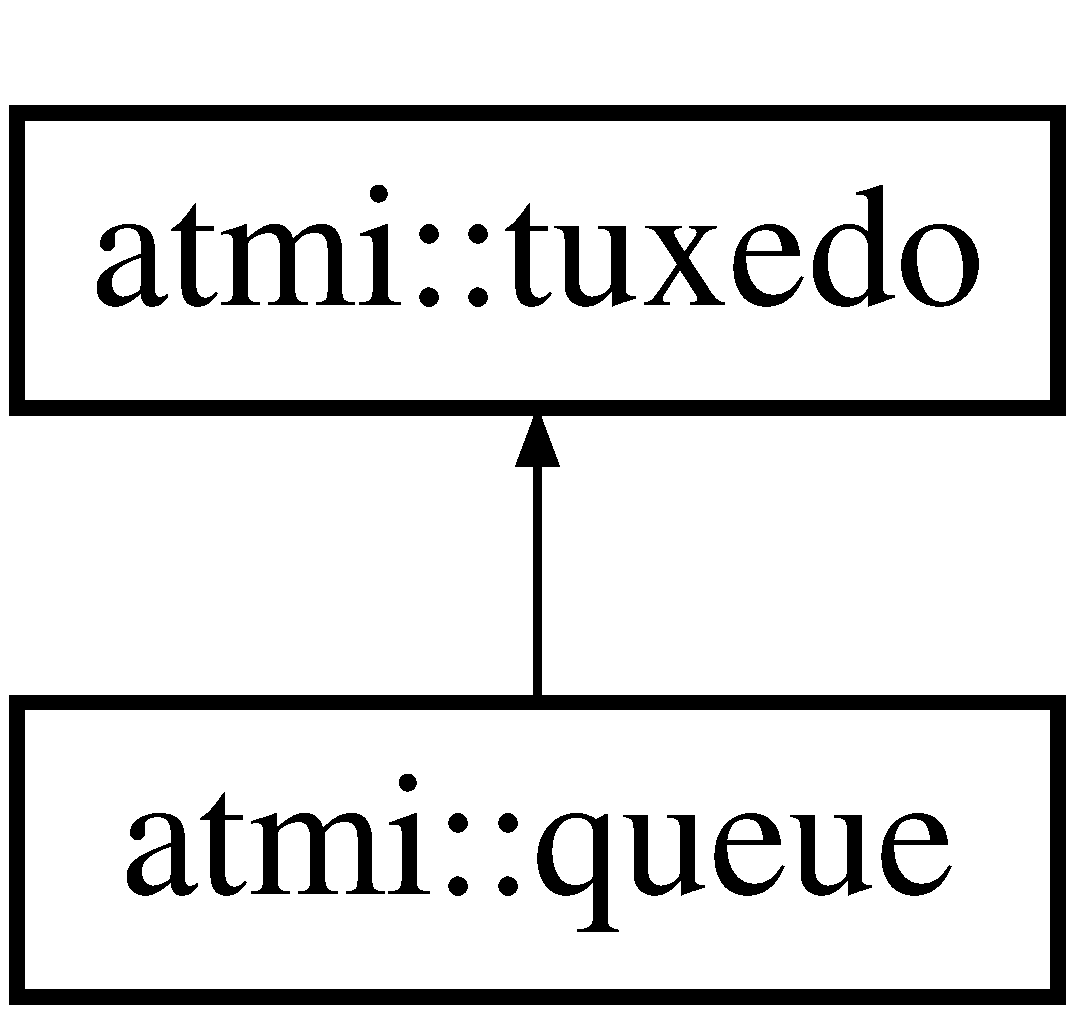
\includegraphics[height=2.000000cm]{classatmi_1_1queue}
\end{center}
\end{figure}
\subsection*{Public Member Functions}
\begin{DoxyCompactItemize}
\item 
\hyperlink{classatmi_1_1queue_af8c86b01e410fe6499a7f53cdf70eb35}{queue} (const char $\ast$qspace=N\+U\+L\+L, const char $\ast$\hyperlink{classatmi_1_1queue}{queue}=N\+U\+L\+L, const char $\ast$reply=N\+U\+L\+L)
\item 
int \hyperlink{classatmi_1_1queue_a6b27337fd68ca97236e4905d09b7eb15}{enqueue} (char $\ast$data, long len)
\item 
int \hyperlink{classatmi_1_1queue_a140e0faa2ab1265d3258ebc5f2049c41}{dequeue} (char $\ast$$\ast$data, long $\ast$len)
\item 
int \hyperlink{classatmi_1_1queue_a76cf5d92f7d727b0af48698cca6225c5}{enqueue} (\hyperlink{classatmi_1_1buffer}{buffer} \&data)
\item 
int \hyperlink{classatmi_1_1queue_a656e7c4acd4bfefdbecf098907020fad}{dequeue} (\hyperlink{classatmi_1_1buffer}{buffer} \&data)
\item 
int \hyperlink{classatmi_1_1queue_aa8a60e7609a1c28ec346a898a80f8ea6}{dequeue\+Reply} (char $\ast$$\ast$data, long $\ast$len)
\item 
int \hyperlink{classatmi_1_1queue_a1d0741ce63070da00a80cfc69db50797}{dequeue\+Reply} (\hyperlink{classatmi_1_1buffer}{buffer} \&data)
\item 
int \hyperlink{classatmi_1_1queue_a2ea608bb1f59fdccb2b7592381bcf267}{enqueue\+Reply} (char $\ast$data, long len)
\item 
int \hyperlink{classatmi_1_1queue_a2e04e4731abc851e48f6caf77ba61ef2}{enqueue\+Reply} (\hyperlink{classatmi_1_1buffer}{buffer} \&data)
\item 
void \hyperlink{classatmi_1_1queue_a216acfef7e80352c8ce8476825f1146e}{set\+\_\+reply\+\_\+queue} (const char $\ast$q)
\item 
const char $\ast$ \hyperlink{classatmi_1_1queue_ac851146259feb3bf93aed287d6d42cb2}{reply\+\_\+queue} ()
\item 
void \hyperlink{classatmi_1_1queue_a9b8f29fbb2012dda53d6f799ad2110b4}{set\+\_\+queue\+\_\+space} (const char $\ast$qs)
\item 
const char $\ast$ \hyperlink{classatmi_1_1queue_aaf7d8d18008f9ee987b7e7aa2195d1db}{queue\+\_\+space} ()
\item 
void \hyperlink{classatmi_1_1queue_a5d70bbf99076bd41269e2a558bf52475}{set\+\_\+queue\+\_\+name} (char $\ast$q)
\item 
const char $\ast$ \hyperlink{classatmi_1_1queue_adaddc33c75ec6e13f6c57da8d979ad32}{queue\+\_\+name} ()
\item 
long \hyperlink{classatmi_1_1queue_a96f51996c857985c9b8e1b720f726f0c}{qctl\+\_\+flags} ()
\item 
void \hyperlink{classatmi_1_1queue_a9669776889226a450093d2ddfd921d4b}{set\+\_\+message\+\_\+wait} (bool wait)
\item 
void \hyperlink{classatmi_1_1queue_a223fac7945fb8d87f04189aa77ce666a}{set\+Q\+Wait} (bool wait)
\item 
bool \hyperlink{classatmi_1_1queue_a90f5a71979755634b1e625d45ac61412}{is\+Q\+Waiting} ()
\item 
bool \hyperlink{classatmi_1_1queue_ac655db1db167f3e833f4fa84e6256428}{is\+\_\+message\+\_\+waiting} ()
\item 
void \hyperlink{classatmi_1_1queue_a0fbca137aadc2946b8f3889b76352af9}{set\+\_\+quality\+\_\+of\+\_\+service} (long qos)
\item 
int \hyperlink{classatmi_1_1queue_a1fabff1d9a56389a41f92542561d570d}{diagno} ()
\item 
void \hyperlink{classatmi_1_1queue_a2c0511c9f17e939789c5290fe83d1f1f}{set\+\_\+new\+\_\+corrid} ()
\item 
void \hyperlink{classatmi_1_1queue_aa74de8091c32580972e7871e7ddf786c}{unset\+\_\+corrid} ()
\end{DoxyCompactItemize}
\subsection*{Protected Member Functions}
\begin{DoxyCompactItemize}
\item 
{\footnotesize template$<$typename... Args$>$ }\\int \hyperlink{classatmi_1_1queue_a767f80e22a52d4b325d5a5aadc27a343}{handle\+\_\+diagnostics} (int tux\+\_\+tperrno, int tux\+\_\+diagno, const char $\ast$msg, const Args \&...args)
\end{DoxyCompactItemize}
\subsection*{Additional Inherited Members}


\subsection{Detailed Description}
Handles /\+Q operations 

\subsection{Constructor \& Destructor Documentation}
\hypertarget{classatmi_1_1queue_af8c86b01e410fe6499a7f53cdf70eb35}{\index{atmi\+::queue@{atmi\+::queue}!queue@{queue}}
\index{queue@{queue}!atmi\+::queue@{atmi\+::queue}}
\subsubsection[{queue}]{\setlength{\rightskip}{0pt plus 5cm}atmi\+::queue\+::queue (
\begin{DoxyParamCaption}
\item[{const char $\ast$}]{qspace = {\ttfamily NULL}, }
\item[{const char $\ast$}]{queue = {\ttfamily NULL}, }
\item[{const char $\ast$}]{reply = {\ttfamily NULL}}
\end{DoxyParamCaption}
)}}\label{classatmi_1_1queue_af8c86b01e410fe6499a7f53cdf70eb35}
Creates an instance of queue


\begin{DoxyParams}{Parameters}
{\em qspace} & qspace that handles the queue \\
\hline
{\em queue} & the queue that will be manipulated \\
\hline
{\em reply} & name of a reply \\
\hline
\end{DoxyParams}


\subsection{Member Function Documentation}
\hypertarget{classatmi_1_1queue_a140e0faa2ab1265d3258ebc5f2049c41}{\index{atmi\+::queue@{atmi\+::queue}!dequeue@{dequeue}}
\index{dequeue@{dequeue}!atmi\+::queue@{atmi\+::queue}}
\subsubsection[{dequeue}]{\setlength{\rightskip}{0pt plus 5cm}int atmi\+::queue\+::dequeue (
\begin{DoxyParamCaption}
\item[{char $\ast$$\ast$}]{data, }
\item[{long $\ast$}]{len}
\end{DoxyParamCaption}
)}}\label{classatmi_1_1queue_a140e0faa2ab1265d3258ebc5f2049c41}
dequeue a message


\begin{DoxyParams}{Parameters}
{\em data} & tuxedo buffer (allocated with \hyperlink{classatmi_1_1tuxedo_a44e77e3e6216a8c3fb8be33d5d8fed93}{tuxedo\+::allocate}) \\
\hline
{\em len} & length of the tuxedo buffer \\
\hline
\end{DoxyParams}
\hypertarget{classatmi_1_1queue_a656e7c4acd4bfefdbecf098907020fad}{\index{atmi\+::queue@{atmi\+::queue}!dequeue@{dequeue}}
\index{dequeue@{dequeue}!atmi\+::queue@{atmi\+::queue}}
\subsubsection[{dequeue}]{\setlength{\rightskip}{0pt plus 5cm}int atmi\+::queue\+::dequeue (
\begin{DoxyParamCaption}
\item[{{\bf buffer} \&}]{data}
\end{DoxyParamCaption}
)}}\label{classatmi_1_1queue_a656e7c4acd4bfefdbecf098907020fad}
dequeue a message


\begin{DoxyParams}{Parameters}
{\em data} & tuxedo F\+M\+L32 buffer (allocated with \hyperlink{classatmi_1_1tuxedo_a44e77e3e6216a8c3fb8be33d5d8fed93}{tuxedo\+::allocate}) \\
\hline
\end{DoxyParams}
\hypertarget{classatmi_1_1queue_aa8a60e7609a1c28ec346a898a80f8ea6}{\index{atmi\+::queue@{atmi\+::queue}!dequeue\+Reply@{dequeue\+Reply}}
\index{dequeue\+Reply@{dequeue\+Reply}!atmi\+::queue@{atmi\+::queue}}
\subsubsection[{dequeue\+Reply}]{\setlength{\rightskip}{0pt plus 5cm}int atmi\+::queue\+::dequeue\+Reply (
\begin{DoxyParamCaption}
\item[{char $\ast$$\ast$}]{data, }
\item[{long $\ast$}]{len}
\end{DoxyParamCaption}
)}}\label{classatmi_1_1queue_aa8a60e7609a1c28ec346a898a80f8ea6}
dequeue a reply message

Reply must have been set when queue instance was created. If the flag T\+P T\+P\+Q\+C\+O\+R\+R\+I\+D is set, then the correlation id value is used to retreive the message from the reply queue.


\begin{DoxyParams}{Parameters}
{\em data} & tuxedo buffer (allocated with \hyperlink{classatmi_1_1tuxedo_a44e77e3e6216a8c3fb8be33d5d8fed93}{tuxedo\+::allocate}) \\
\hline
{\em len} & length of the tuxedo buffer \\
\hline
\end{DoxyParams}
\hypertarget{classatmi_1_1queue_a1d0741ce63070da00a80cfc69db50797}{\index{atmi\+::queue@{atmi\+::queue}!dequeue\+Reply@{dequeue\+Reply}}
\index{dequeue\+Reply@{dequeue\+Reply}!atmi\+::queue@{atmi\+::queue}}
\subsubsection[{dequeue\+Reply}]{\setlength{\rightskip}{0pt plus 5cm}int atmi\+::queue\+::dequeue\+Reply (
\begin{DoxyParamCaption}
\item[{{\bf buffer} \&}]{data}
\end{DoxyParamCaption}
)}}\label{classatmi_1_1queue_a1d0741ce63070da00a80cfc69db50797}
dequeue a reply message

Reply must have been set when queue instance was created.


\begin{DoxyParams}{Parameters}
{\em data} & tuxedo buffer (allocated with \hyperlink{classatmi_1_1tuxedo_a44e77e3e6216a8c3fb8be33d5d8fed93}{tuxedo\+::allocate}) \\
\hline
\end{DoxyParams}
\hypertarget{classatmi_1_1queue_a1fabff1d9a56389a41f92542561d570d}{\index{atmi\+::queue@{atmi\+::queue}!diagno@{diagno}}
\index{diagno@{diagno}!atmi\+::queue@{atmi\+::queue}}
\subsubsection[{diagno}]{\setlength{\rightskip}{0pt plus 5cm}int atmi\+::queue\+::diagno (
\begin{DoxyParamCaption}
{}
\end{DoxyParamCaption}
)\hspace{0.3cm}{\ttfamily [inline]}}}\label{classatmi_1_1queue_a1fabff1d9a56389a41f92542561d570d}
\begin{DoxyReturn}{Returns}
the diagnostic code returned by last call. 
\end{DoxyReturn}
\hypertarget{classatmi_1_1queue_a6b27337fd68ca97236e4905d09b7eb15}{\index{atmi\+::queue@{atmi\+::queue}!enqueue@{enqueue}}
\index{enqueue@{enqueue}!atmi\+::queue@{atmi\+::queue}}
\subsubsection[{enqueue}]{\setlength{\rightskip}{0pt plus 5cm}int atmi\+::queue\+::enqueue (
\begin{DoxyParamCaption}
\item[{char $\ast$}]{data, }
\item[{long}]{len}
\end{DoxyParamCaption}
)}}\label{classatmi_1_1queue_a6b27337fd68ca97236e4905d09b7eb15}
enqueue a message


\begin{DoxyParams}{Parameters}
{\em data} & tuxedo buffer (allocated with \hyperlink{classatmi_1_1tuxedo_a44e77e3e6216a8c3fb8be33d5d8fed93}{tuxedo\+::allocate}) \\
\hline
{\em len} & length of the tuxedo buffer \\
\hline
\end{DoxyParams}
\hypertarget{classatmi_1_1queue_a76cf5d92f7d727b0af48698cca6225c5}{\index{atmi\+::queue@{atmi\+::queue}!enqueue@{enqueue}}
\index{enqueue@{enqueue}!atmi\+::queue@{atmi\+::queue}}
\subsubsection[{enqueue}]{\setlength{\rightskip}{0pt plus 5cm}int atmi\+::queue\+::enqueue (
\begin{DoxyParamCaption}
\item[{{\bf buffer} \&}]{data}
\end{DoxyParamCaption}
)}}\label{classatmi_1_1queue_a76cf5d92f7d727b0af48698cca6225c5}
enqueue a message


\begin{DoxyParams}{Parameters}
{\em data} & tuxedo F\+M\+L32 buffer (allocated with \hyperlink{classatmi_1_1tuxedo_a44e77e3e6216a8c3fb8be33d5d8fed93}{tuxedo\+::allocate}) \\
\hline
\end{DoxyParams}
\hypertarget{classatmi_1_1queue_a2ea608bb1f59fdccb2b7592381bcf267}{\index{atmi\+::queue@{atmi\+::queue}!enqueue\+Reply@{enqueue\+Reply}}
\index{enqueue\+Reply@{enqueue\+Reply}!atmi\+::queue@{atmi\+::queue}}
\subsubsection[{enqueue\+Reply}]{\setlength{\rightskip}{0pt plus 5cm}int atmi\+::queue\+::enqueue\+Reply (
\begin{DoxyParamCaption}
\item[{char $\ast$}]{data, }
\item[{long}]{len}
\end{DoxyParamCaption}
)}}\label{classatmi_1_1queue_a2ea608bb1f59fdccb2b7592381bcf267}
enqueue a reply message

The reply queue is identified through the Qctl structure. It is the responability of the caller to set the reply queue value to use.


\begin{DoxyParams}{Parameters}
{\em data} & tuxedo buffer (allocated with \hyperlink{classatmi_1_1tuxedo_a44e77e3e6216a8c3fb8be33d5d8fed93}{tuxedo\+::allocate}) \\
\hline
{\em len} & length of the tuxedo buffer \\
\hline
\end{DoxyParams}
\hypertarget{classatmi_1_1queue_a2e04e4731abc851e48f6caf77ba61ef2}{\index{atmi\+::queue@{atmi\+::queue}!enqueue\+Reply@{enqueue\+Reply}}
\index{enqueue\+Reply@{enqueue\+Reply}!atmi\+::queue@{atmi\+::queue}}
\subsubsection[{enqueue\+Reply}]{\setlength{\rightskip}{0pt plus 5cm}int atmi\+::queue\+::enqueue\+Reply (
\begin{DoxyParamCaption}
\item[{{\bf buffer} \&}]{data}
\end{DoxyParamCaption}
)}}\label{classatmi_1_1queue_a2e04e4731abc851e48f6caf77ba61ef2}
enqueue a reply message

The reply queue is identified through the Qctl structure. It is the responability of the caller to set the reply queue value to use.


\begin{DoxyParams}{Parameters}
{\em data} & tuxedo buffer (allocated with \hyperlink{classatmi_1_1tuxedo_a44e77e3e6216a8c3fb8be33d5d8fed93}{tuxedo\+::allocate}) \\
\hline
\end{DoxyParams}
\hypertarget{classatmi_1_1queue_a767f80e22a52d4b325d5a5aadc27a343}{\index{atmi\+::queue@{atmi\+::queue}!handle\+\_\+diagnostics@{handle\+\_\+diagnostics}}
\index{handle\+\_\+diagnostics@{handle\+\_\+diagnostics}!atmi\+::queue@{atmi\+::queue}}
\subsubsection[{handle\+\_\+diagnostics}]{\setlength{\rightskip}{0pt plus 5cm}template$<$typename... Args$>$ int atmi\+::queue\+::handle\+\_\+diagnostics (
\begin{DoxyParamCaption}
\item[{int}]{tux\+\_\+tperrno, }
\item[{int}]{tux\+\_\+diagno, }
\item[{const char $\ast$}]{msg, }
\item[{const Args \&...}]{args}
\end{DoxyParamCaption}
)\hspace{0.3cm}{\ttfamily [inline]}, {\ttfamily [protected]}}}\label{classatmi_1_1queue_a767f80e22a52d4b325d5a5aadc27a343}
handle queue diagnostic errors


\begin{DoxyParams}{Parameters}
{\em tux\+\_\+tperrno} & tperrno to handle \\
\hline
{\em tux\+\_\+diagno} & diagnostic number \\
\hline
{\em msg} & related explanatory message. \\
\hline
{\em args} & message arguments \\
\hline
\end{DoxyParams}
\hypertarget{classatmi_1_1queue_ac655db1db167f3e833f4fa84e6256428}{\index{atmi\+::queue@{atmi\+::queue}!is\+\_\+message\+\_\+waiting@{is\+\_\+message\+\_\+waiting}}
\index{is\+\_\+message\+\_\+waiting@{is\+\_\+message\+\_\+waiting}!atmi\+::queue@{atmi\+::queue}}
\subsubsection[{is\+\_\+message\+\_\+waiting}]{\setlength{\rightskip}{0pt plus 5cm}bool atmi\+::queue\+::is\+\_\+message\+\_\+waiting (
\begin{DoxyParamCaption}
{}
\end{DoxyParamCaption}
)\hspace{0.3cm}{\ttfamily [inline]}}}\label{classatmi_1_1queue_ac655db1db167f3e833f4fa84e6256428}
\begin{DoxyReturn}{Returns}
ture if T\+P\+Q\+W\+A\+I\+T flag is set. 
\end{DoxyReturn}
\hypertarget{classatmi_1_1queue_a90f5a71979755634b1e625d45ac61412}{\index{atmi\+::queue@{atmi\+::queue}!is\+Q\+Waiting@{is\+Q\+Waiting}}
\index{is\+Q\+Waiting@{is\+Q\+Waiting}!atmi\+::queue@{atmi\+::queue}}
\subsubsection[{is\+Q\+Waiting}]{\setlength{\rightskip}{0pt plus 5cm}bool atmi\+::queue\+::is\+Q\+Waiting (
\begin{DoxyParamCaption}
{}
\end{DoxyParamCaption}
)\hspace{0.3cm}{\ttfamily [inline]}}}\label{classatmi_1_1queue_a90f5a71979755634b1e625d45ac61412}
Check if Q\+Wait flag is set

\begin{DoxyReturn}{Returns}
true if wait flag is set 
\end{DoxyReturn}
\begin{DoxyRefDesc}{Deprecated}
\item[\hyperlink{deprecated__deprecated000004}{Deprecated}]use is\+\_\+message\+\_\+waiting instead \end{DoxyRefDesc}
\hypertarget{classatmi_1_1queue_a96f51996c857985c9b8e1b720f726f0c}{\index{atmi\+::queue@{atmi\+::queue}!qctl\+\_\+flags@{qctl\+\_\+flags}}
\index{qctl\+\_\+flags@{qctl\+\_\+flags}!atmi\+::queue@{atmi\+::queue}}
\subsubsection[{qctl\+\_\+flags}]{\setlength{\rightskip}{0pt plus 5cm}long atmi\+::queue\+::qctl\+\_\+flags (
\begin{DoxyParamCaption}
{}
\end{DoxyParamCaption}
)\hspace{0.3cm}{\ttfamily [inline]}}}\label{classatmi_1_1queue_a96f51996c857985c9b8e1b720f726f0c}
\begin{DoxyReturn}{Returns}
the current value of Q\+C\+T\+L flags 
\end{DoxyReturn}
\hypertarget{classatmi_1_1queue_adaddc33c75ec6e13f6c57da8d979ad32}{\index{atmi\+::queue@{atmi\+::queue}!queue\+\_\+name@{queue\+\_\+name}}
\index{queue\+\_\+name@{queue\+\_\+name}!atmi\+::queue@{atmi\+::queue}}
\subsubsection[{queue\+\_\+name}]{\setlength{\rightskip}{0pt plus 5cm}const char$\ast$ atmi\+::queue\+::queue\+\_\+name (
\begin{DoxyParamCaption}
{}
\end{DoxyParamCaption}
)\hspace{0.3cm}{\ttfamily [inline]}}}\label{classatmi_1_1queue_adaddc33c75ec6e13f6c57da8d979ad32}
\begin{DoxyReturn}{Returns}
the currently wrapped queue name 
\end{DoxyReturn}
\hypertarget{classatmi_1_1queue_aaf7d8d18008f9ee987b7e7aa2195d1db}{\index{atmi\+::queue@{atmi\+::queue}!queue\+\_\+space@{queue\+\_\+space}}
\index{queue\+\_\+space@{queue\+\_\+space}!atmi\+::queue@{atmi\+::queue}}
\subsubsection[{queue\+\_\+space}]{\setlength{\rightskip}{0pt plus 5cm}const char$\ast$ atmi\+::queue\+::queue\+\_\+space (
\begin{DoxyParamCaption}
{}
\end{DoxyParamCaption}
)\hspace{0.3cm}{\ttfamily [inline]}}}\label{classatmi_1_1queue_aaf7d8d18008f9ee987b7e7aa2195d1db}
\begin{DoxyReturn}{Returns}
queue's queque space name 
\end{DoxyReturn}
\hypertarget{classatmi_1_1queue_ac851146259feb3bf93aed287d6d42cb2}{\index{atmi\+::queue@{atmi\+::queue}!reply\+\_\+queue@{reply\+\_\+queue}}
\index{reply\+\_\+queue@{reply\+\_\+queue}!atmi\+::queue@{atmi\+::queue}}
\subsubsection[{reply\+\_\+queue}]{\setlength{\rightskip}{0pt plus 5cm}const char $\ast$ atmi\+::queue\+::reply\+\_\+queue (
\begin{DoxyParamCaption}
{}
\end{DoxyParamCaption}
)}}\label{classatmi_1_1queue_ac851146259feb3bf93aed287d6d42cb2}
reply message are expected to be posted onto this /\+Q queue.

\begin{DoxyReturn}{Returns}
reply queue name 
\end{DoxyReturn}
\hypertarget{classatmi_1_1queue_a9669776889226a450093d2ddfd921d4b}{\index{atmi\+::queue@{atmi\+::queue}!set\+\_\+message\+\_\+wait@{set\+\_\+message\+\_\+wait}}
\index{set\+\_\+message\+\_\+wait@{set\+\_\+message\+\_\+wait}!atmi\+::queue@{atmi\+::queue}}
\subsubsection[{set\+\_\+message\+\_\+wait}]{\setlength{\rightskip}{0pt plus 5cm}void atmi\+::queue\+::set\+\_\+message\+\_\+wait (
\begin{DoxyParamCaption}
\item[{bool}]{wait}
\end{DoxyParamCaption}
)}}\label{classatmi_1_1queue_a9669776889226a450093d2ddfd921d4b}
Wait until a message is enqueued.


\begin{DoxyParams}{Parameters}
{\em wait} & if true queue waits for a message \\
\hline
\end{DoxyParams}
\hypertarget{classatmi_1_1queue_a2c0511c9f17e939789c5290fe83d1f1f}{\index{atmi\+::queue@{atmi\+::queue}!set\+\_\+new\+\_\+corrid@{set\+\_\+new\+\_\+corrid}}
\index{set\+\_\+new\+\_\+corrid@{set\+\_\+new\+\_\+corrid}!atmi\+::queue@{atmi\+::queue}}
\subsubsection[{set\+\_\+new\+\_\+corrid}]{\setlength{\rightskip}{0pt plus 5cm}void atmi\+::queue\+::set\+\_\+new\+\_\+corrid (
\begin{DoxyParamCaption}
{}
\end{DoxyParamCaption}
)}}\label{classatmi_1_1queue_a2c0511c9f17e939789c5290fe83d1f1f}
Calculate and set qctl corid

Correlation I\+D is made of pid+threadid+current\+\_\+time (in milliseconds). When the correlation is set the flags T\+P\+Q\+G\+E\+T\+B\+Y\+C\+O\+R\+R\+I\+D and T\+P\+Q\+C\+O\+R\+R\+I\+D are also set. This means that subsequent calls to dequeue methods will get only message with the correleation id that was last set. \hypertarget{classatmi_1_1queue_a0fbca137aadc2946b8f3889b76352af9}{\index{atmi\+::queue@{atmi\+::queue}!set\+\_\+quality\+\_\+of\+\_\+service@{set\+\_\+quality\+\_\+of\+\_\+service}}
\index{set\+\_\+quality\+\_\+of\+\_\+service@{set\+\_\+quality\+\_\+of\+\_\+service}!atmi\+::queue@{atmi\+::queue}}
\subsubsection[{set\+\_\+quality\+\_\+of\+\_\+service}]{\setlength{\rightskip}{0pt plus 5cm}void atmi\+::queue\+::set\+\_\+quality\+\_\+of\+\_\+service (
\begin{DoxyParamCaption}
\item[{long}]{qos}
\end{DoxyParamCaption}
)}}\label{classatmi_1_1queue_a0fbca137aadc2946b8f3889b76352af9}
Set the desired persistence mode (memory, disk, default) Accepted values are \+: T\+P\+Q\+Q\+O\+S\+D\+E\+F\+A\+U\+L\+T\+P\+E\+R\+S\+I\+S\+T\+: uses the persistence mode defined with queue T\+P\+Q\+Q\+O\+S\+P\+E\+R\+S\+I\+S\+T\+E\+N\+T\+: message are written onto persistent storage T\+P\+Q\+Q\+O\+S\+N\+O\+N\+P\+E\+R\+S\+I\+S\+T\+E\+N\+T\+: message are written into memory only (message are lost if the queue manager is interrupted)


\begin{DoxyParams}{Parameters}
{\em qos} & desired flags \\
\hline
\end{DoxyParams}
\hypertarget{classatmi_1_1queue_a5d70bbf99076bd41269e2a558bf52475}{\index{atmi\+::queue@{atmi\+::queue}!set\+\_\+queue\+\_\+name@{set\+\_\+queue\+\_\+name}}
\index{set\+\_\+queue\+\_\+name@{set\+\_\+queue\+\_\+name}!atmi\+::queue@{atmi\+::queue}}
\subsubsection[{set\+\_\+queue\+\_\+name}]{\setlength{\rightskip}{0pt plus 5cm}void atmi\+::queue\+::set\+\_\+queue\+\_\+name (
\begin{DoxyParamCaption}
\item[{char $\ast$}]{q}
\end{DoxyParamCaption}
)\hspace{0.3cm}{\ttfamily [inline]}}}\label{classatmi_1_1queue_a5d70bbf99076bd41269e2a558bf52475}
set the queue the instance is wrapping.


\begin{DoxyParams}{Parameters}
{\em q} & queue name \\
\hline
\end{DoxyParams}
\begin{DoxySeeAlso}{See also}
\hyperlink{classatmi_1_1queue_a9b8f29fbb2012dda53d6f799ad2110b4}{set\+\_\+queue\+\_\+space} make sure the \hyperlink{classatmi_1_1queue}{queue} name exists in the current \hyperlink{classatmi_1_1queue}{queue} space. 
\end{DoxySeeAlso}
\hypertarget{classatmi_1_1queue_a9b8f29fbb2012dda53d6f799ad2110b4}{\index{atmi\+::queue@{atmi\+::queue}!set\+\_\+queue\+\_\+space@{set\+\_\+queue\+\_\+space}}
\index{set\+\_\+queue\+\_\+space@{set\+\_\+queue\+\_\+space}!atmi\+::queue@{atmi\+::queue}}
\subsubsection[{set\+\_\+queue\+\_\+space}]{\setlength{\rightskip}{0pt plus 5cm}void atmi\+::queue\+::set\+\_\+queue\+\_\+space (
\begin{DoxyParamCaption}
\item[{const char $\ast$}]{qs}
\end{DoxyParamCaption}
)\hspace{0.3cm}{\ttfamily [inline]}}}\label{classatmi_1_1queue_a9b8f29fbb2012dda53d6f799ad2110b4}
Set the queuespace name to wich this queue associated.


\begin{DoxyParams}{Parameters}
{\em qs} & queue space name (32 characters max) \\
\hline
\end{DoxyParams}
\hypertarget{classatmi_1_1queue_a216acfef7e80352c8ce8476825f1146e}{\index{atmi\+::queue@{atmi\+::queue}!set\+\_\+reply\+\_\+queue@{set\+\_\+reply\+\_\+queue}}
\index{set\+\_\+reply\+\_\+queue@{set\+\_\+reply\+\_\+queue}!atmi\+::queue@{atmi\+::queue}}
\subsubsection[{set\+\_\+reply\+\_\+queue}]{\setlength{\rightskip}{0pt plus 5cm}void atmi\+::queue\+::set\+\_\+reply\+\_\+queue (
\begin{DoxyParamCaption}
\item[{const char $\ast$}]{q}
\end{DoxyParamCaption}
)}}\label{classatmi_1_1queue_a216acfef7e80352c8ce8476825f1146e}
indicate in wich queue the replies should be posted in.


\begin{DoxyParams}{Parameters}
{\em q} & reply queue, if N\+U\+L\+L then current reply queue is unset. \\
\hline
\end{DoxyParams}
\hypertarget{classatmi_1_1queue_a223fac7945fb8d87f04189aa77ce666a}{\index{atmi\+::queue@{atmi\+::queue}!set\+Q\+Wait@{set\+Q\+Wait}}
\index{set\+Q\+Wait@{set\+Q\+Wait}!atmi\+::queue@{atmi\+::queue}}
\subsubsection[{set\+Q\+Wait}]{\setlength{\rightskip}{0pt plus 5cm}void atmi\+::queue\+::set\+Q\+Wait (
\begin{DoxyParamCaption}
\item[{bool}]{wait}
\end{DoxyParamCaption}
)\hspace{0.3cm}{\ttfamily [inline]}}}\label{classatmi_1_1queue_a223fac7945fb8d87f04189aa77ce666a}
\begin{DoxyRefDesc}{Deprecated}
\item[\hyperlink{deprecated__deprecated000003}{Deprecated}]use set\+\_\+message\+\_\+wait instead \end{DoxyRefDesc}
\hypertarget{classatmi_1_1queue_aa74de8091c32580972e7871e7ddf786c}{\index{atmi\+::queue@{atmi\+::queue}!unset\+\_\+corrid@{unset\+\_\+corrid}}
\index{unset\+\_\+corrid@{unset\+\_\+corrid}!atmi\+::queue@{atmi\+::queue}}
\subsubsection[{unset\+\_\+corrid}]{\setlength{\rightskip}{0pt plus 5cm}void atmi\+::queue\+::unset\+\_\+corrid (
\begin{DoxyParamCaption}
{}
\end{DoxyParamCaption}
)}}\label{classatmi_1_1queue_aa74de8091c32580972e7871e7ddf786c}
Reset flags and value related to correlation id to off. 

The documentation for this class was generated from the following files\+:\begin{DoxyCompactItemize}
\item 
include/atmi/queue.\+hpp\item 
src/queue.\+cpp\end{DoxyCompactItemize}

\hypertarget{classatmi_1_1queue__stream}{\section{atmi\+:\+:queue\+\_\+stream Class Reference}
\label{classatmi_1_1queue__stream}\index{atmi\+::queue\+\_\+stream@{atmi\+::queue\+\_\+stream}}
}


{\ttfamily \#include $<$tuxedo.\+hpp$>$}

Inheritance diagram for atmi\+:\+:queue\+\_\+stream\+:\begin{figure}[H]
\begin{center}
\leavevmode
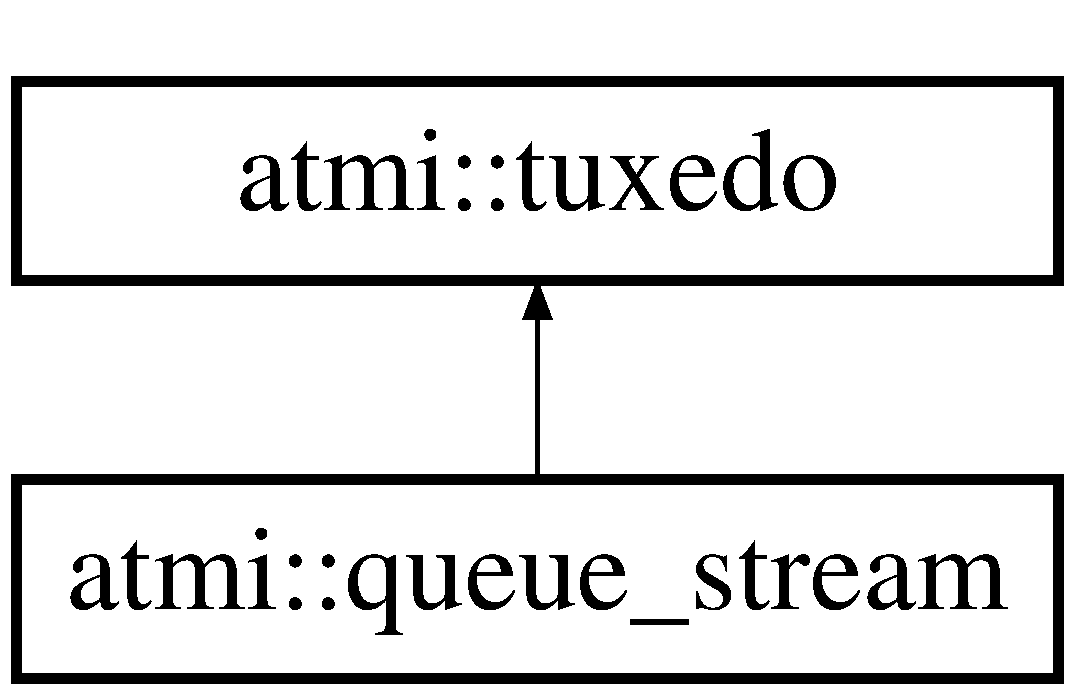
\includegraphics[height=2.000000cm]{classatmi_1_1queue__stream}
\end{center}
\end{figure}
\subsection*{Public Member Functions}
\begin{DoxyCompactItemize}
\item 
\hyperlink{classatmi_1_1queue__stream_a775623d6cd91a8a3cd40d9bb1e492c60}{queue\+\_\+stream} (\hyperlink{classatmi_1_1queue}{queue} $\ast$q)
\item 
\hyperlink{classatmi_1_1queue__stream_af05f48449db9ed2282643d9e7c148944}{queue\+\_\+stream} (\hyperlink{classatmi_1_1queue}{queue} $\ast$q, long bs)
\item 
long \hyperlink{classatmi_1_1queue__stream_ac4f1e88530a4d9fda0bc4b271301866b}{count} ()
\item 
void \hyperlink{classatmi_1_1queue__stream_a500b658e3f3f1a353982a1304ea27801}{set\+\_\+buffer\+\_\+size} (long s)
\item 
long \hyperlink{classatmi_1_1queue__stream_a18d01411c5ffeffd190195fd2b4dc61a}{buffer\+\_\+size} ()
\item 
void \hyperlink{classatmi_1_1queue__stream_a4a47e7caf329e46c31f44425e3ceb6e3}{encode\+\_\+base64} (bool b)
\end{DoxyCompactItemize}
\subsection*{Friends}
\begin{DoxyCompactItemize}
\item 
ostream \& \hyperlink{classatmi_1_1queue__stream_ad655c66351739698af3d404de31d3179}{operator$<$$<$} (ostream \&out, \hyperlink{classatmi_1_1queue__stream}{queue\+\_\+stream} \&qs)
\item 
istream \& \hyperlink{classatmi_1_1queue__stream_a52e264f6a625c0a453157abc46da7efe}{operator$>$$>$} (istream \&in, \hyperlink{classatmi_1_1queue__stream}{queue\+\_\+stream} \&qs)
\end{DoxyCompactItemize}
\subsection*{Additional Inherited Members}


\subsection{Detailed Description}
Handles in/out operation on a queue 

\subsection{Constructor \& Destructor Documentation}
\hypertarget{classatmi_1_1queue__stream_a775623d6cd91a8a3cd40d9bb1e492c60}{\index{atmi\+::queue\+\_\+stream@{atmi\+::queue\+\_\+stream}!queue\+\_\+stream@{queue\+\_\+stream}}
\index{queue\+\_\+stream@{queue\+\_\+stream}!atmi\+::queue\+\_\+stream@{atmi\+::queue\+\_\+stream}}
\subsubsection[{queue\+\_\+stream}]{\setlength{\rightskip}{0pt plus 5cm}atmi\+::queue\+\_\+stream\+::queue\+\_\+stream (
\begin{DoxyParamCaption}
\item[{{\bf atmi\+::queue} $\ast$}]{q}
\end{DoxyParamCaption}
)}}\label{classatmi_1_1queue__stream_a775623d6cd91a8a3cd40d9bb1e492c60}
setup a queue stream.


\begin{DoxyParams}{Parameters}
{\em q} & a queue \\
\hline
\end{DoxyParams}
\hypertarget{classatmi_1_1queue__stream_af05f48449db9ed2282643d9e7c148944}{\index{atmi\+::queue\+\_\+stream@{atmi\+::queue\+\_\+stream}!queue\+\_\+stream@{queue\+\_\+stream}}
\index{queue\+\_\+stream@{queue\+\_\+stream}!atmi\+::queue\+\_\+stream@{atmi\+::queue\+\_\+stream}}
\subsubsection[{queue\+\_\+stream}]{\setlength{\rightskip}{0pt plus 5cm}atmi\+::queue\+\_\+stream\+::queue\+\_\+stream (
\begin{DoxyParamCaption}
\item[{{\bf atmi\+::queue} $\ast$}]{queue, }
\item[{long}]{bs}
\end{DoxyParamCaption}
)}}\label{classatmi_1_1queue__stream_af05f48449db9ed2282643d9e7c148944}
setup a queue stream.


\begin{DoxyParams}{Parameters}
{\em q} & a queue \\
\hline
{\em bs} & stream buffer size. \\
\hline
\end{DoxyParams}


\subsection{Member Function Documentation}
\hypertarget{classatmi_1_1queue__stream_a18d01411c5ffeffd190195fd2b4dc61a}{\index{atmi\+::queue\+\_\+stream@{atmi\+::queue\+\_\+stream}!buffer\+\_\+size@{buffer\+\_\+size}}
\index{buffer\+\_\+size@{buffer\+\_\+size}!atmi\+::queue\+\_\+stream@{atmi\+::queue\+\_\+stream}}
\subsubsection[{buffer\+\_\+size}]{\setlength{\rightskip}{0pt plus 5cm}long atmi\+::queue\+\_\+stream\+::buffer\+\_\+size (
\begin{DoxyParamCaption}
{}
\end{DoxyParamCaption}
)\hspace{0.3cm}{\ttfamily [inline]}}}\label{classatmi_1_1queue__stream_a18d01411c5ffeffd190195fd2b4dc61a}
\begin{DoxyReturn}{Returns}
current buffer size 
\end{DoxyReturn}
\hypertarget{classatmi_1_1queue__stream_ac4f1e88530a4d9fda0bc4b271301866b}{\index{atmi\+::queue\+\_\+stream@{atmi\+::queue\+\_\+stream}!count@{count}}
\index{count@{count}!atmi\+::queue\+\_\+stream@{atmi\+::queue\+\_\+stream}}
\subsubsection[{count}]{\setlength{\rightskip}{0pt plus 5cm}long atmi\+::queue\+\_\+stream\+::count (
\begin{DoxyParamCaption}
{}
\end{DoxyParamCaption}
)\hspace{0.3cm}{\ttfamily [inline]}}}\label{classatmi_1_1queue__stream_ac4f1e88530a4d9fda0bc4b271301866b}
\begin{DoxyReturn}{Returns}
the number of messages handle by last I\+O operation 
\end{DoxyReturn}
\hypertarget{classatmi_1_1queue__stream_a4a47e7caf329e46c31f44425e3ceb6e3}{\index{atmi\+::queue\+\_\+stream@{atmi\+::queue\+\_\+stream}!encode\+\_\+base64@{encode\+\_\+base64}}
\index{encode\+\_\+base64@{encode\+\_\+base64}!atmi\+::queue\+\_\+stream@{atmi\+::queue\+\_\+stream}}
\subsubsection[{encode\+\_\+base64}]{\setlength{\rightskip}{0pt plus 5cm}void atmi\+::queue\+\_\+stream\+::encode\+\_\+base64 (
\begin{DoxyParamCaption}
\item[{bool}]{b}
\end{DoxyParamCaption}
)}}\label{classatmi_1_1queue__stream_a4a47e7caf329e46c31f44425e3ceb6e3}
use base64 encoding 
\begin{DoxyParams}{Parameters}
{\em b} & if true, the encode using base64 \\
\hline
\end{DoxyParams}
\hypertarget{classatmi_1_1queue__stream_a500b658e3f3f1a353982a1304ea27801}{\index{atmi\+::queue\+\_\+stream@{atmi\+::queue\+\_\+stream}!set\+\_\+buffer\+\_\+size@{set\+\_\+buffer\+\_\+size}}
\index{set\+\_\+buffer\+\_\+size@{set\+\_\+buffer\+\_\+size}!atmi\+::queue\+\_\+stream@{atmi\+::queue\+\_\+stream}}
\subsubsection[{set\+\_\+buffer\+\_\+size}]{\setlength{\rightskip}{0pt plus 5cm}void atmi\+::queue\+\_\+stream\+::set\+\_\+buffer\+\_\+size (
\begin{DoxyParamCaption}
\item[{long}]{s}
\end{DoxyParamCaption}
)\hspace{0.3cm}{\ttfamily [inline]}}}\label{classatmi_1_1queue__stream_a500b658e3f3f1a353982a1304ea27801}
set the stream buffer size. 
\begin{DoxyParams}{Parameters}
{\em s} & buffer size (bytes) \\
\hline
\end{DoxyParams}


\subsection{Friends And Related Function Documentation}
\hypertarget{classatmi_1_1queue__stream_ad655c66351739698af3d404de31d3179}{\index{atmi\+::queue\+\_\+stream@{atmi\+::queue\+\_\+stream}!operator$<$$<$@{operator$<$$<$}}
\index{operator$<$$<$@{operator$<$$<$}!atmi\+::queue\+\_\+stream@{atmi\+::queue\+\_\+stream}}
\subsubsection[{operator$<$$<$}]{\setlength{\rightskip}{0pt plus 5cm}ostream\& operator$<$$<$ (
\begin{DoxyParamCaption}
\item[{ostream \&}]{out, }
\item[{{\bf queue\+\_\+stream} \&}]{qs}
\end{DoxyParamCaption}
)\hspace{0.3cm}{\ttfamily [friend]}}}\label{classatmi_1_1queue__stream_ad655c66351739698af3d404de31d3179}
Global utility to stream out the content of a queue


\begin{DoxyParams}{Parameters}
{\em out} & output stream \\
\hline
{\em qs} & queue stream that will handle the reading of messages \\
\hline
\end{DoxyParams}
\hypertarget{classatmi_1_1queue__stream_a52e264f6a625c0a453157abc46da7efe}{\index{atmi\+::queue\+\_\+stream@{atmi\+::queue\+\_\+stream}!operator$>$$>$@{operator$>$$>$}}
\index{operator$>$$>$@{operator$>$$>$}!atmi\+::queue\+\_\+stream@{atmi\+::queue\+\_\+stream}}
\subsubsection[{operator$>$$>$}]{\setlength{\rightskip}{0pt plus 5cm}istream\& operator$>$$>$ (
\begin{DoxyParamCaption}
\item[{istream \&}]{in, }
\item[{{\bf queue\+\_\+stream} \&}]{qs}
\end{DoxyParamCaption}
)\hspace{0.3cm}{\ttfamily [friend]}}}\label{classatmi_1_1queue__stream_a52e264f6a625c0a453157abc46da7efe}
Global utility to stream in a queue


\begin{DoxyParams}{Parameters}
{\em in} & input stream \\
\hline
{\em qs} & queue stream that handles the writing of messages to \\
\hline
\end{DoxyParams}


The documentation for this class was generated from the following files\+:\begin{DoxyCompactItemize}
\item 
include/atmi/tuxedo.\+hpp\item 
src/queue\+\_\+stream.\+cpp\end{DoxyCompactItemize}

\hypertarget{classatmi_1_1service__exception}{\section{atmi\+:\+:service\+\_\+exception Class Reference}
\label{classatmi_1_1service__exception}\index{atmi\+::service\+\_\+exception@{atmi\+::service\+\_\+exception}}
}


{\ttfamily \#include $<$exceptions.\+hpp$>$}

Inheritance diagram for atmi\+:\+:service\+\_\+exception\+:\begin{figure}[H]
\begin{center}
\leavevmode
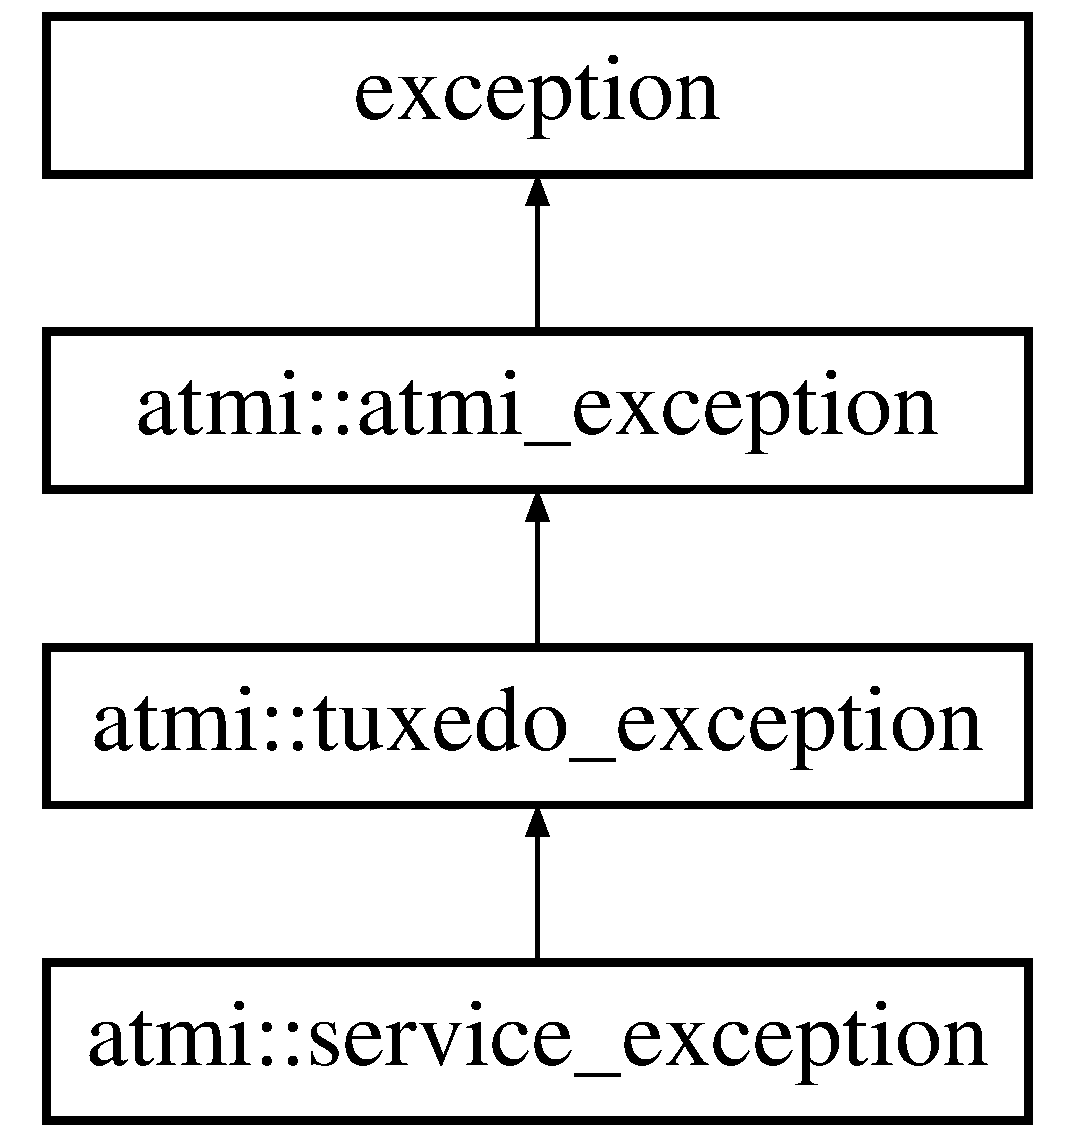
\includegraphics[height=4.000000cm]{classatmi_1_1service__exception}
\end{center}
\end{figure}
\subsection*{Public Member Functions}
\begin{DoxyCompactItemize}
\item 
{\footnotesize template$<$typename... Args$>$ }\\\hyperlink{classatmi_1_1service__exception_aaaf22082b56169c161573ec3dfd4a6fd}{service\+\_\+exception} (const char $\ast$msg, const Args \&...args)
\end{DoxyCompactItemize}
\subsection*{Additional Inherited Members}


\subsection{Detailed Description}
Thrown when a T\+P\+E\+S\+V\+C\+E\+R\+R s returned after a T\+P call. 

\subsection{Constructor \& Destructor Documentation}
\hypertarget{classatmi_1_1service__exception_aaaf22082b56169c161573ec3dfd4a6fd}{\index{atmi\+::service\+\_\+exception@{atmi\+::service\+\_\+exception}!service\+\_\+exception@{service\+\_\+exception}}
\index{service\+\_\+exception@{service\+\_\+exception}!atmi\+::service\+\_\+exception@{atmi\+::service\+\_\+exception}}
\subsubsection[{service\+\_\+exception}]{\setlength{\rightskip}{0pt plus 5cm}template$<$typename... Args$>$ atmi\+::service\+\_\+exception\+::service\+\_\+exception (
\begin{DoxyParamCaption}
\item[{const char $\ast$}]{msg, }
\item[{const Args \&...}]{args}
\end{DoxyParamCaption}
)\hspace{0.3cm}{\ttfamily [inline]}}}\label{classatmi_1_1service__exception_aaaf22082b56169c161573ec3dfd4a6fd}
new instance.


\begin{DoxyParams}{Parameters}
{\em msg} & error message \\
\hline
{\em args} & error message parameters (variadic). \\
\hline
\end{DoxyParams}


The documentation for this class was generated from the following file\+:\begin{DoxyCompactItemize}
\item 
include/atmi/exceptions.\+hpp\end{DoxyCompactItemize}

\hypertarget{classatmi_1_1_tfield}{\section{atmi\+:\+:Tfield$<$ T $>$ Class Template Reference}
\label{classatmi_1_1_tfield}\index{atmi\+::\+Tfield$<$ T $>$@{atmi\+::\+Tfield$<$ T $>$}}
}


 




{\ttfamily \#include $<$fields.\+hpp$>$}

Inheritance diagram for atmi\+:\+:Tfield$<$ T $>$\+:\begin{figure}[H]
\begin{center}
\leavevmode
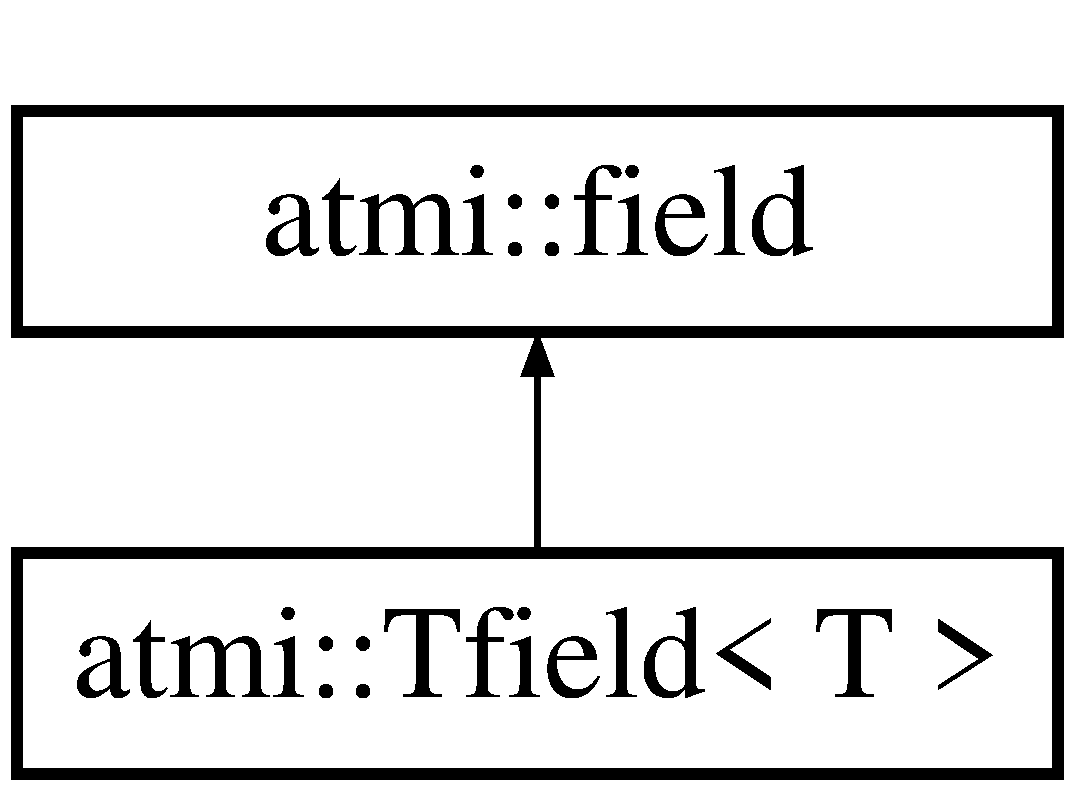
\includegraphics[height=2.000000cm]{classatmi_1_1_tfield}
\end{center}
\end{figure}
\subsection*{Public Member Functions}
\begin{DoxyCompactItemize}
\item 
\hyperlink{classatmi_1_1_tfield_a533be0f49416e622563e7f437e7e9014}{Tfield} ()
\item 
\hyperlink{classatmi_1_1_tfield_a10739dd7cef7fad99e5c32213bc69fca}{Tfield} (F\+L\+D\+I\+D32 field\+\_\+id)
\item 
\hyperlink{classatmi_1_1_tfield_a9718a2fcffa95fda6e31f18815d05dbe}{Tfield} (const char $\ast$\hyperlink{classatmi_1_1field_a0fbc5a958a0af8286e339b088ee69bc8}{name})
\item 
virtual void \hyperlink{classatmi_1_1_tfield_ac458fcdcce36a34d8beed526ca1e385a}{set\+\_\+id} (F\+L\+D\+I\+D32 field\+\_\+id)
\item 
virtual F\+L\+D\+L\+E\+N32 \hyperlink{classatmi_1_1_tfield_a6138c508841c4a837ea8c8e089755278}{length} ()
\item 
T \hyperlink{classatmi_1_1_tfield_a7903e881d35805b1477b1ef8f2928f4e}{operator=} (T v)
\item 
\hyperlink{classatmi_1_1_tfield_ad8b13cf9dc43ad4a896ab96a1aefb31f}{operator T} ()
\end{DoxyCompactItemize}
\subsection*{Protected Member Functions}
\begin{DoxyCompactItemize}
\item 
virtual int \hyperlink{classatmi_1_1_tfield_a7bd1997e976116990ad0e2072320db77}{set} (\hyperlink{classatmi_1_1buffer}{buffer} \&b)
\item 
virtual int \hyperlink{classatmi_1_1_tfield_a4962b3aa080aba4ecffc7f3fa98be2da}{add} (\hyperlink{classatmi_1_1buffer}{buffer} \&b)
\item 
virtual int \hyperlink{classatmi_1_1_tfield_aa70ce8893913c8f3d968cae72f2cdd11}{get} (\hyperlink{classatmi_1_1buffer}{buffer} \&b)
\item 
virtual int \hyperlink{classatmi_1_1_tfield_ae8de2dd360d04fc2465e4169b239c222}{get} (\hyperlink{classatmi_1_1buffer}{buffer} \&b, F\+L\+D\+O\+C\+C32 occ)
\end{DoxyCompactItemize}
\subsection*{Protected Attributes}
\begin{DoxyCompactItemize}
\item 
\hypertarget{classatmi_1_1_tfield_a89852f63b07d2f6d27d9866b030d1c5d}{T \hyperlink{classatmi_1_1_tfield_a89852f63b07d2f6d27d9866b030d1c5d}{value}}\label{classatmi_1_1_tfield_a89852f63b07d2f6d27d9866b030d1c5d}

\begin{DoxyCompactList}\small\item\em field's current value \end{DoxyCompactList}\end{DoxyCompactItemize}


\subsection{Detailed Description}
\subsubsection*{template$<$class T$>$class atmi\+::\+Tfield$<$ T $>$}



Template that handles short, long, char, double data type.

When a new instance is created, occurence is set to 0 making it possible to set values withour a prior call to add. 

\subsection{Constructor \& Destructor Documentation}
\hypertarget{classatmi_1_1_tfield_a533be0f49416e622563e7f437e7e9014}{\index{atmi\+::\+Tfield@{atmi\+::\+Tfield}!Tfield@{Tfield}}
\index{Tfield@{Tfield}!atmi\+::\+Tfield@{atmi\+::\+Tfield}}
\subsubsection[{Tfield}]{\setlength{\rightskip}{0pt plus 5cm}template$<$class T $>$ {\bf atmi\+::\+Tfield}$<$ T $>$\+::{\bf Tfield} (
\begin{DoxyParamCaption}
{}
\end{DoxyParamCaption}
)\hspace{0.3cm}{\ttfamily [inline]}}}\label{classatmi_1_1_tfield_a533be0f49416e622563e7f437e7e9014}
default constructor.

The instance cannot be used until set\+\_\+field\+\_\+id is successfully called.

\begin{DoxySince}{Since}
v4.\+2.\+0 
\end{DoxySince}
\hypertarget{classatmi_1_1_tfield_a10739dd7cef7fad99e5c32213bc69fca}{\index{atmi\+::\+Tfield@{atmi\+::\+Tfield}!Tfield@{Tfield}}
\index{Tfield@{Tfield}!atmi\+::\+Tfield@{atmi\+::\+Tfield}}
\subsubsection[{Tfield}]{\setlength{\rightskip}{0pt plus 5cm}template$<$class T $>$ {\bf atmi\+::\+Tfield}$<$ T $>$\+::{\bf Tfield} (
\begin{DoxyParamCaption}
\item[{F\+L\+D\+I\+D32}]{field\+\_\+id}
\end{DoxyParamCaption}
)\hspace{0.3cm}{\ttfamily [inline]}, {\ttfamily [explicit]}}}\label{classatmi_1_1_tfield_a10739dd7cef7fad99e5c32213bc69fca}
Constructs a \hyperlink{classatmi_1_1_tfield}{Tfield} for the passed field id

The search is done in the tables identified by F\+L\+D\+T\+B\+L\+D\+I\+R32 and F\+I\+E\+L\+D\+T\+B\+L\+S32


\begin{DoxyParams}{Parameters}
{\em field\+\_\+id} & the fml field id to setup (as defined in the F\+M\+L tables) \\
\hline
\end{DoxyParams}
\hypertarget{classatmi_1_1_tfield_a9718a2fcffa95fda6e31f18815d05dbe}{\index{atmi\+::\+Tfield@{atmi\+::\+Tfield}!Tfield@{Tfield}}
\index{Tfield@{Tfield}!atmi\+::\+Tfield@{atmi\+::\+Tfield}}
\subsubsection[{Tfield}]{\setlength{\rightskip}{0pt plus 5cm}template$<$class T $>$ {\bf atmi\+::\+Tfield}$<$ T $>$\+::{\bf Tfield} (
\begin{DoxyParamCaption}
\item[{const char $\ast$}]{name}
\end{DoxyParamCaption}
)\hspace{0.3cm}{\ttfamily [inline]}, {\ttfamily [explicit]}}}\label{classatmi_1_1_tfield_a9718a2fcffa95fda6e31f18815d05dbe}
Constructs a \hyperlink{classatmi_1_1_tfield}{Tfield} for the passed name

The search is done in the tables identified by F\+L\+D\+T\+B\+L\+D\+I\+R32 and F\+I\+E\+L\+D\+T\+B\+L\+S32


\begin{DoxyParams}{Parameters}
{\em name} & the fml field name to setup (as defined in the F\+M\+L tables) \\
\hline
\end{DoxyParams}


\subsection{Member Function Documentation}
\hypertarget{classatmi_1_1_tfield_a4962b3aa080aba4ecffc7f3fa98be2da}{\index{atmi\+::\+Tfield@{atmi\+::\+Tfield}!add@{add}}
\index{add@{add}!atmi\+::\+Tfield@{atmi\+::\+Tfield}}
\subsubsection[{add}]{\setlength{\rightskip}{0pt plus 5cm}template$<$class T $>$ virtual int {\bf atmi\+::\+Tfield}$<$ T $>$\+::add (
\begin{DoxyParamCaption}
\item[{{\bf buffer} \&}]{b}
\end{DoxyParamCaption}
)\hspace{0.3cm}{\ttfamily [inline]}, {\ttfamily [protected]}, {\ttfamily [virtual]}}}\label{classatmi_1_1_tfield_a4962b3aa080aba4ecffc7f3fa98be2da}
add the fiels into the buffer

When successfull the value of occurence is se


\begin{DoxyParams}{Parameters}
{\em b} & buffer in which to add the field. \\
\hline
\end{DoxyParams}
\begin{DoxySeeAlso}{See also}
\hyperlink{classatmi_1_1field_a161b9b7037c49fbcf86518fcb35e779c}{occurence} 
\end{DoxySeeAlso}


Implements \hyperlink{classatmi_1_1field_a5441bc87ba4bc3e9eb37c6db6a29688f}{atmi\+::field}.

\hypertarget{classatmi_1_1_tfield_aa70ce8893913c8f3d968cae72f2cdd11}{\index{atmi\+::\+Tfield@{atmi\+::\+Tfield}!get@{get}}
\index{get@{get}!atmi\+::\+Tfield@{atmi\+::\+Tfield}}
\subsubsection[{get}]{\setlength{\rightskip}{0pt plus 5cm}template$<$class T $>$ virtual int {\bf atmi\+::\+Tfield}$<$ T $>$\+::get (
\begin{DoxyParamCaption}
\item[{{\bf buffer} \&}]{b}
\end{DoxyParamCaption}
)\hspace{0.3cm}{\ttfamily [inline]}, {\ttfamily [protected]}, {\ttfamily [virtual]}}}\label{classatmi_1_1_tfield_aa70ce8893913c8f3d968cae72f2cdd11}
Retrieves the value of the field found into the buffer.


\begin{DoxyParams}{Parameters}
{\em b} & buffer from which to retrieve the field's value \\
\hline
\end{DoxyParams}


Implements \hyperlink{classatmi_1_1field_aae2d3df756e816b5db8f729039a59a51}{atmi\+::field}.

\hypertarget{classatmi_1_1_tfield_ae8de2dd360d04fc2465e4169b239c222}{\index{atmi\+::\+Tfield@{atmi\+::\+Tfield}!get@{get}}
\index{get@{get}!atmi\+::\+Tfield@{atmi\+::\+Tfield}}
\subsubsection[{get}]{\setlength{\rightskip}{0pt plus 5cm}template$<$class T $>$ virtual int {\bf atmi\+::\+Tfield}$<$ T $>$\+::get (
\begin{DoxyParamCaption}
\item[{{\bf buffer} \&}]{b, }
\item[{F\+L\+D\+O\+C\+C32}]{occ}
\end{DoxyParamCaption}
)\hspace{0.3cm}{\ttfamily [inline]}, {\ttfamily [protected]}, {\ttfamily [virtual]}}}\label{classatmi_1_1_tfield_ae8de2dd360d04fc2465e4169b239c222}
Retrieves the value of the field's occurence found into the buffer

Upon success the value of occurence is set to the retrieved occurence.


\begin{DoxyParams}{Parameters}
{\em b} & buffer from which to retrieve the field's value \\
\hline
{\em occ} & occurence to retreive \\
\hline
\end{DoxyParams}
\begin{DoxySeeAlso}{See also}
\hyperlink{classatmi_1_1field_a161b9b7037c49fbcf86518fcb35e779c}{occurence} 
\end{DoxySeeAlso}


Implements \hyperlink{classatmi_1_1field_a56ce53fabe290b94463f87936515ec46}{atmi\+::field}.

\hypertarget{classatmi_1_1_tfield_a6138c508841c4a837ea8c8e089755278}{\index{atmi\+::\+Tfield@{atmi\+::\+Tfield}!length@{length}}
\index{length@{length}!atmi\+::\+Tfield@{atmi\+::\+Tfield}}
\subsubsection[{length}]{\setlength{\rightskip}{0pt plus 5cm}template$<$class T $>$ virtual F\+L\+D\+L\+E\+N32 {\bf atmi\+::\+Tfield}$<$ T $>$\+::length (
\begin{DoxyParamCaption}
{}
\end{DoxyParamCaption}
)\hspace{0.3cm}{\ttfamily [inline]}, {\ttfamily [virtual]}}}\label{classatmi_1_1_tfield_a6138c508841c4a837ea8c8e089755278}
\begin{DoxyReturn}{Returns}
de length (or size) of the field's data 
\end{DoxyReturn}


Implements \hyperlink{classatmi_1_1field_a296771293135085d91aa9aefd108d44d}{atmi\+::field}.

\hypertarget{classatmi_1_1_tfield_ad8b13cf9dc43ad4a896ab96a1aefb31f}{\index{atmi\+::\+Tfield@{atmi\+::\+Tfield}!operator T@{operator T}}
\index{operator T@{operator T}!atmi\+::\+Tfield@{atmi\+::\+Tfield}}
\subsubsection[{operator T}]{\setlength{\rightskip}{0pt plus 5cm}template$<$class T $>$ {\bf atmi\+::\+Tfield}$<$ T $>$\+::operator T (
\begin{DoxyParamCaption}
{}
\end{DoxyParamCaption}
)\hspace{0.3cm}{\ttfamily [inline]}}}\label{classatmi_1_1_tfield_ad8b13cf9dc43ad4a896ab96a1aefb31f}
casts the field value ... Tfield$<$int$>$ f (fid); f = 156 ; int x = f ; // returns 156 ... \hypertarget{classatmi_1_1_tfield_a7903e881d35805b1477b1ef8f2928f4e}{\index{atmi\+::\+Tfield@{atmi\+::\+Tfield}!operator=@{operator=}}
\index{operator=@{operator=}!atmi\+::\+Tfield@{atmi\+::\+Tfield}}
\subsubsection[{operator=}]{\setlength{\rightskip}{0pt plus 5cm}template$<$class T $>$ T {\bf atmi\+::\+Tfield}$<$ T $>$\+::operator= (
\begin{DoxyParamCaption}
\item[{T}]{v}
\end{DoxyParamCaption}
)\hspace{0.3cm}{\ttfamily [inline]}}}\label{classatmi_1_1_tfield_a7903e881d35805b1477b1ef8f2928f4e}
Assigns a value to the field ... Tfield$<$int$>$ f (fid); f = 156 ; // Set value to 156 ... \hypertarget{classatmi_1_1_tfield_a7bd1997e976116990ad0e2072320db77}{\index{atmi\+::\+Tfield@{atmi\+::\+Tfield}!set@{set}}
\index{set@{set}!atmi\+::\+Tfield@{atmi\+::\+Tfield}}
\subsubsection[{set}]{\setlength{\rightskip}{0pt plus 5cm}template$<$class T $>$ virtual int {\bf atmi\+::\+Tfield}$<$ T $>$\+::set (
\begin{DoxyParamCaption}
\item[{{\bf buffer} \&}]{b}
\end{DoxyParamCaption}
)\hspace{0.3cm}{\ttfamily [inline]}, {\ttfamily [protected]}, {\ttfamily [virtual]}}}\label{classatmi_1_1_tfield_a7bd1997e976116990ad0e2072320db77}
set the value of the field's value


\begin{DoxyParams}{Parameters}
{\em b} & the buffer in which the value must be changed \\
\hline
\end{DoxyParams}


Implements \hyperlink{classatmi_1_1field_a41bb209965d627d2e67c839bece5372c}{atmi\+::field}.

\hypertarget{classatmi_1_1_tfield_ac458fcdcce36a34d8beed526ca1e385a}{\index{atmi\+::\+Tfield@{atmi\+::\+Tfield}!set\+\_\+id@{set\+\_\+id}}
\index{set\+\_\+id@{set\+\_\+id}!atmi\+::\+Tfield@{atmi\+::\+Tfield}}
\subsubsection[{set\+\_\+id}]{\setlength{\rightskip}{0pt plus 5cm}template$<$class T $>$ virtual void {\bf atmi\+::\+Tfield}$<$ T $>$\+::set\+\_\+id (
\begin{DoxyParamCaption}
\item[{F\+L\+D\+I\+D32}]{field\+\_\+id}
\end{DoxyParamCaption}
)\hspace{0.3cm}{\ttfamily [inline]}, {\ttfamily [virtual]}}}\label{classatmi_1_1_tfield_ac458fcdcce36a34d8beed526ca1e385a}
set field id.

This template only handles numerical field I\+Ds.


\begin{DoxyParams}{Parameters}
{\em field\+\_\+id} & the fml field id to setup (as defined in the F\+M\+L tables) \\
\hline
\end{DoxyParams}
This array is used to check that F\+M\+L type matches template \hyperlink{classatmi_1_1_tfield}{Tfield}'s type 

Reimplemented from \hyperlink{classatmi_1_1field_a1d95c3b0f4ae491037ef51b8586a0083}{atmi\+::field}.



The documentation for this class was generated from the following file\+:\begin{DoxyCompactItemize}
\item 
include/atmi/fields.\+hpp\end{DoxyCompactItemize}

\hypertarget{classatmi_1_1_tfield_3_01char_01_5_01_4}{\section{atmi\+:\+:Tfield$<$ char $\ast$ $>$ Class Template Reference}
\label{classatmi_1_1_tfield_3_01char_01_5_01_4}\index{atmi\+::\+Tfield$<$ char $\ast$ $>$@{atmi\+::\+Tfield$<$ char $\ast$ $>$}}
}


 




{\ttfamily \#include $<$carray\+\_\+field.\+hpp$>$}

Inheritance diagram for atmi\+:\+:Tfield$<$ char $\ast$ $>$\+:\begin{figure}[H]
\begin{center}
\leavevmode
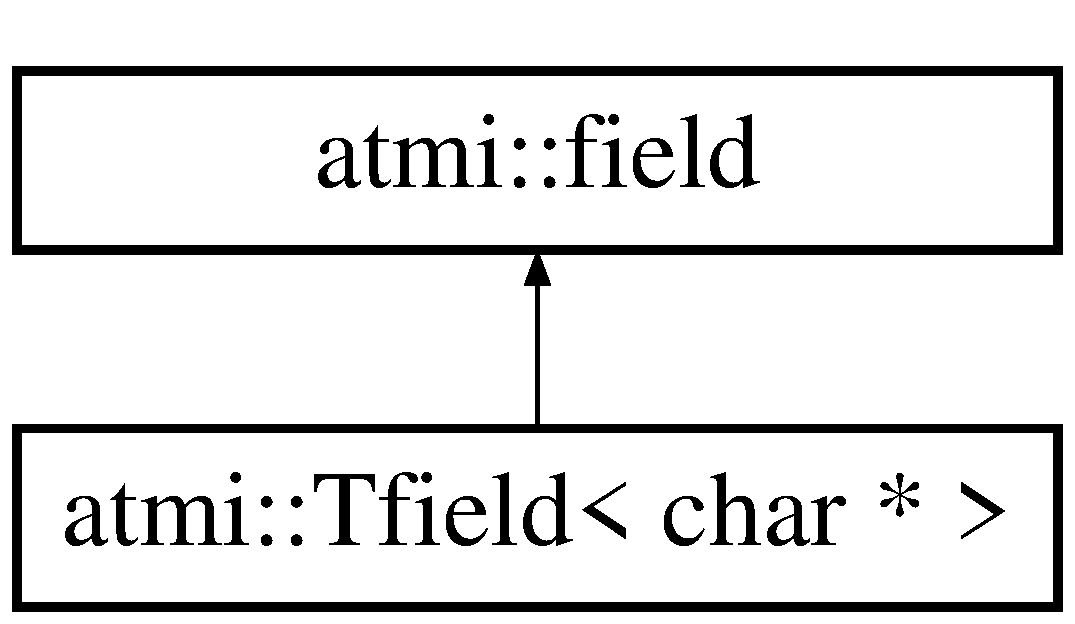
\includegraphics[height=2.000000cm]{classatmi_1_1_tfield_3_01char_01_5_01_4}
\end{center}
\end{figure}
\subsection*{Public Member Functions}
\begin{DoxyCompactItemize}
\item 
\hyperlink{classatmi_1_1_tfield_3_01char_01_5_01_4_ad16891d15a65e85408962ec962e57bd8}{Tfield} (F\+L\+D\+I\+D32 fid)
\item 
\hyperlink{classatmi_1_1_tfield_3_01char_01_5_01_4_a197bf4f86d8053adcf8afdcd839b85cc}{Tfield} (const char $\ast$n)
\item 
F\+L\+D\+L\+E\+N32 \hyperlink{classatmi_1_1_tfield_3_01char_01_5_01_4_a4dbdcf1e58232003aa20bb991f49f2f4}{buffer\+\_\+size} () const 
\item 
virtual F\+L\+D\+L\+E\+N32 \hyperlink{classatmi_1_1_tfield_3_01char_01_5_01_4_aa97dec8559724186b62997409f04bf3f}{length} ()
\item 
void \hyperlink{classatmi_1_1_tfield_3_01char_01_5_01_4_aa716c65e01963069f2abbe0ffee894f3}{set\+\_\+char\+\_\+array} (const char $\ast$\hyperlink{group__fml_ga8b57f9a4e2453d8e5d82ac0016e35e87}{carray}, F\+L\+D\+L\+E\+N32 size)
\item 
virtual void \hyperlink{classatmi_1_1_tfield_3_01char_01_5_01_4_a009218c6eec4478fb0e0a4c2741df5c2}{get\+\_\+char\+\_\+array} (char $\ast$\hyperlink{group__fml_ga8b57f9a4e2453d8e5d82ac0016e35e87}{carray}, F\+L\+D\+L\+E\+N32 size)
\item 
\hyperlink{classatmi_1_1_tfield}{Tfield}$<$ char $\ast$ $>$ \& \hyperlink{classatmi_1_1_tfield_3_01char_01_5_01_4_a486559e383ca6ae8002cb527901b716f}{operator=} (\hyperlink{classatmi_1_1_tfield}{Tfield}$<$ char $\ast$ $>$ \&\hyperlink{group__fml_ga8b57f9a4e2453d8e5d82ac0016e35e87}{carray})
\item 
void \hyperlink{classatmi_1_1_tfield_3_01char_01_5_01_4_a3bc71ae4ac7ae39aa21dd6533c230fda}{free\+\_\+ressources} ()
\item 
char \& \hyperlink{classatmi_1_1_tfield_3_01char_01_5_01_4_a0d4241c582c4e0af4e55ea6dfcf8ae8b}{operator\mbox{[}$\,$\mbox{]}} (int index)
\end{DoxyCompactItemize}
\subsection*{Protected Member Functions}
\begin{DoxyCompactItemize}
\item 
virtual int \hyperlink{classatmi_1_1_tfield_3_01char_01_5_01_4_af7be84fbdff0665d9c94b83872b299b7}{set} (\hyperlink{classatmi_1_1buffer}{buffer} \&b)
\item 
virtual int \hyperlink{classatmi_1_1_tfield_3_01char_01_5_01_4_ae3036c038b361aee2fc357c1c7d1304a}{add} (\hyperlink{classatmi_1_1buffer}{buffer} \&b)
\item 
virtual int \hyperlink{classatmi_1_1_tfield_3_01char_01_5_01_4_a5df77c9bee99916f6d14f5beeec54dac}{get} (\hyperlink{classatmi_1_1buffer}{buffer} \&b)
\item 
virtual int \hyperlink{classatmi_1_1_tfield_3_01char_01_5_01_4_afaedd7d5902233652bed642bdceb9db1}{get} (\hyperlink{classatmi_1_1buffer}{buffer} \&b, F\+L\+D\+O\+C\+C32 occ)
\begin{DoxyCompactList}\small\item\em int get ( buffer \&b ) \end{DoxyCompactList}\end{DoxyCompactItemize}
\subsection*{Protected Attributes}
\begin{DoxyCompactItemize}
\item 
\hypertarget{classatmi_1_1_tfield_3_01char_01_5_01_4_aa25bb2aa5ab92371fb9b68f0659ced31}{F\+L\+D\+L\+E\+N32 \hyperlink{classatmi_1_1_tfield_3_01char_01_5_01_4_aa25bb2aa5ab92371fb9b68f0659ced31}{\+\_\+length}}\label{classatmi_1_1_tfield_3_01char_01_5_01_4_aa25bb2aa5ab92371fb9b68f0659ced31}

\begin{DoxyCompactList}\small\item\em field length (bytes) \end{DoxyCompactList}\item 
\hypertarget{classatmi_1_1_tfield_3_01char_01_5_01_4_a5e7218b977e644a60ed6fbb5d1957e75}{F\+L\+D\+L\+E\+N32 \hyperlink{classatmi_1_1_tfield_3_01char_01_5_01_4_a5e7218b977e644a60ed6fbb5d1957e75}{\+\_\+buffer\+\_\+size}}\label{classatmi_1_1_tfield_3_01char_01_5_01_4_a5e7218b977e644a60ed6fbb5d1957e75}

\begin{DoxyCompactList}\small\item\em back end size(bytes) \end{DoxyCompactList}\item 
\hypertarget{classatmi_1_1_tfield_3_01char_01_5_01_4_a425204246b56c8e10459b53b563800c9}{char $\ast$ \hyperlink{classatmi_1_1_tfield_3_01char_01_5_01_4_a425204246b56c8e10459b53b563800c9}{\+\_\+value}}\label{classatmi_1_1_tfield_3_01char_01_5_01_4_a425204246b56c8e10459b53b563800c9}

\begin{DoxyCompactList}\small\item\em chacater buffer \end{DoxyCompactList}\end{DoxyCompactItemize}


\subsection{Detailed Description}
\subsubsection*{template$<$$>$class atmi\+::\+Tfield$<$ char $\ast$ $>$}



Specialization of template \hyperlink{classatmi_1_1_tfield}{Tfield} which handles C\+A\+R\+R\+A\+Y typed fields.

This class is using a std\+::string object to hold and handle char $\ast$ data When a new instance is created, occurence is set to 0 making it possible to set values withour a prior call to add. 

\subsection{Constructor \& Destructor Documentation}
\hypertarget{classatmi_1_1_tfield_3_01char_01_5_01_4_ad16891d15a65e85408962ec962e57bd8}{\index{atmi\+::\+Tfield$<$ char $\ast$ $>$@{atmi\+::\+Tfield$<$ char $\ast$ $>$}!Tfield@{Tfield}}
\index{Tfield@{Tfield}!atmi\+::\+Tfield$<$ char $\ast$ $>$@{atmi\+::\+Tfield$<$ char $\ast$ $>$}}
\subsubsection[{Tfield}]{\setlength{\rightskip}{0pt plus 5cm}{\bf atmi\+::\+Tfield}$<$ char $\ast$ $>$\+::{\bf Tfield} (
\begin{DoxyParamCaption}
\item[{F\+L\+D\+I\+D32}]{fid}
\end{DoxyParamCaption}
)\hspace{0.3cm}{\ttfamily [inline]}, {\ttfamily [explicit]}}}\label{classatmi_1_1_tfield_3_01char_01_5_01_4_ad16891d15a65e85408962ec962e57bd8}
Constructs a \hyperlink{classatmi_1_1_tfield}{Tfield} for the passed field id

The search is done in the tables identified by F\+L\+D\+T\+B\+L\+D\+I\+R32 and F\+I\+E\+L\+D\+T\+B\+L\+S32


\begin{DoxyParams}{Parameters}
{\em fid} & the fml field id to setup (as defined in the F\+M\+L tables) \\
\hline
\end{DoxyParams}
\hypertarget{classatmi_1_1_tfield_3_01char_01_5_01_4_a197bf4f86d8053adcf8afdcd839b85cc}{\index{atmi\+::\+Tfield$<$ char $\ast$ $>$@{atmi\+::\+Tfield$<$ char $\ast$ $>$}!Tfield@{Tfield}}
\index{Tfield@{Tfield}!atmi\+::\+Tfield$<$ char $\ast$ $>$@{atmi\+::\+Tfield$<$ char $\ast$ $>$}}
\subsubsection[{Tfield}]{\setlength{\rightskip}{0pt plus 5cm}{\bf atmi\+::\+Tfield}$<$ char $\ast$ $>$\+::{\bf Tfield} (
\begin{DoxyParamCaption}
\item[{const char $\ast$}]{n}
\end{DoxyParamCaption}
)\hspace{0.3cm}{\ttfamily [inline]}, {\ttfamily [explicit]}}}\label{classatmi_1_1_tfield_3_01char_01_5_01_4_a197bf4f86d8053adcf8afdcd839b85cc}
Constructs a \hyperlink{classatmi_1_1_tfield}{Tfield} for the passed name

The search is done in the tables identified by F\+L\+D\+T\+B\+L\+D\+I\+R32 and F\+I\+E\+L\+D\+T\+B\+L\+S32


\begin{DoxyParams}{Parameters}
{\em n} & the fml field name to setup (as defined in the F\+M\+L tables) \\
\hline
\end{DoxyParams}


\subsection{Member Function Documentation}
\hypertarget{classatmi_1_1_tfield_3_01char_01_5_01_4_ae3036c038b361aee2fc357c1c7d1304a}{\index{atmi\+::\+Tfield$<$ char $\ast$ $>$@{atmi\+::\+Tfield$<$ char $\ast$ $>$}!add@{add}}
\index{add@{add}!atmi\+::\+Tfield$<$ char $\ast$ $>$@{atmi\+::\+Tfield$<$ char $\ast$ $>$}}
\subsubsection[{add}]{\setlength{\rightskip}{0pt plus 5cm}virtual int {\bf atmi\+::\+Tfield}$<$ char $\ast$ $>$\+::add (
\begin{DoxyParamCaption}
\item[{{\bf buffer} \&}]{b}
\end{DoxyParamCaption}
)\hspace{0.3cm}{\ttfamily [inline]}, {\ttfamily [protected]}, {\ttfamily [virtual]}}}\label{classatmi_1_1_tfield_3_01char_01_5_01_4_ae3036c038b361aee2fc357c1c7d1304a}
implement a Fadd32 call for carrays


\begin{DoxyParams}{Parameters}
{\em b} & buffer to apply the change in \\
\hline
\end{DoxyParams}


Implements \hyperlink{classatmi_1_1field_a5441bc87ba4bc3e9eb37c6db6a29688f}{atmi\+::field}.

\hypertarget{classatmi_1_1_tfield_3_01char_01_5_01_4_a4dbdcf1e58232003aa20bb991f49f2f4}{\index{atmi\+::\+Tfield$<$ char $\ast$ $>$@{atmi\+::\+Tfield$<$ char $\ast$ $>$}!buffer\+\_\+size@{buffer\+\_\+size}}
\index{buffer\+\_\+size@{buffer\+\_\+size}!atmi\+::\+Tfield$<$ char $\ast$ $>$@{atmi\+::\+Tfield$<$ char $\ast$ $>$}}
\subsubsection[{buffer\+\_\+size}]{\setlength{\rightskip}{0pt plus 5cm}F\+L\+D\+L\+E\+N32 {\bf atmi\+::\+Tfield}$<$ char $\ast$ $>$\+::buffer\+\_\+size (
\begin{DoxyParamCaption}
{}
\end{DoxyParamCaption}
) const\hspace{0.3cm}{\ttfamily [inline]}}}\label{classatmi_1_1_tfield_3_01char_01_5_01_4_a4dbdcf1e58232003aa20bb991f49f2f4}
\begin{DoxyReturn}{Returns}
backend allocation 
\end{DoxyReturn}
\hypertarget{classatmi_1_1_tfield_3_01char_01_5_01_4_a3bc71ae4ac7ae39aa21dd6533c230fda}{\index{atmi\+::\+Tfield$<$ char $\ast$ $>$@{atmi\+::\+Tfield$<$ char $\ast$ $>$}!free\+\_\+ressources@{free\+\_\+ressources}}
\index{free\+\_\+ressources@{free\+\_\+ressources}!atmi\+::\+Tfield$<$ char $\ast$ $>$@{atmi\+::\+Tfield$<$ char $\ast$ $>$}}
\subsubsection[{free\+\_\+ressources}]{\setlength{\rightskip}{0pt plus 5cm}void {\bf atmi\+::\+Tfield}$<$ char $\ast$ $>$\+::free\+\_\+ressources (
\begin{DoxyParamCaption}
{}
\end{DoxyParamCaption}
)\hspace{0.3cm}{\ttfamily [inline]}}}\label{classatmi_1_1_tfield_3_01char_01_5_01_4_a3bc71ae4ac7ae39aa21dd6533c230fda}
de-\/allocate internal ressources (mainly the caray). \hypertarget{classatmi_1_1_tfield_3_01char_01_5_01_4_a5df77c9bee99916f6d14f5beeec54dac}{\index{atmi\+::\+Tfield$<$ char $\ast$ $>$@{atmi\+::\+Tfield$<$ char $\ast$ $>$}!get@{get}}
\index{get@{get}!atmi\+::\+Tfield$<$ char $\ast$ $>$@{atmi\+::\+Tfield$<$ char $\ast$ $>$}}
\subsubsection[{get}]{\setlength{\rightskip}{0pt plus 5cm}virtual int {\bf atmi\+::\+Tfield}$<$ char $\ast$ $>$\+::get (
\begin{DoxyParamCaption}
\item[{{\bf buffer} \&}]{b}
\end{DoxyParamCaption}
)\hspace{0.3cm}{\ttfamily [inline]}, {\ttfamily [protected]}, {\ttfamily [virtual]}}}\label{classatmi_1_1_tfield_3_01char_01_5_01_4_a5df77c9bee99916f6d14f5beeec54dac}
retreive the current carray content.

the content is copied into character array (backend). if the backend is too small a bigger one is allocated and used.


\begin{DoxyParams}{Parameters}
{\em b} & buffer to apply the change in \\
\hline
\end{DoxyParams}


Implements \hyperlink{classatmi_1_1field_aae2d3df756e816b5db8f729039a59a51}{atmi\+::field}.

\hypertarget{classatmi_1_1_tfield_3_01char_01_5_01_4_afaedd7d5902233652bed642bdceb9db1}{\index{atmi\+::\+Tfield$<$ char $\ast$ $>$@{atmi\+::\+Tfield$<$ char $\ast$ $>$}!get@{get}}
\index{get@{get}!atmi\+::\+Tfield$<$ char $\ast$ $>$@{atmi\+::\+Tfield$<$ char $\ast$ $>$}}
\subsubsection[{get}]{\setlength{\rightskip}{0pt plus 5cm}virtual int {\bf atmi\+::\+Tfield}$<$ char $\ast$ $>$\+::get (
\begin{DoxyParamCaption}
\item[{{\bf buffer} \&}]{b, }
\item[{F\+L\+D\+O\+C\+C32}]{occ}
\end{DoxyParamCaption}
)\hspace{0.3cm}{\ttfamily [inline]}, {\ttfamily [protected]}, {\ttfamily [virtual]}}}\label{classatmi_1_1_tfield_3_01char_01_5_01_4_afaedd7d5902233652bed642bdceb9db1}


int get ( buffer \&b ) 

int get ( buffer \&b )


\begin{DoxyParams}{Parameters}
{\em b} & fielded buffer \\
\hline
{\em occ} & field occurence to search for \\
\hline
\end{DoxyParams}


Implements \hyperlink{classatmi_1_1field_a56ce53fabe290b94463f87936515ec46}{atmi\+::field}.

\hypertarget{classatmi_1_1_tfield_3_01char_01_5_01_4_a009218c6eec4478fb0e0a4c2741df5c2}{\index{atmi\+::\+Tfield$<$ char $\ast$ $>$@{atmi\+::\+Tfield$<$ char $\ast$ $>$}!get\+\_\+char\+\_\+array@{get\+\_\+char\+\_\+array}}
\index{get\+\_\+char\+\_\+array@{get\+\_\+char\+\_\+array}!atmi\+::\+Tfield$<$ char $\ast$ $>$@{atmi\+::\+Tfield$<$ char $\ast$ $>$}}
\subsubsection[{get\+\_\+char\+\_\+array}]{\setlength{\rightskip}{0pt plus 5cm}virtual void {\bf atmi\+::\+Tfield}$<$ char $\ast$ $>$\+::get\+\_\+char\+\_\+array (
\begin{DoxyParamCaption}
\item[{char $\ast$}]{carray, }
\item[{F\+L\+D\+L\+E\+N32}]{size}
\end{DoxyParamCaption}
)\hspace{0.3cm}{\ttfamily [inline]}, {\ttfamily [virtual]}}}\label{classatmi_1_1_tfield_3_01char_01_5_01_4_a009218c6eec4478fb0e0a4c2741df5c2}
copy (memcpy) the field's value into carray.

if the given size is smaller than the actual field size, then size characters are copied into your buffer. If size is bigger than the actual field size, then field length characters are copied meaning your data will be truncated.


\begin{DoxyParams}{Parameters}
{\em carray} & pointer to a previously allocted character buffer \\
\hline
{\em size} & character buffer size \\
\hline
\end{DoxyParams}
\hypertarget{classatmi_1_1_tfield_3_01char_01_5_01_4_aa97dec8559724186b62997409f04bf3f}{\index{atmi\+::\+Tfield$<$ char $\ast$ $>$@{atmi\+::\+Tfield$<$ char $\ast$ $>$}!length@{length}}
\index{length@{length}!atmi\+::\+Tfield$<$ char $\ast$ $>$@{atmi\+::\+Tfield$<$ char $\ast$ $>$}}
\subsubsection[{length}]{\setlength{\rightskip}{0pt plus 5cm}virtual F\+L\+D\+L\+E\+N32 {\bf atmi\+::\+Tfield}$<$ char $\ast$ $>$\+::length (
\begin{DoxyParamCaption}
{}
\end{DoxyParamCaption}
)\hspace{0.3cm}{\ttfamily [inline]}, {\ttfamily [virtual]}}}\label{classatmi_1_1_tfield_3_01char_01_5_01_4_aa97dec8559724186b62997409f04bf3f}
\begin{DoxyReturn}{Returns}
returns the size of the carray 
\end{DoxyReturn}


Implements \hyperlink{classatmi_1_1field_a296771293135085d91aa9aefd108d44d}{atmi\+::field}.

\hypertarget{classatmi_1_1_tfield_3_01char_01_5_01_4_a486559e383ca6ae8002cb527901b716f}{\index{atmi\+::\+Tfield$<$ char $\ast$ $>$@{atmi\+::\+Tfield$<$ char $\ast$ $>$}!operator=@{operator=}}
\index{operator=@{operator=}!atmi\+::\+Tfield$<$ char $\ast$ $>$@{atmi\+::\+Tfield$<$ char $\ast$ $>$}}
\subsubsection[{operator=}]{\setlength{\rightskip}{0pt plus 5cm}{\bf Tfield}$<$char $\ast$$>$\& {\bf atmi\+::\+Tfield}$<$ char $\ast$ $>$\+::operator= (
\begin{DoxyParamCaption}
\item[{{\bf Tfield}$<$ char $\ast$ $>$ \&}]{carray}
\end{DoxyParamCaption}
)\hspace{0.3cm}{\ttfamily [inline]}}}\label{classatmi_1_1_tfield_3_01char_01_5_01_4_a486559e383ca6ae8002cb527901b716f}
copy the field's value \hypertarget{classatmi_1_1_tfield_3_01char_01_5_01_4_a0d4241c582c4e0af4e55ea6dfcf8ae8b}{\index{atmi\+::\+Tfield$<$ char $\ast$ $>$@{atmi\+::\+Tfield$<$ char $\ast$ $>$}!operator\mbox{[}$\,$\mbox{]}@{operator[]}}
\index{operator\mbox{[}$\,$\mbox{]}@{operator[]}!atmi\+::\+Tfield$<$ char $\ast$ $>$@{atmi\+::\+Tfield$<$ char $\ast$ $>$}}
\subsubsection[{operator[]}]{\setlength{\rightskip}{0pt plus 5cm}char\& {\bf atmi\+::\+Tfield}$<$ char $\ast$ $>$\+::operator\mbox{[}$\,$\mbox{]} (
\begin{DoxyParamCaption}
\item[{int}]{index}
\end{DoxyParamCaption}
)\hspace{0.3cm}{\ttfamily [inline]}}}\label{classatmi_1_1_tfield_3_01char_01_5_01_4_a0d4241c582c4e0af4e55ea6dfcf8ae8b}
gives direct access to characters in the carray.

this avoids the need to make a copy prior the utilisation of carray's content (shoudl be faster).


\begin{DoxyParams}{Parameters}
{\em index} & character in the range of 0 -\/ length \\
\hline
\end{DoxyParams}
\begin{DoxyReturn}{Returns}
a reference to the character at position index. 
\end{DoxyReturn}
\hypertarget{classatmi_1_1_tfield_3_01char_01_5_01_4_af7be84fbdff0665d9c94b83872b299b7}{\index{atmi\+::\+Tfield$<$ char $\ast$ $>$@{atmi\+::\+Tfield$<$ char $\ast$ $>$}!set@{set}}
\index{set@{set}!atmi\+::\+Tfield$<$ char $\ast$ $>$@{atmi\+::\+Tfield$<$ char $\ast$ $>$}}
\subsubsection[{set}]{\setlength{\rightskip}{0pt plus 5cm}virtual int {\bf atmi\+::\+Tfield}$<$ char $\ast$ $>$\+::set (
\begin{DoxyParamCaption}
\item[{{\bf buffer} \&}]{b}
\end{DoxyParamCaption}
)\hspace{0.3cm}{\ttfamily [inline]}, {\ttfamily [protected]}, {\ttfamily [virtual]}}}\label{classatmi_1_1_tfield_3_01char_01_5_01_4_af7be84fbdff0665d9c94b83872b299b7}
implement a Fchg32 call for carrays


\begin{DoxyParams}{Parameters}
{\em b} & buffer to apply the change in \\
\hline
\end{DoxyParams}


Implements \hyperlink{classatmi_1_1field_a41bb209965d627d2e67c839bece5372c}{atmi\+::field}.

\hypertarget{classatmi_1_1_tfield_3_01char_01_5_01_4_aa716c65e01963069f2abbe0ffee894f3}{\index{atmi\+::\+Tfield$<$ char $\ast$ $>$@{atmi\+::\+Tfield$<$ char $\ast$ $>$}!set\+\_\+char\+\_\+array@{set\+\_\+char\+\_\+array}}
\index{set\+\_\+char\+\_\+array@{set\+\_\+char\+\_\+array}!atmi\+::\+Tfield$<$ char $\ast$ $>$@{atmi\+::\+Tfield$<$ char $\ast$ $>$}}
\subsubsection[{set\+\_\+char\+\_\+array}]{\setlength{\rightskip}{0pt plus 5cm}void {\bf atmi\+::\+Tfield}$<$ char $\ast$ $>$\+::set\+\_\+char\+\_\+array (
\begin{DoxyParamCaption}
\item[{const char $\ast$}]{carray, }
\item[{F\+L\+D\+L\+E\+N32}]{size}
\end{DoxyParamCaption}
)\hspace{0.3cm}{\ttfamily [inline]}}}\label{classatmi_1_1_tfield_3_01char_01_5_01_4_aa716c65e01963069f2abbe0ffee894f3}
Assigns a value to the field


\begin{DoxyParams}{Parameters}
{\em carray} & character buffer \\
\hline
{\em size} & character buffer size \\
\hline
\end{DoxyParams}


The documentation for this class was generated from the following file\+:\begin{DoxyCompactItemize}
\item 
include/atmi/carray\+\_\+field.\+hpp\end{DoxyCompactItemize}

\hypertarget{classatmi_1_1_tfield_3_01std_1_1string_01_4}{\section{atmi\+:\+:Tfield$<$ std\+:\+:string $>$ Class Template Reference}
\label{classatmi_1_1_tfield_3_01std_1_1string_01_4}\index{atmi\+::\+Tfield$<$ std\+::string $>$@{atmi\+::\+Tfield$<$ std\+::string $>$}}
}


 




{\ttfamily \#include $<$fields.\+hpp$>$}

Inheritance diagram for atmi\+:\+:Tfield$<$ std\+:\+:string $>$\+:\begin{figure}[H]
\begin{center}
\leavevmode
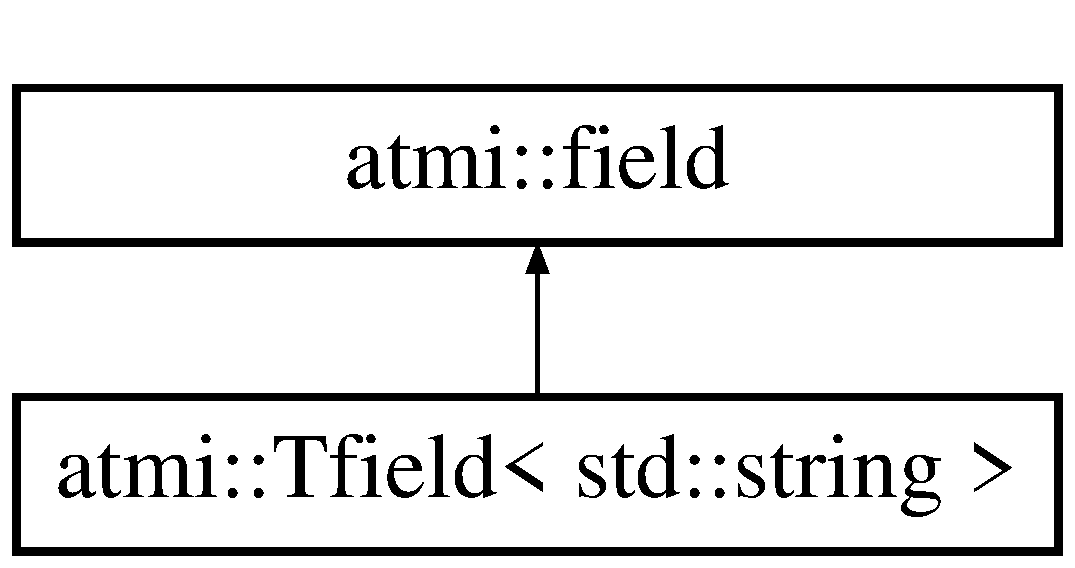
\includegraphics[height=2.000000cm]{classatmi_1_1_tfield_3_01std_1_1string_01_4}
\end{center}
\end{figure}
\subsection*{Public Member Functions}
\begin{DoxyCompactItemize}
\item 
\hyperlink{classatmi_1_1_tfield_3_01std_1_1string_01_4_a46059c3e91ce3847b3109e4500f017f6}{Tfield} (F\+L\+D\+I\+D32 fid)
\item 
\hyperlink{classatmi_1_1_tfield_3_01std_1_1string_01_4_ac228a4c4d13e1573fd166a6506d98d87}{Tfield} (const char $\ast$n)
\item 
virtual F\+L\+D\+L\+E\+N32 \hyperlink{classatmi_1_1_tfield_3_01std_1_1string_01_4_ac4fdf6b5f9d1929b34bddc97274c6c9b}{length} ()
\item 
virtual F\+L\+D\+L\+E\+N32 \hyperlink{classatmi_1_1_tfield_3_01std_1_1string_01_4_aea88f61cd27f8f258ee473e0e938790b}{size} ()
\item 
const char $\ast$ \hyperlink{classatmi_1_1_tfield_3_01std_1_1string_01_4_a775ddd0103e3e3f0fc85dfda5df72280}{c\+\_\+str} () const 
\item 
string \& \hyperlink{classatmi_1_1_tfield_3_01std_1_1string_01_4_a95b55ca60414937f64af4705e7f8da08}{operator+=} (const string \&str)
\item 
string \& \hyperlink{classatmi_1_1_tfield_3_01std_1_1string_01_4_aa72122815bb188213438681fca0bb016}{operator+=} (const char $\ast$s)
\item 
string \& \hyperlink{classatmi_1_1_tfield_3_01std_1_1string_01_4_abf76ab2b474fc6b4500d3d9c57b0c083}{operator+=} (char c)
\item 
const char \& \hyperlink{classatmi_1_1_tfield_3_01std_1_1string_01_4_aeff4f32e684575375cff733f3838d8bc}{operator\mbox{[}$\,$\mbox{]}} (size\+\_\+t pos) const 
\item 
char \& \hyperlink{classatmi_1_1_tfield_3_01std_1_1string_01_4_a21a1c27750ed6b7d61695350e222454b}{operator\mbox{[}$\,$\mbox{]}} (size\+\_\+t pos)
\item 
virtual \hyperlink{classatmi_1_1_tfield}{Tfield}$<$ string $>$ \& \hyperlink{classatmi_1_1_tfield_3_01std_1_1string_01_4_a2d925169a3c28b5bcbcb62b0c3834f41}{operator=} (const char $\ast$str)
\item 
virtual \hyperlink{classatmi_1_1_tfield}{Tfield}$<$ string $>$ \& \hyperlink{classatmi_1_1_tfield_3_01std_1_1string_01_4_ad9da8df81976f159a95bd5729032fb42}{operator=} (const string \&str)
\item 
virtual \hyperlink{classatmi_1_1_tfield}{Tfield}$<$ string $>$ \& \hyperlink{classatmi_1_1_tfield_3_01std_1_1string_01_4_a9a1f850dc223743e8a498d25a93b3af9}{operator=} (char \&c)
\item 
\hyperlink{classatmi_1_1_tfield_3_01std_1_1string_01_4_a134b213194d5e1cda743d588e3c219e2}{operator string} ()
\end{DoxyCompactItemize}
\subsection*{Protected Member Functions}
\begin{DoxyCompactItemize}
\item 
virtual int \hyperlink{classatmi_1_1_tfield_3_01std_1_1string_01_4_a356a0e794a33bcfc1d3f4d8376e764d9}{set} (\hyperlink{classatmi_1_1buffer}{buffer} \&b)
\item 
virtual int \hyperlink{classatmi_1_1_tfield_3_01std_1_1string_01_4_af17fc3c22ce857f9d96f96d6c175b6d5}{add} (\hyperlink{classatmi_1_1buffer}{buffer} \&b)
\item 
virtual int \hyperlink{classatmi_1_1_tfield_3_01std_1_1string_01_4_afecf8218a3c312df34c36f334c995ac7}{get} (\hyperlink{classatmi_1_1buffer}{buffer} \&b)
\item 
virtual int \hyperlink{classatmi_1_1_tfield_3_01std_1_1string_01_4_a34f9956af4b0b98730595258e6c251e2}{get} (\hyperlink{classatmi_1_1buffer}{buffer} \&b, F\+L\+D\+O\+C\+C32 occ)
\end{DoxyCompactItemize}
\subsection*{Protected Attributes}
\begin{DoxyCompactItemize}
\item 
\hypertarget{classatmi_1_1_tfield_3_01std_1_1string_01_4_a8c0e9d6d6ef699d221ef18fb0a048230}{string \hyperlink{classatmi_1_1_tfield_3_01std_1_1string_01_4_a8c0e9d6d6ef699d221ef18fb0a048230}{value}}\label{classatmi_1_1_tfield_3_01std_1_1string_01_4_a8c0e9d6d6ef699d221ef18fb0a048230}

\begin{DoxyCompactList}\small\item\em string field's value \end{DoxyCompactList}\end{DoxyCompactItemize}


\subsection{Detailed Description}
\subsubsection*{template$<$$>$class atmi\+::\+Tfield$<$ std\+::string $>$}



Specialization of template \hyperlink{classatmi_1_1_tfield}{Tfield} which handles string typed fields.

This class is using a string object to hold and handle string data When a new instance is created, occurence is set to 0 making it possible to set values withour a prior call to add. 

\subsection{Constructor \& Destructor Documentation}
\hypertarget{classatmi_1_1_tfield_3_01std_1_1string_01_4_a46059c3e91ce3847b3109e4500f017f6}{\index{atmi\+::\+Tfield$<$ std\+::string $>$@{atmi\+::\+Tfield$<$ std\+::string $>$}!Tfield@{Tfield}}
\index{Tfield@{Tfield}!atmi\+::\+Tfield$<$ std\+::string $>$@{atmi\+::\+Tfield$<$ std\+::string $>$}}
\subsubsection[{Tfield}]{\setlength{\rightskip}{0pt plus 5cm}{\bf atmi\+::\+Tfield}$<$ std\+::string $>$\+::{\bf Tfield} (
\begin{DoxyParamCaption}
\item[{F\+L\+D\+I\+D32}]{fid}
\end{DoxyParamCaption}
)\hspace{0.3cm}{\ttfamily [inline]}, {\ttfamily [explicit]}}}\label{classatmi_1_1_tfield_3_01std_1_1string_01_4_a46059c3e91ce3847b3109e4500f017f6}
Constructs a \hyperlink{classatmi_1_1_tfield}{Tfield} for the passed field id

The search is done in the tables identified by F\+L\+D\+T\+B\+L\+D\+I\+R32 and F\+I\+E\+L\+D\+T\+B\+L\+S32


\begin{DoxyParams}{Parameters}
{\em fid} & the fml field id to setup (as defined in the F\+M\+L tables) \\
\hline
\end{DoxyParams}
\hypertarget{classatmi_1_1_tfield_3_01std_1_1string_01_4_ac228a4c4d13e1573fd166a6506d98d87}{\index{atmi\+::\+Tfield$<$ std\+::string $>$@{atmi\+::\+Tfield$<$ std\+::string $>$}!Tfield@{Tfield}}
\index{Tfield@{Tfield}!atmi\+::\+Tfield$<$ std\+::string $>$@{atmi\+::\+Tfield$<$ std\+::string $>$}}
\subsubsection[{Tfield}]{\setlength{\rightskip}{0pt plus 5cm}{\bf atmi\+::\+Tfield}$<$ std\+::string $>$\+::{\bf Tfield} (
\begin{DoxyParamCaption}
\item[{const char $\ast$}]{n}
\end{DoxyParamCaption}
)\hspace{0.3cm}{\ttfamily [inline]}, {\ttfamily [explicit]}}}\label{classatmi_1_1_tfield_3_01std_1_1string_01_4_ac228a4c4d13e1573fd166a6506d98d87}
Constructs a \hyperlink{classatmi_1_1_tfield}{Tfield} for the passed name

The search is done in the tables identified by F\+L\+D\+T\+B\+L\+D\+I\+R32 and F\+I\+E\+L\+D\+T\+B\+L\+S32


\begin{DoxyParams}{Parameters}
{\em n} & the fml field name to setup (as defined in the F\+M\+L tables) \\
\hline
\end{DoxyParams}


\subsection{Member Function Documentation}
\hypertarget{classatmi_1_1_tfield_3_01std_1_1string_01_4_af17fc3c22ce857f9d96f96d6c175b6d5}{\index{atmi\+::\+Tfield$<$ std\+::string $>$@{atmi\+::\+Tfield$<$ std\+::string $>$}!add@{add}}
\index{add@{add}!atmi\+::\+Tfield$<$ std\+::string $>$@{atmi\+::\+Tfield$<$ std\+::string $>$}}
\subsubsection[{add}]{\setlength{\rightskip}{0pt plus 5cm}virtual int {\bf atmi\+::\+Tfield}$<$ std\+::string $>$\+::add (
\begin{DoxyParamCaption}
\item[{{\bf buffer} \&}]{b}
\end{DoxyParamCaption}
)\hspace{0.3cm}{\ttfamily [inline]}, {\ttfamily [protected]}, {\ttfamily [virtual]}}}\label{classatmi_1_1_tfield_3_01std_1_1string_01_4_af17fc3c22ce857f9d96f96d6c175b6d5}
add the fiels into the buffer

When successfull the value of occurence is set


\begin{DoxyParams}{Parameters}
{\em b} & buffer in which to add the field. \\
\hline
\end{DoxyParams}
\begin{DoxySeeAlso}{See also}
\hyperlink{classatmi_1_1field_a161b9b7037c49fbcf86518fcb35e779c}{occurence} 
\end{DoxySeeAlso}


Implements \hyperlink{classatmi_1_1field_a5441bc87ba4bc3e9eb37c6db6a29688f}{atmi\+::field}.

\hypertarget{classatmi_1_1_tfield_3_01std_1_1string_01_4_a775ddd0103e3e3f0fc85dfda5df72280}{\index{atmi\+::\+Tfield$<$ std\+::string $>$@{atmi\+::\+Tfield$<$ std\+::string $>$}!c\+\_\+str@{c\+\_\+str}}
\index{c\+\_\+str@{c\+\_\+str}!atmi\+::\+Tfield$<$ std\+::string $>$@{atmi\+::\+Tfield$<$ std\+::string $>$}}
\subsubsection[{c\+\_\+str}]{\setlength{\rightskip}{0pt plus 5cm}const char$\ast$ {\bf atmi\+::\+Tfield}$<$ std\+::string $>$\+::c\+\_\+str (
\begin{DoxyParamCaption}
{}
\end{DoxyParamCaption}
) const\hspace{0.3cm}{\ttfamily [inline]}}}\label{classatmi_1_1_tfield_3_01std_1_1string_01_4_a775ddd0103e3e3f0fc85dfda5df72280}
\begin{DoxyReturn}{Returns}
a C string (with \textbackslash{}0) of current string's content. 
\end{DoxyReturn}
\hypertarget{classatmi_1_1_tfield_3_01std_1_1string_01_4_afecf8218a3c312df34c36f334c995ac7}{\index{atmi\+::\+Tfield$<$ std\+::string $>$@{atmi\+::\+Tfield$<$ std\+::string $>$}!get@{get}}
\index{get@{get}!atmi\+::\+Tfield$<$ std\+::string $>$@{atmi\+::\+Tfield$<$ std\+::string $>$}}
\subsubsection[{get}]{\setlength{\rightskip}{0pt plus 5cm}virtual int {\bf atmi\+::\+Tfield}$<$ std\+::string $>$\+::get (
\begin{DoxyParamCaption}
\item[{{\bf buffer} \&}]{b}
\end{DoxyParamCaption}
)\hspace{0.3cm}{\ttfamily [inline]}, {\ttfamily [protected]}, {\ttfamily [virtual]}}}\label{classatmi_1_1_tfield_3_01std_1_1string_01_4_afecf8218a3c312df34c36f334c995ac7}
Retrieves the value of the field found into the buffer.


\begin{DoxyParams}{Parameters}
{\em b} & buffer from which to retrieve the field's value \\
\hline
\end{DoxyParams}


Implements \hyperlink{classatmi_1_1field_aae2d3df756e816b5db8f729039a59a51}{atmi\+::field}.

\hypertarget{classatmi_1_1_tfield_3_01std_1_1string_01_4_a34f9956af4b0b98730595258e6c251e2}{\index{atmi\+::\+Tfield$<$ std\+::string $>$@{atmi\+::\+Tfield$<$ std\+::string $>$}!get@{get}}
\index{get@{get}!atmi\+::\+Tfield$<$ std\+::string $>$@{atmi\+::\+Tfield$<$ std\+::string $>$}}
\subsubsection[{get}]{\setlength{\rightskip}{0pt plus 5cm}virtual int {\bf atmi\+::\+Tfield}$<$ std\+::string $>$\+::get (
\begin{DoxyParamCaption}
\item[{{\bf buffer} \&}]{b, }
\item[{F\+L\+D\+O\+C\+C32}]{occ}
\end{DoxyParamCaption}
)\hspace{0.3cm}{\ttfamily [inline]}, {\ttfamily [protected]}, {\ttfamily [virtual]}}}\label{classatmi_1_1_tfield_3_01std_1_1string_01_4_a34f9956af4b0b98730595258e6c251e2}
Retrieves the value of the field's occurence found into the buffer

Upon success the value of occurence is set to the retrieved occurence.


\begin{DoxyParams}{Parameters}
{\em b} & buffer from which to retrieve the field's value \\
\hline
{\em occ} & occurence to retreive \\
\hline
\end{DoxyParams}
\begin{DoxySeeAlso}{See also}
\hyperlink{classatmi_1_1field_a161b9b7037c49fbcf86518fcb35e779c}{occurence} 
\end{DoxySeeAlso}


Implements \hyperlink{classatmi_1_1field_a56ce53fabe290b94463f87936515ec46}{atmi\+::field}.

\hypertarget{classatmi_1_1_tfield_3_01std_1_1string_01_4_ac4fdf6b5f9d1929b34bddc97274c6c9b}{\index{atmi\+::\+Tfield$<$ std\+::string $>$@{atmi\+::\+Tfield$<$ std\+::string $>$}!length@{length}}
\index{length@{length}!atmi\+::\+Tfield$<$ std\+::string $>$@{atmi\+::\+Tfield$<$ std\+::string $>$}}
\subsubsection[{length}]{\setlength{\rightskip}{0pt plus 5cm}virtual F\+L\+D\+L\+E\+N32 {\bf atmi\+::\+Tfield}$<$ std\+::string $>$\+::length (
\begin{DoxyParamCaption}
{}
\end{DoxyParamCaption}
)\hspace{0.3cm}{\ttfamily [inline]}, {\ttfamily [virtual]}}}\label{classatmi_1_1_tfield_3_01std_1_1string_01_4_ac4fdf6b5f9d1929b34bddc97274c6c9b}
\begin{DoxyReturn}{Returns}
the string's length 
\end{DoxyReturn}


Implements \hyperlink{classatmi_1_1field_a296771293135085d91aa9aefd108d44d}{atmi\+::field}.

\hypertarget{classatmi_1_1_tfield_3_01std_1_1string_01_4_a134b213194d5e1cda743d588e3c219e2}{\index{atmi\+::\+Tfield$<$ std\+::string $>$@{atmi\+::\+Tfield$<$ std\+::string $>$}!operator string@{operator string}}
\index{operator string@{operator string}!atmi\+::\+Tfield$<$ std\+::string $>$@{atmi\+::\+Tfield$<$ std\+::string $>$}}
\subsubsection[{operator string}]{\setlength{\rightskip}{0pt plus 5cm}{\bf atmi\+::\+Tfield}$<$ std\+::string $>$\+::operator string (
\begin{DoxyParamCaption}
{}
\end{DoxyParamCaption}
)\hspace{0.3cm}{\ttfamily [inline]}}}\label{classatmi_1_1_tfield_3_01std_1_1string_01_4_a134b213194d5e1cda743d588e3c219e2}
casts the field value \hypertarget{classatmi_1_1_tfield_3_01std_1_1string_01_4_a95b55ca60414937f64af4705e7f8da08}{\index{atmi\+::\+Tfield$<$ std\+::string $>$@{atmi\+::\+Tfield$<$ std\+::string $>$}!operator+=@{operator+=}}
\index{operator+=@{operator+=}!atmi\+::\+Tfield$<$ std\+::string $>$@{atmi\+::\+Tfield$<$ std\+::string $>$}}
\subsubsection[{operator+=}]{\setlength{\rightskip}{0pt plus 5cm}string\& {\bf atmi\+::\+Tfield}$<$ std\+::string $>$\+::operator+= (
\begin{DoxyParamCaption}
\item[{const string \&}]{str}
\end{DoxyParamCaption}
)\hspace{0.3cm}{\ttfamily [inline]}}}\label{classatmi_1_1_tfield_3_01std_1_1string_01_4_a95b55ca60414937f64af4705e7f8da08}
Appends a copy of the argument to the string.

The new string content is the content existing in the string object before the call followed by the content of the argument.

The append member function provides a similar functionality with additional options.


\begin{DoxyParams}{Parameters}
{\em str} & a copy of the content of this object is appended to the object's content. \\
\hline
\end{DoxyParams}
\begin{DoxyReturn}{Returns}
$\ast$this 
\end{DoxyReturn}
\hypertarget{classatmi_1_1_tfield_3_01std_1_1string_01_4_aa72122815bb188213438681fca0bb016}{\index{atmi\+::\+Tfield$<$ std\+::string $>$@{atmi\+::\+Tfield$<$ std\+::string $>$}!operator+=@{operator+=}}
\index{operator+=@{operator+=}!atmi\+::\+Tfield$<$ std\+::string $>$@{atmi\+::\+Tfield$<$ std\+::string $>$}}
\subsubsection[{operator+=}]{\setlength{\rightskip}{0pt plus 5cm}string\& {\bf atmi\+::\+Tfield}$<$ std\+::string $>$\+::operator+= (
\begin{DoxyParamCaption}
\item[{const char $\ast$}]{s}
\end{DoxyParamCaption}
)\hspace{0.3cm}{\ttfamily [inline]}}}\label{classatmi_1_1_tfield_3_01std_1_1string_01_4_aa72122815bb188213438681fca0bb016}
Appends a copy of the argument to the string.

The new string content is the content existing in the string object before the call followed by the content of the argument.

The append member function provides a similar functionality with additional options.


\begin{DoxyParams}{Parameters}
{\em s} & a pointer to an array containing a null-\/terminated character sequence (C string), which is appended to the object's content. \\
\hline
\end{DoxyParams}
\begin{DoxyReturn}{Returns}
$\ast$this 
\end{DoxyReturn}
\hypertarget{classatmi_1_1_tfield_3_01std_1_1string_01_4_abf76ab2b474fc6b4500d3d9c57b0c083}{\index{atmi\+::\+Tfield$<$ std\+::string $>$@{atmi\+::\+Tfield$<$ std\+::string $>$}!operator+=@{operator+=}}
\index{operator+=@{operator+=}!atmi\+::\+Tfield$<$ std\+::string $>$@{atmi\+::\+Tfield$<$ std\+::string $>$}}
\subsubsection[{operator+=}]{\setlength{\rightskip}{0pt plus 5cm}string\& {\bf atmi\+::\+Tfield}$<$ std\+::string $>$\+::operator+= (
\begin{DoxyParamCaption}
\item[{char}]{c}
\end{DoxyParamCaption}
)\hspace{0.3cm}{\ttfamily [inline]}}}\label{classatmi_1_1_tfield_3_01std_1_1string_01_4_abf76ab2b474fc6b4500d3d9c57b0c083}
Appends character to the string field.


\begin{DoxyParams}{Parameters}
{\em c} & character. This single character is appended to the string object's content. \\
\hline
\end{DoxyParams}
\begin{DoxyReturn}{Returns}
$\ast$this 
\end{DoxyReturn}
\hypertarget{classatmi_1_1_tfield_3_01std_1_1string_01_4_a2d925169a3c28b5bcbcb62b0c3834f41}{\index{atmi\+::\+Tfield$<$ std\+::string $>$@{atmi\+::\+Tfield$<$ std\+::string $>$}!operator=@{operator=}}
\index{operator=@{operator=}!atmi\+::\+Tfield$<$ std\+::string $>$@{atmi\+::\+Tfield$<$ std\+::string $>$}}
\subsubsection[{operator=}]{\setlength{\rightskip}{0pt plus 5cm}virtual {\bf Tfield}$<$string$>$\& {\bf atmi\+::\+Tfield}$<$ std\+::string $>$\+::operator= (
\begin{DoxyParamCaption}
\item[{const char $\ast$}]{str}
\end{DoxyParamCaption}
)\hspace{0.3cm}{\ttfamily [inline]}, {\ttfamily [virtual]}}}\label{classatmi_1_1_tfield_3_01std_1_1string_01_4_a2d925169a3c28b5bcbcb62b0c3834f41}
assigns values to the string field.


\begin{DoxyParams}{Parameters}
{\em str} & null terminated character array. \\
\hline
\end{DoxyParams}
\hypertarget{classatmi_1_1_tfield_3_01std_1_1string_01_4_ad9da8df81976f159a95bd5729032fb42}{\index{atmi\+::\+Tfield$<$ std\+::string $>$@{atmi\+::\+Tfield$<$ std\+::string $>$}!operator=@{operator=}}
\index{operator=@{operator=}!atmi\+::\+Tfield$<$ std\+::string $>$@{atmi\+::\+Tfield$<$ std\+::string $>$}}
\subsubsection[{operator=}]{\setlength{\rightskip}{0pt plus 5cm}virtual {\bf Tfield}$<$string$>$\& {\bf atmi\+::\+Tfield}$<$ std\+::string $>$\+::operator= (
\begin{DoxyParamCaption}
\item[{const string \&}]{str}
\end{DoxyParamCaption}
)\hspace{0.3cm}{\ttfamily [inline]}, {\ttfamily [virtual]}}}\label{classatmi_1_1_tfield_3_01std_1_1string_01_4_ad9da8df81976f159a95bd5729032fb42}
assigns values to the string field.


\begin{DoxyParams}{Parameters}
{\em str} & string to assign \\
\hline
\end{DoxyParams}


Reimplemented from \hyperlink{classatmi_1_1field_ac032afae0c1ebfc606f047ce1a32ac58}{atmi\+::field}.

\hypertarget{classatmi_1_1_tfield_3_01std_1_1string_01_4_a9a1f850dc223743e8a498d25a93b3af9}{\index{atmi\+::\+Tfield$<$ std\+::string $>$@{atmi\+::\+Tfield$<$ std\+::string $>$}!operator=@{operator=}}
\index{operator=@{operator=}!atmi\+::\+Tfield$<$ std\+::string $>$@{atmi\+::\+Tfield$<$ std\+::string $>$}}
\subsubsection[{operator=}]{\setlength{\rightskip}{0pt plus 5cm}virtual {\bf Tfield}$<$string$>$\& {\bf atmi\+::\+Tfield}$<$ std\+::string $>$\+::operator= (
\begin{DoxyParamCaption}
\item[{char \&}]{c}
\end{DoxyParamCaption}
)\hspace{0.3cm}{\ttfamily [inline]}, {\ttfamily [virtual]}}}\label{classatmi_1_1_tfield_3_01std_1_1string_01_4_a9a1f850dc223743e8a498d25a93b3af9}
assigns values to the string field.


\begin{DoxyParams}{Parameters}
{\em c} & the content is set to a single character. \\
\hline
\end{DoxyParams}
\hypertarget{classatmi_1_1_tfield_3_01std_1_1string_01_4_aeff4f32e684575375cff733f3838d8bc}{\index{atmi\+::\+Tfield$<$ std\+::string $>$@{atmi\+::\+Tfield$<$ std\+::string $>$}!operator\mbox{[}$\,$\mbox{]}@{operator[]}}
\index{operator\mbox{[}$\,$\mbox{]}@{operator[]}!atmi\+::\+Tfield$<$ std\+::string $>$@{atmi\+::\+Tfield$<$ std\+::string $>$}}
\subsubsection[{operator[]}]{\setlength{\rightskip}{0pt plus 5cm}const char\& {\bf atmi\+::\+Tfield}$<$ std\+::string $>$\+::operator\mbox{[}$\,$\mbox{]} (
\begin{DoxyParamCaption}
\item[{size\+\_\+t}]{pos}
\end{DoxyParamCaption}
) const\hspace{0.3cm}{\ttfamily [inline]}}}\label{classatmi_1_1_tfield_3_01std_1_1string_01_4_aeff4f32e684575375cff733f3838d8bc}
Returns a reference the character at position pos in the string.

The function actually returns data()\mbox{[} pos \mbox{]}.

The at member function has the same behavior as this operator function, except that at also performs a range check.


\begin{DoxyParams}{Parameters}
{\em pos} & position within the string of the character to be retrieved. Notice that the first character in the string has a position of 0, not 1. size\+\_\+t is an unsigned integral type. \\
\hline
\end{DoxyParams}
\begin{DoxyReturn}{Returns}
The character at the specified position in the string. 
\end{DoxyReturn}
\hypertarget{classatmi_1_1_tfield_3_01std_1_1string_01_4_a21a1c27750ed6b7d61695350e222454b}{\index{atmi\+::\+Tfield$<$ std\+::string $>$@{atmi\+::\+Tfield$<$ std\+::string $>$}!operator\mbox{[}$\,$\mbox{]}@{operator[]}}
\index{operator\mbox{[}$\,$\mbox{]}@{operator[]}!atmi\+::\+Tfield$<$ std\+::string $>$@{atmi\+::\+Tfield$<$ std\+::string $>$}}
\subsubsection[{operator[]}]{\setlength{\rightskip}{0pt plus 5cm}char\& {\bf atmi\+::\+Tfield}$<$ std\+::string $>$\+::operator\mbox{[}$\,$\mbox{]} (
\begin{DoxyParamCaption}
\item[{size\+\_\+t}]{pos}
\end{DoxyParamCaption}
)\hspace{0.3cm}{\ttfamily [inline]}}}\label{classatmi_1_1_tfield_3_01std_1_1string_01_4_a21a1c27750ed6b7d61695350e222454b}
Returns a reference the character at position pos in the string.

The function actually returns data()\mbox{[} pos \mbox{]}.

The at member function has the same behavior as this operator function, except that at also performs a range check.


\begin{DoxyParams}{Parameters}
{\em pos} & position within the string of the character to be retrieved. Notice that the first character in the string has a position of 0, not 1. size\+\_\+t is an unsigned integral type. \\
\hline
\end{DoxyParams}
\begin{DoxyReturn}{Returns}
The character at the specified position in the string. 
\end{DoxyReturn}
\hypertarget{classatmi_1_1_tfield_3_01std_1_1string_01_4_a356a0e794a33bcfc1d3f4d8376e764d9}{\index{atmi\+::\+Tfield$<$ std\+::string $>$@{atmi\+::\+Tfield$<$ std\+::string $>$}!set@{set}}
\index{set@{set}!atmi\+::\+Tfield$<$ std\+::string $>$@{atmi\+::\+Tfield$<$ std\+::string $>$}}
\subsubsection[{set}]{\setlength{\rightskip}{0pt plus 5cm}virtual int {\bf atmi\+::\+Tfield}$<$ std\+::string $>$\+::set (
\begin{DoxyParamCaption}
\item[{{\bf buffer} \&}]{b}
\end{DoxyParamCaption}
)\hspace{0.3cm}{\ttfamily [inline]}, {\ttfamily [protected]}, {\ttfamily [virtual]}}}\label{classatmi_1_1_tfield_3_01std_1_1string_01_4_a356a0e794a33bcfc1d3f4d8376e764d9}
set the value of the field's value


\begin{DoxyParams}{Parameters}
{\em b} & the buffer in which the value must be changed \\
\hline
\end{DoxyParams}


Implements \hyperlink{classatmi_1_1field_a41bb209965d627d2e67c839bece5372c}{atmi\+::field}.

\hypertarget{classatmi_1_1_tfield_3_01std_1_1string_01_4_aea88f61cd27f8f258ee473e0e938790b}{\index{atmi\+::\+Tfield$<$ std\+::string $>$@{atmi\+::\+Tfield$<$ std\+::string $>$}!size@{size}}
\index{size@{size}!atmi\+::\+Tfield$<$ std\+::string $>$@{atmi\+::\+Tfield$<$ std\+::string $>$}}
\subsubsection[{size}]{\setlength{\rightskip}{0pt plus 5cm}virtual F\+L\+D\+L\+E\+N32 {\bf atmi\+::\+Tfield}$<$ std\+::string $>$\+::size (
\begin{DoxyParamCaption}
{}
\end{DoxyParamCaption}
)\hspace{0.3cm}{\ttfamily [inline]}, {\ttfamily [virtual]}}}\label{classatmi_1_1_tfield_3_01std_1_1string_01_4_aea88f61cd27f8f258ee473e0e938790b}
\begin{DoxyReturn}{Returns}
the string's size 
\end{DoxyReturn}


The documentation for this class was generated from the following file\+:\begin{DoxyCompactItemize}
\item 
include/atmi/fields.\+hpp\end{DoxyCompactItemize}

\hypertarget{classatmi_1_1timeout__exception}{\section{atmi\+:\+:timeout\+\_\+exception Class Reference}
\label{classatmi_1_1timeout__exception}\index{atmi\+::timeout\+\_\+exception@{atmi\+::timeout\+\_\+exception}}
}


{\ttfamily \#include $<$exceptions.\+hpp$>$}

Inheritance diagram for atmi\+:\+:timeout\+\_\+exception\+:\begin{figure}[H]
\begin{center}
\leavevmode
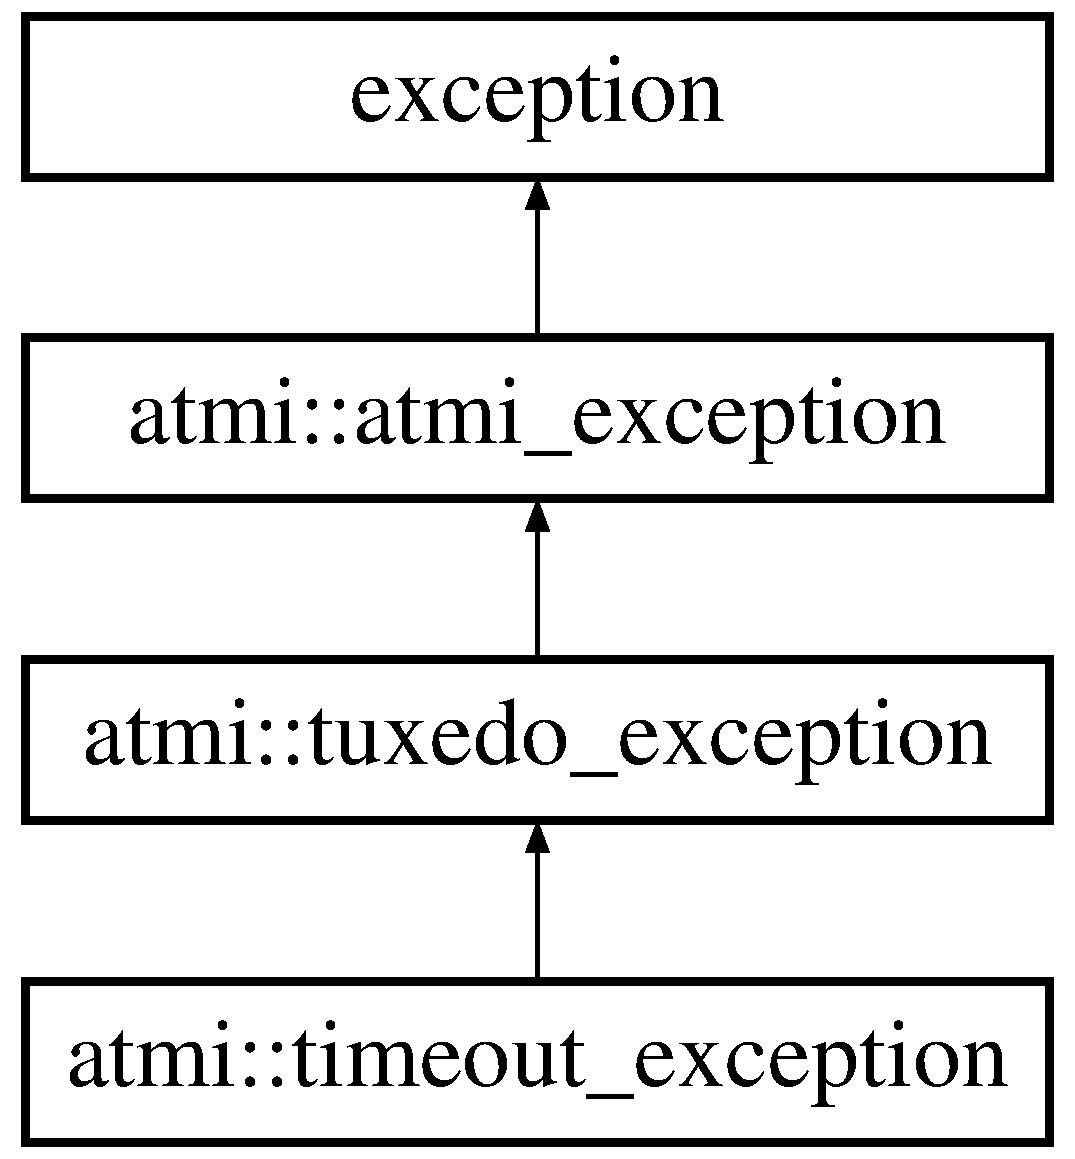
\includegraphics[height=4.000000cm]{classatmi_1_1timeout__exception}
\end{center}
\end{figure}
\subsection*{Public Member Functions}
\begin{DoxyCompactItemize}
\item 
{\footnotesize template$<$typename... Args$>$ }\\\hyperlink{classatmi_1_1timeout__exception_a8fe65e08189bb4d6cbcd63bbfdb53a2b}{timeout\+\_\+exception} (const char $\ast$msg, const Args \&...args)
\end{DoxyCompactItemize}
\subsection*{Additional Inherited Members}


\subsection{Detailed Description}
Thrown when T\+P\+E\+T\+I\+M\+E is returned after a T\+P call. 

\subsection{Constructor \& Destructor Documentation}
\hypertarget{classatmi_1_1timeout__exception_a8fe65e08189bb4d6cbcd63bbfdb53a2b}{\index{atmi\+::timeout\+\_\+exception@{atmi\+::timeout\+\_\+exception}!timeout\+\_\+exception@{timeout\+\_\+exception}}
\index{timeout\+\_\+exception@{timeout\+\_\+exception}!atmi\+::timeout\+\_\+exception@{atmi\+::timeout\+\_\+exception}}
\subsubsection[{timeout\+\_\+exception}]{\setlength{\rightskip}{0pt plus 5cm}template$<$typename... Args$>$ atmi\+::timeout\+\_\+exception\+::timeout\+\_\+exception (
\begin{DoxyParamCaption}
\item[{const char $\ast$}]{msg, }
\item[{const Args \&...}]{args}
\end{DoxyParamCaption}
)\hspace{0.3cm}{\ttfamily [inline]}}}\label{classatmi_1_1timeout__exception_a8fe65e08189bb4d6cbcd63bbfdb53a2b}
new instance.


\begin{DoxyParams}{Parameters}
{\em msg} & error message \\
\hline
{\em args} & error message parameters (variadic). \\
\hline
\end{DoxyParams}


The documentation for this class was generated from the following file\+:\begin{DoxyCompactItemize}
\item 
include/atmi/exceptions.\+hpp\end{DoxyCompactItemize}

\hypertarget{classatmi_1_1transaction}{}\section{atmi\+:\+:transaction Class Reference}
\label{classatmi_1_1transaction}\index{atmi\+::transaction@{atmi\+::transaction}}


{\ttfamily \#include $<$transaction.\+hpp$>$}

Inheritance diagram for atmi\+:\+:transaction\+:\begin{figure}[H]
\begin{center}
\leavevmode
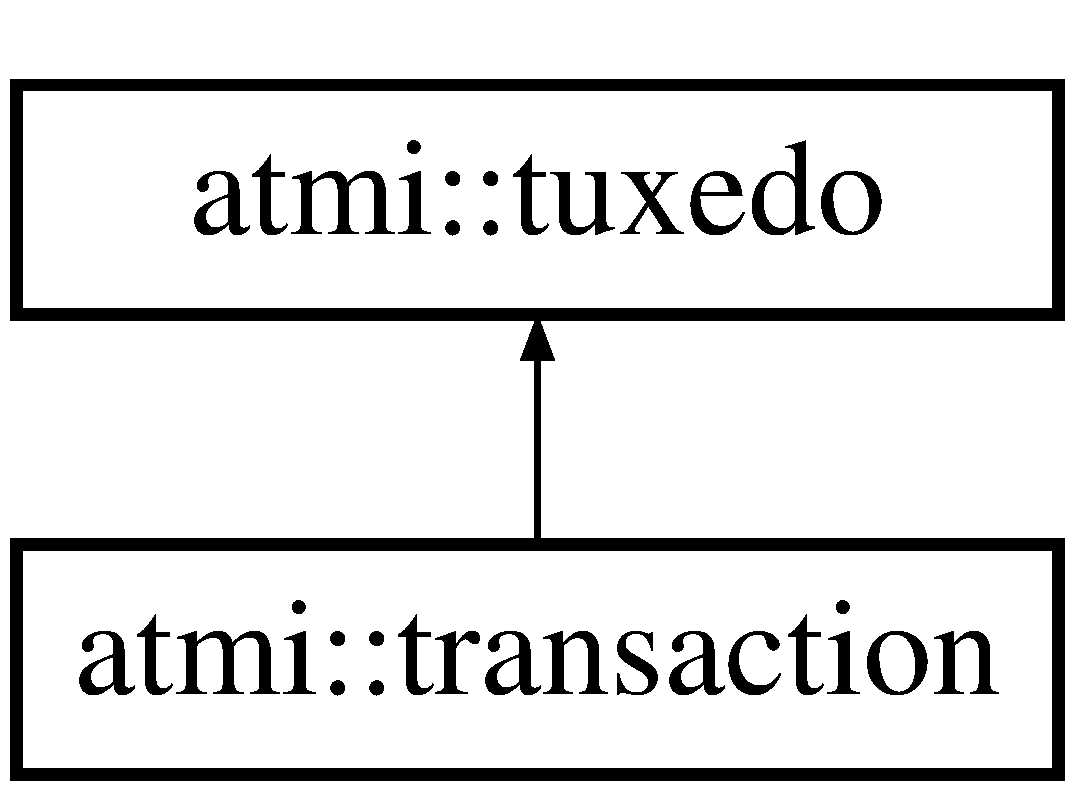
\includegraphics[height=2.000000cm]{classatmi_1_1transaction}
\end{center}
\end{figure}
\subsection*{Public Member Functions}
\begin{DoxyCompactItemize}
\item 
int \hyperlink{classatmi_1_1transaction_a1251381692ec4e235ca9179a84273484}{call} (char $\ast$idata, long ilen, char $\ast$$\ast$odata, long $\ast$olen, int $\ast$urcode=N\+U\+LL, int retries=0, int delay=0)
\item 
int \hyperlink{classatmi_1_1transaction_afc2bebb88fb56466d0a41d45e6060377}{call} (\hyperlink{classatmi_1_1buffer}{buffer} \&\hyperlink{classatmi_1_1buffer}{buffer}, int $\ast$urcode=N\+U\+LL, int retries=0, int delay=0)
\item 
int \hyperlink{classatmi_1_1transaction_aa5fb9edab0ee78c39b73936ca59a0b02}{call} (char $\ast$$\ast$idata=N\+U\+LL, long $\ast$ilen=0, int $\ast$urcode=N\+U\+LL, int retries=0, int delay=0)
\item 
int \hyperlink{classatmi_1_1transaction_abf3ecf74af155274d4b500df2e6ec69b}{acall} (char $\ast$idata=N\+U\+LL, long ilen=0)
\item 
int \hyperlink{classatmi_1_1transaction_a3abfbaad23aafaccd6b96af66d36e329}{acall} (\hyperlink{classatmi_1_1buffer}{buffer} \&\hyperlink{classatmi_1_1buffer}{buffer})
\item 
int \hyperlink{classatmi_1_1transaction_a810c7fdad2bc26722027d4d0565f4c9a}{reply} (char $\ast$$\ast$data, long $\ast$len, int $\ast$urcode=N\+U\+LL, int $\ast$cd=N\+U\+LL)
\item 
int \hyperlink{classatmi_1_1transaction_a3bcbf7ec6d3b9909e10368ffb6e3d39d}{reply} (\hyperlink{classatmi_1_1buffer}{buffer} \&\hyperlink{classatmi_1_1buffer}{buffer}, int $\ast$urcode=N\+U\+LL, int $\ast$cd=N\+U\+LL)
\item 
int \hyperlink{classatmi_1_1transaction_a380d536258d33a801973100d6e2ae622}{cancel} (int cd=0)
\item 
int \hyperlink{classatmi_1_1transaction_a11018dd9689a5a66d0510ae78bb048da}{call\+\_\+descriptor} ()
\item 
string \hyperlink{classatmi_1_1transaction_a16d4442ea8f6582ec4820a064fc9a825}{service} ()
\item 
\hyperlink{classatmi_1_1transaction_a0cb59a4954d3fc4b903c0f2876dd00b3}{transaction} (const char $\ast$\hyperlink{classatmi_1_1transaction_a16d4442ea8f6582ec4820a064fc9a825}{service})
\end{DoxyCompactItemize}
\subsection*{Additional Inherited Members}


\subsection{Detailed Description}
Implement transaction calls (/T)

\begin{DoxyAuthor}{Author}
herbert koelman 
\end{DoxyAuthor}


\subsection{Constructor \& Destructor Documentation}
\index{atmi\+::transaction@{atmi\+::transaction}!transaction@{transaction}}
\index{transaction@{transaction}!atmi\+::transaction@{atmi\+::transaction}}
\subsubsection[{\texorpdfstring{transaction(const char $\ast$service)}{transaction(const char *service)}}]{\setlength{\rightskip}{0pt plus 5cm}atmi\+::transaction\+::transaction (
\begin{DoxyParamCaption}
\item[{const char $\ast$}]{service}
\end{DoxyParamCaption}
)\hspace{0.3cm}{\ttfamily [explicit]}}\hypertarget{classatmi_1_1transaction_a0cb59a4954d3fc4b903c0f2876dd00b3}{}\label{classatmi_1_1transaction_a0cb59a4954d3fc4b903c0f2876dd00b3}

\begin{DoxyParams}{Parameters}
{\em service} & service name ($<$ 32 characters long) \\
\hline
\end{DoxyParams}


\subsection{Member Function Documentation}
\index{atmi\+::transaction@{atmi\+::transaction}!acall@{acall}}
\index{acall@{acall}!atmi\+::transaction@{atmi\+::transaction}}
\subsubsection[{\texorpdfstring{acall(char $\ast$idata=\+N\+U\+L\+L, long ilen=0)}{acall(char *idata=NULL, long ilen=0)}}]{\setlength{\rightskip}{0pt plus 5cm}int atmi\+::transaction\+::acall (
\begin{DoxyParamCaption}
\item[{char $\ast$}]{idata = {\ttfamily NULL}, }
\item[{long}]{ilen = {\ttfamily 0}}
\end{DoxyParamCaption}
)}\hypertarget{classatmi_1_1transaction_abf3ecf74af155274d4b500df2e6ec69b}{}\label{classatmi_1_1transaction_abf3ecf74af155274d4b500df2e6ec69b}
Asynchronious service call.


\begin{DoxyParams}{Parameters}
{\em idata} & -\/ a data buffer previously allocated with tpalloc() and hols input data \\
\hline
{\em ilen} & -\/ idata buffer lenght.\\
\hline
\end{DoxyParams}
\begin{DoxyReturn}{Returns}
call descriptor if call succeeded else -\/1
\end{DoxyReturn}

\begin{DoxyExceptions}{Exceptions}
{\em An} & exception is raised upon failure\\
\hline
\end{DoxyExceptions}
\begin{DoxySeeAlso}{See also}
\hyperlink{classatmi_1_1transaction_a810c7fdad2bc26722027d4d0565f4c9a}{reply} 
\end{DoxySeeAlso}
\index{atmi\+::transaction@{atmi\+::transaction}!acall@{acall}}
\index{acall@{acall}!atmi\+::transaction@{atmi\+::transaction}}
\subsubsection[{\texorpdfstring{acall(buffer \&buffer)}{acall(buffer \&buffer)}}]{\setlength{\rightskip}{0pt plus 5cm}int atmi\+::transaction\+::acall (
\begin{DoxyParamCaption}
\item[{{\bf buffer} \&}]{buffer}
\end{DoxyParamCaption}
)}\hypertarget{classatmi_1_1transaction_a3abfbaad23aafaccd6b96af66d36e329}{}\label{classatmi_1_1transaction_a3abfbaad23aafaccd6b96af66d36e329}
Asynchronious service call.


\begin{DoxyParams}{Parameters}
{\em buffer} & a fielded buffer previously allocated with tpalloc() and hols input data\\
\hline
\end{DoxyParams}
\begin{DoxyReturn}{Returns}
call descriptor if call succeeded else -\/1
\end{DoxyReturn}

\begin{DoxyExceptions}{Exceptions}
{\em An} & exception is raised upon failure \\
\hline
\end{DoxyExceptions}
\index{atmi\+::transaction@{atmi\+::transaction}!call@{call}}
\index{call@{call}!atmi\+::transaction@{atmi\+::transaction}}
\subsubsection[{\texorpdfstring{call(char $\ast$idata, long ilen, char $\ast$$\ast$odata, long $\ast$olen, int $\ast$urcode=\+N\+U\+L\+L, int retries=0, int delay=0)}{call(char *idata, long ilen, char **odata, long *olen, int *urcode=NULL, int retries=0, int delay=0)}}]{\setlength{\rightskip}{0pt plus 5cm}int atmi\+::transaction\+::call (
\begin{DoxyParamCaption}
\item[{char $\ast$}]{idata, }
\item[{long}]{ilen, }
\item[{char $\ast$$\ast$}]{odata, }
\item[{long $\ast$}]{olen, }
\item[{int $\ast$}]{urcode = {\ttfamily NULL}, }
\item[{int}]{retries = {\ttfamily 0}, }
\item[{int}]{delay = {\ttfamily 0}}
\end{DoxyParamCaption}
)}\hypertarget{classatmi_1_1transaction_a1251381692ec4e235ca9179a84273484}{}\label{classatmi_1_1transaction_a1251381692ec4e235ca9179a84273484}
Call service.


\begin{DoxyParams}{Parameters}
{\em idata} & a data buffer previously allocated with tpalloc() and hols input data \\
\hline
{\em ilen} & idata buffer lenght. \\
\hline
{\em odata} & a data buffer previously allocated with tpalloc() and that will hold returned data by the called service. \\
\hline
{\em olen} & reponse buffer length. \\
\hline
{\em urcode} & user return code (see tpreturn) \\
\hline
{\em retries} & call is attempted at most retries times. \\
\hline
{\em delay} & delay in seconds between each retry.\\
\hline
\end{DoxyParams}
\begin{DoxyReturn}{Returns}
tpurcode if T\+P\+E\+S\+V\+C\+F\+A\+IL a user returned code (tpurcode) $>$ 0 

-\/1 is retuened upon service failure T\+P\+F\+A\+IL and tpurcode == 0 

0 T\+P\+S\+U\+C\+C\+E\+SS is returned
\end{DoxyReturn}

\begin{DoxyExceptions}{Exceptions}
{\em \hyperlink{classatmi_1_1service__exception}{service\+\_\+exception}} & Upon T\+P\+E\+S\+V\+C\+E\+RR. \\
\hline
{\em \hyperlink{classatmi_1_1timeout__exception}{timeout\+\_\+exception}} & Upon T\+P\+E\+T\+I\+ME. \\
\hline
{\em \hyperlink{classatmi_1_1tuxedo__exception}{tuxedo\+\_\+exception}} & thrown for the other error conditions.\\
\hline
\end{DoxyExceptions}
\begin{DoxySeeAlso}{See also}
atmi\+::\+Tuxedo 
\end{DoxySeeAlso}
\index{atmi\+::transaction@{atmi\+::transaction}!call@{call}}
\index{call@{call}!atmi\+::transaction@{atmi\+::transaction}}
\subsubsection[{\texorpdfstring{call(buffer \&buffer, int $\ast$urcode=\+N\+U\+L\+L, int retries=0, int delay=0)}{call(buffer \&buffer, int *urcode=NULL, int retries=0, int delay=0)}}]{\setlength{\rightskip}{0pt plus 5cm}int atmi\+::transaction\+::call (
\begin{DoxyParamCaption}
\item[{{\bf atmi\+::buffer} \&}]{buffer, }
\item[{int $\ast$}]{urcode = {\ttfamily NULL}, }
\item[{int}]{retries = {\ttfamily 0}, }
\item[{int}]{delay = {\ttfamily 0}}
\end{DoxyParamCaption}
)}\hypertarget{classatmi_1_1transaction_afc2bebb88fb56466d0a41d45e6060377}{}\label{classatmi_1_1transaction_afc2bebb88fb56466d0a41d45e6060377}
Call service.


\begin{DoxyParams}{Parameters}
{\em buffer} & a data buffer previously allocated \\
\hline
{\em urcode} & user return code (see tpreturn) \\
\hline
{\em retries} & call is attempted at most retries times. \\
\hline
{\em delay} & delay in seconds between each retry.\\
\hline
\end{DoxyParams}
\begin{DoxyReturn}{Returns}
tpurcode if T\+P\+E\+S\+V\+C\+F\+A\+IL a user returned code (tpurcode) $>$ 0 

-\/1 is retuened upon service failure T\+P\+F\+A\+IL and tpurcode == 0 

0 T\+P\+S\+U\+C\+C\+E\+SS is returned
\end{DoxyReturn}

\begin{DoxyExceptions}{Exceptions}
{\em \hyperlink{classatmi_1_1service__exception}{service\+\_\+exception}} & Upon T\+P\+E\+S\+V\+C\+E\+RR. \\
\hline
{\em \hyperlink{classatmi_1_1timeout__exception}{timeout\+\_\+exception}} & Upon T\+P\+E\+T\+I\+ME. \\
\hline
{\em \hyperlink{classatmi_1_1tuxedo__exception}{tuxedo\+\_\+exception}} & thrown for the other error conditions.\\
\hline
\end{DoxyExceptions}
\begin{DoxySeeAlso}{See also}
atmi\+::\+Tuxedo 
\end{DoxySeeAlso}
\index{atmi\+::transaction@{atmi\+::transaction}!call@{call}}
\index{call@{call}!atmi\+::transaction@{atmi\+::transaction}}
\subsubsection[{\texorpdfstring{call(char $\ast$$\ast$idata=\+N\+U\+L\+L, long $\ast$ilen=0, int $\ast$urcode=\+N\+U\+L\+L, int retries=0, int delay=0)}{call(char **idata=NULL, long *ilen=0, int *urcode=NULL, int retries=0, int delay=0)}}]{\setlength{\rightskip}{0pt plus 5cm}int atmi\+::transaction\+::call (
\begin{DoxyParamCaption}
\item[{char $\ast$$\ast$}]{idata = {\ttfamily NULL}, }
\item[{long $\ast$}]{ilen = {\ttfamily 0}, }
\item[{int $\ast$}]{urcode = {\ttfamily NULL}, }
\item[{int}]{retries = {\ttfamily 0}, }
\item[{int}]{delay = {\ttfamily 0}}
\end{DoxyParamCaption}
)}\hypertarget{classatmi_1_1transaction_aa5fb9edab0ee78c39b73936ca59a0b02}{}\label{classatmi_1_1transaction_aa5fb9edab0ee78c39b73936ca59a0b02}
Call service.

Input data buffer is used as output data buffer.


\begin{DoxyParams}{Parameters}
{\em idata} & a data buffer previously allocated with tpalloc() and holds input data \\
\hline
{\em ilen} & idata buffer lenght. \\
\hline
{\em urcode} & user return code (see tpreturn) \\
\hline
{\em retries} & call is attempted at most retries times. \\
\hline
{\em delay} & delay in seconds between each retry.\\
\hline
\end{DoxyParams}
\begin{DoxyReturn}{Returns}
tpurcode if T\+P\+E\+S\+V\+C\+F\+A\+IL a user returned code (tpurcode) $>$ 0 

-\/1 is retuened upon service failure T\+P\+F\+A\+IL and tpurcode == 0 

0 T\+P\+S\+U\+C\+C\+E\+SS is returned
\end{DoxyReturn}

\begin{DoxyExceptions}{Exceptions}
{\em \hyperlink{classatmi_1_1service__exception}{service\+\_\+exception}} & Upon T\+P\+E\+S\+V\+C\+E\+RR. \\
\hline
{\em \hyperlink{classatmi_1_1timeout__exception}{timeout\+\_\+exception}} & Upon T\+P\+E\+T\+I\+ME. \\
\hline
{\em \hyperlink{classatmi_1_1tuxedo__exception}{tuxedo\+\_\+exception}} & thrown for the other error conditions.\\
\hline
\end{DoxyExceptions}
\begin{DoxySeeAlso}{See also}
\hyperlink{classatmi_1_1transaction}{transaction} 
\end{DoxySeeAlso}
\index{atmi\+::transaction@{atmi\+::transaction}!call\+\_\+descriptor@{call\+\_\+descriptor}}
\index{call\+\_\+descriptor@{call\+\_\+descriptor}!atmi\+::transaction@{atmi\+::transaction}}
\subsubsection[{\texorpdfstring{call\+\_\+descriptor()}{call\_descriptor()}}]{\setlength{\rightskip}{0pt plus 5cm}int atmi\+::transaction\+::call\+\_\+descriptor (
\begin{DoxyParamCaption}
{}
\end{DoxyParamCaption}
)\hspace{0.3cm}{\ttfamily [inline]}}\hypertarget{classatmi_1_1transaction_a11018dd9689a5a66d0510ae78bb048da}{}\label{classatmi_1_1transaction_a11018dd9689a5a66d0510ae78bb048da}
\begin{DoxyReturn}{Returns}
last asynchronous call descriptor. 
\end{DoxyReturn}
\index{atmi\+::transaction@{atmi\+::transaction}!cancel@{cancel}}
\index{cancel@{cancel}!atmi\+::transaction@{atmi\+::transaction}}
\subsubsection[{\texorpdfstring{cancel(int cd=0)}{cancel(int cd=0)}}]{\setlength{\rightskip}{0pt plus 5cm}int atmi\+::transaction\+::cancel (
\begin{DoxyParamCaption}
\item[{int}]{cd = {\ttfamily 0}}
\end{DoxyParamCaption}
)}\hypertarget{classatmi_1_1transaction_a380d536258d33a801973100d6e2ae622}{}\label{classatmi_1_1transaction_a380d536258d33a801973100d6e2ae622}
Cancel asynchronious service call.


\begin{DoxyParams}{Parameters}
{\em cd} & call descriptor. if 0 then last acall descriptor is used. \\
\hline
\end{DoxyParams}
\index{atmi\+::transaction@{atmi\+::transaction}!reply@{reply}}
\index{reply@{reply}!atmi\+::transaction@{atmi\+::transaction}}
\subsubsection[{\texorpdfstring{reply(char $\ast$$\ast$data, long $\ast$len, int $\ast$urcode=\+N\+U\+L\+L, int $\ast$cd=\+N\+U\+L\+L)}{reply(char **data, long *len, int *urcode=NULL, int *cd=NULL)}}]{\setlength{\rightskip}{0pt plus 5cm}int atmi\+::transaction\+::reply (
\begin{DoxyParamCaption}
\item[{char $\ast$$\ast$}]{data, }
\item[{long $\ast$}]{len, }
\item[{int $\ast$}]{urcode = {\ttfamily NULL}, }
\item[{int $\ast$}]{cd = {\ttfamily NULL}}
\end{DoxyParamCaption}
)}\hypertarget{classatmi_1_1transaction_a810c7fdad2bc26722027d4d0565f4c9a}{}\label{classatmi_1_1transaction_a810c7fdad2bc26722027d4d0565f4c9a}
get reply from previous asynchronious service call.


\begin{DoxyParams}{Parameters}
{\em data} & a data buffer previously allocated with tpalloc() and that will hold returned data by the called service. \\
\hline
{\em urcode} & user return code \\
\hline
{\em len} & reponse buffer length. \\
\hline
{\em cd} & a call descriptor. if 0 then last acall descriptor is used. \\
\hline
\end{DoxyParams}
\index{atmi\+::transaction@{atmi\+::transaction}!reply@{reply}}
\index{reply@{reply}!atmi\+::transaction@{atmi\+::transaction}}
\subsubsection[{\texorpdfstring{reply(buffer \&buffer, int $\ast$urcode=\+N\+U\+L\+L, int $\ast$cd=\+N\+U\+L\+L)}{reply(buffer \&buffer, int *urcode=NULL, int *cd=NULL)}}]{\setlength{\rightskip}{0pt plus 5cm}int atmi\+::transaction\+::reply (
\begin{DoxyParamCaption}
\item[{{\bf atmi\+::buffer} \&}]{buffer, }
\item[{int $\ast$}]{urcode = {\ttfamily NULL}, }
\item[{int $\ast$}]{cd = {\ttfamily NULL}}
\end{DoxyParamCaption}
)}\hypertarget{classatmi_1_1transaction_a3bcbf7ec6d3b9909e10368ffb6e3d39d}{}\label{classatmi_1_1transaction_a3bcbf7ec6d3b9909e10368ffb6e3d39d}
get reply from previous \hyperlink{classatmi_1_1transaction_abf3ecf74af155274d4b500df2e6ec69b}{acall()}.


\begin{DoxyParams}{Parameters}
{\em buffer} & -\/ a fielded buffer previously allocated with tpalloc() and that will hold returned data by the called service. \\
\hline
{\em urcode} & -\/ user return code \\
\hline
{\em cd} & -\/ a call descriptor. if 0 then last acall descriptor is used. \\
\hline
\end{DoxyParams}
\index{atmi\+::transaction@{atmi\+::transaction}!service@{service}}
\index{service@{service}!atmi\+::transaction@{atmi\+::transaction}}
\subsubsection[{\texorpdfstring{service()}{service()}}]{\setlength{\rightskip}{0pt plus 5cm}string atmi\+::transaction\+::service (
\begin{DoxyParamCaption}
{}
\end{DoxyParamCaption}
)\hspace{0.3cm}{\ttfamily [inline]}}\hypertarget{classatmi_1_1transaction_a16d4442ea8f6582ec4820a064fc9a825}{}\label{classatmi_1_1transaction_a16d4442ea8f6582ec4820a064fc9a825}
\begin{DoxyReturn}{Returns}
transaction/service name 
\end{DoxyReturn}


The documentation for this class was generated from the following files\+:\begin{DoxyCompactItemize}
\item 
include/atmi/transaction.\+hpp\item 
src/transaction.\+cpp\end{DoxyCompactItemize}

\hypertarget{classatmi_1_1tuxedo}{\section{atmi\+:\+:tuxedo Class Reference}
\label{classatmi_1_1tuxedo}\index{atmi\+::tuxedo@{atmi\+::tuxedo}}
}


{\ttfamily \#include $<$tuxedo.\+hpp$>$}

Inheritance diagram for atmi\+:\+:tuxedo\+:\begin{figure}[H]
\begin{center}
\leavevmode
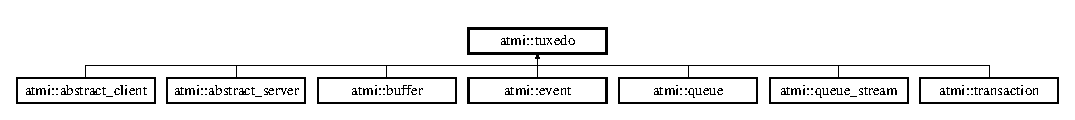
\includegraphics[height=1.435897cm]{classatmi_1_1tuxedo}
\end{center}
\end{figure}
\subsection*{Public Member Functions}
\begin{DoxyCompactItemize}
\item 
char $\ast$ \hyperlink{classatmi_1_1tuxedo_a44e77e3e6216a8c3fb8be33d5d8fed93}{allocate} (const char $\ast$type, const char $\ast$subtype, long size)
\item 
char $\ast$ \hyperlink{classatmi_1_1tuxedo_a683b79440474b94c471ed78ff3775eb8}{extend} (char $\ast$\hyperlink{classatmi_1_1buffer}{buffer}, long extent)
\item 
void \hyperlink{classatmi_1_1tuxedo_afdcf4b7d25862c6fdaeb47d095609a01}{free} (char $\ast$\hyperlink{classatmi_1_1buffer}{buffer})
\item 
int \hyperlink{classatmi_1_1tuxedo_ac702cf5e571a3302978bfa76cd314c9b}{begin} (int timeout=0)
\item 
int \hyperlink{classatmi_1_1tuxedo_aeff1d0270d6b12de07a4478839ec8b07}{commit} ()
\item 
int \hyperlink{classatmi_1_1tuxedo_ac5dbf9db596b4bfa05d0067b8a38e11c}{abort} ()
\item 
long \hyperlink{classatmi_1_1tuxedo_a2f5b4f52ca8095d704dcb23771425690}{error} () const 
\item 
const char $\ast$ \hyperlink{classatmi_1_1tuxedo_ad134373ac62fd2c7e1ac5482bdb7f65e}{error\+\_\+message} () const 
\item 
int \hyperlink{classatmi_1_1tuxedo_a77e2902dcd0293a2127a5d106e566a3b}{errnodetail} () const 
\item 
const char $\ast$ \hyperlink{classatmi_1_1tuxedo_ad7bf2370e3edeb091512d0b640093e9d}{error\+\_\+detail} () const 
\item 
void \hyperlink{classatmi_1_1tuxedo_afa3734356109e8c3ce4d23bfcb94242b}{set\+\_\+context} (T\+P\+C\+O\+N\+T\+E\+X\+T\+\_\+\+T \hyperlink{classatmi_1_1tuxedo_a6d31779e76609264295e0065fdfc008d}{context})
\item 
T\+P\+C\+O\+N\+T\+E\+X\+T\+\_\+\+T \hyperlink{classatmi_1_1tuxedo_a6d31779e76609264295e0065fdfc008d}{context} () const 
\item 
long \hyperlink{classatmi_1_1tuxedo_adfebbea0b6599ba8ca87743c55157b82}{flags} () const 
\item 
void \hyperlink{classatmi_1_1tuxedo_a31eb2881e3b9706c515da03728ab6875}{set\+\_\+flags} (long \hyperlink{classatmi_1_1tuxedo_adfebbea0b6599ba8ca87743c55157b82}{flags})
\item 
void \hyperlink{classatmi_1_1tuxedo_a649b28c90b5f73439e5d2ceb83a43dbd}{reset\+\_\+flags} (long \hyperlink{classatmi_1_1tuxedo_adfebbea0b6599ba8ca87743c55157b82}{flags})
\item 
void \hyperlink{classatmi_1_1tuxedo_aeef30e346c61643db72b255872729633}{unset\+\_\+flags} (long \hyperlink{classatmi_1_1tuxedo_adfebbea0b6599ba8ca87743c55157b82}{flags})
\end{DoxyCompactItemize}
\subsection*{Static Public Attributes}
\begin{DoxyCompactItemize}
\item 
\hypertarget{classatmi_1_1tuxedo_a79d8805a077e30138729f44c75fcfa5d}{static const long \hyperlink{classatmi_1_1tuxedo_a79d8805a077e30138729f44c75fcfa5d}{F\+A\+I\+L\+E\+D} = -\/1}\label{classatmi_1_1tuxedo_a79d8805a077e30138729f44c75fcfa5d}

\begin{DoxyCompactList}\small\item\em Tuxedo error value. \end{DoxyCompactList}\end{DoxyCompactItemize}
\subsection*{Protected Member Functions}
\begin{DoxyCompactItemize}
\item 
void \hyperlink{classatmi_1_1tuxedo_a90d83b2141d484744a82202f3f66a939}{switch\+\_\+context} ()
\item 
void \hyperlink{classatmi_1_1tuxedo_a1c1d7f2df43e4357788d03977548ac2e}{update\+Errno} ()
\item 
{\footnotesize template$<$typename... Args$>$ }\\int \hyperlink{classatmi_1_1tuxedo_ae8715aedf9c8f3178aec71e93ee35be4}{handle\+\_\+tperrno} (int \+\_\+tperrno, const char $\ast$msg, const Args \&...args)
\end{DoxyCompactItemize}
\subsection*{Static Protected Member Functions}
\begin{DoxyCompactItemize}
\item 
static long \hyperlink{classatmi_1_1tuxedo_af962caf2ded45e192ba6a37740b133d0}{unset} (long bits, long \hyperlink{classatmi_1_1tuxedo_adfebbea0b6599ba8ca87743c55157b82}{flags})
\item 
static long \hyperlink{classatmi_1_1tuxedo_a73c4c95f165a052ba5a3a29cb2834831}{set} (long, long)
\end{DoxyCompactItemize}
\subsection*{Protected Attributes}
\begin{DoxyCompactItemize}
\item 
\hypertarget{classatmi_1_1tuxedo_ac0714439c1f2e889190471966c9fda2f}{long \hyperlink{classatmi_1_1tuxedo_ac0714439c1f2e889190471966c9fda2f}{\+\_\+flags}}\label{classatmi_1_1tuxedo_ac0714439c1f2e889190471966c9fda2f}

\begin{DoxyCompactList}\small\item\em Tuxedo flags. \end{DoxyCompactList}\item 
\hypertarget{classatmi_1_1tuxedo_a1193fe16ac0984776678a23da351d00a}{nl\+\_\+catd \hyperlink{classatmi_1_1tuxedo_a1193fe16ac0984776678a23da351d00a}{\+\_\+catd}}\label{classatmi_1_1tuxedo_a1193fe16ac0984776678a23da351d00a}

\begin{DoxyCompactList}\small\item\em message catalog refenence \end{DoxyCompactList}\end{DoxyCompactItemize}


\subsection{Detailed Description}
All common used A\+T\+M\+I method are group in this class.

\begin{DoxyAuthor}{Author}
Herbert Koelman 
\end{DoxyAuthor}


\subsection{Member Function Documentation}
\hypertarget{classatmi_1_1tuxedo_ac5dbf9db596b4bfa05d0067b8a38e11c}{\index{atmi\+::tuxedo@{atmi\+::tuxedo}!abort@{abort}}
\index{abort@{abort}!atmi\+::tuxedo@{atmi\+::tuxedo}}
\subsubsection[{abort}]{\setlength{\rightskip}{0pt plus 5cm}int atmi\+::tuxedo\+::abort (
\begin{DoxyParamCaption}
{}
\end{DoxyParamCaption}
)}}\label{classatmi_1_1tuxedo_ac5dbf9db596b4bfa05d0067b8a38e11c}
Abort X\+A transaction.


\begin{DoxyExceptions}{Exceptions}
{\em transaction\+\_\+exception} & if abort failed. \\
\hline
\end{DoxyExceptions}
\hypertarget{classatmi_1_1tuxedo_a44e77e3e6216a8c3fb8be33d5d8fed93}{\index{atmi\+::tuxedo@{atmi\+::tuxedo}!allocate@{allocate}}
\index{allocate@{allocate}!atmi\+::tuxedo@{atmi\+::tuxedo}}
\subsubsection[{allocate}]{\setlength{\rightskip}{0pt plus 5cm}char $\ast$ atmi\+::tuxedo\+::allocate (
\begin{DoxyParamCaption}
\item[{const char $\ast$}]{type, }
\item[{const char $\ast$}]{subtype, }
\item[{long}]{size}
\end{DoxyParamCaption}
)}}\label{classatmi_1_1tuxedo_a44e77e3e6216a8c3fb8be33d5d8fed93}
Allocate a new buffer.

buffer types provided by tuxedo C\+A\+R\+R\+A\+Y Character array (possibly containing N\+U\+L\+L characters) that is neither encoded nor decoded during transmission S\+T\+R\+I\+N\+G N\+U\+L\+L-\/terminated character array F\+M\+L F\+M\+L fielded buffer V\+I\+E\+W C structure or F\+M\+L view X\+\_\+\+O\+C\+T\+E\+T Equivalent to C\+A\+R\+R\+A\+Y; provided for X\+A\+T\+M\+I compatibility X\+\_\+\+C\+\_\+\+T\+Y\+P\+E Equivalent to V\+I\+E\+W; provided for X\+A\+T\+M\+I compatibility X\+\_\+ C\+O\+M\+M\+O\+N Equivalent to V\+I\+E\+W; provided for X\+A\+T\+M\+I compatibility F\+M\+L32 F\+M\+L32 fielded buffer, using 32-\/bit identifiers and offsets V\+I\+E\+W32 C structure or F\+M\+L32 view, using 32-\/bit identifiers, counter variables, and size variables X\+M\+L buffer for X\+M\+L documents M\+B\+S\+T\+R\+I\+N\+G Character array for multibyte characters

Note that only the first eight bytes of type and the first 16 bytes of subtype are significant.


\begin{DoxyParams}{Parameters}
{\em type} & buffer type to allocate (S\+T\+R\+I\+N\+G, V\+I\+E\+W, F\+M\+L, ...) \\
\hline
{\em subtype} & buffer subtype. N\+U\+L\+L means none \\
\hline
{\em size} & memory size to allocate.\\
\hline
\end{DoxyParams}
\begin{DoxyReturn}{Returns}
allocated buffer or N\+U\+L\+L if failed
\end{DoxyReturn}

\begin{DoxyExceptions}{Exceptions}
{\em \hyperlink{classatmi_1_1tuxedo__exception}{tuxedo\+\_\+exception}} & if something goes wrong. \\
\hline
\end{DoxyExceptions}
\hypertarget{classatmi_1_1tuxedo_ac702cf5e571a3302978bfa76cd314c9b}{\index{atmi\+::tuxedo@{atmi\+::tuxedo}!begin@{begin}}
\index{begin@{begin}!atmi\+::tuxedo@{atmi\+::tuxedo}}
\subsubsection[{begin}]{\setlength{\rightskip}{0pt plus 5cm}int atmi\+::tuxedo\+::begin (
\begin{DoxyParamCaption}
\item[{int}]{timeout = {\ttfamily 0}}
\end{DoxyParamCaption}
)}}\label{classatmi_1_1tuxedo_ac702cf5e571a3302978bfa76cd314c9b}
Starts X\+A transaction.


\begin{DoxyParams}{Parameters}
{\em timeout} & max duration in seconds for a transaction to complete.\\
\hline
\end{DoxyParams}

\begin{DoxyExceptions}{Exceptions}
{\em transaction\+\_\+exception} & is raised upon failure. \\
\hline
\end{DoxyExceptions}
\hypertarget{classatmi_1_1tuxedo_aeff1d0270d6b12de07a4478839ec8b07}{\index{atmi\+::tuxedo@{atmi\+::tuxedo}!commit@{commit}}
\index{commit@{commit}!atmi\+::tuxedo@{atmi\+::tuxedo}}
\subsubsection[{commit}]{\setlength{\rightskip}{0pt plus 5cm}int atmi\+::tuxedo\+::commit (
\begin{DoxyParamCaption}
{}
\end{DoxyParamCaption}
)}}\label{classatmi_1_1tuxedo_aeff1d0270d6b12de07a4478839ec8b07}
Commit X\+A transaction.


\begin{DoxyExceptions}{Exceptions}
{\em transaction\+\_\+exception} & on failure. \\
\hline
\end{DoxyExceptions}
\hypertarget{classatmi_1_1tuxedo_a6d31779e76609264295e0065fdfc008d}{\index{atmi\+::tuxedo@{atmi\+::tuxedo}!context@{context}}
\index{context@{context}!atmi\+::tuxedo@{atmi\+::tuxedo}}
\subsubsection[{context}]{\setlength{\rightskip}{0pt plus 5cm}T\+P\+C\+O\+N\+T\+E\+X\+T\+\_\+\+T atmi\+::tuxedo\+::context (
\begin{DoxyParamCaption}
{}
\end{DoxyParamCaption}
) const\hspace{0.3cm}{\ttfamily [inline]}}}\label{classatmi_1_1tuxedo_a6d31779e76609264295e0065fdfc008d}
\begin{DoxyReturn}{Returns}
the current context 
\end{DoxyReturn}
\hypertarget{classatmi_1_1tuxedo_a77e2902dcd0293a2127a5d106e566a3b}{\index{atmi\+::tuxedo@{atmi\+::tuxedo}!errnodetail@{errnodetail}}
\index{errnodetail@{errnodetail}!atmi\+::tuxedo@{atmi\+::tuxedo}}
\subsubsection[{errnodetail}]{\setlength{\rightskip}{0pt plus 5cm}int atmi\+::tuxedo\+::errnodetail (
\begin{DoxyParamCaption}
{}
\end{DoxyParamCaption}
) const\hspace{0.3cm}{\ttfamily [inline]}}}\label{classatmi_1_1tuxedo_a77e2902dcd0293a2127a5d106e566a3b}
\begin{DoxyReturn}{Returns}
the current error detail (if one exist). 
\end{DoxyReturn}
\hypertarget{classatmi_1_1tuxedo_a2f5b4f52ca8095d704dcb23771425690}{\index{atmi\+::tuxedo@{atmi\+::tuxedo}!error@{error}}
\index{error@{error}!atmi\+::tuxedo@{atmi\+::tuxedo}}
\subsubsection[{error}]{\setlength{\rightskip}{0pt plus 5cm}long atmi\+::tuxedo\+::error (
\begin{DoxyParamCaption}
{}
\end{DoxyParamCaption}
) const\hspace{0.3cm}{\ttfamily [inline]}}}\label{classatmi_1_1tuxedo_a2f5b4f52ca8095d704dcb23771425690}
\begin{DoxyReturn}{Returns}
the current errno value 
\end{DoxyReturn}
\hypertarget{classatmi_1_1tuxedo_ad7bf2370e3edeb091512d0b640093e9d}{\index{atmi\+::tuxedo@{atmi\+::tuxedo}!error\+\_\+detail@{error\+\_\+detail}}
\index{error\+\_\+detail@{error\+\_\+detail}!atmi\+::tuxedo@{atmi\+::tuxedo}}
\subsubsection[{error\+\_\+detail}]{\setlength{\rightskip}{0pt plus 5cm}const char$\ast$ atmi\+::tuxedo\+::error\+\_\+detail (
\begin{DoxyParamCaption}
{}
\end{DoxyParamCaption}
) const\hspace{0.3cm}{\ttfamily [inline]}}}\label{classatmi_1_1tuxedo_ad7bf2370e3edeb091512d0b640093e9d}
\begin{DoxyReturn}{Returns}
an error detail description string (if one exists). 
\end{DoxyReturn}
\hypertarget{classatmi_1_1tuxedo_ad134373ac62fd2c7e1ac5482bdb7f65e}{\index{atmi\+::tuxedo@{atmi\+::tuxedo}!error\+\_\+message@{error\+\_\+message}}
\index{error\+\_\+message@{error\+\_\+message}!atmi\+::tuxedo@{atmi\+::tuxedo}}
\subsubsection[{error\+\_\+message}]{\setlength{\rightskip}{0pt plus 5cm}const char$\ast$ atmi\+::tuxedo\+::error\+\_\+message (
\begin{DoxyParamCaption}
{}
\end{DoxyParamCaption}
) const\hspace{0.3cm}{\ttfamily [inline]}}}\label{classatmi_1_1tuxedo_ad134373ac62fd2c7e1ac5482bdb7f65e}
\begin{DoxyReturn}{Returns}
an error description string of the last errno 
\end{DoxyReturn}
\hypertarget{classatmi_1_1tuxedo_a683b79440474b94c471ed78ff3775eb8}{\index{atmi\+::tuxedo@{atmi\+::tuxedo}!extend@{extend}}
\index{extend@{extend}!atmi\+::tuxedo@{atmi\+::tuxedo}}
\subsubsection[{extend}]{\setlength{\rightskip}{0pt plus 5cm}char $\ast$ atmi\+::tuxedo\+::extend (
\begin{DoxyParamCaption}
\item[{char $\ast$}]{buffer, }
\item[{long}]{extent}
\end{DoxyParamCaption}
)}}\label{classatmi_1_1tuxedo_a683b79440474b94c471ed78ff3775eb8}
resize buffer.


\begin{DoxyParams}{Parameters}
{\em buffer} & buffer to resize (the return value maybe different buffer) \\
\hline
{\em extent} & number of bytes to add \\
\hline
\end{DoxyParams}
\begin{DoxyReturn}{Returns}
reference to resized buffer 
\end{DoxyReturn}
\hypertarget{classatmi_1_1tuxedo_adfebbea0b6599ba8ca87743c55157b82}{\index{atmi\+::tuxedo@{atmi\+::tuxedo}!flags@{flags}}
\index{flags@{flags}!atmi\+::tuxedo@{atmi\+::tuxedo}}
\subsubsection[{flags}]{\setlength{\rightskip}{0pt plus 5cm}long atmi\+::tuxedo\+::flags (
\begin{DoxyParamCaption}
{}
\end{DoxyParamCaption}
) const\hspace{0.3cm}{\ttfamily [inline]}}}\label{classatmi_1_1tuxedo_adfebbea0b6599ba8ca87743c55157b82}
\begin{DoxyReturn}{Returns}
tuxedo flags used by this instance. 
\end{DoxyReturn}
\hypertarget{classatmi_1_1tuxedo_afdcf4b7d25862c6fdaeb47d095609a01}{\index{atmi\+::tuxedo@{atmi\+::tuxedo}!free@{free}}
\index{free@{free}!atmi\+::tuxedo@{atmi\+::tuxedo}}
\subsubsection[{free}]{\setlength{\rightskip}{0pt plus 5cm}void atmi\+::tuxedo\+::free (
\begin{DoxyParamCaption}
\item[{char $\ast$}]{buffer}
\end{DoxyParamCaption}
)}}\label{classatmi_1_1tuxedo_afdcf4b7d25862c6fdaeb47d095609a01}
Free a previously allocated tuxedo buffer. \hypertarget{classatmi_1_1tuxedo_ae8715aedf9c8f3178aec71e93ee35be4}{\index{atmi\+::tuxedo@{atmi\+::tuxedo}!handle\+\_\+tperrno@{handle\+\_\+tperrno}}
\index{handle\+\_\+tperrno@{handle\+\_\+tperrno}!atmi\+::tuxedo@{atmi\+::tuxedo}}
\subsubsection[{handle\+\_\+tperrno}]{\setlength{\rightskip}{0pt plus 5cm}template$<$typename... Args$>$ int atmi\+::tuxedo\+::handle\+\_\+tperrno (
\begin{DoxyParamCaption}
\item[{int}]{\+\_\+tperrno, }
\item[{const char $\ast$}]{msg, }
\item[{const Args \&...}]{args}
\end{DoxyParamCaption}
)\hspace{0.3cm}{\ttfamily [inline]}, {\ttfamily [protected]}}}\label{classatmi_1_1tuxedo_ae8715aedf9c8f3178aec71e93ee35be4}
Triggers exceptions according to the given tperrno passed. The exception will be initialized with msg.


\begin{DoxyParams}{Parameters}
{\em \+\_\+tperrno} & tperrno to handle \\
\hline
{\em msg} & message to setup in thrown exception. \\
\hline
{\em args} & message argument (see printf) \\
\hline
\end{DoxyParams}
\begin{DoxyReturn}{Returns}
legacy will be removed when prototype will be changed to void handle\+\_\+transaction\+\_\+errno() 
\end{DoxyReturn}
\hypertarget{classatmi_1_1tuxedo_a649b28c90b5f73439e5d2ceb83a43dbd}{\index{atmi\+::tuxedo@{atmi\+::tuxedo}!reset\+\_\+flags@{reset\+\_\+flags}}
\index{reset\+\_\+flags@{reset\+\_\+flags}!atmi\+::tuxedo@{atmi\+::tuxedo}}
\subsubsection[{reset\+\_\+flags}]{\setlength{\rightskip}{0pt plus 5cm}void atmi\+::tuxedo\+::reset\+\_\+flags (
\begin{DoxyParamCaption}
\item[{long}]{flags}
\end{DoxyParamCaption}
)\hspace{0.3cm}{\ttfamily [inline]}}}\label{classatmi_1_1tuxedo_a649b28c90b5f73439e5d2ceb83a43dbd}
Reset flag value to T\+P\+N\+O\+F\+L\+A\+G\+S \hypertarget{classatmi_1_1tuxedo_a73c4c95f165a052ba5a3a29cb2834831}{\index{atmi\+::tuxedo@{atmi\+::tuxedo}!set@{set}}
\index{set@{set}!atmi\+::tuxedo@{atmi\+::tuxedo}}
\subsubsection[{set}]{\setlength{\rightskip}{0pt plus 5cm}long atmi\+::tuxedo\+::set (
\begin{DoxyParamCaption}
\item[{long}]{f, }
\item[{long}]{sf}
\end{DoxyParamCaption}
)\hspace{0.3cm}{\ttfamily [static]}, {\ttfamily [protected]}}}\label{classatmi_1_1tuxedo_a73c4c95f165a052ba5a3a29cb2834831}
set bits in second argument in first argument \hypertarget{classatmi_1_1tuxedo_afa3734356109e8c3ce4d23bfcb94242b}{\index{atmi\+::tuxedo@{atmi\+::tuxedo}!set\+\_\+context@{set\+\_\+context}}
\index{set\+\_\+context@{set\+\_\+context}!atmi\+::tuxedo@{atmi\+::tuxedo}}
\subsubsection[{set\+\_\+context}]{\setlength{\rightskip}{0pt plus 5cm}void atmi\+::tuxedo\+::set\+\_\+context (
\begin{DoxyParamCaption}
\item[{T\+P\+C\+O\+N\+T\+E\+X\+T\+\_\+\+T}]{context}
\end{DoxyParamCaption}
)\hspace{0.3cm}{\ttfamily [inline]}}}\label{classatmi_1_1tuxedo_afa3734356109e8c3ce4d23bfcb94242b}
set the tuxedo context to use when calling tuxedo functions(tpsetctxt()).

When set, A\+T\+M\+I++ switches to this context before executing a tuxedo call.


\begin{DoxyParams}{Parameters}
{\em context} & context to be used by this instance \\
\hline
\end{DoxyParams}
\hypertarget{classatmi_1_1tuxedo_a31eb2881e3b9706c515da03728ab6875}{\index{atmi\+::tuxedo@{atmi\+::tuxedo}!set\+\_\+flags@{set\+\_\+flags}}
\index{set\+\_\+flags@{set\+\_\+flags}!atmi\+::tuxedo@{atmi\+::tuxedo}}
\subsubsection[{set\+\_\+flags}]{\setlength{\rightskip}{0pt plus 5cm}void atmi\+::tuxedo\+::set\+\_\+flags (
\begin{DoxyParamCaption}
\item[{long}]{flags}
\end{DoxyParamCaption}
)\hspace{0.3cm}{\ttfamily [inline]}}}\label{classatmi_1_1tuxedo_a31eb2881e3b9706c515da03728ab6875}
Set tuxedo flags \hypertarget{classatmi_1_1tuxedo_a90d83b2141d484744a82202f3f66a939}{\index{atmi\+::tuxedo@{atmi\+::tuxedo}!switch\+\_\+context@{switch\+\_\+context}}
\index{switch\+\_\+context@{switch\+\_\+context}!atmi\+::tuxedo@{atmi\+::tuxedo}}
\subsubsection[{switch\+\_\+context}]{\setlength{\rightskip}{0pt plus 5cm}void atmi\+::tuxedo\+::switch\+\_\+context (
\begin{DoxyParamCaption}
{}
\end{DoxyParamCaption}
)\hspace{0.3cm}{\ttfamily [protected]}}}\label{classatmi_1_1tuxedo_a90d83b2141d484744a82202f3f66a939}
If context is set (context != 0 ), then tpsetctxt is called. This method does nothing otherwise. \hypertarget{classatmi_1_1tuxedo_af962caf2ded45e192ba6a37740b133d0}{\index{atmi\+::tuxedo@{atmi\+::tuxedo}!unset@{unset}}
\index{unset@{unset}!atmi\+::tuxedo@{atmi\+::tuxedo}}
\subsubsection[{unset}]{\setlength{\rightskip}{0pt plus 5cm}long atmi\+::tuxedo\+::unset (
\begin{DoxyParamCaption}
\item[{long}]{bits, }
\item[{long}]{flags}
\end{DoxyParamCaption}
)\hspace{0.3cm}{\ttfamily [static]}, {\ttfamily [protected]}}}\label{classatmi_1_1tuxedo_af962caf2ded45e192ba6a37740b133d0}
Unset bits in second argument from first argument


\begin{DoxyParams}{Parameters}
{\em bits} & bits that should be unset \\
\hline
{\em flags} & flags to unset \\
\hline
\end{DoxyParams}
\hypertarget{classatmi_1_1tuxedo_aeef30e346c61643db72b255872729633}{\index{atmi\+::tuxedo@{atmi\+::tuxedo}!unset\+\_\+flags@{unset\+\_\+flags}}
\index{unset\+\_\+flags@{unset\+\_\+flags}!atmi\+::tuxedo@{atmi\+::tuxedo}}
\subsubsection[{unset\+\_\+flags}]{\setlength{\rightskip}{0pt plus 5cm}void atmi\+::tuxedo\+::unset\+\_\+flags (
\begin{DoxyParamCaption}
\item[{long}]{flags}
\end{DoxyParamCaption}
)\hspace{0.3cm}{\ttfamily [inline]}}}\label{classatmi_1_1tuxedo_aeef30e346c61643db72b255872729633}
unset flags 
\begin{DoxyParams}{Parameters}
{\em flags} & flags to unset \\
\hline
\end{DoxyParams}
\hypertarget{classatmi_1_1tuxedo_a1c1d7f2df43e4357788d03977548ac2e}{\index{atmi\+::tuxedo@{atmi\+::tuxedo}!update\+Errno@{update\+Errno}}
\index{update\+Errno@{update\+Errno}!atmi\+::tuxedo@{atmi\+::tuxedo}}
\subsubsection[{update\+Errno}]{\setlength{\rightskip}{0pt plus 5cm}void atmi\+::tuxedo\+::update\+Errno (
\begin{DoxyParamCaption}
{}
\end{DoxyParamCaption}
)\hspace{0.3cm}{\ttfamily [protected]}}}\label{classatmi_1_1tuxedo_a1c1d7f2df43e4357788d03977548ac2e}
update current errno and sets what must be set.

\begin{DoxyRefDesc}{Deprecated}
\item[\hyperlink{deprecated__deprecated000005}{Deprecated}]we use exception instead \end{DoxyRefDesc}


The documentation for this class was generated from the following files\+:\begin{DoxyCompactItemize}
\item 
include/atmi/tuxedo.\+hpp\item 
src/tuxedo.\+cpp\end{DoxyCompactItemize}

\hypertarget{classatmi_1_1tuxedo__exception}{}\section{atmi\+:\+:tuxedo\+\_\+exception Class Reference}
\label{classatmi_1_1tuxedo__exception}\index{atmi\+::tuxedo\+\_\+exception@{atmi\+::tuxedo\+\_\+exception}}


{\ttfamily \#include $<$exceptions.\+hpp$>$}

Inheritance diagram for atmi\+:\+:tuxedo\+\_\+exception\+:\begin{figure}[H]
\begin{center}
\leavevmode
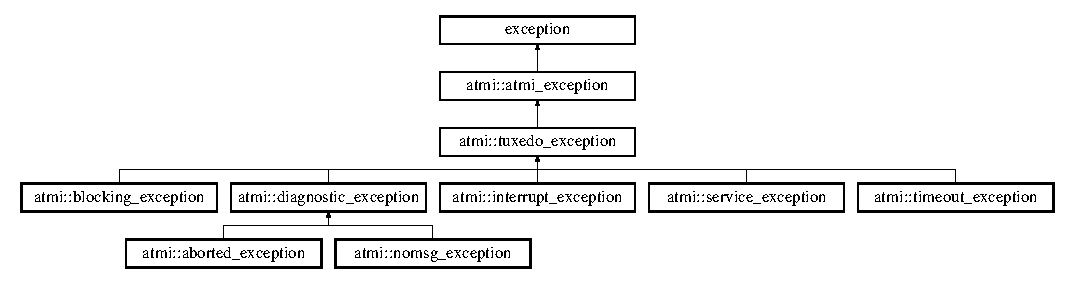
\includegraphics[height=3.373494cm]{classatmi_1_1tuxedo__exception}
\end{center}
\end{figure}
\subsection*{Public Member Functions}
\begin{DoxyCompactItemize}
\item 
{\footnotesize template$<$typename... Args$>$ }\\\hyperlink{classatmi_1_1tuxedo__exception_a6219496e27ade0d5fa67fce17ecea526}{tuxedo\+\_\+exception} (int err, const char $\ast$msg, const Args \&...args)
\item 
virtual int \hyperlink{classatmi_1_1tuxedo__exception_a9299a99da028fde85d8c4d52165a6b1d}{error} () const 
\item 
int \hyperlink{classatmi_1_1tuxedo__exception_ab0dff17c0b6e5af2ba4e9c73029fc41b}{detail} () const 
\item 
virtual const char $\ast$ \hyperlink{classatmi_1_1tuxedo__exception_adcf355cbe82b96ba273fabf6753e3bc7}{error\+\_\+message} () const 
\item 
const char $\ast$ \hyperlink{classatmi_1_1tuxedo__exception_abeb62f07cfb36d1d9d58b6a3aa9ef939}{error\+\_\+detail} () const 
\end{DoxyCompactItemize}
\subsection*{Additional Inherited Members}


\subsection{Detailed Description}
Tuxedo T\+P related exceptions 

\subsection{Constructor \& Destructor Documentation}
\hypertarget{classatmi_1_1tuxedo__exception_a6219496e27ade0d5fa67fce17ecea526}{}\index{atmi\+::tuxedo\+\_\+exception@{atmi\+::tuxedo\+\_\+exception}!tuxedo\+\_\+exception@{tuxedo\+\_\+exception}}
\index{tuxedo\+\_\+exception@{tuxedo\+\_\+exception}!atmi\+::tuxedo\+\_\+exception@{atmi\+::tuxedo\+\_\+exception}}
\subsubsection[{tuxedo\+\_\+exception(int err, const char $\ast$msg, const Args \&...\+args)}]{\setlength{\rightskip}{0pt plus 5cm}template$<$typename... Args$>$ atmi\+::tuxedo\+\_\+exception\+::tuxedo\+\_\+exception (
\begin{DoxyParamCaption}
\item[{int}]{err, }
\item[{const char $\ast$}]{msg, }
\item[{const Args \&...}]{args}
\end{DoxyParamCaption}
)\hspace{0.3cm}{\ttfamily [inline]}}\label{classatmi_1_1tuxedo__exception_a6219496e27ade0d5fa67fce17ecea526}
Tuxedo exceptions.


\begin{DoxyParams}{Parameters}
{\em err} & Ferror32 value \\
\hline
{\em msg} & error message \\
\hline
{\em args} & error message parameters (variadic). \\
\hline
\end{DoxyParams}


\subsection{Member Function Documentation}
\hypertarget{classatmi_1_1tuxedo__exception_ab0dff17c0b6e5af2ba4e9c73029fc41b}{}\index{atmi\+::tuxedo\+\_\+exception@{atmi\+::tuxedo\+\_\+exception}!detail@{detail}}
\index{detail@{detail}!atmi\+::tuxedo\+\_\+exception@{atmi\+::tuxedo\+\_\+exception}}
\subsubsection[{detail() const }]{\setlength{\rightskip}{0pt plus 5cm}int atmi\+::tuxedo\+\_\+exception\+::detail (
\begin{DoxyParamCaption}
{}
\end{DoxyParamCaption}
) const\hspace{0.3cm}{\ttfamily [inline]}}\label{classatmi_1_1tuxedo__exception_ab0dff17c0b6e5af2ba4e9c73029fc41b}
\begin{DoxyReturn}{Returns}
detail error number 
\end{DoxyReturn}
\hypertarget{classatmi_1_1tuxedo__exception_a9299a99da028fde85d8c4d52165a6b1d}{}\index{atmi\+::tuxedo\+\_\+exception@{atmi\+::tuxedo\+\_\+exception}!error@{error}}
\index{error@{error}!atmi\+::tuxedo\+\_\+exception@{atmi\+::tuxedo\+\_\+exception}}
\subsubsection[{error() const }]{\setlength{\rightskip}{0pt plus 5cm}virtual int atmi\+::tuxedo\+\_\+exception\+::error (
\begin{DoxyParamCaption}
{}
\end{DoxyParamCaption}
) const\hspace{0.3cm}{\ttfamily [inline]}, {\ttfamily [virtual]}}\label{classatmi_1_1tuxedo__exception_a9299a99da028fde85d8c4d52165a6b1d}
\begin{DoxyReturn}{Returns}
tperr that raise the exception 
\end{DoxyReturn}
\hypertarget{classatmi_1_1tuxedo__exception_abeb62f07cfb36d1d9d58b6a3aa9ef939}{}\index{atmi\+::tuxedo\+\_\+exception@{atmi\+::tuxedo\+\_\+exception}!error\+\_\+detail@{error\+\_\+detail}}
\index{error\+\_\+detail@{error\+\_\+detail}!atmi\+::tuxedo\+\_\+exception@{atmi\+::tuxedo\+\_\+exception}}
\subsubsection[{error\+\_\+detail() const }]{\setlength{\rightskip}{0pt plus 5cm}const char $\ast$ atmi\+::tuxedo\+\_\+exception\+::error\+\_\+detail (
\begin{DoxyParamCaption}
{}
\end{DoxyParamCaption}
) const}\label{classatmi_1_1tuxedo__exception_abeb62f07cfb36d1d9d58b6a3aa9ef939}
\begin{DoxyReturn}{Returns}
tuxedo error detail string 
\end{DoxyReturn}
\hypertarget{classatmi_1_1tuxedo__exception_adcf355cbe82b96ba273fabf6753e3bc7}{}\index{atmi\+::tuxedo\+\_\+exception@{atmi\+::tuxedo\+\_\+exception}!error\+\_\+message@{error\+\_\+message}}
\index{error\+\_\+message@{error\+\_\+message}!atmi\+::tuxedo\+\_\+exception@{atmi\+::tuxedo\+\_\+exception}}
\subsubsection[{error\+\_\+message() const }]{\setlength{\rightskip}{0pt plus 5cm}const char $\ast$ atmi\+::tuxedo\+\_\+exception\+::error\+\_\+message (
\begin{DoxyParamCaption}
{}
\end{DoxyParamCaption}
) const\hspace{0.3cm}{\ttfamily [virtual]}}\label{classatmi_1_1tuxedo__exception_adcf355cbe82b96ba273fabf6753e3bc7}
\begin{DoxyReturn}{Returns}
tuxedo error message string 
\end{DoxyReturn}


The documentation for this class was generated from the following files\+:\begin{DoxyCompactItemize}
\item 
include/atmi/exceptions.\+hpp\item 
src/exceptions.\+cpp\end{DoxyCompactItemize}

\hypertarget{classatmi_1_1ulog}{\section{atmi\+:\+:ulog Class Reference}
\label{classatmi_1_1ulog}\index{atmi\+::ulog@{atmi\+::ulog}}
}


{\ttfamily \#include $<$ulog.\+hpp$>$}

\subsection*{Public Member Functions}
\begin{DoxyCompactItemize}
\item 
\hyperlink{classatmi_1_1ulog_a52394015e2bcd098c9b6de0e173637e9}{ulog} (\hyperlink{group__logging_gaf9bdc466e66896621125b81d022264ca}{log\+\_\+level} \hyperlink{classatmi_1_1ulog_a75c3bf9fdf68677f5e2b096acdac737e}{level}=log\+\_\+level\+::info)
\item 
{\footnotesize template$<$typename... Args$>$ }\\void \hyperlink{classatmi_1_1ulog_a29e7f8215085533c0b4fb788545e9329}{error} (const std\+::string \&fmt, const Args \&...args)
\item 
{\footnotesize template$<$typename... Args$>$ }\\void \hyperlink{classatmi_1_1ulog_a48f44bc3d0265fdb3b8d464b78894ccc}{warning} (const std\+::string \&fmt, const Args \&...args)
\item 
{\footnotesize template$<$typename... Args$>$ }\\void \hyperlink{classatmi_1_1ulog_a21019f39119ed09e7d71672441456787}{info} (const std\+::string \&fmt, const Args \&...args)
\item 
{\footnotesize template$<$typename... Args$>$ }\\void \hyperlink{classatmi_1_1ulog_a23b79b2222930f4363d3150c39b49992}{finer} (const std\+::string \&fmt, const Args \&...args)
\item 
{\footnotesize template$<$typename... Args$>$ }\\void \hyperlink{classatmi_1_1ulog_a96d76b04d41c2a77a4c88e5d422ea5e5}{debug} (const std\+::string \&fmt, const Args \&...args)
\item 
void \hyperlink{classatmi_1_1ulog_a190ffba6f15d00c21578051ac5c7b035}{set\+\_\+log\+\_\+level} (\hyperlink{group__logging_gaf9bdc466e66896621125b81d022264ca}{log\+\_\+levels} \hyperlink{classatmi_1_1ulog_a75c3bf9fdf68677f5e2b096acdac737e}{level})
\item 
int \hyperlink{classatmi_1_1ulog_a75c3bf9fdf68677f5e2b096acdac737e}{level} () const 
\item 
{\footnotesize template$<$typename... Args$>$ }\\void \hyperlink{classatmi_1_1ulog_ad352992adc121dbdaf0428fd6f53125a}{log} (\hyperlink{group__logging_gaf9bdc466e66896621125b81d022264ca}{log\+\_\+levels} at, const std\+::string \&fmt, const Args \&...args)
\end{DoxyCompactItemize}


\subsection{Detailed Description}
Interface og the logging facility

Verbose is the D\+E\+B\+U\+G log level (level value 0) and least verbose is E\+R\+R\+O\+R (level value 4). Write messages that matches the current level value and above. 

\subsection{Constructor \& Destructor Documentation}
\hypertarget{classatmi_1_1ulog_a52394015e2bcd098c9b6de0e173637e9}{\index{atmi\+::ulog@{atmi\+::ulog}!ulog@{ulog}}
\index{ulog@{ulog}!atmi\+::ulog@{atmi\+::ulog}}
\subsubsection[{ulog}]{\setlength{\rightskip}{0pt plus 5cm}atmi\+::ulog\+::ulog (
\begin{DoxyParamCaption}
\item[{{\bf log\+\_\+level}}]{level = {\ttfamily log\+\_\+level\+:\+:info}}
\end{DoxyParamCaption}
)\hspace{0.3cm}{\ttfamily [explicit]}}}\label{classatmi_1_1ulog_a52394015e2bcd098c9b6de0e173637e9}
create a U\+L\+O\+G instance.

Default is log\+\_\+atmi\+::levels\+::info


\begin{DoxyParams}{Parameters}
{\em level} & wanted log level \\
\hline
\end{DoxyParams}


\subsection{Member Function Documentation}
\hypertarget{classatmi_1_1ulog_a96d76b04d41c2a77a4c88e5d422ea5e5}{\index{atmi\+::ulog@{atmi\+::ulog}!debug@{debug}}
\index{debug@{debug}!atmi\+::ulog@{atmi\+::ulog}}
\subsubsection[{debug}]{\setlength{\rightskip}{0pt plus 5cm}template$<$typename... Args$>$ void atmi\+::ulog\+::debug (
\begin{DoxyParamCaption}
\item[{const std\+::string \&}]{fmt, }
\item[{const Args \&...}]{args}
\end{DoxyParamCaption}
)\hspace{0.3cm}{\ttfamily [inline]}}}\label{classatmi_1_1ulog_a96d76b04d41c2a77a4c88e5d422ea5e5}
debug message


\begin{DoxyParams}{Parameters}
{\em fmt} & message format( see stdd\+:pritnf()) \\
\hline
{\em args} & format arguments \\
\hline
\end{DoxyParams}
\hypertarget{classatmi_1_1ulog_a29e7f8215085533c0b4fb788545e9329}{\index{atmi\+::ulog@{atmi\+::ulog}!error@{error}}
\index{error@{error}!atmi\+::ulog@{atmi\+::ulog}}
\subsubsection[{error}]{\setlength{\rightskip}{0pt plus 5cm}template$<$typename... Args$>$ void atmi\+::ulog\+::error (
\begin{DoxyParamCaption}
\item[{const std\+::string \&}]{fmt, }
\item[{const Args \&...}]{args}
\end{DoxyParamCaption}
)\hspace{0.3cm}{\ttfamily [inline]}}}\label{classatmi_1_1ulog_a29e7f8215085533c0b4fb788545e9329}
error message


\begin{DoxyParams}{Parameters}
{\em fmt} & message format( see stdd\+:pritnf()) \\
\hline
{\em args} & format arguments \\
\hline
\end{DoxyParams}
\hypertarget{classatmi_1_1ulog_a23b79b2222930f4363d3150c39b49992}{\index{atmi\+::ulog@{atmi\+::ulog}!finer@{finer}}
\index{finer@{finer}!atmi\+::ulog@{atmi\+::ulog}}
\subsubsection[{finer}]{\setlength{\rightskip}{0pt plus 5cm}template$<$typename... Args$>$ void atmi\+::ulog\+::finer (
\begin{DoxyParamCaption}
\item[{const std\+::string \&}]{fmt, }
\item[{const Args \&...}]{args}
\end{DoxyParamCaption}
)\hspace{0.3cm}{\ttfamily [inline]}}}\label{classatmi_1_1ulog_a23b79b2222930f4363d3150c39b49992}
finer message


\begin{DoxyParams}{Parameters}
{\em fmt} & message format( see stdd\+:pritnf()) \\
\hline
{\em args} & format arguments \\
\hline
\end{DoxyParams}
\hypertarget{classatmi_1_1ulog_a21019f39119ed09e7d71672441456787}{\index{atmi\+::ulog@{atmi\+::ulog}!info@{info}}
\index{info@{info}!atmi\+::ulog@{atmi\+::ulog}}
\subsubsection[{info}]{\setlength{\rightskip}{0pt plus 5cm}template$<$typename... Args$>$ void atmi\+::ulog\+::info (
\begin{DoxyParamCaption}
\item[{const std\+::string \&}]{fmt, }
\item[{const Args \&...}]{args}
\end{DoxyParamCaption}
)\hspace{0.3cm}{\ttfamily [inline]}}}\label{classatmi_1_1ulog_a21019f39119ed09e7d71672441456787}
info message


\begin{DoxyParams}{Parameters}
{\em fmt} & message format( see stdd\+:pritnf()) \\
\hline
{\em args} & format arguments \\
\hline
\end{DoxyParams}
\hypertarget{classatmi_1_1ulog_a75c3bf9fdf68677f5e2b096acdac737e}{\index{atmi\+::ulog@{atmi\+::ulog}!level@{level}}
\index{level@{level}!atmi\+::ulog@{atmi\+::ulog}}
\subsubsection[{level}]{\setlength{\rightskip}{0pt plus 5cm}int atmi\+::ulog\+::level (
\begin{DoxyParamCaption}
{}
\end{DoxyParamCaption}
) const\hspace{0.3cm}{\ttfamily [inline]}}}\label{classatmi_1_1ulog_a75c3bf9fdf68677f5e2b096acdac737e}
\begin{DoxyReturn}{Returns}
current log level 
\end{DoxyReturn}
\hypertarget{classatmi_1_1ulog_ad352992adc121dbdaf0428fd6f53125a}{\index{atmi\+::ulog@{atmi\+::ulog}!log@{log}}
\index{log@{log}!atmi\+::ulog@{atmi\+::ulog}}
\subsubsection[{log}]{\setlength{\rightskip}{0pt plus 5cm}template$<$typename... Args$>$ void atmi\+::ulog\+::log (
\begin{DoxyParamCaption}
\item[{{\bf log\+\_\+levels}}]{at, }
\item[{const std\+::string \&}]{fmt, }
\item[{const Args \&...}]{args}
\end{DoxyParamCaption}
)\hspace{0.3cm}{\ttfamily [inline]}}}\label{classatmi_1_1ulog_ad352992adc121dbdaf0428fd6f53125a}
Actual log writer


\begin{DoxyParams}{Parameters}
{\em at} & the level to which this message correspond's \\
\hline
{\em fmt} & message to log \\
\hline
{\em args} & substitution arguments of the message. \\
\hline
\end{DoxyParams}
\hypertarget{classatmi_1_1ulog_a190ffba6f15d00c21578051ac5c7b035}{\index{atmi\+::ulog@{atmi\+::ulog}!set\+\_\+log\+\_\+level@{set\+\_\+log\+\_\+level}}
\index{set\+\_\+log\+\_\+level@{set\+\_\+log\+\_\+level}!atmi\+::ulog@{atmi\+::ulog}}
\subsubsection[{set\+\_\+log\+\_\+level}]{\setlength{\rightskip}{0pt plus 5cm}void atmi\+::ulog\+::set\+\_\+log\+\_\+level (
\begin{DoxyParamCaption}
\item[{{\bf log\+\_\+levels}}]{level}
\end{DoxyParamCaption}
)}}\label{classatmi_1_1ulog_a190ffba6f15d00c21578051ac5c7b035}
Set a new logging level 
\begin{DoxyParams}{Parameters}
{\em level} & level from which the ulog starts to write messages \\
\hline
\end{DoxyParams}
\hypertarget{classatmi_1_1ulog_a48f44bc3d0265fdb3b8d464b78894ccc}{\index{atmi\+::ulog@{atmi\+::ulog}!warning@{warning}}
\index{warning@{warning}!atmi\+::ulog@{atmi\+::ulog}}
\subsubsection[{warning}]{\setlength{\rightskip}{0pt plus 5cm}template$<$typename... Args$>$ void atmi\+::ulog\+::warning (
\begin{DoxyParamCaption}
\item[{const std\+::string \&}]{fmt, }
\item[{const Args \&...}]{args}
\end{DoxyParamCaption}
)\hspace{0.3cm}{\ttfamily [inline]}}}\label{classatmi_1_1ulog_a48f44bc3d0265fdb3b8d464b78894ccc}
warning message


\begin{DoxyParams}{Parameters}
{\em fmt} & message format( see stdd\+:pritnf()) \\
\hline
{\em args} & format arguments \\
\hline
\end{DoxyParams}


The documentation for this class was generated from the following files\+:\begin{DoxyCompactItemize}
\item 
include/atmi/ulog.\+hpp\item 
src/ulog.\+cpp\end{DoxyCompactItemize}

\hypertarget{classatmi_1_1unix__exception}{}\section{atmi\+:\+:unix\+\_\+exception Class Reference}
\label{classatmi_1_1unix__exception}\index{atmi\+::unix\+\_\+exception@{atmi\+::unix\+\_\+exception}}


{\ttfamily \#include $<$exceptions.\+hpp$>$}

Inheritance diagram for atmi\+:\+:unix\+\_\+exception\+:\begin{figure}[H]
\begin{center}
\leavevmode
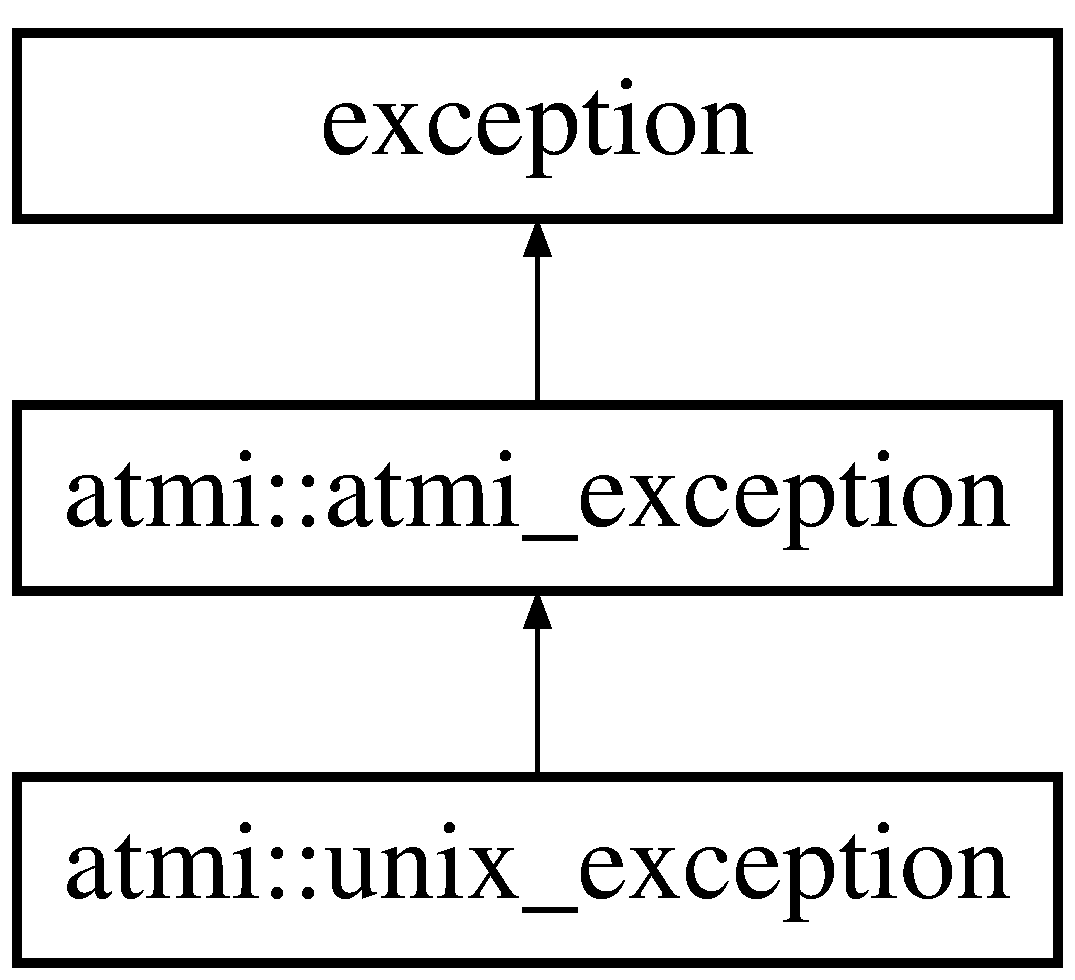
\includegraphics[height=3.000000cm]{classatmi_1_1unix__exception}
\end{center}
\end{figure}
\subsection*{Public Member Functions}
\begin{DoxyCompactItemize}
\item 
{\footnotesize template$<$typename... Args$>$ }\\\hyperlink{classatmi_1_1unix__exception_a0e296d42c4d9e4008e0f3b920fe453ae}{unix\+\_\+exception} (int err, const char $\ast$msg, const Args \&...args)
\item 
{\footnotesize template$<$typename... Args$>$ }\\\hyperlink{classatmi_1_1unix__exception_aec5e09afab40d70b2b4d9aa314a5b71b}{unix\+\_\+exception} (const char $\ast$msg, const Args \&...args)
\item 
\hyperlink{classatmi_1_1unix__exception_aeba0ddfd609e50f3bdf03b7208fdcc3d}{unix\+\_\+exception} ()
\item 
int \hyperlink{classatmi_1_1unix__exception_a4aab55cca505c04ea9e1c65b8cc0c254}{error} () const 
\end{DoxyCompactItemize}
\subsection*{Additional Inherited Members}


\subsection{Detailed Description}
Unix related exceptions.

This exception can be used to return a system error. 

\subsection{Constructor \& Destructor Documentation}
\index{atmi\+::unix\+\_\+exception@{atmi\+::unix\+\_\+exception}!unix\+\_\+exception@{unix\+\_\+exception}}
\index{unix\+\_\+exception@{unix\+\_\+exception}!atmi\+::unix\+\_\+exception@{atmi\+::unix\+\_\+exception}}
\subsubsection[{\texorpdfstring{unix\+\_\+exception(int err, const char $\ast$msg, const Args \&...\+args)}{unix\_exception(int err, const char *msg, const Args \&...args)}}]{\setlength{\rightskip}{0pt plus 5cm}template$<$typename... Args$>$ atmi\+::unix\+\_\+exception\+::unix\+\_\+exception (
\begin{DoxyParamCaption}
\item[{int}]{err, }
\item[{const char $\ast$}]{msg, }
\item[{const Args \&...}]{args}
\end{DoxyParamCaption}
)\hspace{0.3cm}{\ttfamily [inline]}}\hypertarget{classatmi_1_1unix__exception_a0e296d42c4d9e4008e0f3b920fe453ae}{}\label{classatmi_1_1unix__exception_a0e296d42c4d9e4008e0f3b920fe453ae}
new unix exception.


\begin{DoxyParams}{Parameters}
{\em err} & errno value \\
\hline
{\em msg} & error message \\
\hline
{\em args} & error message parameters (variadic). \\
\hline
\end{DoxyParams}
\index{atmi\+::unix\+\_\+exception@{atmi\+::unix\+\_\+exception}!unix\+\_\+exception@{unix\+\_\+exception}}
\index{unix\+\_\+exception@{unix\+\_\+exception}!atmi\+::unix\+\_\+exception@{atmi\+::unix\+\_\+exception}}
\subsubsection[{\texorpdfstring{unix\+\_\+exception(const char $\ast$msg, const Args \&...\+args)}{unix\_exception(const char *msg, const Args \&...args)}}]{\setlength{\rightskip}{0pt plus 5cm}template$<$typename... Args$>$ atmi\+::unix\+\_\+exception\+::unix\+\_\+exception (
\begin{DoxyParamCaption}
\item[{const char $\ast$}]{msg, }
\item[{const Args \&...}]{args}
\end{DoxyParamCaption}
)\hspace{0.3cm}{\ttfamily [inline]}}\hypertarget{classatmi_1_1unix__exception_aec5e09afab40d70b2b4d9aa314a5b71b}{}\label{classatmi_1_1unix__exception_aec5e09afab40d70b2b4d9aa314a5b71b}
new unix exception.

error is defaulted to errno


\begin{DoxyParams}{Parameters}
{\em msg} & error message \\
\hline
{\em args} & error message parameters (variadic). \\
\hline
\end{DoxyParams}
\index{atmi\+::unix\+\_\+exception@{atmi\+::unix\+\_\+exception}!unix\+\_\+exception@{unix\+\_\+exception}}
\index{unix\+\_\+exception@{unix\+\_\+exception}!atmi\+::unix\+\_\+exception@{atmi\+::unix\+\_\+exception}}
\subsubsection[{\texorpdfstring{unix\+\_\+exception()}{unix\_exception()}}]{\setlength{\rightskip}{0pt plus 5cm}atmi\+::unix\+\_\+exception\+::unix\+\_\+exception (
\begin{DoxyParamCaption}
{}
\end{DoxyParamCaption}
)}\hypertarget{classatmi_1_1unix__exception_aeba0ddfd609e50f3bdf03b7208fdcc3d}{}\label{classatmi_1_1unix__exception_aeba0ddfd609e50f3bdf03b7208fdcc3d}
default constructor.

set error message to strerror. 

\subsection{Member Function Documentation}
\index{atmi\+::unix\+\_\+exception@{atmi\+::unix\+\_\+exception}!error@{error}}
\index{error@{error}!atmi\+::unix\+\_\+exception@{atmi\+::unix\+\_\+exception}}
\subsubsection[{\texorpdfstring{error() const }{error() const }}]{\setlength{\rightskip}{0pt plus 5cm}int atmi\+::unix\+\_\+exception\+::error (
\begin{DoxyParamCaption}
{}
\end{DoxyParamCaption}
) const}\hypertarget{classatmi_1_1unix__exception_a4aab55cca505c04ea9e1c65b8cc0c254}{}\label{classatmi_1_1unix__exception_a4aab55cca505c04ea9e1c65b8cc0c254}
\begin{DoxyReturn}{Returns}
unix errno 
\end{DoxyReturn}


The documentation for this class was generated from the following files\+:\begin{DoxyCompactItemize}
\item 
include/atmi/exceptions.\+hpp\item 
src/exceptions.\+cpp\end{DoxyCompactItemize}

\chapter{Example Documentation}
\hypertarget{buffer_test_8bcl-example}{\section{buffer\+\_\+test.\+bcl}
}
A fielded buffers, that contain attribute-\/value pairs called fields.

The attribute is the field’s identifier, and the associated value represents the field’s data content. Fielded buffers provide an excellent structure for communicating parameterized data between cooperating processes, by providing named access to a set of related fields. Programs that need to communicate with other processes can use the F\+M\+L software to provide access to fields without concerning themselves with the structures containing them.

\begin{DoxyAuthor}{Author}
herbert koelman(\href{mailto:herbert.koelman@me.com}{\tt herbert.\+koelman@me.\+com})
\end{DoxyAuthor}

\begin{DoxyCodeInclude}
1 /* $Id$
2 
3    Sample Tuxedo client using ATMI++ libray.
4 
5  */
6 #include <stdlib.h>
7 #include <unistd.h>
8 #include <string.h>
9 #include <string>
10 #include <iostream>
11 #include <fstream>
12 #include <typeinfo>
13 #include "atmi/atmi++.hpp"
14 
15 #include "sample\_fml\_table.h"
16 
17 class buffer\_test : public atmi::abstract\_client \{
18   public:
19     buffer\_test (): atmi::abstract\_client ("btest")\{
20     \};
21 
22     int run ( int argc, char **argv )\{
23       try \{
24 
25         atmi::buffer b (100), a;
26         /*
27            const char *types[5] = \{ typeid(short).name(), typeid(int).name() \};
28            std::cout << "Stored: " << types[0] << std::endl;
29            std::cout << "Stored: " << types[1] << " is a " << std::endl;
30            if(strcmp ( typeid(int).name(), types[1]) == 0 )\{
31            std::cout << "same type int." << std::endl;
32            \}
33            std::cout << "Type id " << typeid(long).name() << std::endl;
34          */
35 
36         std::cout << "atmi::buffer b: " << b.used() << "/" << b.unused() <<", size: " << b.size() << ",
       chksum: " << b.chksum() <<  std::endl;
37 
38         atmi::Tfield<atmi::carray>   unknown\_field;
39         unknown\_field.set\_id(SRVCDAY);
40         unknown\_field.set\_char\_array("salut les amis\(\backslash\)0rray", sizeof ("salut les amis\(\backslash\)0rray"));
41 
42         atmi::Tfield<string> prenom ( EMPNAME );
43         atmi::Tfield<long>   empid ( EMPID );
44         atmi::Tfield<long>   empzip ( EMPZIP );
45         atmi::Tfield<string> nom ( EMPNAME );
46         atmi::Tfield<char *> carray ( SRVCDAY );
47         atmi::Tfield<char *> copy ( SRVCDAY );
48 
49         prenom = "herbert";
50         nom = "this is a char *";
51         empid = 2;
52         carray.set\_char\_array("helloworld\(\backslash\)0rray", strlen ("helloworld\(\backslash\)0rray"));
53         copy = carray;
54 
55         std::cout << "Added fields: " << std::endl;
56         b.add(unknown\_field);
57         b.add ( empid );
58         b.add ( nom );
59         b.add ( prenom );
60         b.add ( carray );
61         b.print ();
62 
63         b.get ( copy );
64 
65         std::cout << copy.what() << std::endl;
66         long len = 5;                  //copy.length();
67         char *cav = new char[len];
68         copy.get\_char\_array ( cav, len );
69         for ( int x = 0; x < len; x++ ) \{
70           std::cout << "'"<< cav[x]<<"',";
71         \}
72         std::cout << std::endl;
73 
74         std::cout << "Setting (update) empid value: " << std::endl;
75         empid = 22;
76         b.set ( empid );
77         b.print ();
78 
79         std::cout << "size : " << b.size();
80         b.pack ();
81         std::cout << ", after pack: " << b.size() << std::endl;
82 
83         std::cout << "atmi::buffer (in the end): " << b.used() << "/" << b.unused() <<", size: " <<
       b.size() << ", chksum: " << b.chksum() <<  std::endl;
84 
85         std::cout << "wrapping atmi::buffer." << std::endl ;
86         atmi::buffer wrapper ( b.get\_buffer());
87         nom = "this was added into a wrapper instance of atmi::buffer.";
88         wrapper.set (nom );
89         wrapper.print ();
90 
91         std::cout << "transforming a atmi::buffer into a wrapped buffer." << std::endl;
92         atmi::buffer wrapper1;
93         wrapper1.set\_buffer ( wrapper.get\_buffer());
94         prenom = "this was set by a wrapper";
95         wrapper1.set ( prenom );
96         wrapper1.print();
97 
98       \}catch ( atmi::buffer\_exception &err ) \{
99         cerr << err.what() << ". Ferror : " << err.error() <<std::endl;
100       \} catch ( atmi::atmi\_exception &err ) \{
101         cerr << err.what() << std::endl;
102       \} catch ( std::exception &err ) \{
103         cerr << err.what() << std::endl;
104       \}
105 
106       return 9999;
107     \}
108 
109 \};
110 
111 // program main -------------------------------------------------
112 
113 int main ( int argc, char **argv ) \{
114 
115   try \{
116 
117     std::cout << "atmi::buffer sample program (" << atmi::cpp\_atmi\_version() <<")." << std::endl;
118     std::cout << "setting up";
119     buffer\_test btest;
120 
121     std::cout << ", starting up" ;
122     btest.run ( argc, argv );
123 
124   \} catch ( atmi::atmi\_exception &err)\{
125     cerr << std::endl << err.what() << std::endl;
126   \} catch ( std::exception &err ) \{
127     cerr << std::endl << err.what() << std::endl;
128   \}
129   std::cout << ", done." << std::endl;
130 
131   return 0;
132 \}
\end{DoxyCodeInclude}
 
\hypertarget{qexport_8bcl-example}{\section{qexport.\+bcl}
}
Global utility to stream out the content of a queue


\begin{DoxyParams}{Parameters}
{\em out} & output stream \\
\hline
{\em qs} & queue stream that will handle the reading of messages\\
\hline
\end{DoxyParams}

\begin{DoxyCodeInclude}
1 #include "options.hpp"
2 #include <atmi/atmi++.hpp>
3 #include <cstdlib>
4 #include <ostream>
5 #include <fstream>
6 #include <csignal>
7 
8 bool running = true ;
9 
10 void signal\_handler( int signal )\{ //NOSONAR what the heck is this warning !?
11     running=false;
12 \}
13 
14 /** export messages found in a given queue
15  *
16  */
17 class queue\_export: public atmi::abstract\_client \{
18   public:
19 
20     queue\_export(const char *pname, const char *user, const char *sys\_passwd, const char *app\_passwd, const
       char *group, int wait = 0 ):
21       abstract\_client(pname, user, sys\_passwd, app\_passwd, group)\{
22     \}
23 
24     int run (const char *qspace, const char *queue, size\_t buffer\_size, std::ostream &out, bool daemon) \{
25 
26       auto status = EXIT\_FAILURE;
27 
28       try \{
29 
30 #       ifdef DEBUG
31         printf("DEBUG %s: exporting messages found in queue [%s] from queue space [%s], daemon mode %s,
       buffer size: %d bytes\(\backslash\)n", \_\_FUNCTION\_\_,
32             queue,
33             qspace,
34             daemon ? "true" : "false",
35             buffer\_size);
36 #       endif
37 
38         atmi::queue\_ptr q = new\_queue\_instance(qspace, queue);
39         q->set\_message\_wait(false); // don't wait for messages
40 
41         long counter = 0;
42 
43         atmi::queue\_stream qs(*q, buffer\_size);
44         do \{
45           out << qs ; // write messages
46           out.flush();
47 
48           counter += qs.count();
49 
50 #       ifdef DEBUG
51         printf("DEBUG %s (line %d): flushed stream, running %s, daemon %s\(\backslash\)n", \_\_FUNCTION\_\_, \_\_LINE\_\_,
52           running ? "true" : "false",
53           daemon  ? "true" : "false"
54           );
55 #       endif
56         \}while( running && daemon);
57 
58         std::cerr << "exported " << counter << " messages from " << queue << "." << std::endl ;
59 
60         status = EXIT\_SUCCESS ;
61 
62       \} catch ( std::exception &err )\{
63         std::cerr << err.what() << std::endl ;
64       \}
65 
66 #     ifdef DEBUG
67       std::cout << "type enter to exit." << std::endl;
68       std::string buffer;
69       std::getline (std::cin,buffer);
70 #     endif
71 
72       return status ;
73     \}
74 \};
75 
76 int main ( int argc, char *argv[] )\{
77 
78   auto status = EXIT\_FAILURE ;
79   try \{
80 
81     signal(SIGINT, signal\_handler);
82     char *pname = basename(argv[0]);
83 
84     export\_options options;
85     options.parse(argc, argv);
86 
87     if ( (options.qspace != NULL) && (options.queue != NULL) )\{
88       queue\_export qexport(pname, options.user, options.sys\_passwd, options.app\_passwd, options.group);
89       if ( options.output\_file != NULL ) \{
90         std::ifstream file;
91         file.open(options.output\_file,std::ofstream::out | std::ofstream::app);
92         if (file.is\_open())\{
93           std::ostream out(file.rdbuf());
94           status = qexport.run(options.qspace, options.queue, options.buffer\_size, out, options.daemon);
95         \} else \{
96           perror("failed to open export destination file");
97         \}
98       \} else \{
99         std::ostream out(std::cout.rdbuf()); // fall back to stdou
100         status = qexport.run(options.qspace, options.queue, options.buffer\_size, out, options.daemon);
101       \}
102 
103     \}else\{
104       std::cerr << "missing arguments, please provide a queue space and queue name (-q)." << std::endl;
105       options.usage(pname, "send messages found in a queue to stdout or a file (if last argument is
       passed).");
106     \}
107 
108   \}catch ( std::exception &err)\{
109     std::cerr << err.what() << std::endl ;
110   \}
111 
112   return status ;
113 \}
\end{DoxyCodeInclude}
 
\hypertarget{qimport_8bcl-example}{\section{qimport.\+bcl}
}
Global utility to stream messages in a queue


\begin{DoxyParams}{Parameters}
{\em in} & input stream \\
\hline
{\em qs} & queue stream that handles the writing of messages to\\
\hline
\end{DoxyParams}

\begin{DoxyCodeInclude}
1 #include "options.hpp"
2 #include <atmi/atmi++.hpp>
3 #include <cstdlib>
4 #include <ostream>
5 #include <fstream>
6 #include <csignal>
7 
8 /** import messages in a given queue
9  *
10  */
11 class queue\_import: public atmi::abstract\_client \{
12   public:
13 
14     queue\_import(const char *pname, const char *user, const char *passwd, const char *group, int wait = 0
       ): abstract\_client(pname, user, passwd, group)\{
15     \}
16 
17     int run (const char *qspace, const char *queue, size\_t buffer\_size, std::istream &in) \{
18 
19       auto status = EXIT\_FAILURE;
20 
21       try \{
22 
23 #       ifdef DEBUG
24         printf("DEBUG %s (%d): exporting messages mporting in queue [%s] from queue space [%s], buffer
       size: %d bytes\(\backslash\)n", \_\_FUNCTION\_\_,\_\_LINE\_\_,
25             queue,
26             qspace,
27             buffer\_size);
28 #       endif
29 
30         atmi::queue\_ptr q = new\_queue\_instance(qspace, queue);
31 
32         long counter = 0;
33 
34         atmi::queue\_stream qs(*q, buffer\_size);
35         in >> qs ;
36 
37         std::cerr << "imported " << qs.count() << " messages in " << queue << "." << std::endl ;
38 
39         status = EXIT\_SUCCESS ;
40 
41       \} catch ( std::exception &err )\{
42         std::cerr << err.what() << std::endl ;
43       \}
44 
45 #     ifdef DEBUG
46       std::cout << "type enter to exit." << std::endl;
47       std::string buffer;
48       std::getline (std::cin,buffer);
49 #     endif
50 
51       return status ;
52     \}
53 \};
54 
55 int main ( int argc, char *argv[] )\{
56 
57   auto status = EXIT\_FAILURE ;
58   try \{
59     char *pname = basename(argv[0]);
60 
61     import\_options options;
62     options.parse(argc, argv);
63 
64     if ( (options.qspace != NULL) && (options.queue != NULL) )\{
65       queue\_import qimport(pname, options.user, options.passwd, options.group);
66       if ( optind < argc ) \{ // consider firt left argument as a path to a file
67         for( ; optind < argc ; optind++ )\{
68           std::ifstream file;
69           file.open(argv[optind],std::ofstream::in);
70           if (file.is\_open())\{
71             std::istream in(file.rdbuf());
72             status = qimport.run(options.qspace, options.queue, options.buffer\_size, in);
73           \} else \{
74             perror("failed to open import file");
75           \}
76         \}
77       \} else \{
78         std::istream in(std::cin.rdbuf()); // fall back to stdou
79         status = qimport.run(options.qspace, options.queue, options.buffer\_size, in);
80       \}
81 
82     \}else\{
83       std::cerr << "missing arguments, please provide a queue space and queue name (-q)." << std::endl;
84       options.usage(pname, "load messages in a queue.");
85     \}
86 
87   \}catch ( std::exception &err)\{
88     std::cerr << err.what() << std::endl ;
89   \}
90 
91   return status ;
92 \}
\end{DoxyCodeInclude}
 
%--- End generated contents ---

% Index
\newpage
\phantomsection
\addcontentsline{toc}{chapter}{Index}
\printindex

\end{document}
